%----------------------------------------------------------------------------------------
%	PACKAGES AND OTHER DOCUMENT CONFIGURATIONS
%----------------------------------------------------------------------------------------

\documentclass[11pt,fleqn]{book} % Default font size and left-justified equations
\hfuzz=100pt 
\hbadness=100000
\usepackage{silence}
\WarningsOff
% does not work
%\WarningFilter{latex}{Overfull}
%\WarningFilter{latex}{Underfull}
\usepackage{marginnote}
%\usepackage[top=1.5cm, bottom=1.5cm, outer=5cm, inner=2cm, heightrounded, marginparwidth=2.5cm, marginparsep=2cm]{geometry}


\newcommand{\video}[3]{%
{\em \href{#3}{
\includegraphics[width=1cm]{images/video.png} #2 (#1)}}    \index{Video!#2 (#1)}
}

\newcommand{\slides}[3]{%
  {\em \href{#3}{
\includegraphics[width=1cm]{images/slide.png} #1}} \index{Slides!#1 (#2)}
}




%----------------------------------------------------------------------------------------
% remove pandoc commands
%----------------------------------------------------------------------------------------
\newcommand{\tightlist}{}
\newenvironment{Shaded}{}{}
\newenvironment{Highlighting}{}{}
\newcommand{\ConstantTok}[1]{\textcolor[rgb]{0.53,0.00,0.00}{{#1}}}
\newcommand{\SpecialCharTok}[1]{\textcolor[rgb]{0.25,0.44,0.63}{{#1}}}
\newcommand{\VerbatimStringTok}[1]{\textcolor[rgb]{0.25,0.44,0.63}{{#1}}}
\newcommand{\SpecialStringTok}[1]{\textcolor[rgb]{0.73,0.40,0.53}{{#1}}}
\newcommand{\ImportTok}[1]{{#1}}
\newcommand{\DocumentationTok}[1]{\textcolor[rgb]{0.73,0.13,0.13}{\textit{{#1}}}}
\newcommand{\AnnotationTok}[1]{\textcolor[rgb]{0.38,0.63,0.69}{\textbf{\textit{{#1}}}}}
\newcommand{\CommentVarTok}[1]{\textcolor[rgb]{0.38,0.63,0.69}{\textbf{\textit{{#1}}}}}
\newcommand{\VariableTok}[1]{\textcolor[rgb]{0.10,0.09,0.49}{{#1}}}
\newcommand{\ControlFlowTok}[1]{\textcolor[rgb]{0.00,0.44,0.13}{\textbf{{#1}}}}
\newcommand{\OperatorTok}[1]{\textcolor[rgb]{0.40,0.40,0.40}{{#1}}}
\newcommand{\BuiltInTok}[1]{{#1}}
\newcommand{\ExtensionTok}[1]{{#1}}
\newcommand{\PreprocessorTok}[1]{\textcolor[rgb]{0.74,0.48,0.00}{{#1}}}
\newcommand{\AttributeTok}[1]{\textcolor[rgb]{0.49,0.56,0.16}{{#1}}}
\newcommand{\InformationTok}[1]{\textcolor[rgb]{0.38,0.63,0.69}{\textbf{\textit{{#1}}}}}
\newcommand{\WarningTok}[1]{\textcolor[rgb]{0.38,0.63,0.69}{\textbf{\textit{{#1}}}}}
\newcommand{\KeywordTok}[1]{\textcolor[rgb]{0.00,0.44,0.13}{\textbf{{#1}}}}
\newcommand{\DataTypeTok}[1]{\textcolor[rgb]{0.56,0.13,0.00}{{#1}}}
\newcommand{\DecValTok}[1]{\textcolor[rgb]{0.25,0.63,0.44}{{#1}}}
\newcommand{\BaseNTok}[1]{\textcolor[rgb]{0.25,0.63,0.44}{{#1}}}
\newcommand{\FloatTok}[1]{\textcolor[rgb]{0.25,0.63,0.44}{{#1}}}
\newcommand{\CharTok}[1]{\textcolor[rgb]{0.25,0.44,0.63}{{#1}}}
\newcommand{\StringTok}[1]{\textcolor[rgb]{0.25,0.44,0.63}{{#1}}}
\newcommand{\CommentTok}[1]{\textcolor[rgb]{0.38,0.63,0.69}{\textit{{#1}}}}
\newcommand{\OtherTok}[1]{\textcolor[rgb]{0.00,0.44,0.13}{{#1}}}
\newcommand{\AlertTok}[1]{\textcolor[rgb]{1.00,0.00,0.00}{\textbf{{#1}}}}
\newcommand{\FunctionTok}[1]{\textcolor[rgb]{0.02,0.16,0.49}{{#1}}}
\newcommand{\RegionMarkerTok}[1]{{#1}}
\newcommand{\ErrorTok}[1]{\textcolor[rgb]{1.00,0.00,0.00}{\textbf{{#1}}}}
\newcommand{\NormalTok}[1]{{#1}}

%----------------------------------------------------------------------------------------

%%%%%%%%%%%%%%%%%%%%%%%%%%%%%%%%%%%%%%%%%
% Modified from 
% by Gregor von Laszewski
%
% The Legrand Orange Book
% Structural Definitions File
% Version 2.0 (9/2/15)
%
% Original author:
% Mathias Legrand (legrand.mathias@gmail.com) with modifications by:
% Vel (vel@latextemplates.com)
% 
% This file has been downloaded from:
% http://www.LaTeXTemplates.com
%
% License:
% CC BY-NC-SA 3.0 (http://creativecommons.org/licenses/by-nc-sa/3.0/)
%
%%%%%%%%%%%%%%%%%%%%%%%%%%%%%%%%%%%%%%%%%

\hfuzz=100pt 
\hbadness=100000
\usepackage{silence}
\WarningsOff
% does not work
%\WarningFilter{latex}{Overfull}
%\WarningFilter{latex}{Underfull}
%\usepackage{marginnote}
\usepackage{currfile}
%\usepackage[top=1.5cm, bottom=1.5cm, outer=5cm, inner=2cm, heightrounded, marginparwidth=2.5cm, marginparsep=2cm]{geometry}

%----------------------------------------------------------------------------------------
%	VARIOUS REQUIRED PACKAGES AND CONFIGURATIONS
%----------------------------------------------------------------------------------------
\usepackage[top=3cm,bottom=3cm,left=3cm,right=3cm,headsep=10pt,a4paper]{geometry} % Page margins

%\usepackage{tipa}
\usepackage{markdown}
\usepackage{todonotes}
\usepackage{fancyvrb}
\usepackage{parskip}
\usepackage{comment}
\usepackage{longtable}
\parindent 0pt
\setlength{\parskip}{6pt}


\usepackage{graphicx} % Required for including pictures
\graphicspath{{./}{images/}} % Specifies the directory where pictures are stored

\usepackage{lipsum} % Inserts dummy text

\usepackage{tikz} % Required for drawing custom shapes

\usepackage[english]{babel} % English language/hyphenation

\usepackage{enumitem} % Customize lists
\setlist{nolistsep} % Reduce spacing between bullet points and numbered lists

\usepackage{booktabs} % Required for nicer horizontal rules in tables

\usepackage{xcolor} % Required for specifying colors by name
%\definecolor{ocre}{RGB}{243,102,25} % Define the orange color used for
%                                % highlighting throughout the book
\definecolor{ocre}{RGB}{65,105,225} % Define the orange color used for
                                % highlighting throughout the book


\usepackage{nameref}
\usepackage{listings}
\usepackage[most]{tcolorbox}
\usepackage{datetime}
\usepackage{minted}


%----------------------------------------------------------------------------------------
%	FONTS
%----------------------------------------------------------------------------------------

\usepackage{avant} % Use the Avantgarde font for headings
%\usepackage{times} % Use the Times font for headings
\usepackage{mathptmx} % Use the Adobe Times Roman as the default text font together with math symbols from the Sym­bol, Chancery and Com­puter Modern fonts

\usepackage{microtype} % Slightly tweak font spacing for aesthetics
\usepackage[utf8]{inputenc} % Required for including letters with accents
\usepackage[T1]{fontenc} % Use 8-bit encoding that has 256 glyphs

%----------------------------------------------------------------------------------------
%	BIBLIOGRAPHY AND INDEX
%----------------------------------------------------------------------------------------

\usepackage[style=numeric,citestyle=numeric,sorting=nyt,sortcites=true,autopunct=true,%
            babel=hyphen,hyperref=true,abbreviate=false,backref=true,backend=biber]{biblatex}
\addbibresource{bib/bibliography.bib} % BibTeX bibliography file
\addbibresource{bib/refs-jabref.bib} % BibTeX bibliography file
\defbibheading{bibempty}{}

\usepackage{calc} % For simpler calculation - used for spacing the index letter headings correctly
\usepackage{makeidx} % Required to make an index
\makeindex % Tells LaTeX to create the files required for indexing

%----------------------------------------------------------------------------------------
%	MAIN TABLE OF CONTENTS
%----------------------------------------------------------------------------------------

\usepackage{titletoc} % Required for manipulating the table of contents

\contentsmargin{0cm} % Removes the default margin

% Part text styling
\titlecontents{part}[0cm]
{\addvspace{20pt}\centering\large\bfseries}
{}
{}
{}

% Chapter text styling
\titlecontents{chapter}[1.25cm] % Indentation
{\addvspace{12pt}\large\sffamily\bfseries} % Spacing and font options for chapters
{\color{ocre!60}\contentslabel[\Large\thecontentslabel]{1.25cm}\color{ocre}} % Chapter number
{\color{ocre}}  
{\color{ocre!60}\normalsize\;\titlerule*[.5pc]{.}\;\thecontentspage} % Page number

% Section text styling
\titlecontents{section}[1.25cm] % Indentation
{\addvspace{3pt}\sffamily\bfseries} % Spacing and font options for sections
{\contentslabel[\thecontentslabel]{1.25cm}} % Section number
{}
{\hfill\color{black}\thecontentspage} % Page number
[]

% Subsection text styling
\titlecontents{subsection}[1.25cm] % Indentation
{\addvspace{1pt}\sffamily\small} % Spacing and font options for subsections
{\contentslabel[\thecontentslabel]{1.25cm}} % Subsection number
{}
{\ \titlerule*[.5pc]{.}\;\thecontentspage} % Page number
[]

% List of figures
\titlecontents{figure}[0em]
{\addvspace{-5pt}\sffamily}
{\thecontentslabel\hspace*{1em}}
{}
{\ \titlerule*[.5pc]{.}\;\thecontentspage}
[]

% List of tables
\titlecontents{table}[0em]
{\addvspace{-5pt}\sffamily}
{\thecontentslabel\hspace*{1em}}
{}
{\ \titlerule*[.5pc]{.}\;\thecontentspage}
[]

%----------------------------------------------------------------------------------------
%	MINI TABLE OF CONTENTS IN PART HEADS
%----------------------------------------------------------------------------------------

% Chapter text styling
\titlecontents{lchapter}[0em] % Indenting
{\addvspace{15pt}\large\sffamily\bfseries} % Spacing and font options for chapters
{\color{ocre}\contentslabel[\Large\thecontentslabel]{1.25cm}\color{ocre}} % Chapter number
{}  
{\color{ocre}\normalsize\sffamily\bfseries\;\titlerule*[.5pc]{.}\;\thecontentspage} % Page number

% Section text styling
\titlecontents{lsection}[0em] % Indenting
{\sffamily\small} % Spacing and font options for sections
{\contentslabel[\thecontentslabel]{1.25cm}} % Section number
{}
{}

% Subsection text styling
\titlecontents{lsubsection}[.5em] % Indentation
{\normalfont\footnotesize\sffamily} % Font settings
{}
{}
{}

%----------------------------------------------------------------------------------------
%	VERBATIM
%----------------------------------------------------------------------------------------

\usepackage{fancyvrb}

%----------------------------------------------------------------------------------------
%	PAGE HEADERS
%----------------------------------------------------------------------------------------


\usepackage{fancyhdr} % Required for header and footer configuration

\pagestyle{fancy}
\renewcommand{\chaptermark}[1]{\markboth{\sffamily\normalsize\bfseries\chaptername\ \thechapter.\ #1}{}} % Chapter text font settings
\renewcommand{\sectionmark}[1]{\markright{\sffamily\normalsize\thesection\hspace{5pt}#1}{}} % Section text font settings
\fancyhf{} \fancyhead[LE,RO]{\sffamily\normalsize\thepage} % Font setting for the page number in the header
\fancyhead[LO]{\rightmark} % Print the nearest section name on the left side of odd pages
\fancyhead[RE]{\leftmark} % Print the current chapter name on the right side of even pages
\renewcommand{\headrulewidth}{0.5pt} % Width of the rule under the header
\addtolength{\headheight}{2.5pt} % Increase the spacing around the header slightly
\renewcommand{\footrulewidth}{0pt} % Removes the rule in the footer
\fancypagestyle{plain}{\fancyhead{}\renewcommand{\headrulewidth}{0pt}} % Style for when a plain pagestyle is specified

% Removes the header from odd empty pages at the end of chapters
\makeatletter
\renewcommand{\cleardoublepage}{
\clearpage\ifodd\c@page\else
\hbox{}
\vspace*{\fill}
\thispagestyle{empty}
\newpage
\fi}

%----------------------------------------------------------------------------------------
%	THEOREM STYLES
%----------------------------------------------------------------------------------------


\usepackage{amsmath,amsfonts,amssymb,amsthm} % For math equations, theorems, symbols, etc

\newcommand{\intoo}[2]{\mathopen{]}#1\,;#2\mathclose{[}}
\newcommand{\ud}{\mathop{\mathrm{{}d}}\mathopen{}}
\newcommand{\intff}[2]{\mathopen{[}#1\,;#2\mathclose{]}}
\newtheorem{notation}{Notation}[chapter]

% Boxed/framed environments
\newtheoremstyle{ocrenumbox}% % Theorem style name
{0pt}% Space above
{0pt}% Space below
{\normalfont}% % Body font
{}% Indent amount
{\small\bf\sffamily\color{ocre}}% % Theorem head font
{\;}% Punctuation after theorem head
{0.25em}% Space after theorem head
{\small\sffamily\color{ocre}\thmname{#1}\nobreakspace\thmnumber{\@ifnotempty{#1}{}\@upn{#2}}% Theorem text (e.g. Theorem 2.1)
\thmnote{\nobreakspace\the\thm@notefont\sffamily\bfseries\color{black}---\nobreakspace#3.}} % Optional theorem note
\renewcommand{\qedsymbol}{$\blacksquare$}% Optional qed square

\newtheoremstyle{blacknumex}% Theorem style name
{5pt}% Space above
{5pt}% Space below
{\normalfont}% Body font
{} % Indent amount
{\small\bf\sffamily}% Theorem head font
{\;}% Punctuation after theorem head
{0.25em}% Space after theorem head
{\small\sffamily{\tiny\ensuremath{\blacksquare}}\nobreakspace\thmname{#1}\nobreakspace\thmnumber{\@ifnotempty{#1}{}\@upn{#2}}% Theorem text (e.g. Theorem 2.1)
\thmnote{\nobreakspace\the\thm@notefont\sffamily\bfseries---\nobreakspace#3.}}% Optional theorem note

\newtheoremstyle{blacknumbox} % Theorem style name
{0pt}% Space above
{0pt}% Space below
{\normalfont}% Body font
{}% Indent amount
{\small\bf\sffamily}% Theorem head font
{\;}% Punctuation after theorem head
{0.25em}% Space after theorem head
{\small\sffamily\thmname{#1}\nobreakspace\thmnumber{\@ifnotempty{#1}{}\@upn{#2}}% Theorem text (e.g. Theorem 2.1)
\thmnote{\nobreakspace\the\thm@notefont\sffamily\bfseries---\nobreakspace#3.}}% Optional theorem note

% Non-boxed/non-framed environments
\newtheoremstyle{ocrenum}% % Theorem style name
{5pt}% Space above
{5pt}% Space below
{\normalfont}% % Body font
{}% Indent amount
{\small\bf\sffamily\color{ocre}}% % Theorem head font
{\;}% Punctuation after theorem head
{0.25em}% Space after theorem head
{\small\sffamily\color{ocre}\thmname{#1}\nobreakspace\thmnumber{\@ifnotempty{#1}{}\@upn{#2}}% Theorem text (e.g. Theorem 2.1)
\thmnote{\nobreakspace\the\thm@notefont\sffamily\bfseries\color{black}---\nobreakspace#3.}} % Optional theorem note
\renewcommand{\qedsymbol}{$\blacksquare$}% Optional qed square
\makeatother

% Defines the theorem text style for each type of theorem to one of the three styles above
\newcounter{dummy} 
\numberwithin{dummy}{section}
\theoremstyle{ocrenumbox}
\newtheorem{theoremeT}[dummy]{Theorem}
\newtheorem{problem}{Problem}[chapter]
\newtheorem{exerciseT}{Exercise}[chapter]
\theoremstyle{blacknumex}
\newtheorem{exampleT}{Example}[chapter]
\theoremstyle{blacknumbox}
\newtheorem{vocabulary}{Vocabulary}[chapter]
\newtheorem{definitionT}{Definition}[section]
\newtheorem{corollaryT}[dummy]{Corollary}
\theoremstyle{ocrenum}
\newtheorem{proposition}[dummy]{Proposition}

%----------------------------------------------------------------------------------------
%	DEFINITION OF COLORED BOXES
%----------------------------------------------------------------------------------------

\RequirePackage[framemethod=default]{mdframed} % Required for creating the theorem, definition, exercise and corollary boxes

% Theorem box
\newmdenv[skipabove=7pt,
skipbelow=7pt,
backgroundcolor=black!5,
linecolor=ocre,
innerleftmargin=5pt,
innerrightmargin=5pt,
innertopmargin=5pt,
leftmargin=0cm,
rightmargin=0cm,
innerbottommargin=5pt]{tBox}

% Exercise box	  
\newmdenv[skipabove=7pt,
skipbelow=7pt,
rightline=false,
leftline=true,
topline=false,
bottomline=false,
backgroundcolor=ocre!10,
linecolor=ocre,
innerleftmargin=5pt,
innerrightmargin=5pt,
innertopmargin=5pt,
innerbottommargin=5pt,
leftmargin=0cm,
rightmargin=0cm,
linewidth=4pt]{eBox}	

% Definition box
\newmdenv[skipabove=7pt,
skipbelow=7pt,
rightline=false,
leftline=true,
topline=false,
bottomline=false,
linecolor=ocre,
innerleftmargin=5pt,
innerrightmargin=5pt,
innertopmargin=0pt,
leftmargin=0cm,
rightmargin=0cm,
linewidth=4pt,
innerbottommargin=0pt]{dBox}	

% Corollary box
\newmdenv[skipabove=7pt,
skipbelow=7pt,
rightline=false,
leftline=true,
topline=false,
bottomline=false,
linecolor=gray,
backgroundcolor=black!5,
innerleftmargin=5pt,
innerrightmargin=5pt,
innertopmargin=5pt,
leftmargin=0cm,
rightmargin=0cm,
linewidth=4pt,
innerbottommargin=5pt]{cBox}

% Creates an environment for each type of theorem and assigns it a theorem text style from the "Theorem Styles" section above and a colored box from above
\newenvironment{theorem}{\begin{tBox}\begin{theoremeT}}{\end{theoremeT}\end{tBox}}
\newenvironment{exercise}{\begin{eBox}\begin{exerciseT}}{\hfill{\color{ocre}\tiny\ensuremath{\blacksquare}}\end{exerciseT}\end{eBox}}				  
\newenvironment{definition}{\begin{dBox}\begin{definitionT}}{\end{definitionT}\end{dBox}}	
\newenvironment{example}{\begin{exampleT}}{\hfill{\tiny\ensuremath{\blacksquare}}\end{exampleT}}		
\newenvironment{corollary}{\begin{cBox}\begin{corollaryT}}{\end{corollaryT}\end{cBox}}	

%----------------------------------------------------------------------------------------
%	REMARK ENVIRONMENT
%----------------------------------------------------------------------------------------

\newenvironment{remark}{\par\vspace{10pt}\small % Vertical white space above the remark and smaller font size
\begin{list}{}{
\leftmargin=35pt % Indentation on the left
\rightmargin=25pt}\item\ignorespaces % Indentation on the right
\makebox[-2.5pt]{\begin{tikzpicture}[overlay]
\node[draw=ocre!60,line width=1pt,circle,fill=ocre!25,font=\sffamily\bfseries,inner sep=2pt,outer sep=0pt] at (-15pt,0pt){\textcolor{ocre}{R}};\end{tikzpicture}} % Orange R in a circle
\advance\baselineskip -1pt}{\end{list}\vskip5pt} % Tighter line spacing and white space after remark

\newenvironment{fileremark}{\par\vspace{10pt}\small % Vertical white space above the remark and smaller font size
\begin{list}{}{
\leftmargin=35pt % Indentation on the left
\rightmargin=25pt}\item\ignorespaces % Indentation on the right
\makebox[-2.5pt]{\begin{tikzpicture}[overlay]
\node[draw=ocre!60,line width=1pt,circle,fill=ocre!25,font=\sffamily\bfseries,inner sep=2pt,outer sep=0pt] at (-15pt,0pt){\textcolor{ocre}{F}};\end{tikzpicture}} % Orange F in a circle
\advance\baselineskip -1pt}{\end{list}\vskip5pt} % Tighter line spacing and white space after remark

\newenvironment{changeremark}{\par\vspace{10pt}\small % Vertical white space above the remark and smaller font size
\begin{list}{}{
\leftmargin=35pt % Indentation on the left
\rightmargin=25pt}\item\ignorespaces % Indentation on the right
\makebox[-2.5pt]{\begin{tikzpicture}[overlay]
\node[draw=ocre!60,line width=1pt,circle,fill=ocre!25,font=\sffamily\bfseries,inner sep=2pt,outer sep=0pt] at (-15pt,0pt){\textcolor{red}{C}};\end{tikzpicture}} % Orange C in a circle
\advance\baselineskip -1pt}{\end{list}\vskip5pt} % Tighter line spacing and white space after remark

\newenvironment{videomark}{\par\vspace{10pt}\small % Vertical white space above the remark and smaller font size
\begin{list}{}{
\leftmargin=35pt % Indentation on the left
\rightmargin=25pt}\item\ignorespaces % Indentation on the right
\makebox[-2.5pt]{\begin{tikzpicture}[overlay]
\node[draw=ocre!60,line width=1pt,circle,fill=ocre!25,font=\sffamily\bfseries,inner sep=2pt,outer sep=0pt] at (-15pt,0pt){\textcolor{ocre}{V}};\end{tikzpicture}} % Orange V in a circle
\advance\baselineskip -1pt}{\end{list}\vskip5pt} % Tighter line spacing and white space after remark

%----------------------------------------------------------------------------------------
%	SECTION NUMBERING IN THE MARGIN
%----------------------------------------------------------------------------------------

\makeatletter
\renewcommand{\@seccntformat}[1]{\llap{\textcolor{ocre}{\csname the#1\endcsname}\hspace{1em}}}                    
\renewcommand{\section}{\@startsection{section}{1}{\z@}
{-4ex \@plus -1ex \@minus -.4ex}
{1ex \@plus.2ex }
{\normalfont\large\sffamily\bfseries}}
\renewcommand{\subsection}{\@startsection {subsection}{2}{\z@}
{-3ex \@plus -0.1ex \@minus -.4ex}
{0.5ex \@plus.2ex }
{\normalfont\sffamily\bfseries}}
\renewcommand{\subsubsection}{\@startsection {subsubsection}{3}{\z@}
{-2ex \@plus -0.1ex \@minus -.2ex}
{.2ex \@plus.2ex }
{\normalfont\small\sffamily\bfseries}}                        
\renewcommand\paragraph{\@startsection{paragraph}{4}{\z@}
{-2ex \@plus-.2ex \@minus .2ex}
{.1ex}
{\normalfont\small\sffamily\bfseries}}

%----------------------------------------------------------------------------------------
%	PART HEADINGS
%----------------------------------------------------------------------------------------

% numbered part in the table of contents
\newcommand{\@mypartnumtocformat}[2]{%
\setlength\fboxsep{0pt}%
\noindent\colorbox{ocre!20}{\strut\parbox[c][.7cm]{\ecart}{\color{ocre!70}\Large\sffamily\bfseries\centering#1}}\hskip\esp\colorbox{ocre!40}{\strut\parbox[c][.7cm]{\linewidth-\ecart-\esp}{\Large\sffamily\centering#2}}}%
%%%%%%%%%%%%%%%%%%%%%%%%%%%%%%%%%%
% unnumbered part in the table of contents
\newcommand{\@myparttocformat}[1]{%
\setlength\fboxsep{0pt}%
\noindent\colorbox{ocre!40}{\strut\parbox[c][.7cm]{\linewidth}{\Large\sffamily\centering#1}}}%
%%%%%%%%%%%%%%%%%%%%%%%%%%%%%%%%%%
\newlength\esp
\setlength\esp{4pt}
\newlength\ecart
\setlength\ecart{1.2cm-\esp}
\newcommand{\thepartimage}{}%
\newcommand{\partimage}[1]{\renewcommand{\thepartimage}{#1}}%
\def\@part[#1]#2{%
\ifnum \c@secnumdepth >-2\relax%
\refstepcounter{part}%
\addcontentsline{toc}{part}{\texorpdfstring{\protect\@mypartnumtocformat{\thepart}{#1}}{\partname~\thepart\ ---\ #1}}
\else%
\addcontentsline{toc}{part}{\texorpdfstring{\protect\@myparttocformat{#1}}{#1}}%
\fi%
\startcontents%
\markboth{}{}%
{\thispagestyle{empty}%
\begin{tikzpicture}[remember picture,overlay]%
\node at (current page.north west){\begin{tikzpicture}[remember picture,overlay]%	
\fill[ocre!20](0cm,0cm) rectangle (\paperwidth,-\paperheight);
\node[anchor=north] at (4cm,-3.25cm){\color{ocre!40}\fontsize{220}{100}\sffamily\bfseries\thepart}; 
\node[anchor=south east] at (\paperwidth-1cm,-\paperheight+1cm){\parbox[t][][t]{8.5cm}{
\printcontents{l}{0}{\setcounter{tocdepth}{1}}%
}};
\node[anchor=north east] at (\paperwidth-1.5cm,-3.25cm){\parbox[t][][t]{15cm}{\strut\raggedleft\color{white}\fontsize{30}{30}\sffamily\bfseries#2}};
\end{tikzpicture}};
\end{tikzpicture}}%
\@endpart}
\def\@spart#1{%
\startcontents%
\phantomsection
{\thispagestyle{empty}%
\begin{tikzpicture}[remember picture,overlay]%
\node at (current page.north west){\begin{tikzpicture}[remember picture,overlay]%	
\fill[ocre!20](0cm,0cm) rectangle (\paperwidth,-\paperheight);
\node[anchor=north east] at (\paperwidth-1.5cm,-3.25cm){\parbox[t][][t]{15cm}{\strut\raggedleft\color{white}\fontsize{30}{30}\sffamily\bfseries#1}};
\end{tikzpicture}};
\end{tikzpicture}}
\addcontentsline{toc}{part}{\texorpdfstring{%
\setlength\fboxsep{0pt}%
\noindent\protect\colorbox{ocre!40}{\strut\protect\parbox[c][.7cm]{\linewidth}{\Large\sffamily\protect\centering #1\quad\mbox{}}}}{#1}}%
\@endpart}
\def\@endpart{\vfil\newpage
\if@twoside
\if@openright
\null
\thispagestyle{empty}%
\newpage
\fi
\fi
\if@tempswa
\twocolumn
\fi}

%----------------------------------------------------------------------------------------
%	CHAPTER HEADINGS
%----------------------------------------------------------------------------------------

% A switch to conditionally include a picture, implemented by  Christian Hupfer
\newif\ifusechapterimage
\usechapterimagetrue
\newcommand{\thechapterimage}{}%
\newcommand{\chapterimage}[1]{\ifusechapterimage\renewcommand{\thechapterimage}{#1}\fi}%
\newcommand{\autodot}{.}
\def\@makechapterhead#1{%
{\parindent \z@ \raggedright \normalfont
\ifnum \c@secnumdepth >\m@ne
\if@mainmatter
\begin{tikzpicture}[remember picture,overlay]
\node at (current page.north west)
{\begin{tikzpicture}[remember picture,overlay]
\node[anchor=north west,inner sep=0pt] at (0,0) {\ifusechapterimage\includegraphics[width=\paperwidth]{\thechapterimage}\fi};
\draw[anchor=west] (\Gm@lmargin,-9cm) node [line width=2pt,rounded corners=15pt,draw=ocre,fill=white,fill opacity=0.5,inner sep=15pt]{\strut\makebox[22cm]{}};
\draw[anchor=west] (\Gm@lmargin+.3cm,-9cm) node {\huge\sffamily\bfseries\color{black}\thechapter\autodot~#1\strut};
\end{tikzpicture}};
\end{tikzpicture}
\else
\begin{tikzpicture}[remember picture,overlay]
\node at (current page.north west)
{\begin{tikzpicture}[remember picture,overlay]
\node[anchor=north west,inner sep=0pt] at (0,0) {\ifusechapterimage\includegraphics[width=\paperwidth]{\thechapterimage}\fi};
\draw[anchor=west] (\Gm@lmargin,-9cm) node [line width=2pt,rounded corners=15pt,draw=ocre,fill=white,fill opacity=0.5,inner sep=15pt]{\strut\makebox[22cm]{}};
\draw[anchor=west] (\Gm@lmargin+.3cm,-9cm) node {\huge\sffamily\bfseries\color{black}#1\strut};
\end{tikzpicture}};
\end{tikzpicture}
\fi\fi\par\vspace*{270\p@}}}

%-------------------------------------------

\def\@makeschapterhead#1{%
\begin{tikzpicture}[remember picture,overlay]
\node at (current page.north west)
{\begin{tikzpicture}[remember picture,overlay]
\node[anchor=north west,inner sep=0pt] at (0,0) {\ifusechapterimage\includegraphics[width=\paperwidth]{\thechapterimage}\fi};
\draw[anchor=west] (\Gm@lmargin,-9cm) node [line width=2pt,rounded corners=15pt,draw=ocre,fill=white,fill opacity=0.5,inner sep=15pt]{\strut\makebox[22cm]{}};
\draw[anchor=west] (\Gm@lmargin+.3cm,-9cm) node {\huge\sffamily\bfseries\color{black}#1\strut};
\end{tikzpicture}};
\end{tikzpicture}
\par\vspace*{270\p@}}
\makeatother

%----------------------------------------------------------------------------------------
%	HYPERLINKS IN THE DOCUMENTS
%----------------------------------------------------------------------------------------

\usepackage{hyperref}
%\usepackage[colorlinks=true,
%            linkcolor=red,
%            urlcolor=blue,
%            citecolor=blue]{hyperref}
\hypersetup{hidelinks,backref=true,pagebackref=true,hyperindex=true,colorlinks=true,linkcolor=blue,citecolor=blue,breaklinks=true,urlcolor=blue,bookmarks=true,bookmarksopen=false,pdftitle={Title},pdfauthor={Author}}
\usepackage{bookmark}
\bookmarksetup{
open,
numbered,
addtohook={%
\ifnum\bookmarkget{level}=0 % chapter
\bookmarksetup{bold}%
\fi
\ifnum\bookmarkget{level}=-1 % part
\bookmarksetup{color=ocre,bold}%
\fi
}
}
 % Insert the commands.tex file which contains the majority of the structure behind the template

\begin{document}

%----------------------------------------------------------------------------------------
%	TITLE PAGE
%----------------------------------------------------------------------------------------

\begingroup
\thispagestyle{empty}
\begin{tikzpicture}[remember picture,overlay]
\node[inner sep=0pt] (background) at (current page.center) {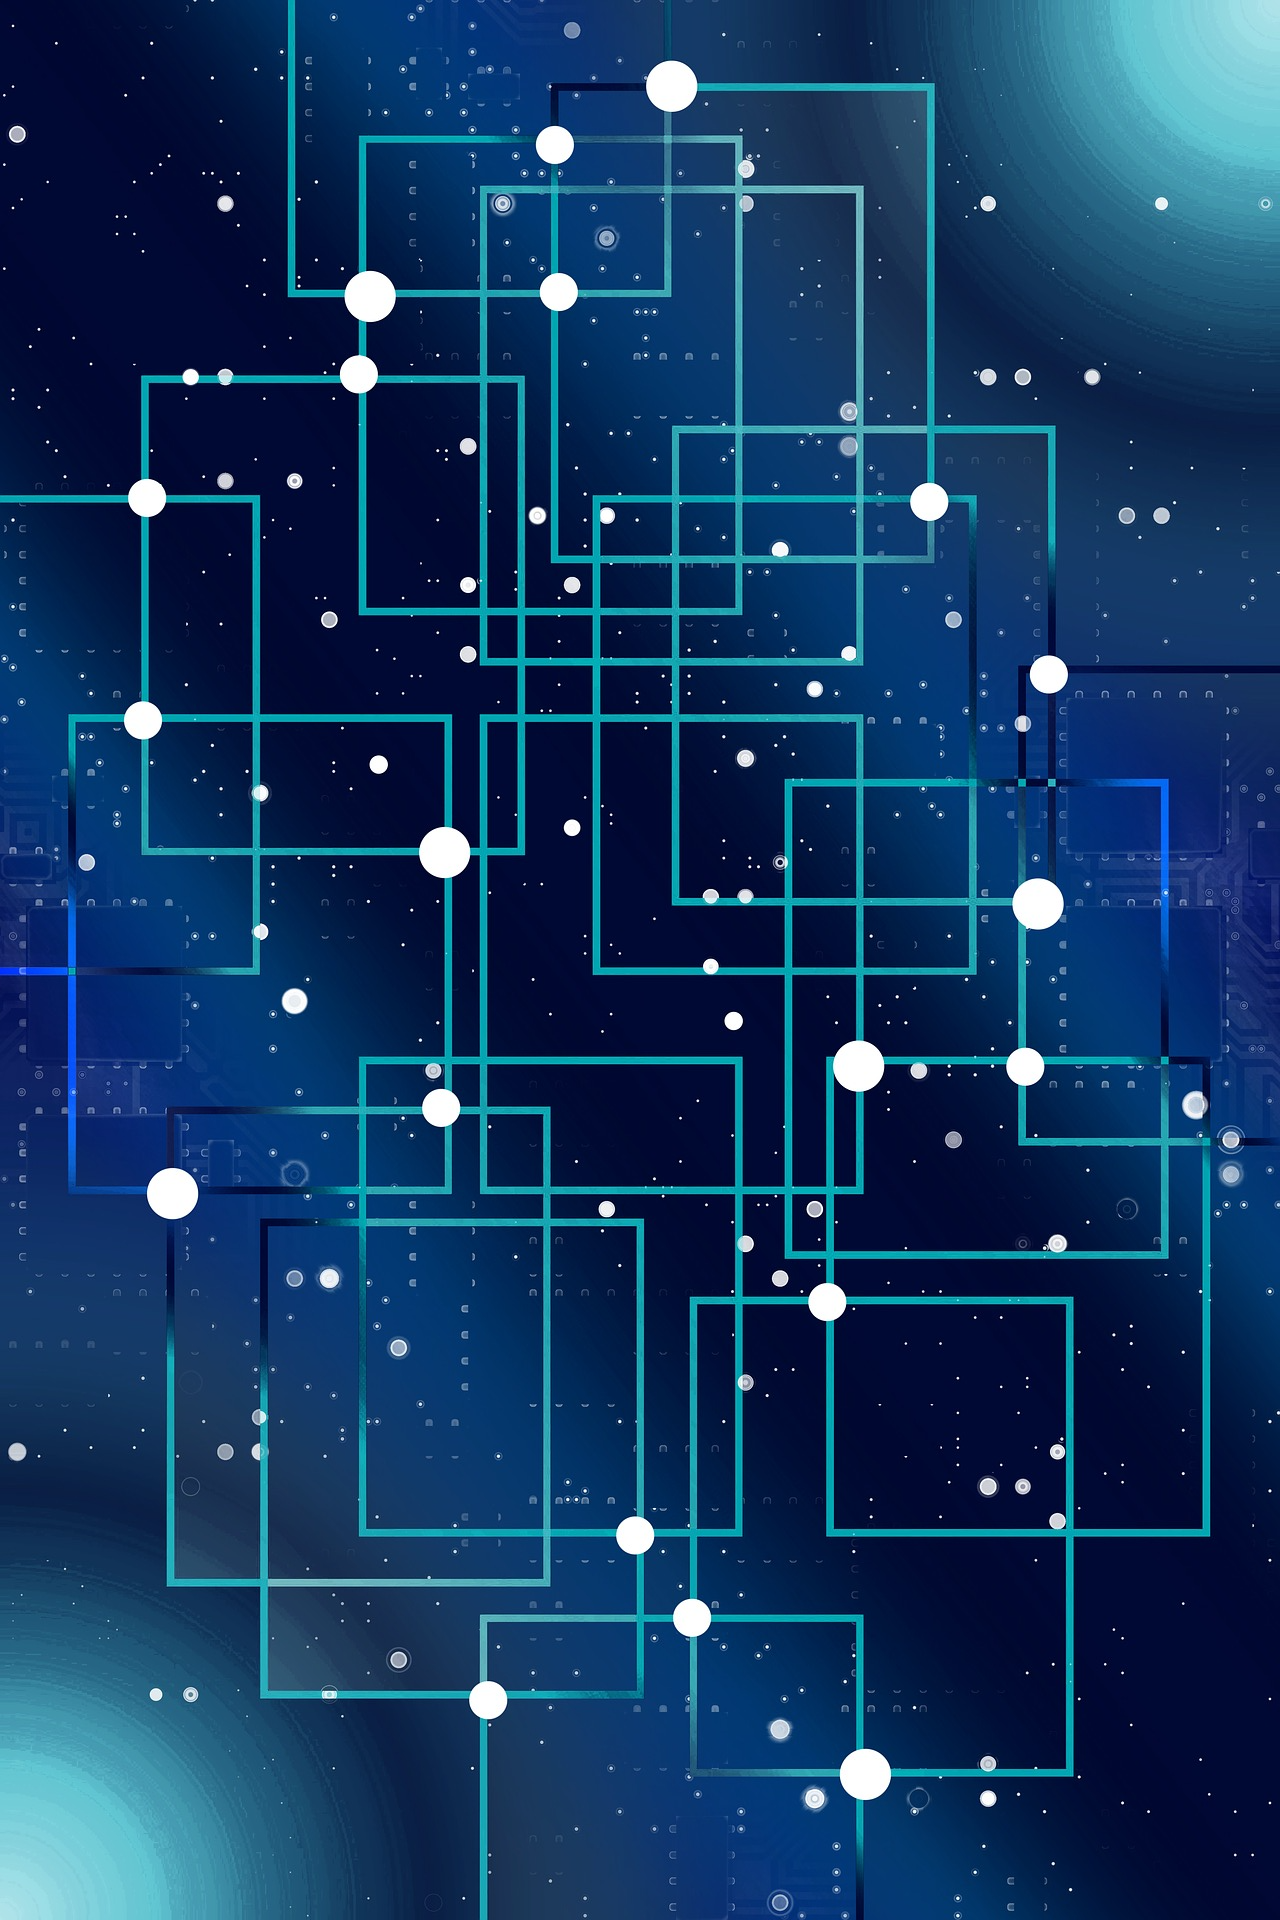
\includegraphics[width=\paperwidth]{background.png}};
\draw (current page.center) node [fill=blue!2!white,fill
opacity=0.9,text opacity=1,inner
sep=1cm]{\Huge\centering\bfseries\sffamily\parbox[c][][t]{\paperwidth}{\centering
    \TITLE \\[15pt] % Book title
{\Large \SUBTITLE}\\[20pt] % Subtitle
{\huge \AUTHOR \\ \Large \EMAIL }}}; % Author name
\end{tikzpicture}
\vfill
\endgroup

%----------------------------------------------------------------------------------------
%	COPYRIGHT PAGE
%----------------------------------------------------------------------------------------

\newpage
~\vfill
\thispagestyle{empty}

\noindent Copyright \copyright\ 2017 \AUTHOR \\

\noindent \EMAIL \\ % Copyright notice

% \noindent \textsc{Indiana University}\\ % Publisher

\noindent \textsc{https://github.com/cloudmesh/classes}\\ % URL

\begin{comment}
\noindent Licensed under the Creative Commons
Attribution-NonCommercial 3.0 Unported License (the ``License''). You
may not use this file except in compliance with the License. You may
obtain a copy of the License at
\url{http://creativecommons.org/licenses/by-nc/3.0}. Unless required
by applicable law or agreed to in writing, software distributed under
the License is distributed on an \textsc{``as is'' basis, without
  warranties or conditions of any kind}, either express or
implied. See the License for the specific language governing
permissions and limitations under the License.\\ % License information

\end{comment}

\noindent \textit{First printing, October 2017} % Printing/edition date

%----------------------------------------------------------------------------------------
%	TABLE OF CONTENTS
%----------------------------------------------------------------------------------------

%\usechapterimagefalse % If you don't want to include a chapter image, use this to toggle images off - it can be enabled later with \usechapterimagetrue

\chapterimage{TOC.png} % Table of contents heading image

\pagestyle{empty} % No headers

\tableofcontents % Print the table of contents itself

\cleardoublepage % Forces the first chapter to start on an odd page so it's on the right

\pagestyle{fancy} % Print headers again



\newcommand{\FILENAME}{\begin{fileremark}\currfiledir
    \currfilename\end{fileremark}}
\newcommand{\CHANGE}{\begin{changeremark}THIS WILL CHANGE
    \currfilename\end{changeremark}}
\newcommand{\TODO}[1]{\todo[inline]{#1}}
\newcommand{\DONE}[1]{DONE: \todo[inline,color=green!30]{#1}}

\newcommand{\FIGURE}[5]{
\begin{figure}[#1] 
  \centering 
    \includegraphics[width=#2\columnwidth]{#3} 
  \caption{#4}\label{#5} 
\end{figure} 
}

\newcommand{\URL}[1]{ \begin{itemize} \item \url{#1} \end{itemize} }
\newcommand{\HREF}[2]{ \begin{itemize} \item \href{#1}{#2} \end{itemize} }

\newcommand{\video}[4]{%
{\em \hfill \href{#4}{#3 (#2)~
\includegraphics[width=\baselineskip]{images/video.png} }}    \index{Video!#1!#3 (#2)}
}

\newcommand{\slides}[4]{%
  {\em  \hfill \href{#4}{#3 (#2)~
\includegraphics[width=\baselineskip]{images/slide.png}}} \index{Slides!#1!#3 (#2)}
}

\DefineVerbatimEnvironment{verbatim}{Verbatim}{xleftmargin=.5in}


\definecolor{codegreen}{rgb}{0,0.6,0}
\definecolor{codegray}{rgb}{0.5,0.5,0.5}
\definecolor{codepurple}{rgb}{0.58,0,0.82}
\definecolor{backcolour}{rgb}{0.97, 0.97, 0.97}
 
\lstdefinestyle{code}{
    backgroundcolor=\color{backcolour},   
    commentstyle=\color{codegreen},
    keywordstyle=\color{magenta},
    numberstyle=\tiny\color{codegray},
    stringstyle=\color{codepurple},
    basicstyle=\footnotesize,
    breakatwhitespace=false,         
    breaklines=true,                 
    captionpos=b,                    
    keepspaces=true,                 
    numbers=left,                    
    numbersep=5pt,                  
    showspaces=false,                
    showstringspaces=false,
    showtabs=false,                  
    tabsize=2
}
 
\lstset{style=code}

\newcommand{\WHERE}[2]{\ref{#1}. \nameref{#1} \hfill ~ #2 ~ \pageref{#1}}


\chapterimage{water.png} % Chapter heading image

%----------------------------------------------------------------------------------------
%	PART
%----------------------------------------------------------------------------------------

\part{Preface}

%----------------------------------------------------------------------------------------
%	CHAPTER
%----------------------------------------------------------------------------------------

\chapterimage{water.png} % Chapter heading image

\chapter{Introduction}

\begin{fileremark}chapter/preface/about.tex\end{fileremark}

\section{About}\label{about}

The document is based on selected material published at the following
Web page

\begin{itemize}
\item
  \url{https://cloudmesh.github.io/classes/}
\end{itemize}

It is part of a class taught at Indiana University. The class
communication takes place at:

\begin{itemize}
\item
  \url{https://piazza.com/class/ix39m27czn5uw}
\end{itemize}

The PDF version will be made in future available at 

\begin{itemize}
\item
\url{https://github.com/laszewski/laszewski.github.io/raw/master/papers/vonLaszewski-bigdata.pdf}
\end{itemize}

This PDF document will be updated based on feedback from the students
and once we have now material available. For a more complete set of
information we recommend the students to visit the Web page.

\section{Citation}

The bibtex entry for this document is

\begin{verbatim}
@TechReport{las17handbook,
  author =       {Gregor von Laszewski},
  title =        {Handbook of Big Data Applications and Analytics},
  institution =  {Indiana University},
  year =         {2017},
  OPTtype =      {Draft},
  address =      {Smith Research Center, Bloomington, IN 47408},
  month =        dec,
  url={https://github.com/laszewski/laszewski.github.io/raw/master/papers/vonLaszewski-bigdata.pdf},
}
\end{verbatim}

\section{Contributors}

We like to acknowledge the following contributors that helped on this
document. Please notify us with your name and a brief commend on what
you contributed:

\begin{description}
\item[John Doe] He contributed to none of teh sections as this is just
  an example.
\end{description}

%----------------------------------------------------------------------------------------
%	PART
%----------------------------------------------------------------------------------------

\part{Documenting Scientific Research}

%----------------------------------------------------------------------------------------
%	CHAPTER 1
%----------------------------------------------------------------------------------------

\chapterimage{writing.png} % Chapter heading image

\chapter{Documenting Scientific Research}
\FILENAME

\section{Writing a Scientific Article or Conference Paper}
\index{Writing}

An important part of any scientific research is to document it. This is
often done through scientific conferences or journal articles. Hence it
is important to learn how to prepare and submit such papers. Most
conferences accept typically the papers in PDF format but require the
papers to be prepared on MSWord or in LaTeX. While working with many
students in the past we noticed however that those students using Word
often spend unnecessarily countless hours on trying to make there papers
beautiful while actually violating the template provided by the
conference. Furthermore, we noticed that the same students had issues
with bibliography management. Instead of Word helping the student it
provided the illusion to be easier than LaTeX but when adding up the
time spend on the paper we found that LaTeX actually saved time. This
has been especially true with the advent of collaborative editing
services such as sharelatex \cite{www-sharelatex} and overleaf
\cite{www-overleaf}. 

In this section we provide you with a professional template that is used
for either system based on the ACM standard that you can use to write
papers. Naturally this will be extremely useful if the quality of your
research is strong enough to be submitted to a conference. We structure
this section as follows. Although we do not recommend that you use
MSWord for your editing of a scientific paper, we have included a short
section about it and outline some of its pitfalls that initially you may
not think is problematic, but has proven to be an issue with students.
Next we will focus on introducing you to LaTeX and showcasing you the
advantages and disadvantages. We will dedicate an entire section on
bibliography management and teach you jhow to use jabref which clearly
has advantages for us.

Having a uniform report format not only helps the students but allow
allows the comparison of paper length and effort as part of teaching a
course. We have added an entire section to this chapter that discusses
how we can manage a \emph{Class Proceedings} form papers that are
contributed by teams in the class.

\subsection{Professional Paper Format}\label{professional-paper-format}

The report format we suggest here is based on the standard ACM
proccedings format. It is of very high quality and can be adapted for
your own activities. Moreover, it is possible to use most of teh text to
adapt to other formats in case the conference you intend to submit your
paper to has a different format. The ACM format is always a good start.

Important is that you do not need to change the template but you can
change some parameters in case you are not submitting the paper to a
conference but use it for class papers. Certainly you should not change
the spacing or the layout and instead focus on writing content. As for
bibliography management we recommend you use jabref which we will
introduce in Section \ref{??}.

We recommend that you carefully study the requirements for the report
format. We would nat want that your paper gets rejected by a journal,
conference or the class just because you try to modify the format or do
not follow the established publication guidlines.

The template we are providing is available from:

\URL{https://github.com/cloudmesh/classes/tree/master/docs/source/format/report}

Convenient compressed files are available at

\URL{https://github.com/cloudmesh/classes/tree/master/docs/source/format/report.tar.gz}
\URL{https://github.com/cloudmesh/classes/tree/master/docs/source/format/report.zip}

You will find in it a modified ACM proceedings templates for Word and
for LaTeX that has an identification box removed on the lower left hand
side of the first page. This is done for classes so that you have more
space to write. In case you must submit to a conference you can use the
original ACM template. This template can be found at

\subsection{Submission Requirements}\label{submission-requirements}

Although the initial requirement for some conferences or journals is the
document PDF, in many cases you must be prepared to provide the source
when submitting to the conference. This includes the submission of the
original images in an images foder. You may ba asked to package the
document into a folder with all of its sources and submit to the
conference for professional publication.

\subsection{Microsoft Word vs. \LaTeX}\label{microsoft-word}

Microsoft word will provide you with the initial impression that you
will safe lots of time writing in it while you see the layout of the
document. This will be initially true, but once you progress to the
more challenging parts and later pages such as image menagement and
bibliography management you will see some issues. Thes include that
figure placement in Word need sto be done just right in order for images
to be where they need. We have seen students spending hours with the
placement of figures in a paper but when they did additional changes the
images jumped around and were not at the place where teh students
expected them to be. So if you work with images, make sure you
understand how to place them. Also always use relative caption counters
so that if an image gets placed elsewhere the counter stays consistent.
So nefer use just the number, but a reference to the figure when referring
to it. Recently a new bibliography management system was added to Word.
However, however it is not well documented and the references are placed
in the system bibliography rather than a local managed bibliography.
This mah have severe consequences when working with many authors on a
paper. The same is true when using Endnote. We have heard in many
occasions that the combination of endnote and Word destroyed documents.
You certainly do not want that to happen the day before your deadline.
Also in classes we observed that those using LaTeX deliver better
structured and written papers as the focus is on text and not beautiful
layout.

For all these reasons we do not recommend that you use Word.

In LaTeX where we have an easier time with this as we can just ignore
all of these issues due to relative good image placement and excellent
support for academic reference management. Hence, it is in your best
interest to use LaTeX. The information we provide here will make it easy
for you to get started and write a paper in no time as it is just like
filling out a form.

\subsection{Working in a Team}\label{working-in-a-team}

Today research is done in potentially large research teams. This also
include the writing of a document. There are multiple ways this is done
these days and depends on the system you chose.

In MSWord you can use skydrive, while for LaTeX you can use sharelatex
and overleaf. However, in many cases the use of github is possible as
the same groups that develop the code are also familiar with github.
Thus we provide you here also with the introduction on how to write a
document in github while group members can contribute.

Here are the options:

\begin{description}

\item [LaTeX and git:] This option will likely safe you time as you can use
  jabref also for managing collaborative bibliographies and
\item [sharelatex:] an online tool to write latex documents
\item [overleaf:] an online tool to write latex documents
\item [MS onedrive:] It allows you to edit a word document in collaboration.
  We recommend that you use a local installed version of Word and do the
  editing with that, rather than using the online version. The online
  editor has some bugs. See also (untested):
  \url{http://www.paulkiddie.com/2009/07/jabref-exports-to-word-2007-xml/},
  \url{http://usefulcodes.blogspot.com/2015/01/using-jabref-to-import-bib-to-microsoft.html}
\item [Google Drive:] google drive could be used to collaborate on text that
  is than pasted into document. However it is just a starting point as
  it does not support typically the format required by the publisher.
  Hence at one point you need to swithc to one of the other systems.
\end{description}

\subsection{Timemanagement}\label{timemanagement}

Obviously writing a paper takes time and you need to car-fully make sure
you devote enough time to it. The important part is that the paper
should not be an after thought but should be the initial activity to
conduct and execute your research. Remember that

\begin{enumerate}

\item  It takes time to read the information
\item  It takes time understand the information
\item  It takes time to do the research

\end{enumerate}

For deadlines the following will get you in trouble:

\begin{enumerate}

\item
  \emph{There are still 10 weeks left till the deadline, so let me start
  in 4 week \ldots{}}. Procrastination is your worst enemy.
\item
  If you work in a team that has time management issues address them
  immediately
\item
  Do not underestimate the time it takes to prepare the final submission
  into the submission system. Prepare automated scripts that can deliver
  the package for submission in minutes rather than hours by hand.
\end{enumerate}

\subsection{Paper and Report Checklist}\label{paper-checklist}
\index{Writing!Checklist}

In this section we summarize a number of checks that you may perform to
make sure your paper is properly formatted and in excellent shape.
Naturally this list is just a partial list and if you find things we
should add here, let us know.

\begin{itemize}[label=$\Box$]

\item Have you written the report in the specified format?

\item Have you included an acknowledgement section?

\item Have you included the paper in the submission system (In our
  case git). This includes all images, bibliography files and other
  material that is needed to build the paper from scratch?

\item Have you added the bibliography file that you managed (In our
  case jabref to make it simple for you)?

\item Have you specified proper identification in the submission
  system for your submission.  This is typically a form or ASCII text
  that needs to be filled out and follows a very particular format.
  In our case it is a README.md file that ncludes a homework ID, names
  of the authors, and e-mails)?

\item In case you used word have you also provided the jabref?

\item In case of a class and if you do a multi-author paper, have you
  added a work-breakdown section in the appendix describing who did
  what in the paper?

\item IN case you have an appenix it is included fater the bibliography

\item Have you spellchecked the paper?

\item Have you grammar chacked the paper?

\item Are you using \textbf{a} and \textbf{the} properly?

\item Have you made sure you do not plagiarize?

\item Is the title properly capitalized?

\item Have you not used phrases such as shown in the Figure below, but
  instead used as shown in Figure 3 when referring to the 3rd figure?
  Numbers in LaTeX are done with \verb|\label{}| after captions and
  \verb|\ref{}| in the text (See examples in the LaTeX section). In
  word you must use relative numbering.

\item Have you capitalized ``Figure 3'', ``Table 1''?

\item Have you removed any figure that is not referred explicitly in
  the text. E. ech figure needs a text such as  {\em As shown in
    Figure ..} or similar.

\item Are the figure captions bellow the figures and not on top. (Do
  not include the titles of the figures in the figure itself but
  instead use the caption or that information?

\item When using tables have you put the table caption above the table?

\item When using image have you put the table caption bellow the image?

\item Make the figures large enough so we can read the details. If
  needed make the figure over two columns? 

\item Do not worry about the figure placement if they are at a
  different location than you think. Figures are allowed to float. In
  many submissions you may have to place all figures at the end of the
  paper so you can focus on content rather than placing figures. In
  addition it will help you to refer to the figures by index.

\item Are all figures and tables at the end?

\item In case you copied a figure from another paper you need to ask
  for copyright permission. In case of a class paper you \textbf{must}
  include a reference to the original at the end of the figure caption.

\item Do not use the word ``I'' instead use ``we'' even if you are the
  sole author.

\item Do not use the phrase ``In this paper/report we show'' instead
  use ``We show''. It is not important if this is a paper or a report
  and does not need to be mentioned.

\item Do not artificially inflate your paper if you are bellow the
  page limit and have nothing to say anymore.

\item If your paper limit is 12 pages but you want to hand in 120
  pages, please check first ;-) If your page limoit is 2 pages but you
  hand in 4 thats is no issue.

\item Do not use the characters \& \# \% \_  in the paper if you use
  LaTeX. If you use them you probably need a bakslash in front of them.

\item Latex uses double single open quotes and double single closed
  quotes for quotes. Have you made sure you replaced them?

  When using quotes in LaTeX, do not use the double quote but instead
  use two single quotes such as \verb|``This is a quote''|. THis will
  place the proper quotes in the text. To only use the quotes when you
  literraly quote from other papers. Never use a quote to emphasize a
  thext. For that you use \verb|{\em this is emphasize}| resulting in
  {\em This is emphasized}.

\item If you want to say and do not use \& but use the word {\em
    and}. If you need tou use it be reminded to write it as \verb|\&|


\item Pasting and copying from the Web often results in non ascii
  characters to be used in your text, please remove them and replace
  accordingly. This includes some form of -- that you may see showing
  up as fi in pdf

\item Is your Abstract not a proposal? Abstracts are no proposals, e.g
  This paper intends to show .... If the paper intends to show you are
  still in the draft phase of the paper. However, if you say We sow
  ... That would be good. Let us just assume you intended to show
  something but did not achieve then you can say We intended to show
  this but we showed it was not possible. As you can see not only the
  intention is communicated, but the result. If you just focuss on the
  intent that's just a proposal and is not a proper abstract.

\item Are you not using the word paper in your writeup?  Abstracts and
  the entire paper should not have the word paper in it.

\item If your paper is an introduction or overview paper, please do
  not assume the reader to be an expert. Provide enough material for
  the paper to be useful for an introduction into the topic. 

\item Are you refernces correct? References to a paper are no
  afterthought, they should be properly cited. Use jabref and make
  sure the citation type of the refernce is correct and fill out as
  many fields as you can. Some jouranls and conferences have for
  example special requirements that go beyond the requirements of for
  example jabref. One example is that maky conferences require you
  that wne you cite papers form another conference to augment the
  conferences not only with the location where the conference took
  place, but also with the dates the conference took
  place. Unfortunately, this is information that is often only
  avalable through additional google quesies and many refernce entries
  you find in the internet do not have this information readily
  available.

\end{itemize}

In case of a class

\begin{itemize}[label=$\Box$] 

\item Check in your current work of the paper on a weekly basis to
  show consistent progress.

\item Please use the dedicated report format for class. It may not be
  the ACM or IEEE format, but may have some additions that make
  management of bibliographies easier. Do follow our instructions for
  bibliographies.

\end{itemize}

In case you are allowed to use word in class, such as the one we teach
at IU, the following applies in addition:

\begin{itemize}[label=$\Box$] 

\item Are you managing your references in jabref and endnote (we need
  both)
\item Are you using the right template we have a special 2 column
  template for the class that is a modified version from the 2 column
  ACM template
\item Are you using build in numbered section management? MSWord has
  Sections that must be used
\item Are you using real bulleted lists in Word and not just a ``*''
  or a ``-''?
\item Have you carelessly pasted and copied into the document without
  using proper formats. E.g. in MSWord this is a problem. You need to
  fix the format and use the build in format. Not that if you paste
  wrong you effect the format styles.
\item Have you created not only a docx document but also the PDF.

\item Make sure you use .docx and not .doc

\end{itemize}

If you observe something missing let us know.

\subsection{Example Paper}\label{example-paper}

An example report in PDF format is available:

\begin{itemize}

\item
  \href{https://github.com/cloudmesh/classes/blob/master/docs/source/format/report/latex/report.pdf}{report.pdf}
\end{itemize}

\subsection{Creating the PDF from LaTeX on your
Computer}\label{creating-the-pdf-from-latex-on-your-computer}

Latex can be easily installed on any computer as long as you have
enough space. Furthermore if your machine can execute the make command
we have provided in the standard report format a simple
\href{https://github.com/cloudmesh/classes/blob/master/docs/source/format/report/latex/Makefile}{Makefile}
that allows you to do editing with immediate preview as documented in
the LaTeX lesson.

\subsection{Class Specific README.md}\label{class-specific-readme.md}

For the class we will manage all papers via github.com. You will be
added to our github at

\URL{https://github.com/bigdata-i523}

and assigned an hid (homework index directory) directory with a unique
hid number for you. In addition, once you decide for a project, you will
aslso get a project id (pid) and a directory in which you place the
projects. Projects must not be placed in hid directories as they are
treated differently and a class proceedings is automatically created
based on your submission.

As part of the hid directory, you will need to create a README.md file
in it, that \textbf{must} follow a specific format. The good news is
that we have developed an easy template that with common sense you can
modify easily. The template is located at

\URL{https://raw.githubusercontent.com/bigdata-i523/sample-hid000/master/README.md}

As the format may have been updated over time it does not hurt to
revisit it and compare with your README.md and make corrections. It is
important that you follow the format and not eliminate the lines with
the three quotes. The text in the quotes is actually yaml. yaml is a
data format the any data scientist must know. If you do not, you can
look it up. However, if you follow our rules you should be good. If you
find a rule missing for our purpose, let us know. We like to keep it
simple and want you to fill out the \emph{template} with your
information.

Simple rules:

\begin{itemize}

\item
  replace the hid nimber with your hid number.
\item naturally if you see sample- in the directory name you need to

  delete that as your directory name does not have sample- in it.
\item do not ignore where the author is to be placed, it is in a list

  starting with a -
\item there is always a space after a -

\item do not introduce empty lines

\item do not use TAB and make sure your editor does not bay accident

  automatically creates tabs. This is probably the most frequent error
  we see.
\item do not use any : \& \_ in the attribute text including titles

\item an object defined in the README.md must have on a single type

  field.  for example in the project section. Make sure you select
  only one type and delete the other
\item in case you have long paragraphs you can use the \textgreater{}

  after the abstract
\item Once you understood how the README.md works, please delete the

  comment section.
\item Add a chapter topic that your paper belongs to

\end{itemize}

\subsection{Exercise}\label{exercise}

\begin{description}
\item[Report.1:]
Install latex and jabref on your system
\item[Report.2:]
Check out the report example directory. Create a PDF and view it. Modify
and recompile.
\item[Report.4:]
Learn about the different bibliographic entry formats in bibtex
\item[Report.5:]
What is an article in a magazine? Is it really an Article or a Misc?
\item[Report.6:]
What is an InProceedings and how does it differ from Conference?
\item[Report.7:]
What is a Misc?
\item[Report.8:]
Why are spaces, underscores in directory names problematic and why
should you avoid using them for your projects
\item[Report.9:]
Write an objective report about the advantages and disadvantages of
programs to write reports.
\item[Report.10:]
Why is it advantageous that directories are lowercase have no underscore
or space in the name?
\end{description}

% \begin{fileremark}\url{https://github.com/cloudmesh/classes/blob/master/docs/source/lesson/doc/report.rst}\end{fileremark}
\section{Report Format}\label{report-format}

Although we provide \textbf{trivial} but detailed report format
requirements, we observed over the years that some students still asked
us can I make my report shorter, or can i use a different format? The
answer to these questions is \textbf{no}. Furthermore, we observed that
the same students than went ahead and played with the formating and
introduced empty lines, increased tables or figures, or worse modified
the fontsize to circumvent the page limit requirement.

Thus we have adopted a much simpler approach that is easy to summarize

\begin{enumerate}
\def\labelenumi{\arabic{enumi}.}
\tightlist
\item
  We provide you with a \textbf{high quality} report template format
  that you must not change and is used by millions of researchers.
\item
  All references must be managed with jabref as reference management
  tool and must be provided in addition to the document.
\item
  If your document does not follow the format or we find that you have
  modified the style of the template we provide will return the document
  without review.
\item
  It is in the students responsibility to use the template format from
  the beginning on. In fact, our assignments will use the template for
  all assignments and not just your term paper or term report.
\end{enumerate}

The template for the report is available from:

\begin{itemize}
\tightlist
\item
  \url{https://github.com/cloudmesh/classes/tree/master/docs/source/format/report}
\end{itemize}

Convenient compressed files are available at

\begin{itemize}
\tightlist
\item
  \url{https://github.com/cloudmesh/classes/tree/master/docs/source/format/report.tar.gz}
\item
  \url{https://github.com/cloudmesh/classes/tree/master/docs/source/format/report.zip}
\end{itemize}

You have two choices. A good one and a bad one.

The good choice is to use the LaTeX template and write your document in
LaTeX. The bad one is to use the Word template and write the document in
Word. Both templates are included in our git repository.

Hence, it is in your best interest to use LaTeX. The good news is that
we have made it simple for you to use it. Furthermore, you are allowed
to use online services. An example report in PDF format is available:

\begin{itemize}
\tightlist
\item
  \href{https://github.com/cloudmesh/classes/blob/master/docs/source/format/report/latex/report.pdf}{report.pdf}
\end{itemize}

We provide a very simple
\href{https://github.com/cloudmesh/classes/blob/master/docs/source/format/report/latex/Makefile}{Makefile}
that allows you to do editing with immediate preview as documented in
the LaTeX lesson. Due to LaTeX being a \textbf{trivial} ASCII based
format and having a superior bibliography management you will save
yourself many hours of work that you will face while fighting with Word.
We got feedback from those that tried it and they thanked us later.
Furthermore, in case you are in a team, you can use either git while
collaboratively developing the LaTeX document, use sharelatex, or
overleaf.

However, we allow you to use word under the following conditions:

\begin{enumerate}
\def\labelenumi{\arabic{enumi}.}
\tightlist
\item
  You accept the risk that Word may crash and you may find yourself in
  last minute in the situation that you lost your work and your document
  is broken. We will not be sympathetic to this situation as we
  recommended that you use LaTeX.
\item
  You must use not only Endnote, but also jabref when managing your
  references, so you have to do the management of references twice. This
  is so that your document could be converted to LaTeX in case we think
  it suitable for publication in a conference or workshop.
\item
  You do not modify the theme.
\item
  All images and tables are placed at the end of the paper.
\item
  Git wil be used to submit all documents with regular updates.
\end{enumerate}

For LaTeX you will encounter a much more smooth experience.

\begin{enumerate}
\def\labelenumi{\arabic{enumi}.}
\tightlist
\item
  Your final document must be committed in git and as LaTeX is ASCII
  based you can do thous throughout the semester and have backups via
  git.
\item
  You will be using jabref to manage your bibliography and as LaTeX has
  build in support for bibliography management there is not much you
  need to pay attention to, all Format of the references is done for you
  in case you entered them correctly
\item
  You do not modify our theme.
\item
  All images and tables are placed at the end of the paper.
\item
  Git wil be used to submit all documents.
\item
  You are allowed to use sharelatex or overleave so you do not have to
  install LaTeX on your computer, but see 5. and the next paragraph.
\end{enumerate}

Whatever format you use, your final submission must be in \textbf{the
class} git. We will not review any documents stored on sharelatex or
overleaf or in any git repository not belonging to the class. Your final
submission will include the bibliography file(s) as a separate
document(s). All images must be placed in an images folder and submitted
in your repository with the originals. When using sharelatex or overleaf
you must replicate the directory layout carefully from our template and
include your final documents in git with a Makefile that can recreate
the document. It is in your responsibility that this works. We will
regenerate the document from source before we grade it. Thus it is not
sufficient to just check in the final PDF. The report must be spell
checked.

\begin{description}
\item[There will be \textbf{NO EXCEPTION} to this. We will not]
review your report if its submission is incomplete.
\end{description}

\subsection{Leverage parallel editing}\label{leverage-parallel-editing}

In most cases you will be able to work in groups on class projects. This
allows you to develop the report collaboratively. Here are some options:

\begin{enumerate}
\tightlist
\item
  LaTeX and git: THis option will likely safe you time as you can use
  jabref also for manageing collaborative bibliographies and
\item
  MS onedrive: It allows you to edit a word document in collaboration.
  We recommend that you use a local installed version of Word and do the
  editiong with that, rather than useing the online verison. The online
  editor has some bugs. See also (untested):
  \url{http://www.paulkiddie.com/2009/07/jabref-exports-to-word-2007-xml/},
  \url{http://usefulcodes.blogspot.com/2015/01/using-jabref-to-import-bib-to-microsoft.html}
\item
  Google Drive: google drive could be used to collaborate on text that
  is than pasted into document. he final document will not accept as
  google document. You must use the 2 column ACM template. We observed
  that students that use google docs lack structure and we no longer
  allow it as final document format. It also does not allow us to
  uniformly compare the documents between each other. It is easy to
  transfer it to LaTeX.
\end{enumerate}

\subsection{Timemanagement Tips}\label{timemanagement-tips}

Obviously taking a class takes time

\begin{enumerate}
\tightlist
\item
  It takes time to read the information
\item
  It takes time understand the information
\item
  It takes time to do the project
\item
  This will get you in trouble: \emph{There are still 10 weeks left till
  the project is due so let me start in 4 weeks \ldots{}}. Postponing
  the project till the last moment
\item
  Do not spend significant time on unimportant documentation and setup.
  Instead spend time to develop cmd5 comamnds and scripts that do these
  things automatically
\end{enumerate}

\subsection{Report Checklist}\label{report-checklist}

This partiald list may serve as a way to check if you follow the rules

\begin{enumerate}
\tightlist
\item
  Have you written the report in the specified format?
\item
  Have you included an acknowledgement section?
\item
  Have you included the report in git?
\item
  Have you specified the HID, names, and e-mails of all team members in
  your report. E.g. the Real Names that are registered in Canvas?
\item
  Have you included the project number in the report?
\item
  Have you included all images in native and PDF format in git in the
  images folder?
\item
  Have you added the bibliography file that you managed with jabref
\item
  In case you used word have you also provided the endnote file
\item
  Have you added an appendix describing who did what in the project or
  report?
\item
  Have you spellchecked the paper?
\item
  Are you useing \textbf{a} and \textbf{the} properly?
\item
  Have you made sure you do not plagiarize?
\item
  Have you not used phrases such as shown in the Figure below, but
  instead used as shown in Figure 3 when referring to the 3rd figure?
\item
  Have you capitalized ``Figure 3'', ``Table 1'', \ldots{} ?
\item
  Any figure that is not referred to explicitly in the text must be
  removed.
\item
  Are the figure captions bellow the figures and not on top. (Do not
  include the titles of the figures in the figure itself but instead use
  the caption or that information?
\item
  When using tables have you put the table caption on top?
\item
  Make the figures large enough so we can read the details. If needed
  make the figure over two columns?
\item
  Do not worry about the figure placement if they are at a different
  location than you think. Figures are allowed to float. If you want you
  can place all figures at the end of the report?
\item
  Are all figures and tables at the end?
\item
  Do not use the word ``I'' instead use we even if you are the sole
  author?
\item
  Do not use the phrase ``In this paper/report we show'' instead use
  ``We show''. It is not important if this is a paper or a report and
  does not need to be mentioned.
\item
  Do not artificially inflate your report if you are bellow the page
  limit and have nothing to say anymore.
\item
  If your paper limit is 12 pages but you want to hand in 120 pages,
  please check first with an instructor ;-)
\item
  Check in your current work of the report on a weekly basis to show
  consistent progress.
\item
  Please use the dedicated report format for class. It may not be the
  ACM or IEEE format, but may have some additions that make management
  of bibliographies easier. Do follow our instructions for
  bibliographies.
\item
  Do not use the characters \& \# \% in the paper if you use LaTeX. If
  you use them you prabably need a in front of them.
\item
  If you want to say and do not use \& but use the word and.
\item
  (I524) Is in your report directory a README.rst file in it as shown in
  the example project that we introduced you to?
\item
  (I523) you do not have to place a readme in your report or paper
  directories. Instead create a README.md in your hid or pid
  directories.
\end{enumerate}

If you observe something missing let us know.

In case you are allowed to use word The following applies in addition

\begin{enumerate}
\tightlist
\item
  Are you manageing your refernces in jabref and endnote (we need both)
\item
  Are you using the right template we have a special 2 column template
  for the class that is a modified version from the 2 column ACM
  template
\item
  Are you using build in numbered section management? MSWord has
  Sections that must be used
\item
  Are you using real bulleted lists in Word and not just a ``*'' or a
  ``-''?
\item
  Have you carelessly pasted and copied into the document without using
  proper formats. E.g. in MSWord this is a problem. You need to fix the
  format and use the build in format. Not that if you paste wrong you
  effect the format styles.
\item
  Have you created not only a docx document but also the PDF.
\item
  Make sure you use .docx and not .doc
\end{enumerate}

If you have other things to add, send them via piazza and we will add
them here.

\subsection{README.md}\label{readme.md}

For I523, Fall 2017, we will manage all papers via github.com. You will
be added to our github at

\begin{itemize}
\tightlist
\item
  \url{https://github.com/bigdata-i523}
\end{itemize}

and assigned an hid (homework index directory) directory with a unique
hid number for you. In addition, once you decide for a project, you will
aslso get a project id (pid) and a directory in which you place the
projects. Projects must not be placed in hid directories as they are
treated differently and a class proceedings is automatically created
based on your submission.

As part of the hid directory, you will need to create a README.md file
in it, that \textbf{must} follow a specific format. The good news is
that we have developed an easy template that with common sense you can
modify easily. The template is located at

\begin{itemize}
\tightlist
\item
  \url{https://raw.githubusercontent.com/bigdata-i523/sample-hid000/master/README.md}
\end{itemize}

As the format may have been updated over time it does not hurt to
revisit it and compare with your README.md and make corrections. It is
important that you follow the format and not eliminate the lines with
the three quotes. The text in the quotes is actually yaml. yaml is a
data format the any data scientist must know. If you do not, you can
look it up. However, if you follow our rules you should be good. If you
find a rule missing for our purpose, let us know. We like to keep it
simple and want you to fill out the \emph{template} with your
information.

Simple rules:

\begin{itemize}
\tightlist
\item
  replace the hid nimber with your hid number.
\item
  naturally if you see sample- in the directory name you need to delete
  that as your directory name does not have sample- in it.
\item
  do not ignore where the author is to be placed, it is in a list
  starting with a -
\item
  there is always a space after a -
\item
  do not introduce empty lines
\item
  do not use TAB and make sure your editor does not bay accident
  automatically creates tabs. This is probably the most frequent error
  we see.
\item
  do not use any : \& \_ in the attribute text including titles
\item
  an object defined in the README.md must have on a single type field.
  for example in the project section. Make sure you select only one type
  and delete the other
\item
  in case you have long paragraphs you can use the \textgreater{} after
  the abstract
\item
  Once you understood how the README.md works, please delete the comment
  section.
\end{itemize}

\subsection{README.rst (for I524, Spring
2017)}\label{readme.rst-for-i524-spring-2017}

In the directory that containes the report, please include the following
README.rst file. Without this file we will not review your document:

\begin{verbatim}
Title: The title of your paper (one line)

Author: The author s of the paper (one line)

HID: The HID of the authors in the order as specified in authors (one line)

PID: The PID of the paper (there will be exactly one)

E-mail: The e-mails of the authors in the order of the author list (one line)

Format: latex or word (specify one)
\end{verbatim}

Please note that all information has an empty line between them and all
information is stored in one line

This information is used to autogenerate the class proceedings.

\subsection{Exercise}\label{exercise}

\begin{description}
\item[Report.1:]
Install latex and jabref on your system
\item[Report.2:]
Check out the report example directory. Create a PDF and view it. Modify
and recompile.
\item[Report.4:]
Learn about the different bibliographic entry formats in bibtex
\item[Report.5:]
What is an article in a magazine? Is it really an Article or a Misc?
\item[Report.6:]
What is an InProceedings and how does it differ from Conference?
\item[Report.7:]
What is a Misc?
\item[Report.8:]
Why are spaces, underscores in directory names problematic and why
should you avoid using them for your projects
\item[Report.9:]
Write an objective report about the advantages and disadvantages of
programs to write reports.
\item[Report.10:]
Why is it advantageous that directories are lowercase have no underscore
or space in the name?
\end{description}


\chapter{Introduction to \LaTeX}

\begin{fileremark}
\url{chapter/doc/latex.tex}\end{fileremark}

Mastering a text processing system is an essential part of a
researcher's life. Not knowing how to use a text processing system can
slow down the productivity of research drastically.

\section{Installation}
\label{installation}
\index{Latex!installation}

LaTeX is available on all modern computer systems. A very good
installation for OSX is available at:

\begin{itemize}
\tightlist
\item
  \url{https://tug.org/mactex/}
\end{itemize}

However, if you have older versions on your systems you may have to
first completely uninstall them.

\subsection{Local Install}\label{local-install}

Installing LaTeX is trivial, and is documented on the internet very
well. However, it requires sufficient space and time as it is a large
environment. A system such as TeX Live takes in full install about 5.5
GB. In addition to LaTeX we recommend that you install jabref and use it
for bibliography management.

Thus you will have the most of them on your system.

\begin{itemize}
\tightlist
\item
  pdflatex: the latex program producing pdf
\item
  bibtex: to create bibliographies
\item
  jabref: GUI application to bibtex files (\url{http://www.jabref.org/})
\end{itemize}

Make sure you check that these programs are there, for example with the
Linux commands:

\begin{verbatim}
which pdflatex
which bibtex
which jabref (on OSX you may have an icon for it)
\end{verbatim}

If these commands are missing, please install them. For the newest
documentation on installation of LaTeX we recommend you look up the
installation for your specific OS.

\subsubsection{Install on Ubuntu 16.04}\label{install-on-ubuntu-16.04}
\index{Latex!installation!ubuntu}

The easiest way to install it on ubuntu is to use the terminal and type
in (make sure you have enough space):

\begin{verbatim}
sudo apt-get install texlive-full
\end{verbatim}

One of the best editors for LaTeX is emacs as you can also do
bibliography management with it and not just LaTeX. However, other
editors are available including:

\begin{itemize}
\tightlist
\item
  Kile, TeXworks, JLatexEditor, Gedit LaTeX Plugin, TeXMaker
\end{itemize}

Please look up how to install them if you like to use them. TeXMaker is
popular, However I find the combination of emacs and latexmk superior.
TeXmaker is installed with:

\begin{verbatim}
sudo apt-get install texmaker
\end{verbatim}

Other installations:

\begin{itemize}
\tightlist
\item
  kile is installed by default
\item
  \url{https://www.tug.org/texworks/} (Works on ubuntu, Windows, OSX)
\end{itemize}

\subsubsection{LaTeX for OSX}\label{latex-for-osx}
\index{Latex!installation!OSX}

\begin{itemize}
\tightlist
\item
  \url{https://www.latex-project.org/get/}
\end{itemize}

\subsubsection{LaTeX for Windows}\label{latex-for-windows}
\index{Latex!installation!Windows}

\begin{itemize}
\tightlist
\item
  \url{https://www.latex-project.org/get/}
\end{itemize}

\subsection{Online Services}\label{online-services}

\subsubsection{Sharelatex}\label{sharelatex}
\index{Latex!Sharelatex}

ShareLaTeX is an online, collaborative LaTeX editor that makes the
creation, preview, and sharing of LaTeX documents easy through a
web-based interface.  Those that like to use latex, but do not have it
installed on their computers may want to look at the following video:

Video: \url{https://youtu.be/PfhSOjuQk8Y}

Video with cc: \url{https://www.youtube.com/watch?v=8IDCGTFXoBs}

ShareLaTeX not only allows you to edit online, but allows you to share
your documents in a group of up to three. Licenses are available if you
need more than three people in a team.

\paragraph{IU Licensed ShareLaTeX}

At IU we has a license for the ShareLaTeX service available to School
of Informatics and Computing and Engeneering students, faculty, and
staff only on the Bloomington campus.  

You can create a free ShareLaTeX account but the free accounts have
limitations.  Adding your account to the IU license will give you access
to advanced features, including unlimited sharing.  
It will also allow GitHub integration. THis however only works with
the commercial github.com and not the IU Enterprise GitHub at
github.iu.edu. As we require in our courses github.com you will be
able to use it.

{\em Please note that this license is only available to School of
Informatics and Computing students, faculty, and staff on the
Bloomington campus.  Students must be enrolled in one of the SoIC
degree programs on the Bloomington campus to be eligible.  Students in
other degree programs (even those taking SoIC classes) are not
eligible.}


If you want to use this service, please do and be aware of the following: 

\begin{enumerate}

\item Go to the ShareLaTeX site and register.  Please note that you
  {\bf must} use either an \verb|@indiana.edu| or \verb|@iu.edu| email
  address when you register. If you use any other email address, we
  will not be able to add you to our site license.  You are also
  required to use your IU passphrase as your ShareLaTeX password.
  Once you have registered, send an email to
  \verb|soichelp@indiana.edu} asking to have your sharelatex account 
  added to the IU license.  

\item
  In your request, you must include the following: The IU email
  address you used when you registered (which must be in either the
  \verb|@indiana.edu| or \verb|@iu.edu| domain) A statement indicating
  that you understand that the ShareLaTeX service cannot be used for
  any sensitive data

\item Note that the ShareLaTeX service is {\bf not} qualified for any
  sensitive data. This includes all data in the Critical, Restricted,
  and University-Internal categories as defined in the Data
  Classifications Page.

\end{enumerate}


\subsubsection{Overleaf}\label{overleaf}
\index{Latex!overleaf}

Overleaf.com is a collaborative latex editor. In its free version it has
a very limited disk space. However it comes with a Rich text mode that
allows you to edit the document in a preview mode. The free templates
provided do not include ACM template, put you are allowed to use the OSA
template.

Features of overleaf are documented at:
\url{https://www.overleaf.com/benefits}

\subsubsection{Paperia}\label{paperia}

We do not know where this service is located. However it offers similar
services as ShareLatex and Overleaf.

\begin{itemize}
\tightlist
\item
  \url{https://papeeria.com/}
\end{itemize}


\section{Basic LaTeX Elements}\label{latex}
\index{Latex!Elements}

Often researchers may be initially overwhelmed with all the features
that \LaTeX provides. However, it is much simpler than you initially
believe. In Chapter ?? we introduced you towards using an article
template. As a template is provided you can just look at the elements
in that article and modify or copy them while adapting the
content. Thus, it is more like filling out a form. You do not have to
learn much and you can learn as you go. We are providing in this
chapter some basic \LaTeX elements that will help you getting started
quickly while serving you as a reminder what how to do certain things
in \LaTeX.

\subsection{Characters}\label{characters}

LaTeX is a command language and as such uses some special characters as
part of the language. Thus if you want to use these characters either in
your text or bibliography you need to be especially carful about. These
characters include \% \$ \# \_

Other than in hypreref links and urls you need to put a backslash in
front of them. For example to print a \% in the text you need to use:

\begin{verbatim}
\%
\end{verbatim}

Furthermore tthe character " is not at all used as discussed in the next
section.

\subsection{Highlighting Text}\label{highlighting-text}
\index{Latex!Elements!highlight text}

Quotes are not written with the " character, but are embedded in two
left single quotes and two right single quotes:

\begin{verbatim}
``This is a quote''
\end{verbatim}

which will result in:

``This is a quote''

In many papers we see that the quote is misused while putting quotes
around a word. However quotes are often just used to quote a text from
another paper. Instead of using quotes authors may actually emphasize a
word. LaTeX has a special command for that using:

\begin{verbatim}
{\em this is emphasized}
\end{verbatim}

resulting in

\emph{this is emphasized}

To write a text as bold (which should also be avoided as bold is
typically used in section headers), you can use:

\begin{verbatim}
{\em this is bold fett}
\end{verbatim}

resulting in

\textbf{this is bold fett}

\subsection{Sections}\label{sections}
\index{Latex!Elements!sections}

LaTeX provides a convenient mechanism to structure a paper with sections
and subsections THis is achieved with the following commands:

\begin{verbatim}
\section{This is a Section}
\subsection{This is a Subsection}
\subsubsection{This is a Subsubsection}  
\end{verbatim}

Once you use one of these commands the next paragraph will start bellow
the section command.

In addition you have the command:

\begin{verbatim}
\paragraph{This is a paragraph.}

The line is behind the paragraph heading
\end{verbatim}

The command is special as it does not introduce a new line between the
Heading and the next line even if you include empty lines

\subsection{Empty Lines}\label{empty-lines}

Multiple empty lines will be reduced to a single empty line.

\subsection{Itemize}\label{itemize}
\index{Latex!Elements!itemiz}

Itemized lists can be written as:

\begin{verbatim}
\begin{itemize}
   \item First item
   \item Second item
\begin{itemize}
\end{verbatim}

resulting in

\begin{itemize}
\tightlist
\item
  First item
\item
  Second item
\end{itemize}

\subsection{Enumerate}\label{enumerate}
\index{Latex!Elements!enumerate}

Enumerations can be written as:

\begin{verbatim}
\begin{enumerate}
   \item First item
   \item Second item
\begin{enumerate}
\end{verbatim}

resulting in

\begin{enumerate}
\tightlist
\item
  First item
\item
  Second item
\end{enumerate}

\subsection{Descriptions}\label{descriptions}
\index{Latex!Elements!description}

Description lists can be written as:

\begin{verbatim}
\begin{itemize}
   \item[Cloud] My definition of a Cloud.
   \item[Big Data] My definition of Big Data
\begin{itemize}
\end{verbatim}

\begin{description}
\item[Cloud:]
My definition of a Cloud
\item[Big Data:]
My definition of Big Data
\end{description}

\subsection{Images}\label{images}
\index{Latex!Elements!images}

Figures are extremely easy to handle by including them from source. We
never worry about the placement as LaTeX does typically a very
good job of doing this.:

\begin{verbatim}
In Figure \ref{F:graph} we show a black and white graph about ... .

\begin{figure}
  \includegraphics[width=\columnwidth]{images/graph.pdf}
  \caption{A sample black and white graphic. \cite{las17graph}}
  \label{F:graph}
\end{figure}
\end{verbatim}

Note that las17graph must be a label of a valid bibtex entry. This is
needed if you have copied the image from elsewhere to avoid plagiarism.
However, if you came up with the graph yourself than you do not need a
citation.

We recommend that you place in your paper drafts all images at the which
can be done with the endfloat package

This can be enabled if you include the following lines before begin
document command:

\begin{verbatim}
\usepackage{endfloat}
\renewcommand{\efloatseparator}{\mbox{}} 

\begin{document}
\end{verbatim}

\subsection{Tables}\label{tables}
\index{Latex!Elements!tables}

tables from csv tables by hand

\subsection{Labels}\label{labels}
\index{Latex!Elements!labels}

As we saw already for figures and tables it is recommended to use the
label and ref commands to refer to figure or table numbers. This applies
also to sections. Thus I can place a label after a section:

\begin{verbatim}
\section{Introduction}\label{S:introduction}
\end{verbatim}

and write elsewhere in the paper:

\begin{verbatim}
As we showcased in Section \ref{S:introduction}
\end{verbatim}

Furthermore to conveniently distinguish sections tables and figures, we
use the prefix S T F followed by a colon for the label. This helps
organizing your paper in case you have many labels.

\subsection{Mathematics}\label{math}
\index{Latex!Elements!mathematics}

One of the strength of LaTeX thi the ability to write easily
sophisticated mathematical expressions on paper with high quality. A
good online resouce is provided by the following online resource from
which we have copied some examples:

\begin{itemize}
\tightlist
\item
  \url{https://en.wikibooks.org/wiki/LaTeX/Mathematics}
\end{itemize}

To activate them use 

\begin{verbatim}
\usepackage{amsmath}
\end{verbatim}

at the beginnning of the document after the document class

Exponents are using the \^{} character:

\begin{verbatim}
$ (a + b)^2 = a^2 + 2ab + b^{c+2} $
\end{verbatim}

\[(a - b)^2 = a^2 - 2ab + b^2\]

Greek letters are referred to by their name proceeded by the slash:

\begin{verbatim}
$$ \alpha \beta \gamma \Gamma \pi \Pi \phi $$
\end{verbatim}

$$ \alpha \beta \gamma \Gamma \pi \Pi \phi $$


Limits can be written as follows:

\begin{verbatim}
$$ \lim_{x \to \infty} \exp(-x) = 0 $$
\end{verbatim}

$$\lim_{x \to \infty} \exp(-x) = 0$$

Fractions are indicated by the frac command, and binomials by binom:

\begin{verbatim}
$ \frac{n!}{k!(n-k)!} = \binom{n}{k} $   
\end{verbatim}

$$\frac{n!}{k!(n-k)!} = \binom{n}{k}$$

Matricies can be created as follows:

\begin{verbatim}
A_{m,n} = 
\begin{pmatrix}
  a_{1,1} & a_{1,2} & \cdots & a_{1,n} \\
  a_{2,1} & a_{2,2} & \cdots & a_{2,n} \\
  \vdots  & \vdots  & \ddots & \vdots  \\
  a_{m,1} & a_{m,2} & \cdots & a_{m,n} 
\end{pmatrix}
\end{verbatim}

$$A_{m,n} = 
\begin{pmatrix}
  a_{1,1} & a_{1,2} & \cdots & a_{1,n} \\
  a_{2,1} & a_{2,2} & \cdots & a_{2,n} \\
  \vdots  & \vdots  & \ddots & \vdots  \\
  a_{m,1} & a_{m,2} & \cdots & a_{m,n} 
\end{pmatrix}$$

\section{Advanced topics}

\subsection{ACM and IEEE Proceedings Format}\label{acm-proceedings-format}
\index{Latex!proceedings!acm}
\index{Latex!proceedings!ieee}

\begin{figure}[!h]
  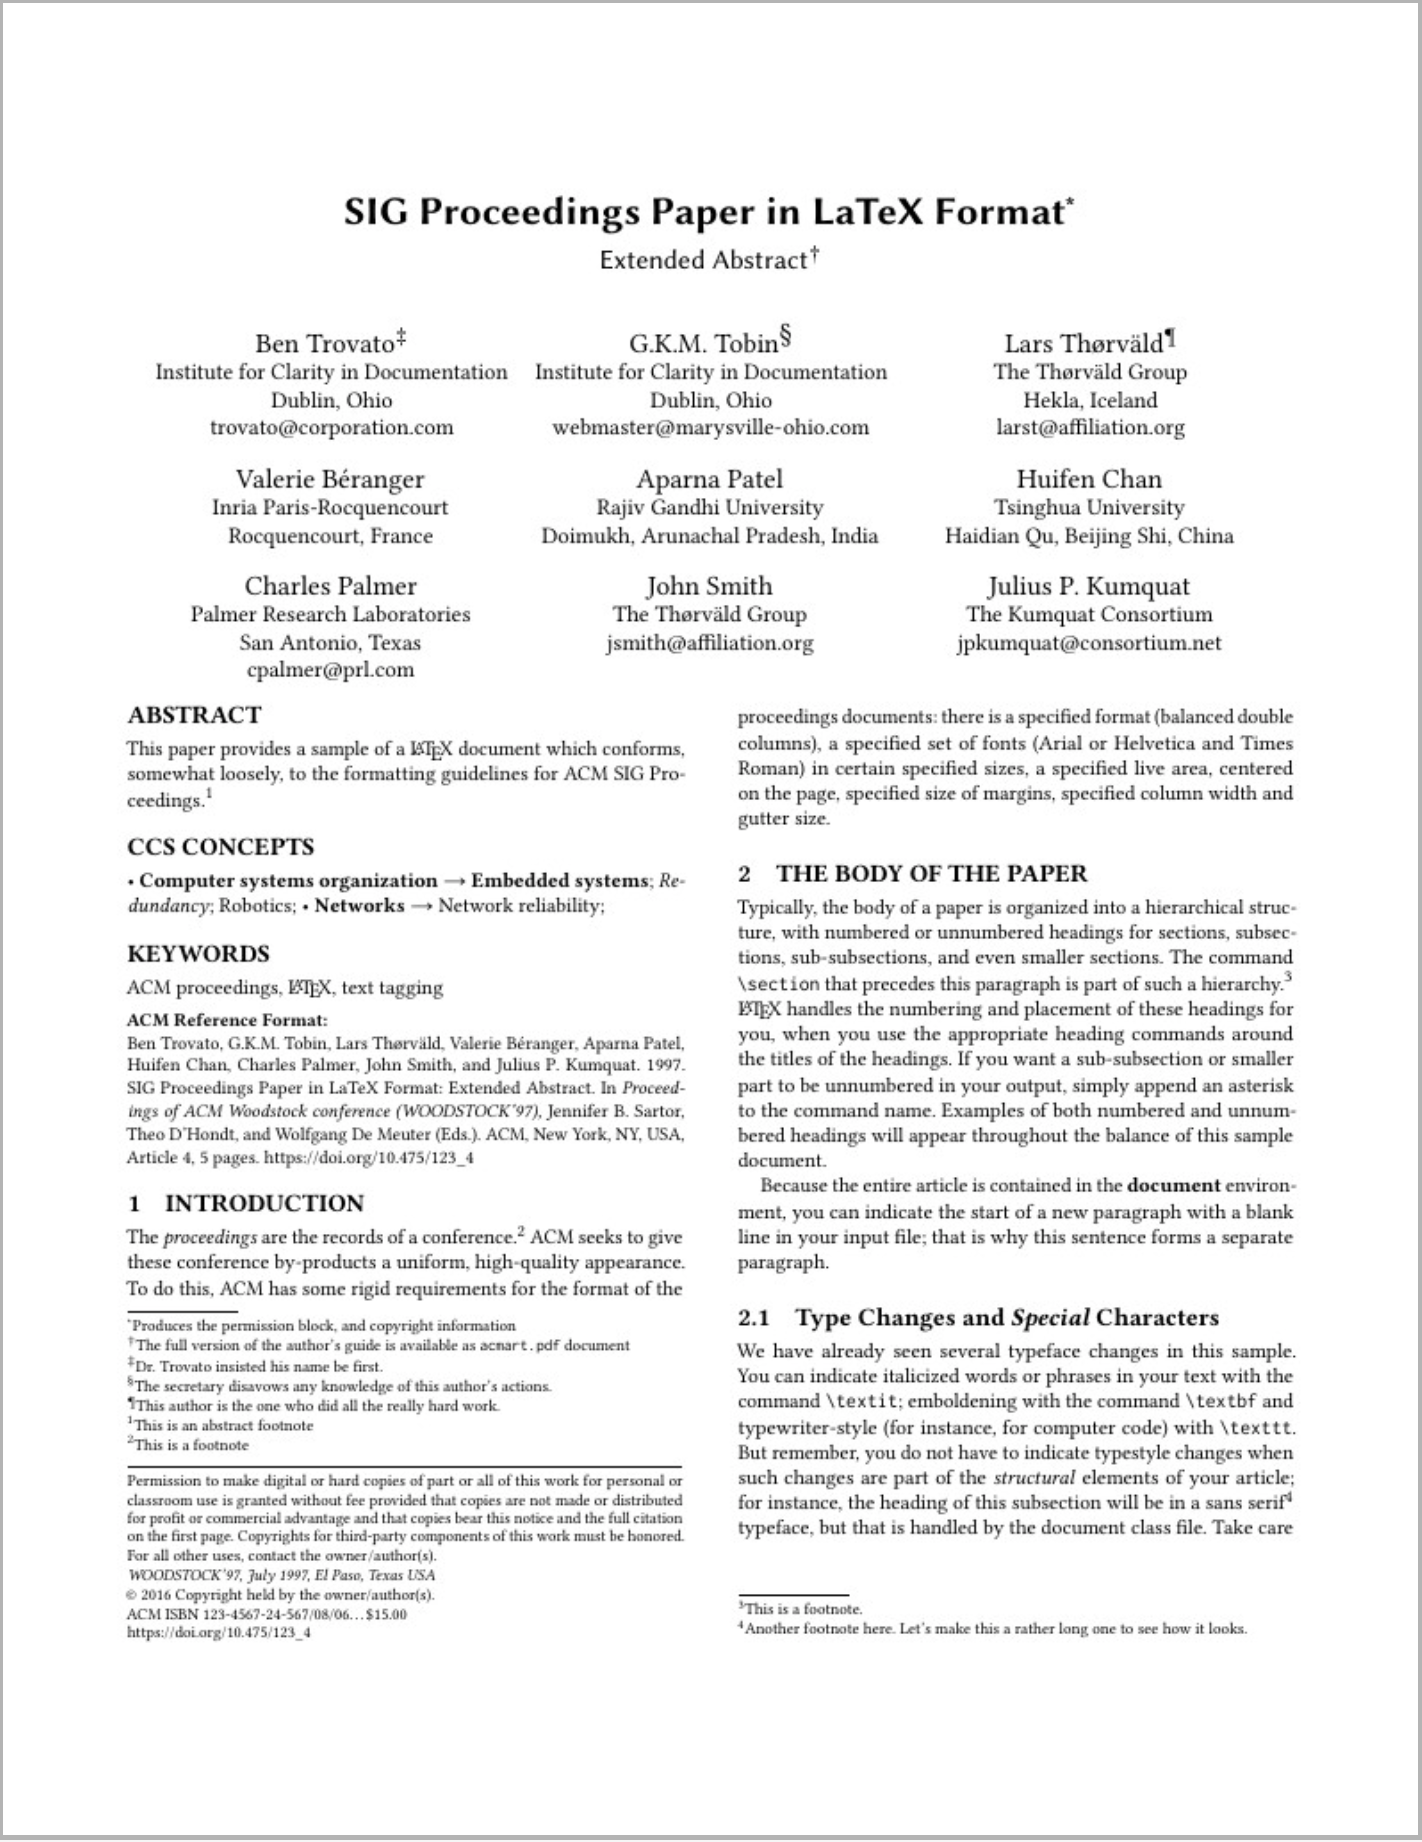
\includegraphics[width=6cm]{images/doc/acm.png}
  \hfill
  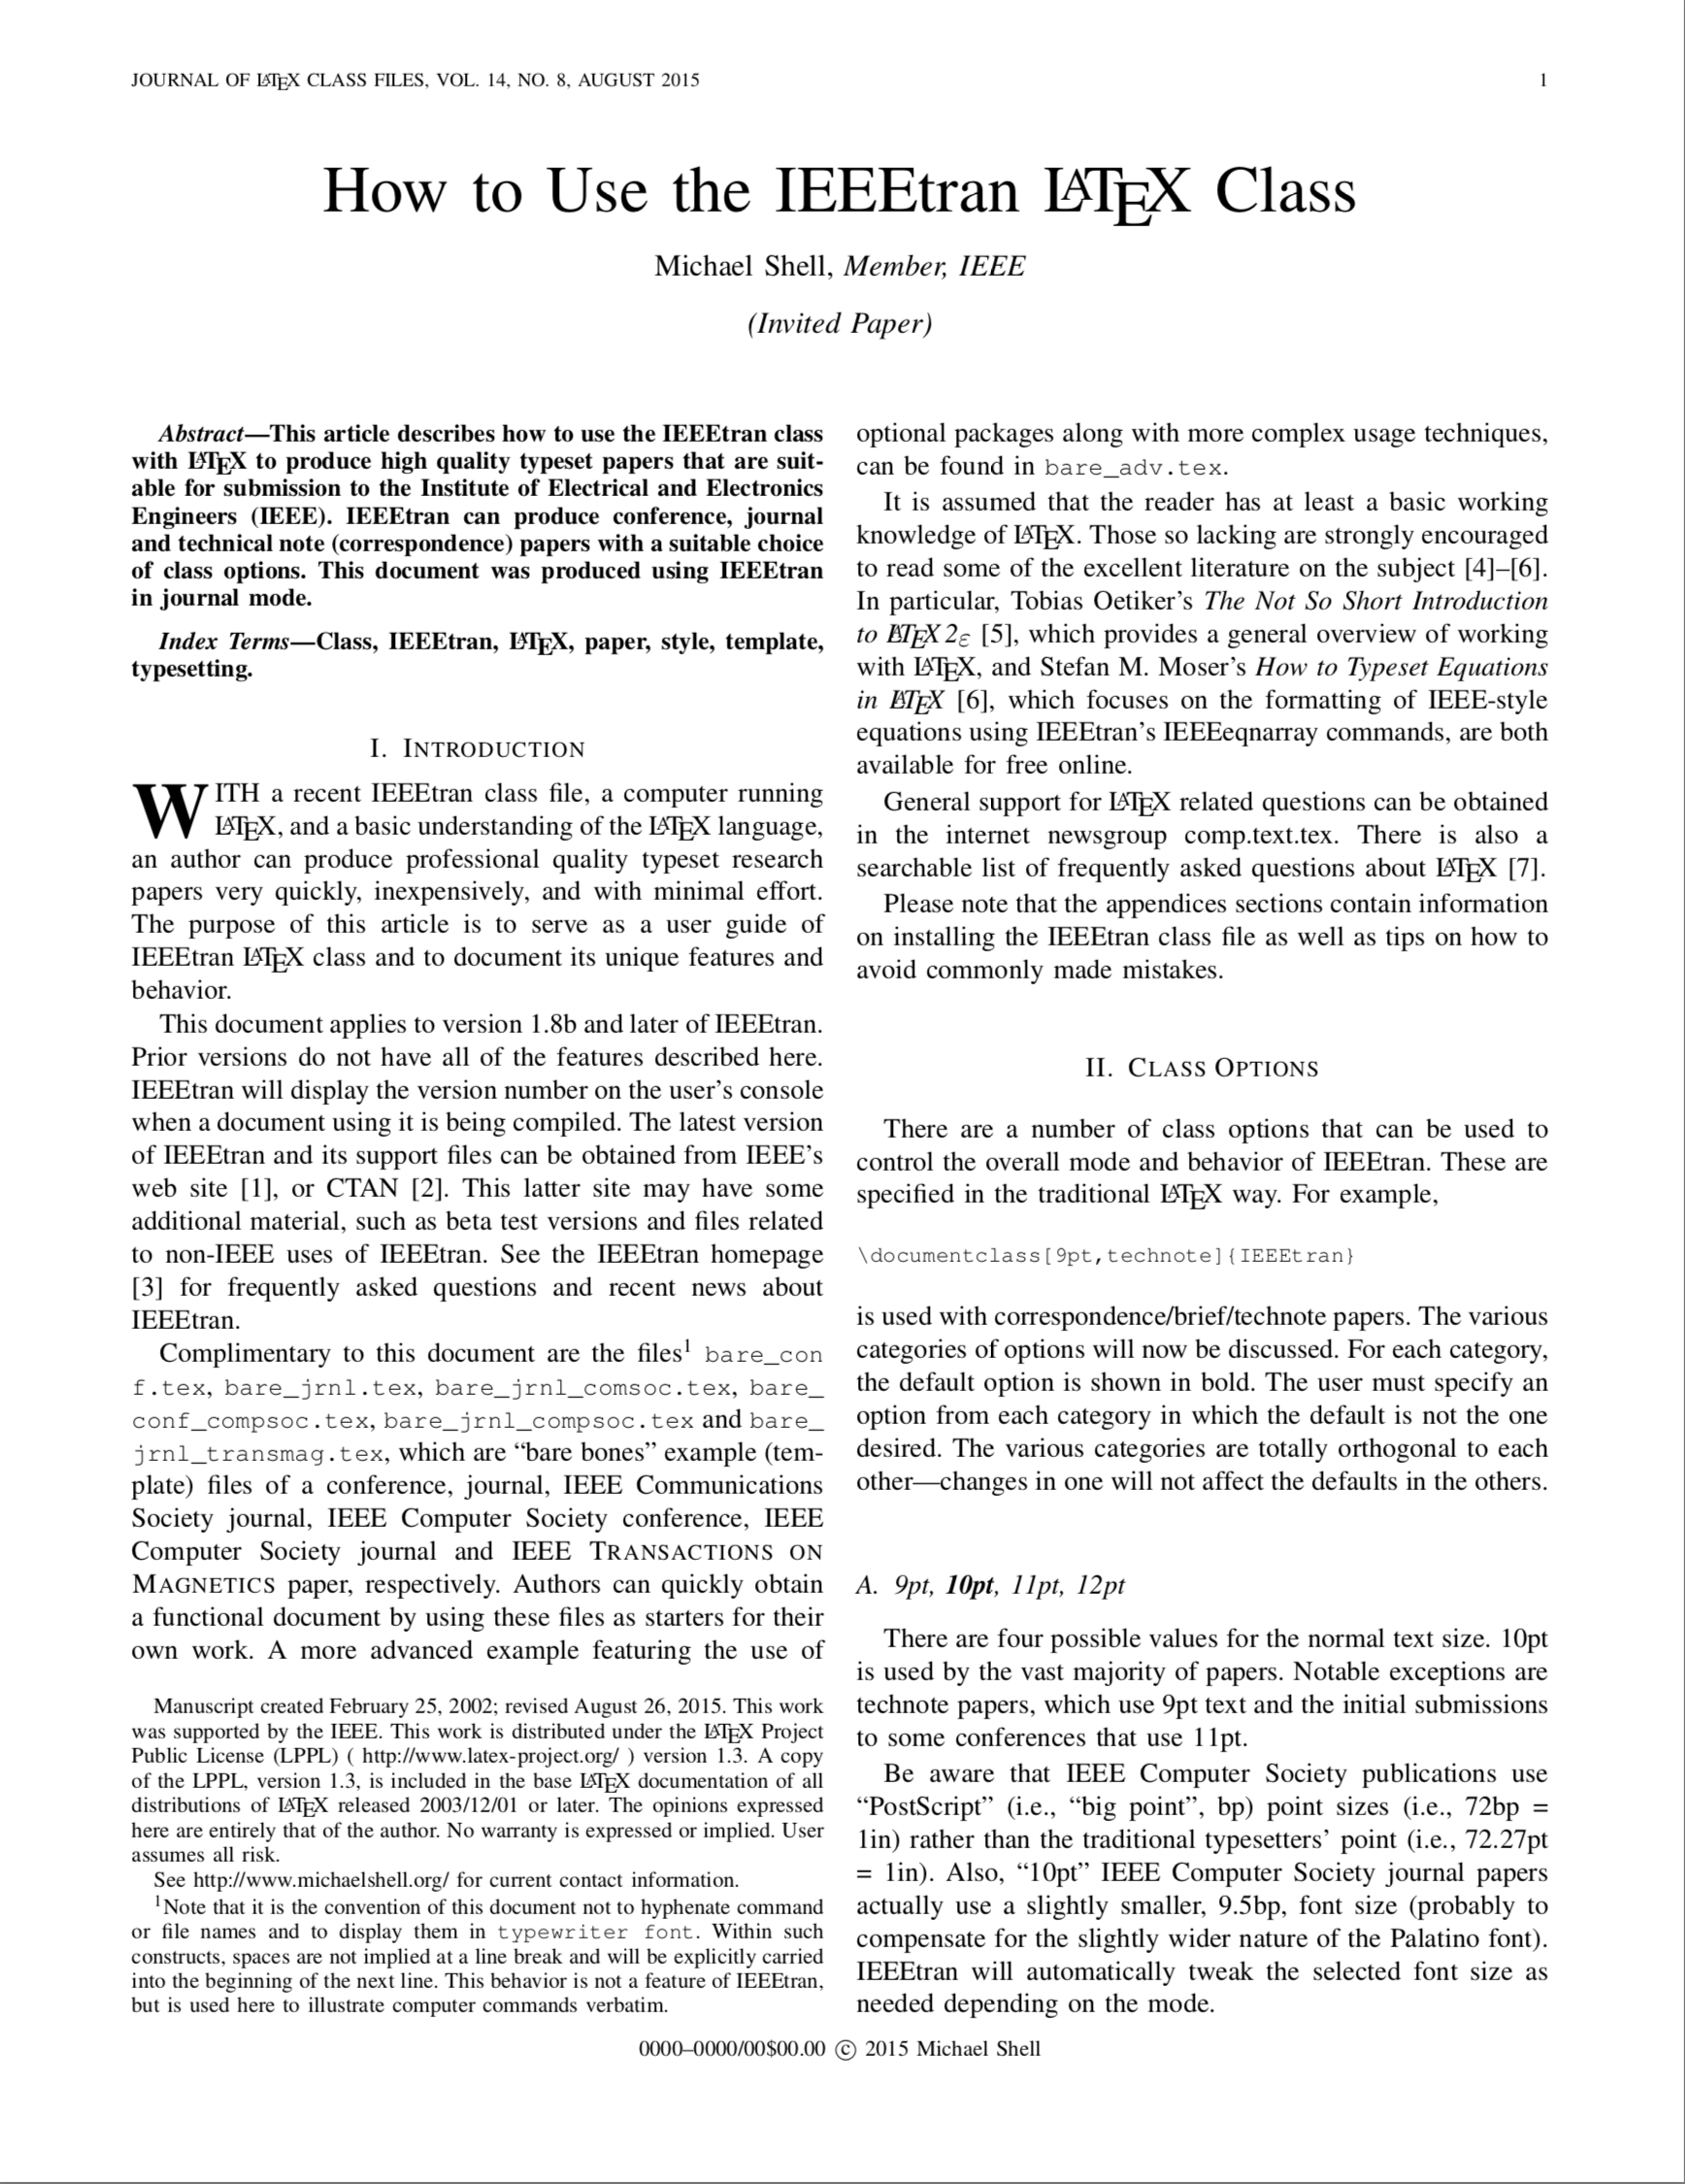
\includegraphics[width=6cm]{images/doc/ieee.png}
\caption{The look of the ACM and IEEE format templates}
\end{figure}

\begin{itemize}

\item
  \url{http://www.acm.org/publications/proceedings-template}
\item
  \url{https://www.ieee.org/conferences_events/conferences/publishing/templates.html}
\end{itemize}

\subsection{Generating and Managing Images}\label{generating-images}

To produce high quality images the programs PowerPoint and omnigraffle
on OSX are recommended. When using powerpoint please keep the image
ratio to 4x3 as they produce nice size graphics which you also can use
in your presentations. When using other rations they may not fit in
presentations and thus you may increase unnecessarily your work. We do
not recommend vizio as it is not universally available and produces
images that in case you have to present them in a slide presentation
does not easily reformat if you do not use 4x3 aspect ratio.

Naturally, graphics should be provided in SVG or PDF format so they can
scale well when we look at the final PDF. Including PNG, gif, or jpeg
files often do not result in the necessary resolution or the files
become real big. For this reason we for example can also not recommend
tools such as tablaeu as they do not provide proper exports to high
quality publication formats. For interactive display such tool may be
good, but for publications it produces inferior formatted images.

We recommend that all images be stored into a folder called images in
the same directory where your \LaTeX main document resides.


\subsection{Slides}\label{slides}
\index{Latex!slides}

Slides are best produced with the seminar package:

\begin{verbatim}
\documentclass{seminar}

\begin{slide}

    Hello World on slide 1

\end{slide}

The text between slides is ignored

\begin{slide}

    Hello World on slide 2

\end{slide}
\end{verbatim}

However, in case you need to have a slide presentation we recommend you
use ppt. Just paste and copy content from your PDF or your LaTeX source
file into the ppt.


\subsection{Useful Online Information about \LaTeX }
\index{Latex!other documentation}

\begin{description}


\item[Latex Sheet:]    \url{https://wch.github.io/latexsheet/latexsheet.pdf}

\item[Latex Short:]    \url{http://tug.ctan.org/info/lshort/english/lshort.pdf}

\item[Wikibook:]       \url{https://en.wikibooks.org/wiki/LaTeX}
\item[Wikibook (PDF)]: \url{https://upload.wikimedia.org/wikipedia/commons/2/2d/LaTeX.pdf}

\item [Links to books:] \url{https://latexforhumans.wordpress.com/2008/10/11/the-best-guides-to-latex/}
\item [Links to books:] \url{https://www.latex-project.org/help/books/}
\item [LaTeX2e:]
  The
  \href{http://texdoc.net/texmf-dist/doc/latex/latex2e-help-texinfo/latex2e.pdf}{LaTeX
  Reference Manual} provides a good introduction to Latex.

\end{description}


\begin{itemize}

\item
  LaTeX Users and Reference Guide, by Leslie Lamport
  \url{https://www.amazon.com/LaTeX-Document-Preparation-System-2nd/dp/0201529831/ref=sr_1_2?s=books\&ie=UTF8\&qid=1507114870\&sr=1-2\&keywords=lamport}
\item
  LaTeX an Introduction, by Helmut Kopka
  \url{https://www.amazon.com/Guide-LaTeX-4th-Helmut-Kopka/dp/0321173856/ref=pd_lpo_sbs_14_t_0?_encoding=UTF8\&psc=1\&refRID=2BB4APDFEX34A4JM65ZB}
\item
  The LaTeX Companion, by Frank Mittelbach
  \url{https://www.amazon.com/LaTeX-Companion-Techniques-Computer-Typesetting/dp/0201362996}
\end{itemize}



\subsection{LaTeX vs. X}\label{latex-vs.-x}

We will refrain from providing a detailed analysis on why we use LaTeX
in many cases versus other technologies. In general, we find that LaTeX:

\begin{itemize}
\tightlist
\item
  is incredibly stable
\item
  produces high-quality output
\item
  is platform independent
\item
  has lots of templates
\item
  has been around for many years so it works well
\item
  removes you from the pain of figure placements
\item
  focusses you on content rather tan the appearance of the paper
\item
  integrates well with code repositories such as git to write
  collaborative papers.
\item
  has superior bibliography integration
\item
  has a rich set of tools that make using LaTeX easier
\item
  authors do not play with layouts much so papers in a format are
  uniform
\end{itemize}

In case you need a graphical view to edit LaTeX or LateX exportable
files you also find AucTeX and Lyx.

\subsubsection{Word}\label{word}

Word is arguably available to many, but if you work on Linux you may be
out of luck. Also Word often focusses not on structure of the text but
on its appearance. Many students abuse Word and the documents in Word
become a pain to edit with multiple users. Recently Microsoft has
offered online services to collaborate on writing documents in groups
which work well. Integration with bibliography managers such as endnote
or Mendeley is possible.

However, we ran into issues whenever we use word:

\begin{itemize}
\tightlist
\item
  Word tends sometimes to crash for unknown reasons and we lost a lot of
  work
\item
  Word has some issues with the bibliography managers and tends to crash
  sometimes for unknown reasons.
\item
  Word is slow with integration to large bibliographies.
\item
  Figure placement in Word in some formats is a disaster and you will
  spend many hours to correct things just to find out that if you make
  small changes you have to spend additional many hours to get used to
  the new placement. We have not yet experienced a word version where we
  have not lost images. Maybe that has changed, so let us know
\end{itemize}

However, we highly recommend the collaborative editing features of Word
that work on a paragraph and not letter level. Thus saving is essential
so you do not block other people from editing the paragraph.

\subsubsection{Google Docs}\label{google-docs}

Unfortunately, many useful features got lost in the new google docs.
However, it is great to collaborate quickly online, share thoughts and
even write your latex documents together if you like (just copy your
work in a file offline and use latex to compile it ;-) )

The biggest issue we have with Google Docs is that it does not allow the
support of 2 column formats, that the bibliography integration is
non-existent and that paste and copy from web pages and images
encourages unintended plagiarism when collecting information without
annotations (LaTeX and Word are prone to this too, but we found from
experience that it tends to happen more with Google docs users.

\subsubsection{A Place for Each}\label{a-place-for-each}

When looking at the tools we find a place for each:

\begin{description}
\item[Google docs:]
Short meeting notes, small documents, quick online collaborations to
develop documents collaboratively at the same time.
\item[Word:]
Available to many, supports 2 column format, supports paragraph based
collaborative editing, Integrates with bibliography managers.
\item[LaTeX:]
Reduces failures, great offline editing, superior bibliography
management, superior image placement, runs everywhere. Great
collaborative editing with sharelatex, allows easy generation of
proceedings written by hundreds of people with shared index.
\item[The best choice for your class:]
LaTeX
\end{description}

\section{Editing}\label{editing}

\subsection{Emacs}\label{emacs}

The text editor emacs provides a great basis for editing TeX and LaTeX
documents. Both modes are supported. In addition there exists a color
highlight module enabling the color display of LaTeX and TeX commands.
On OSX aquaemacs and carbon emacs have build in support for LaTeX. Spell
checking is done with flyspell in emacs.

\subsubsection{Aquamacs}

Aquamacs is an editor based on GNU Emacs that runs on OSX and
integrates with the OSX desktop. This is for many the preferred editor
on OSX for \LaTeX.

\url{http://aquamacs.org}

\begin{figure}[!h]
  \centering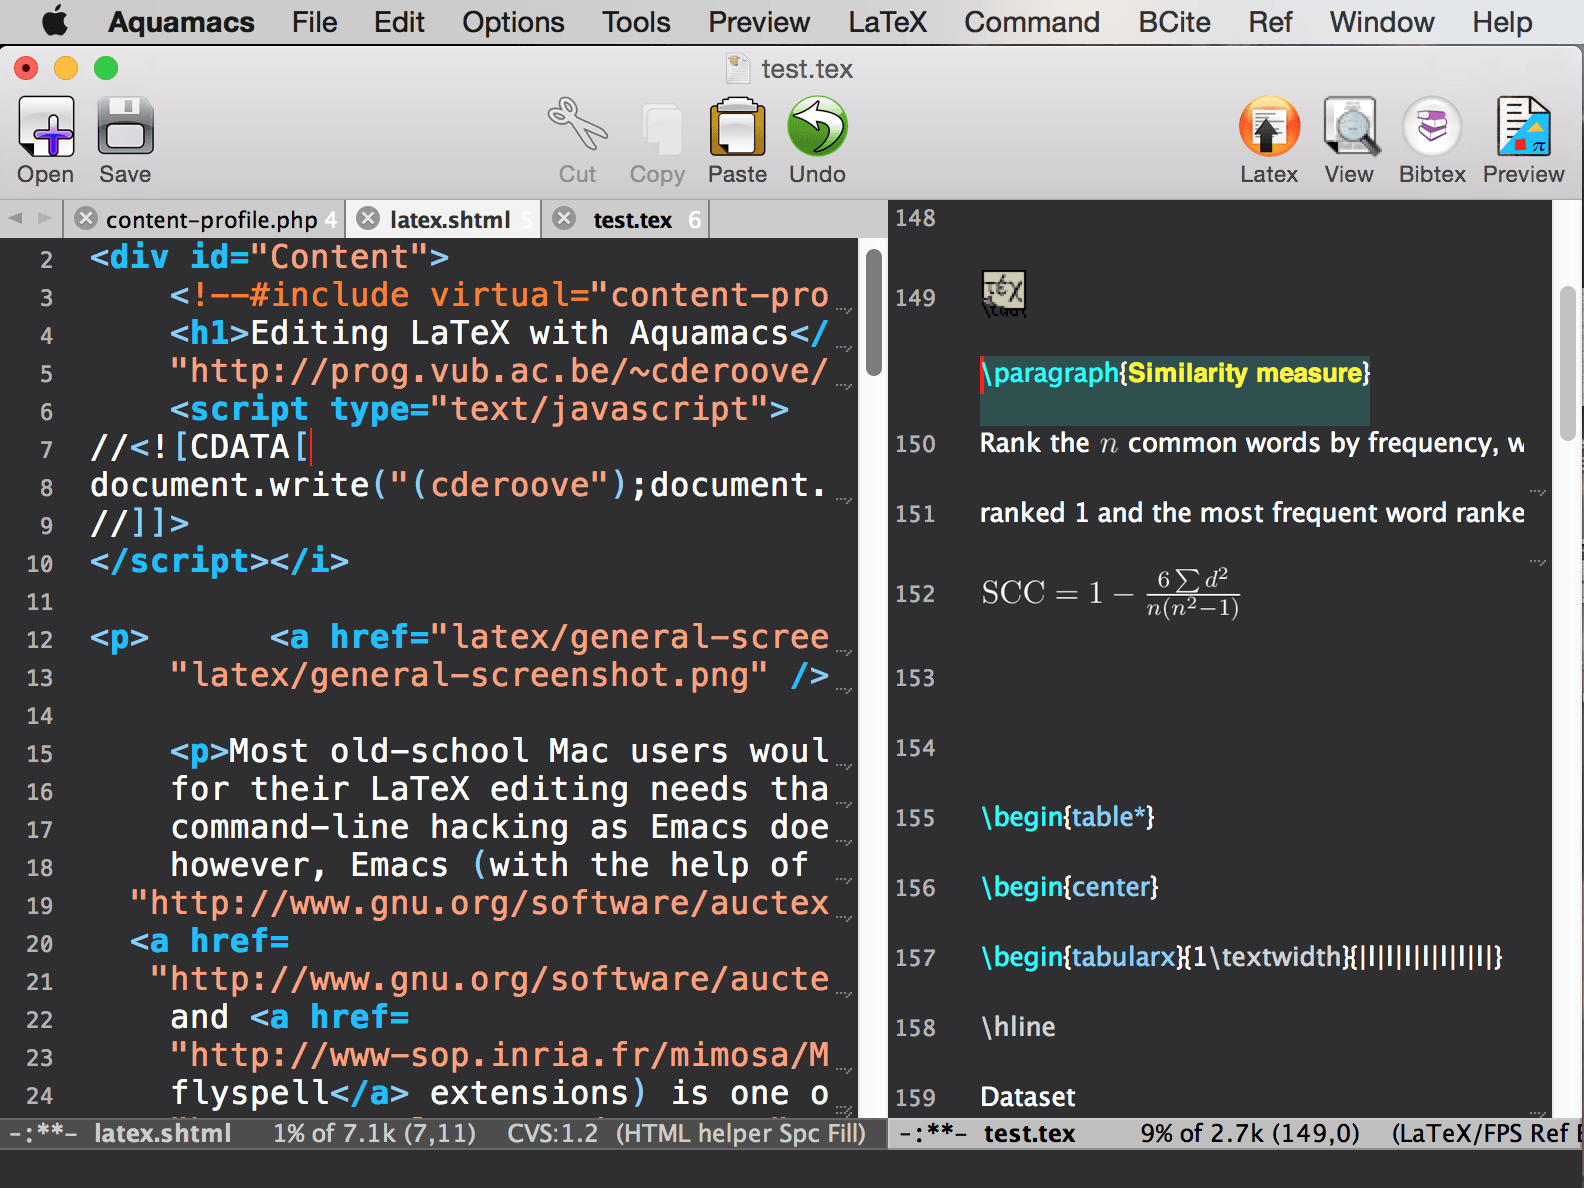
\includegraphics[width=8cm]{images/aquamacs.png}
  \caption{Aquamacs}
  \label{F:aquamacs}
\end{figure}


\subsection{Vi/Vim}\label{vivim}

Another popular editor is vi or vim. It is less feature rich but many
programmers ar using it. As it can edit ASCII text you can edit LaTeX.
With the LaTeX add-ons to vim, vim becomes similar powerful while
offering help and syntax highlighting for LaTeX as emacs does. (The
authors still prefer emacs)

\subsection{TeXshop}\label{texshop}

Other editors such as TeXshop are available which provide a more
integrated experience. However, we find them at times to stringent and
prefer editors such as emacs.

\subsection{LyX}\label{lyx}

We have made very good experiences with Lyx. You must assure that the
team you work with uses it consistently and that you all use the same
version.

\begin{figure}[!h]
  \centering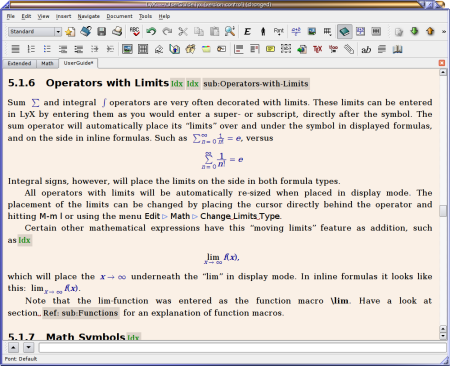
\includegraphics[width=8cm]{images/lyx.png}
  \caption{Lyx}
  \label{F:lyx}
\end{figure}

Using the ACM templates is documented here:

\begin{itemize}
\tightlist
\item
  \url{https://wiki.lyx.org/Examples/AcmSiggraph}
\end{itemize}

On OSX it is important that you have a new version of LaTeX and Lyx
installed. As it takes up quite some space, you ma want to delete older
versions. The new version of LyX comes with the acmsigplan template
included. However on OSX and other platforms the .cls file is not
included by default. However the above link clearly documents how to fix
this.

\subsection{WYSIWYG locally}\label{wysiwyg-locally}

We have found that editors such as Lyx and Auctex provide very good
WYSIWYG alike features. However, we found an even easier way while using
skim, a pdf previewer, in conjunction with emacs and latexmk. This can
be achieved while using the following command assuming your latex file
is called `report.tex`:

\begin{verbatim}
latexmk -pvc -view=pdf report
\end{verbatim}

This command will update your pdf previewer (make sure to use skim)
whenever you edit the file report.tex and save it. It will maintain via
skim the current position, thus you have a real great way of editing in
one window, while seeing the results in the other.

Skim can be found at: \url{http://skim-app.sourceforge.net/}

\subsection{Markdown and \LaTeX}
\index{Latex!markdown}

It may come as a surprise to many that one can actually write simple
LaTeX documents also in markdown Syntax or mix section written in
markdown while others are written in LaTeX. To do so all you ahve to
do is place the markdown text in a separate file. Let us call the file 
content.rst which has the following lines included in it:

\begin{verbatim}
# Section

* item a
* item b
\end{verbatim}

Obviously, we would have to convert this to LaTeX. Luckily there is a
very useful program called {\em pandoc} that does this for you. YOu
could make the translation in the shell, but you could also make the
translation locally on your computer while allowing \LaTeX to start up
external programs. This is achieved with the {\em write18} command and
allowing LaTeX explicitly to call external programs. Please inspect
the following latex file that includes a template on how to do
this. We assume the file is called markdown.tex for our example.

\begin{verbatim}
\documentclass{article}

\include{graphicx}
\newcommand{\tightlist}{}

\begin{document}
\immediate\write18{pandoc content.md -o content.tex}

\MDNAME
%%%%%%%%%%%%%%%%%%%%%%%%%%%%%%%%%%%%%%%%%%%%%%%%%%%%%%%%%%%%%%%%%%%%%%%%%%%%%%%
% DO NOT MODIFY THIS FILE
%%%%%%%%%%%%%%%%%%%%%%%%%%%%%%%%%%%%%%%%%%%%%%%%%%%%%%%%%%%%%%%%%%%%%%%%%%%%%%%




\end{document}
\end{verbatim}

Now to generate the PDF we simply have to call the following command
that include the {\em -shell-escape} flag to allow the execution of
write18 embedded commands:

\begin{verbatim}
pdflatex -shell-escape markdown-test
\end{verbatim}

The output will be {\em markdown.pdf} with the content from the
markdown file translated. Doing this naturally allows you to write
large portions in markdown and automatically include them in your
LaTeX document. Hence, you can use editors such as Macdown to initially
work in semi WYSIWYG mode and do fairly straight forward
edition. Naturally the same can be done in RST. Naturally the most
elementary features are supported. For more sophisticated features,
please use LaTeX directly.

\subsection{pyCharm}

TODO: comment on how we can use pycharm for editing and what the
limitations are.

\subsection{MSWord}

it is possible to use Word.

be careful with 

\section{The LaTeX Cycle}\label{the-latex-cycle}
\index{Latex!cycle}

To create a PDF file from latex yo need to generate it following a
simple development and improvement cycle.

First, Create/edit ASCII source file with \texttt{file.tex} file:

\begin{verbatim}
emacs file.tex
\end{verbatim}

Create/edit bibliography file:

\begin{verbatim}
jabref refs.bib
\end{verbatim}

Create the PDF:

\begin{verbatim}
pdflatex file
bibtex file
pdflatex file
pdflatex file
\end{verbatim}

View the PDF:

\begin{verbatim}
open file
\end{verbatim}

It not only showcases you an example file in ACM 2 column format, but
also integrates with a bibliography. Furthermore, it provides a sample
Makefile that you can use to generate view and recompile, or even
autogenerate. A compilation would look like:

\begin{verbatim}
make
make view
\end{verbatim}

If however you want to do things on change in the tex file you can do
this automatically simply with:

\begin{verbatim}
make watch
\end{verbatim}

for make watch its best to use skim as pdf previewer


\section{Tips}\label{tips}

Including figures over two columns:

\begin{itemize}
\item
  \url{http://tex.stackexchange.com/questions/30985/displaying-a-wide-figure-in-a-two-column-document}
\item
  positioning figures with textwidth and columnwidth
  \url{https://www.sharelatex.com/learn/Positioning_images_and_tables}
\item
  An organization as the author. Assume the author is National Institute
  of Health and want to have the author show up, please do:

\begin{verbatim}
key= {National Institute of Health},
author= {{National Institute of Health}},
\end{verbatim}

  Please note the \{\{ \}\}
\item
  words containing `fi' or `ffi' showing blank places like below after
  recompiling it: find as nd efficiency as e ciency

  You copied from word or PDF ff which is actually not an ff, but a
  condensed character, change it to ff and ffi, you may find other such
  examples such as any non ASCII character. A degree is for example
  another common issue in data science.
\item
  do not use \textbar{} \& and other latex characters in bibtex
  references, instead use , and the word and
\item
  If you need to use \_ it is \_ but if you use urls leave them as is
\item
  We do recommend that you use sharelatex and jabref for writing papers.
  This is the easiest solution and beats in many cases MSWord as you can
  focus on writing and not on formatting.
\end{itemize}


\chapter{Managing Bibliographies}

\begin{fileremark}\url{https://github.com/cloudmesh/classes/blob/master/docs/source/lesson/doc/bibtex.rst}\end{fileremark}

\subsection{Integrating Bibliographies}\label{bibliographies}

LaTeX integrates very well with bibtex. There are several pre-formated
styles available. It includes also styles for ACM and IEEE
bibliographies. For the ACM style we recommend that you replace
abbrv.bst with abbrvurl.bst, add hyperref to your usepackages so you can
also display URLs in your citations:

\begin{verbatim}
\bibliographystyle{IEEEtran}
\bibliography{references.bib}
\end{verbatim}

Then you have to run latex and bibtex in the following order:

\begin{verbatim}
latex  file
bibtex file
latex  file
latex  file
\end{verbatim}

or simply call make from our makefile.

The reason for the multiple execution of the latex program is to update
all cross-references correctly. In case you are not interested in
updating the library every time in the writing progress just postpone it
till the end. Missing citations are viewed as {[}?{]}.

Two programs stand out when managing bibliographies: emacs and jabref:

\begin{itemize}
\tightlist
\item
  \url{http://www.jabref.org/}
\end{itemize}

Other programs such as Mendeley, Zotero, and even endnote integrate with
bibtex. However their support is limited, so we recommend that you just
use jabref. Furthermore its free and runs on all platforms.

\subsubsection{jabref}\label{jabref}

Jabref is a very simple to use bibliography manager for LaTeX and other
systems. It can create a multitude of bibliography file formats and
allows upload in other online bibliography managers.

\begin{itemize}
\tightlist
\item
  Installation: Go to \url{http://www.jabref.org/} and click download
\item
  Video: \url{https://youtu.be/cMtYOHCHZ3k}
\item
  Video with cc: \url{https://www.youtube.com/watch?v=QVbifcLgMic}
\end{itemize}

\subsubsection{jabref and MSWord}\label{jabref-and-msword}

According to others it is possible to integrate jabref references
directly into MSWord. This has been conducted so far however only on a
Windows computer.

We have not tried this ourselves, but give it as a potential option.

Here are the steps the need to be done:

\begin{enumerate}
\def\labelenumi{\arabic{enumi}.}
\tightlist
\item
  Create the Jabref bibliography just like in presented in the Jabref
  video
\item
  After finishing adding your sources in Jabref, click
  File -\textgreater{} export
\item
  Name your bibliography and choose MS Office 2007(*.xml) as the file
  format. Remember the location of where you saved your file.
\item
  Open up your word document. If you are using the ACM template, go
  ahead and remove the template references listed under
  Section 7. References
\item
  In the MS Word ribbon choose `References'
\item
  Choose `Manage Sources'
\item
  Click `Browse' and locate/select your Jabref xml file
\item
  You should now see your references appear in the left side window.
  Select the references you want to add to your document and click the
  `copy' button to move them from the left side window to the right
  window.
\item
  Click the `Close' button
\item
  In the MS Word Ribbon, select `Bibliography' under the References tab
\item
  Click `Insert Bibliography' and your references should appear in the
  document
\item
  Ensure references are of Style: IEEE. Styles are located in the
  References tab under `Manage Sources'
\end{enumerate}

As you can see there is significant effort involve, so we do recommend
you use LaTeX as you can focus there on content rather than dealing with
complex layout decisions. This is especially true, if your papers have
figures or tables, or you need to add references.


\section{Entry types}

In this section we will explain how to find and properly generate
bibliographic entries. We are using bibtex for this as it is easy to use
and generates reasonable entries that can be included in papers. What we
like to achieve in this section is not to just show you a final entry,
but to document the process on how that entry was derived. This will
allow you to replicate or learn from the process to apply to your own
entries.

We will address a number of important entry types which includes:

\begin{itemize}
\tightlist
\item
  wikipedia entries
\item
  github entries
\item
  books
\item
  articles in a scientific journal
\item
  articles in a conference
\item
  articles in magazines (non scientific)
\item
  blogs
\end{itemize}

\subsection{Source code References}\label{source-code-references}

We will learn how to cite a source code from a publicly hosted
repository. Such repositories are frequently used and include, for
example github, bitbucket, sourcefore, or your Universities code
repository as long as it is publicly reachable. As changes can occur on
these repositories, it is important that the date ov access is listed in
the entry or even the release version of the source code.

Let us without bias chose a random source dode entry that has been
contributed by a student as follows:

\begin{verbatim}
@Misc{gonzalez_2015,
  Title =  {Buildstep},
  Author =     {Gonzalez, Jose and Lindsay,Jeff},
  HowPublished = {Web Page},
  Month =  {Jul},
  Note =   {Accessed: 2017-1-24},
  Year =   2015,
  Key =        {www-buildstep},
  Url =        {https://github.com/progrium/buildstep}
}
\end{verbatim}

Is this entry correct? Let us analyse.

\subsubsection{Entry type Misc}\label{entry-type-misc}

First, it seems appropriate to use a \emph{@misc} entry. We correctly
identify this is a misc entry as it is online available. More recent
version of bibtex include also the type \emph{@online} for it. However,
in order to maintain compatibility to older formats we chose simply Misc
here and if we really would need to we could replace it easily

\subsubsection{Label}\label{label}

Typically the Label should contain 3 letters from an author name, short
year and the short name of the publication to provide maximum
information regarding the publication. Underscores need to be replaced
by dashes or removed. However as this is a github repository it is
better to integrate this into the label. Hence, we simply use the
github-projectname (in our case github-buildstep, out of convention we
only use lower case letters.

\subsubsection{Author}\label{author}

Unless the last name contains spaces, it should be first name followed
by the last name with multiple authors separated with ``and''.

\subsubsection{Key}\label{key}

In this case the key field can be removed as the entry has an author
field entry. If there was no author field, we could use key to specify
the alphabetical ordering based on the specified key. Note that a key is
not the label. In fact in our original entry the key field was wrongly
used and the student did not understand that the key is used for
sorting.

\subsubsection{Howpublished}\label{howpublished}

Since the source is a github project repository, the howpublished field
shall hold the value \{Code Repository\} rather than a web page. If the
url specified was a normal webpage, the \{Web Page\} entry would be
valid.

\subsubsection{Month}\label{month}

The lowercase month is, used for international notation since months are
not capitalized in some other languages.

\subsubsection{Owner}\label{owner}

In class we introduced the convention to put the student HID in it. If
multiple students contributed, add them with space separation.

\subsubsection{Accessed}\label{accessed}

As we do not yet typically an accessed field, we simply include it in
the note field. This is absolutely essential as code can change and when
we read the code we looked at a particular snapshot in time. In addition
it is often necessary to record the actual version of the code.
Typically this can also be done with the month and year field while
relying on a release date

\subsubsection{Final Entry}\label{final-entry}

Filling out as many fields as possible with information for this entry
we get:

\begin{verbatim}
@Misc{github-buildstep,
  Title =  {Buildstep},
  Author =     {Jose Gonzalez and Jeff Lindsay},
  HowPublished = {Code Repository},
  Year =   {2015},
  Month =  jul,
  Note =   {Accessed: 2017-1-24},
  Url =    {https://github.com/progrium/buildstep},
  Owner =  {S17-IO-3025},
}
\end{verbatim}

We are using the release date in the year and month field as this
project uses this for organizing releases. However, other project may
have release versions so you would have in addition to using the data
also to include the version in the note field such as:

\begin{verbatim}
Note =     {Version: 1.2.3, Accessed: 2017-1-24},
\end{verbatim}

\begin{description}
\item[All those that helped should add your HID to this entry with]
a space separated from each other
\end{description}

\subsection{Researching proper bibtex
entries}\label{researching-proper-bibtex-entries}

\subsubsection{Article in a journal}\label{article-in-a-journal}

Many online bibtex entries are wrong or incomplete. Often you may find
via google a bibtex entry that may need some more research. Lets assume
your first google query returns a publication and you cite it such as
this:

\begin{verbatim}
@Unpublished{unpublished-google-sawzall,
    Title = {{Interpreting the Data: Parallel Analysis with Sawzall}},
    Author = {{Rob Pike, Sean Dorward, Robert Griesemer, Sean Quinlan}},
    Note = {accessed 2017-01-28},
    Month = {October},
    Year = {2005},
    Owner = {for the purpose of this discussion removed},
    Timestamp = {2017.01.31}
}
\end{verbatim}

Could we improve this entry to achieve your best? We observe:

\begin{enumerate}
\def\labelenumi{\arabic{enumi}.}
\tightlist
\item
  The author field has a wrong entry as the , is to be replaced by an
  and.
\item
  The author feild has authors and thus must not have a \{\{ \}\}
\item
  The url is missing, as the simple google search actually finds a PDF
  document.
\end{enumerate}

Let us investigate a bit more while searching for the title. We find

\begin{enumerate}
\def\labelenumi{\Alph{enumi})}
\tightlist
\item
  \url{https://www.google.com/url?sa=t\&rct=j\&q}=\&esrc=s\&source=web\&cd=1\&ved=0ahUKEwj\_ytSA-PDRAhUH8IMKHaomC-oQFggaMAA\&url=https\%3A\%2F\%2Fresearch.google.com\%2Farchive\%2Fsawzall-sciprog.pdf\&usg=AFQjCNHSSfKBwbxVAVPQ0td4rTjitKucpA\&sig2=vbiVzi36B3gGFjIzlUKBDA\&bvm=bv.146073913,d.amc
\item
  \url{https://research.google.com/pubs/pub61.html}
\item
  \url{http://dl.acm.org/citation.cfm?id=1239658}
\end{enumerate}

Let us look at A)

As you can see from the url this is actually some redirection to a google
web page which probably is replaced by B as its from google research. So
let us look at B)

Now when you look at the link we find the url
\url{https://research.google.com/archive/sawzall-sciprog.pdf} which
redirects you to the PDF paper.

When we go to B) we find surprisingly a bibtex entry as follows:

\begin{verbatim}
@article{61,
  title = {Interpreting the Data: Parallel Analysis with Sawzall},
  author = {Rob Pike and Sean Dorward and Robert Griesemer and Sean Quinlan},
  year = 2005,
  URL = {https://research.google.com/archive/sawzall.html},
  journal = {Scientific Programming Journal},
  pages = {277--298},
  volume = {13}
}
\end{verbatim}

Now we could say lets be satisfied, but C) seems to be even more
interesting as its from a major publisher. So lats just make sure we
look at C)

If you go to C, you find under the colored box entitled Tools and
Resources a link called \textbf{bibtex}. Thus it seems a good idea to
click on it. This will give you:

\begin{verbatim}
@article{Pike:2005:IDP:1239655.1239658,
    author = {Pike, Rob and Dorward, Sean and Griesemer, Robert and Quinlan, Sean},
    title = {Interpreting the Data: Parallel Analysis with Sawzall},
    journal = {Sci. Program.},
    issue_date = {October 2005},
    volume = {13},
    number = {4},
    month = oct,
    year = {2005},
    issn = {1058-9244},
    pages = {277--298},
    numpages = {22},
    url = {http://dx.doi.org/10.1155/2005/962135},
    doi = {10.1155/2005/962135},
    acmid = {1239658},
    publisher = {IOS Press},
    address = {Amsterdam, The Netherlands, The Netherlands},
}
\end{verbatim}

Now we seem to be at a position to combine our search result as neither
entry is sufficient. As the doi number properly specifies a paper (look
up what a doi is) we can replace the url with one that we find online,
such as the one we found in A) Next we see that all field sin B are
already covered in C, so we take C) and add the url. Now as the label is
great and uniform for ACM, but for us a bit less convenient as its
difficult to remember, we just change it while for example using
authors, title, and year information. lets also make sure to do mostly
lowercase in the label just as a convention. Thus our entry looks like:

\begin{verbatim}
@article{pike05swazall,
    author = {Pike, Rob and Dorward, Sean and Griesemer, Robert and Quinlan, Sean},
    title = {Interpreting the Data: Parallel Analysis with Sawzall},
    journal = {Sci. Program.},
    issue_date = {October 2005},
    volume = {13},
    number = {4},
    month = oct,
    year = {2005},
    issn = {1058-9244},
    pages = {277--298},
    numpages = {22},
    url = {https://research.google.com/archive/sawzall-sciprog.pdf},
    doi = {10.1155/2005/962135},
    acmid = {1239658},
    publisher = {IOS Press},
    address = {Amsterdam, The Netherlands, The Netherlands},
}
\end{verbatim}

As you can see properly specifying a reference takes multiple google
queries and merging of the results you find from various returns. As
you still have time to correct things I advise that you check your
references and correct them. If the original reference would have been
graded it would have been graded with a ``fail'' instead of a ``pass''.

\subsection{Article in a conference
proceedings}\label{article-in-a-conference-proceedings}

Lets look at a second obvious example that needs improvement:

\begin{verbatim}
@InProceedings{wettinger-any2api,
  Title                    = {Any2API - Automated APIfication},
  Author                   = {Wettinger, Johannes and
                              Uwe Breitenb{\"u}cher
                              and Frank Leymann},
  Booktitle                = {Proceedings of the 5th International
                              Conference on Cloud Computing and
              Services Science},
  Year                     = {2015},
  Pages                    = {475­486},
  Publisher                = {SciTePress},

  ISSN                     = {2326-7550},
  Owner                    = {S17-IO-3005},
  Url                      = {https://pdfs.semanticscholar.org/1cd4/4b87be8cf68ea5c4c642d38678a7b40a86de.pdf}
}
\end{verbatim}

As you can see this entry seems to define all required fields, so we
could be tempted to stop here. But its good to double check. Lets do
some queries against ACM, . and google scholar, so we just type in the
title, and if this is in a proceedings they should return hopefully a
predefined bibtex record for us.

Lets query:

\begin{verbatim}
google: googlescholar Any2API Automated APIfication
\end{verbatim}

We get:

\begin{itemize}
\tightlist
\item
  \url{https://scholar.google.de/citations?view_op=view_citation\&hl=en\&user=j6lIXt0AAAAJ\&citation_for_view=j6lIXt0AAAAJ:8k81kl-MbHgC}
\end{itemize}

On that page we see
\href{https://scholar.google.com/scholar_lookup?title=Automated+drug+dispensing+system+reduces+medication+errors+in+an+intensive+care+setting\&author=Chapuis\&publication_year=2010\#}{Cite}

So we find a PDF at
\url{https://pdfs.semanticscholar.org/1cd4/4b87be8cf68ea5c4c642d38678a7b40a86de.pdf}

Lets click on this and the document includes a bibtex entry such as:

\begin{verbatim}
@inproceedings{Wettinger2015, 
  author= {Johannes Wettinger and Uwe Breitenb{\"u}cher and Frank
       Leymann},
  title = {Any2API - Automated APIfication},
  booktitle = {Proceedings of the 5th International Conference on Cloud
       Computing and Service Science (CLOSER)},
  year = {2015},
  pages = {475--486},
  publisher = {SciTePress}
} 
\end{verbatim}

Now lets add the URL and owner:

\begin{verbatim}
@inproceedings{Wettinger2015, 
  author= {Johannes Wettinger and Uwe Breitenb{\"u}cher and Frank
       Leymann},
  title = {Any2API - Automated APIfication},
  booktitle = {Proceedings of the 5th International Conference on Cloud
       Computing and Service Science (CLOSER)},
  year = {2015},
  pages = {475--486},
  publisher = {SciTePress},
  url ={https://pdfs.semanticscholar.org/1cd4/4b87be8cf68ea5c4c642d38678a7b40a86de.pdf},
  owner = {S17-IO-3005},
} 
\end{verbatim}

Should we be satisfied? No, even our original information we gather
provided more information. So lets continue. Lets googlesearch different
queries with ACM or IEEE and the title. When doing the IEEE in the
example we find an entry called

\href{http\%3A\%2F\%2Fdblp.uni-trier.de\%2Fpers\%2Fl\%2FLeymann\%3AFrank\&usg=AFQjCNHCu-66qxWH0zRlPLr4DA8jIo5V-g\&sig2=1vYdnGOEiMcLBEMpbeBA7g}{dlp:
Frank Leyman}

Lets look at it and we find two entries:

\begin{verbatim}
@inproceedings{DBLP:conf/closer/WettingerBL15,
  author    = {Johannes Wettinger and
       Uwe Breitenb{\"{u}}cher and
       Frank Leymann},
  title     = {{ANY2API} - Automated APIfication - Generating APIs for Executables
       to Ease their Integration and Orchestration for Cloud Application
       Deployment Automation},
  booktitle = {{CLOSER} 2015 - Proceedings of the 5th International Conference on
       Cloud Computing and Services Science, Lisbon, Portugal, 20-22 May,
       2015.},
  pages     = {475--486},
  year      = {2015},
  crossref  = {DBLP:conf/closer/2015},
  url       = {http://dx.doi.org/10.5220/0005472704750486},
  doi       = {10.5220/0005472704750486},
  timestamp = {Tue, 04 Aug 2015 09:28:21 +0200},
  biburl    = {http://dblp.uni-trier.de/rec/bib/conf/closer/WettingerBL15},
  bibsource = {dblp computer science bibliography, http://dblp.org}
}

@proceedings{DBLP:conf/closer/2015,
  editor    = {Markus Helfert and
       Donald Ferguson and
       V{\'{\i}}ctor M{\'{e}}ndez Mu{\-{n}}oz},
  title     = {{CLOSER 2015 - Proceedings of the 5th International Conference on
       Cloud Computing and Services Science, Lisbon, Portugal, 20-22 May,
       2015}},
  publisher = {SciTePress},
  year      = {2015},
  isbn      = {978-989-758-104-5},
  timestamp = {Tue, 04 Aug 2015 09:17:34 +0200},
  biburl    = {http://dblp.uni-trier.de/rec/bib/conf/closer/2015},
  bibsource = {dblp computer science bibliography, http://dblp.org}
}
\end{verbatim}

So lets look at the entry and see how to get a better one for our
purpose to combine them. When using jabref, you see optional and
required fields, we want to add as many as possible, regardless if
optional or required, so Lets do that (I I write here in ASCII as easier
to document:

\begin{verbatim}
@InProceedings{,
  author =   {},
  title =    {},
  OPTcrossref =  {},
  OPTkey =   {},
  OPTbooktitle = {},
  OPTyear =      {},
  OPTeditor =    {},
  OPTvolume =    {},
  OPTnumber =    {},
  OPTseries =    {},
  OPTpages =     {},
  OPTmonth =     {},
  OPTaddress =   {},
  OPTorganization = {},
  OPTpublisher = {},
  OPTnote =      {},
  OPTannote =    {},
  url = {}
}
\end{verbatim}

So lets copy and fill out the \textbf{form} from our various searches:

\begin{verbatim}
@InProceedings{Wettinger2015any2api,    
  author    = {Johannes Wettinger and
     Uwe Breitenb{\"{u}}cher and
     Frank Leymann},
  title     = {{ANY2API - Automated APIfication - Generating APIs for Executables
     to Ease their Integration and Orchestration for Cloud Application
     Deployment Automation}},
  booktitle = {{CLOSER 2015 - Proceedings of the 5th International Conference on
       Cloud Computing and Services Science}},
  year =     {2015},
  editor    = {Markus Helfert and
       Donald Ferguson and
       V{\'{\i}}ctor M{\'{e}}ndez Mu{\-{n}}oz},
  publisher = {SciTePress},
  isbn      = {978-989-758-104-5},
  pages = {475--486},
  month = {20-22 May},
  address =      {Lisbon, Portugal},
  doi       = {10.5220/0005472704750486},
  url ={https://pdfs.semanticscholar.org/1cd4/4b87be8cf68ea5c4c642d38678a7b40a86de.pdf},
  owner = {S17-IO-3005},
}
\end{verbatim}

\subsection{What are the differnt entry types and
fields}\label{what-are-the-differnt-entry-types-and-fields}

We were asked what are the different entry types and fields, so we did a
google query and found the following useful information. please remember
that we also have fields such as doi, owner, we will add status
=\{pass/fail\} at time of grading to indicate if the reference passes or
fails. We may assign this to you so you get familiar with the
identification if a refernce is ok or not.

Please see \url{https://en.wikipedia.org/wiki/BibTeX}

\subsection{InProceedings}\label{inproceedings}

Please fill out

\begin{verbatim}
@InProceedings{,
  author =       {},
  title =        {},
  OPTcrossref =  {},
  OPTkey =       {},
  OPTbooktitle = {},
  OPTyear =      {},
  OPTeditor =    {},
  OPTvolume =    {},
  OPTnumber =    {},
  OPTseries =    {},
  OPTpages =     {},
  OPTmonth =     {},
  OPTaddress =   {},
  OPTorganization = {},
  OPTpublisher = {},
  OPTnote =      {},
  OPTannote =    {},
  url = {}
}
\end{verbatim}

\begin{verbatim}
@inproceedings{vonLaszewski15tas,
  author =     {DeLeon, Robert L. and Furlani, Thomas R. and Gallo,
                  Steven M. and White, Joseph P. and Jones, Matthew
                  D. and Patra, Abani and Innus, Martins and Yearke,
                  Thomas and Palmer, Jeffrey T. and Sperhac, Jeanette
                  M. and Rathsam, Ryan and Simakov, Nikolay and von
                  Laszewski, Gregor and Wang, Fugang},
  title =  {{TAS View of XSEDE Users and Usage}},
  booktitle =  {Proceedings of the 2015 XSEDE Conference: Scientific
                  Advancements Enabled by Enhanced
                  Cyberinfrastructure},
  series =     {XSEDE '15},
  year =   2015,
  isbn =   {978-1-4503-3720-5},
  location =   {St. Louis, Missouri},
  pages =  {21:1--21:8},
  articleno =  21,
  numpages =   8,
  url =        {http://doi.acm.org/10.1145/2792745.2792766},
  doi =        {10.1145/2792745.2792766},
  acmid =  2792766,
  publisher =  {ACM},
  address =    {New York, NY, USA},
  keywords =   {HPC, SUPReMM, TAS, XDMoD, XSEDE usage, XSEDE users},
}
\end{verbatim}

\subsection{TechReport}\label{techreport}

Please fill out

\begin{verbatim}
@TechReport{,
  author =       {},
  title =        {},
  institution =  {},
  year =         {},
  OPTkey =       {},
  OPTtype =      {},
  OPTnumber =    {},
  OPTaddress =   {},
  OPTmonth =     {},
  OPTnote =      {},
  OPTannote =    {},
  url = {}    
}
\end{verbatim}

\begin{verbatim}
@TechReport{las05exp,
  title =  {{The Java CoG Kit Experiment Manager}},
  Author =     {von Laszewski, Gregor},
  Institution =    {Argonne National Laboratory},
  Year =   2005,
  Month =  jun,
  Number =     {P1259},
  url = {https://laszewski.github.io/papers/vonLaszewski-exp.pdf}
}
\end{verbatim}

\subsection{Article}\label{article}

Please fill out

\begin{verbatim}
@Article{,
  author =       {},
  title =        {},
  journal =      {},
  year =         {},
  OPTkey =       {},
  OPTvolume =    {},
  OPTnumber =    {},
  OPTpages =     {},
  OPTmonth =     {},
  OPTnote =      {},
  OPTannote =    {},,
  url = {}
}
\end{verbatim}

\begin{verbatim}
@Article{las05gridhistory,
  title =  {{The Grid-Idea and Its Evolution}},
  author =     {von Laszewski, Gregor},
  journal =    {Journal of Information Technology},
  year =   2005,
  month =  jun,
  number =     6,
  pages =  {319-329},
  volume =     47,
  doi =        {10.1524/itit.2005.47.6.319},
  url = {https://laszewski.github.io/papers/vonLaszewski-grid-idea.pdf}
}
\end{verbatim}

\subsection{Proceedings}\label{proceedings}

Please fill out

\begin{verbatim}
@Proceedings{,
  title =        {},
  year =         {},
  OPTkey =       {},
  OPTbooktitle = {},
  OPTeditor =    {},
  OPTvolume =    {},
  OPTnumber =    {},
  OPTseries =    {},
  OPTaddress =   {},
  OPTmonth =     {},
  OPTorganization = {},
  OPTpublisher = {},
  OPTnote =      {},
  OPTannote =    {},
  url = {}
}
\end{verbatim}

\begin{verbatim}
@Proceedings{las12fedcloud-proc,
  title =  {{FederatedClouds '12: Proceedings of the 2012
                  Workshop on Cloud Services, Federation, and the 8th
                  Open Cirrus Summit}},
  year =   2012,
  address =    {New York, NY, USA},
  editor =     {vonLaszewski, Gregor and Robert Grossman and Michael
                  Kozuchand Rick McGeerand Dejan Milojicic},
  publisher =  {ACM},
  iSBN =   {978-1-4503-1754-2},
  location =   {San Jose, California, USA},
  url =
                  {http://dl.acm.org/citation.cfm?id=2378975&picked=prox&cfid=389635474&cftoken=32712991}
}
\end{verbatim}

\subsection{Wikipedia Entry}\label{wikipedia-entry}

Please fill out

\begin{verbatim}
@Misc{,
  OPTkey =       {},
  OPTauthor =    {},
  OPTtitle =     {},
  OPThowpublished = {},
  OPTmonth =     {},
  OPTyear =      {},
  OPTnote =      {},
  OPTannote =    {},
  url = {}
}
\end{verbatim}

\begin{verbatim}
@Misc{www-ode-wikipedia,
  Title =  {Apache ODE},
  HowPublished = {Web Page},
  Note =   {Accessed: 2017-2-11},
  Key =        {Apache ODE},
  Url =        {https://en.wikipedia.org/wiki/Apache_ODE}
}
\end{verbatim}

\subsection{Blogs}\label{blogs}

Please fill out

\begin{verbatim}
@Misc{,
  OPTkey =       {},
  OPTauthor =    {},
  OPTtitle =     {},
  OPThowpublished = {},
  OPTmonth =     {},
  OPTyear =      {},
  OPTnote =      {},
  OPTannote =    {},
  OPTurl = {}
}
\end{verbatim}

\begin{verbatim}
@Misc{www-clarridge-discoproject-blog,
  title =  {Disco - A Powerful Erlang and Python Map/Reduce
                  Framework},
  uthor =  {Clarridge, Tait},
  howpublished = {Blog},
  month =  may,
  note =   {Accessed: 25-feb-2017},
  year =   2014,
  url =  {http://www.taitclarridge.com/techlog/2014/05/disco-a-powerful-erlang-and-python-mapreduce-framework.html}
}
\end{verbatim}

\subsection{Web Page}\label{web-page}

Please fill out

\begin{verbatim}
@Misc{, 
  OPTkey =       {}, 
  OPTauthor =    {}, 
  OPTtitle =     {}, 
  OPThowpublished = {}, 
  OPTmonth =     {}, 
  OPTyear =      {}, 
  OPTnote =      {},
  OPTannote =    {},
  url = {}
}
\end{verbatim}

\begin{verbatim}
@Misc{www-cloudmesh-classes,
  OPTkey =       {},
  author =    {von Laszewski, Gregor},
  title =     {Cloudmesh Classes},
  howpublished = {Web Page},
  OPTmonth =     {},
  OPTyear =      {},
  OPTnote =      {},
  OPTannote =    {},
  url = {https://cloudmesh.github.io/classes/}
}
\end{verbatim}

\begin{verbatim}
@Misc{www-awslambda,
  title =  {AWS Lambda},
  author =     {{Amazon}},
  key =        {AWS Lambda},
  howpublished = {Web Page},
  url =        {https://aws.amazon.com/lambda/faqs/}
}
\end{verbatim}

\subsection{Book}\label{book}

Given the following entry. What is the proper entry for this book.
Provide rationale:

\begin{verbatim}
@Book{netty-book,
    Title = {Netty in Action},
    Author = {Maurer, Norman and Wolfthal, Marvin},
    Publisher = {Manning Publications},
    Year = {2016},
}
\end{verbatim}

To obtain the record of a book you can look at many information sources.
The can include:

\begin{itemize}
\tightlist
\item
  \url{https://www.manning.com/books/netty-in-action}
\item
  \url{https://www.amazon.com/Netty-Action-Norman-Maurer/dp/1617291471}
\item
  \url{http://www.barnesandnoble.com/w/netty-in-action-norman-maurer/1117342155?ean=9781617291470\#productInfoTabs}
\item
  \url{http://www.powells.com/book/netty-in-action-9781617291470/1-0}
\end{itemize}

Furthermore, we need to consider the entry of a book, we simply look it
up in emacs where we find the following but add the owner and the url
field:

\begin{verbatim}
@Book{,
  ALTauthor =      {},
  ALTeditor =      {},
  title =      {},
  publisher =      {},
  year =   {},
  OPTkey =     {},
  OPTvolume =      {},
  OPTnumber =      {},
  OPTseries =      {},
  OPTaddress =     {},
  OPTedition =     {},
  OPTmonth =   {},
  OPTnote =    {},
  OPTannote =      {},
  ownwer =       {},
  url = {}
}
\end{verbatim}

In summary we find the following fields:

\begin{description}
\item[Required fields:]
author/editor, title, publisher, year
\item[Optional fields:]
volume/number, series, address, edition, month, note, key
\end{description}

We apply the following to fill out the fields.

\begin{description}
\item[address:]
The address is the Publisher's address. Usually just the city, but can
be the full address for lesser-known publishers.
\item[author:]
The name(s) of the author(s) (in the case of more than one author,
separated by and) Names can be written in one of two forms: Donald E.
Knuth or Knuth, Donald E. or van Halen, Eddie. Please note that Eddie
van Halen would result in a wrong name. For our purpose we keep nobelity
titles part of the last name.
\item[edition:]
The edition of a book, long form (such as ``First'' or ``Second'')
\item[editor:]
The name(s) of the editor(s)
\item[key:]
A hidden field used for specifying or overriding the alphabetical order
of entries (when the ``author'' and ``editor'' fields are missing). Note
that this is very different from the key that is used to cite or
cross-reference the entry.
\item[label:]
The label field should contain three letters from the auth field, a
short year reference and a short name of the publication to provide the
maximum information regarding the publication. Underscores should be
replaced with dashes or removed completely.
\item[month:]
The month of publication or, if unpublished, the month of creation. Use
three-letter abbreviations for this field in order to account for
languages that do not capitalize month names. Additional information for
the day can be included as follows: aug \#``\textasciitilde{}10,''
\item[publisher:]
The publisher's name
\item[series:]
The series of books the book was published in (e.g. ``The Hardy Boys''
or ``Lecture Notes in Computer Science'')
\item[title:]
The title of the work. As the capitalization depends on the bibliography
style and the language used we typically use camel case. To force
capitalization of a word or its first letter you can use the curly
braces, `\{ \}'. To keep the title in camel case simple use title =
\{\{My Title\}\}
\item[type:]
The field overriding the default type of publication (e.g. ``Research
Note'' for techreport, ``\{PhD\} dissertation'' for phdthesis,
``Section'' for inbook/incollection) volume The volume of a journal or
multi-volume book year The year of publication (or, if unpublished, the
year of creation)
\end{description}

While applying the above rules and tips we summarize what we have done
for this entry:

\begin{enumerate}
\def\labelenumi{\arabic{enumi}.}
\item
  Search for the book by title/Author on ACM (\url{http://dl.acm.org/})
  or Amazon or barnesandnoble or upcitemdb (\url{http://upcitemdb.com}).
  These services return bibtex entrie that you can improve.
\item
  Hence one option is t get the ISBN of the book. For ``Mesos in
  action'' from upcitemdb we got the ISBN as ``9781617 292927''. This is
  the 13 digit ISBN. The first 3 digits (GS1 code) can be skipped. Using
  the rest of 10 digits ``1617 292927'', Add in JabRef in Optional
  Fields-\textgreater{}ISBN.

  However it is fine to youst specify the full number.

  We can also return a bibtex entry generated while using Click on the
  ``Get BibTex from ISBN''.

  Now we get more information on this book entry from ISBN. We can opt
  either the original or newly searched entry for the below bibtex
  fields or merge as appropriate. URL may not match from where we
  initially read the book, however there is option to put your original
  url or newly searched url. EAN, Edition, Pages,url,published date etc.
  Do a search on amazon for ``ASIN''. Can skip if not available.
  Sometime we get ASIN for a different publication, maybe a paperback
  ASIN=\{B01MT311CU\} We can add it as it becomes easier to search
\end{enumerate}

\begin{description}
\item[doi:]
If you can find a doi numer you should also add it. IN this case we
could not locate one.
\end{description}

As a result we obtain the entry:

\begin{verbatim}
@Book{netty-book,
  title = {Netty in Action},
  publisher = {Manning Publications Co.},
  year = {2015},
  author = {Maurer, Norman and Wolfthal, Marvin Allen},
  address = {Greenwich, CT, USA},
  edition = {1st},
  isbn = {1617291471},
  asin = {1617291471},
  date = {2015-12-23},
  ean = {9781617291470},
  owner = {S17-IO-3022 S17-IO-3010 S17-IO-3012},
  pages = {296},
  url = {http://www.ebook.de/de/product/21687528/norman_maurer_netty_in_action.html},
}
\end{verbatim}

\section{Integrating Bibtex entries into Other Systems}

We have not tested any of this
\subsection{Bibtex import to MSWord}\label{bibtex-import-to-msword}


\subsubsection{XML import}\label{xml-import}

Plaease respond back to us if you have used this and give feedback.

\begin{enumerate}

\item  In JabRef, export the bibliography in MS Word 2008 xml format

\item  Name the file Sources.xml (case sensitive)
\item   In OSX with MS Word 2015: Go to
  \verb|/Library/Containers/com.microsoft.word/Data/Library/Application Support/Microsoft/Office.|
\item  Rename the original Sources.xml file to Sources.xml.bak
\item  Copy the generated Sources.xml in this folder
\item  Restart MS Word.

\end{enumerate}

We do not know what needs to be done in case you need to make changes to
the refernces. Please report back your experiences. To avoid issues we
recommend that you use LaTeX. and not MSWord.

\subsubsection{BibTex4Word}\label{bibtex4word}

We have not tried this:

\begin{itemize}
\tightlist
\item
  \url{http://www.ee.ic.ac.uk/hp/staff/dmb/perl/index.html}
\end{itemize}

You are highly recommended to use Jabref for bibliography management in
this class. Here is an introductory video on Jabref:
\url{https://youtu.be/roi7vezNmfo?t=8m6s}

\section{Other Reference Managers}\label{other-reference-managers}

Please note that you should first decide which reference manager you
like to use. In case you for example install zotero and mendeley, that
may not work with word or other programs.

\subsection{Endnote}\label{endnote}

Endnote os a reference manager that works with Windows. Many people use
Endnote. However, in the past, Endnote has caused complications when
dealing with collaborative management of references. Its price is
considerable. We have lost many hours of work because of instability of
Endnote in some cases. As a student, you may be able to use Endnote for
free at Indiana University.

\begin{itemize}
\tightlist
\item
  \url{http://endnote.com/}
\end{itemize}

\subsection{Mendeley}\label{mendeley}

Mendeley is a free reference manager compatible with Windows Word 2013,
Mac Word 2011, LibreOffice, BibTeX. Videos on how to use it are
available at:

\begin{itemize}
\tightlist
\item
  \url{https://community.mendeley.com/guides/videos}
\end{itemize}

Installation instructions are available at

\begin{itemize}
\tightlist
\item
  \url{https://www.mendeley.com/features/reference-manager/}
\end{itemize}

When dealing with large databases, we found the integration of Mendeley
into word slow.

\subsection{Zotero}\label{zotero}

Zotero is a free tool to help you collect, organize, cite, and share
your research sources. Documentation is available at

\begin{itemize}
\tightlist
\item
  \url{https://www.zotero.org/support/}
\end{itemize}

The download link is available from

\begin{itemize}
\tightlist
\item
  \url{https://www.zotero.org/}
\end{itemize}

We have limited experience with Zotero


\chapter{Editors}
\FILENAME

\section{Basic Emacs}\label{basic-emacs}

One of the most useful short manuals for emacs is the following refrence
card. It takes some time to use this card efficiently, but the most
important commands are written on it. Generations of students have
litterally been just presented with this card and they learned emacs
from it.

\begin{itemize}
\tightlist
\item
  \url{https://www.gnu.org/software/emacs/refcards/pdf/refcard.pdf}
\end{itemize}

There is naturally also additional material available and a great
manual. You could also look at

\begin{itemize}
\tightlist
\item
  \url{https://www.gnu.org/software/emacs/tour/}
\end{itemize}

From the last page we have summarized the most useful and
\textbf{simple} features. And present them here. One of the hidden gems
of emacs is the ability to recreate replay able macros which we include
here also. You ought to try it and you will find that for data science
and the cleanup of data emacs (applied to smaller datasets) is a gem.

Notation

\begin{longtable}[]{@{}ll@{}}
\toprule
Key & Description\tabularnewline
\midrule
\endhead
C & Control\tabularnewline
M & Esc (meta character)\tabularnewline
\bottomrule
\end{longtable}

In the event of an emergency\ldots{}

Here's what to do if you've accidentally pressed a wrong key:

If you executed a command and Emacs has modified your buffer, use C-/ to
undo that change. If you pressed a prefix key (e.g. C-x) or you invoked
a command which is now prompting you for input (e.g. Find file:
\ldots{}), type C-g, repeatedly if necessary, to cancel. C-g also
cancels a long-running operation if it appears that Emacs has frozen.

Moving around in buffers can be done with cursor keys, or with the
following key combinations:

\begin{longtable}[]{@{}ll@{}}
\toprule
Key & Description\tabularnewline
\midrule
\endhead
C-f Forw & ard one character\tabularnewline
C-n Next & line\tabularnewline
C-b Back & one character\tabularnewline
C-p Prev & ious line\tabularnewline
\bottomrule
\end{longtable}

Here are some ways to move around in larger increments:

\begin{longtable}[]{@{}ll@{}}
\toprule
Key & Description\tabularnewline
\midrule
\endhead
C-a Begi & nning of line\tabularnewline
M-f Forw & ard one word\tabularnewline
M-a Prev & ious sentence\tabularnewline
M-v Prev & ious screen\tabularnewline
M-\textless{} Begi & nning of buffer\tabularnewline
C-e End & of line\tabularnewline
M-b Back & one word\tabularnewline
M-e Next & sentence\tabularnewline
C-v Next & screen\tabularnewline
M-\textgreater{} End & of buffer\tabularnewline
\bottomrule
\end{longtable}

You can jump directly to a particular line number in a buffer:

\begin{longtable}[]{@{}ll@{}}
\toprule
Key & Description\tabularnewline
\midrule
\endhead
M-g g & Jump to specified line\tabularnewline
\bottomrule
\end{longtable}

Searching is easy with the following commands

\begin{longtable}[]{@{}ll@{}}
\toprule
Key & Description\tabularnewline
\midrule
\endhead
C-s Incr & emental search forward\tabularnewline
C-r Incr & emental search backward\tabularnewline
\bottomrule
\end{longtable}

Replace

\begin{longtable}[]{@{}ll@{}}
\toprule
Key & Description\tabularnewline
\midrule
\endhead
M-\% Quer & y replace\tabularnewline
\bottomrule
\end{longtable}

Killing (``cutting'') text

\begin{longtable}[]{@{}ll@{}}
\toprule
Key & Description\tabularnewline
\midrule
\endhead
C-k Kill & line\tabularnewline
\bottomrule
\end{longtable}

Yanking

\begin{longtable}[]{@{}ll@{}}
\toprule
Key & Description\tabularnewline
\midrule
\endhead
C-y Yank & s last killed text\tabularnewline
\bottomrule
\end{longtable}

Macros

Keyboard Macros

Keyboard macros are a way to remember a fixed sequence of keys for later
repetition. They're handy for automating some boring editing tasks.

\begin{longtable}[]{@{}ll@{}}
\toprule
Key & Description\tabularnewline
\midrule
\endhead
M-x ( & Start recording macro\tabularnewline
M-x ) & Stop recording macro\tabularnewline
M-x e & Play back macro once\tabularnewline
M-5 M-x-e & Play back macro 5 times\tabularnewline
\bottomrule
\end{longtable}

Modes

``Every buffer has an associated major mode, which alters certain
behaviors, key bindings, and text display in that buffer. The idea is to
customize the appearance and features available based on the contents of
the buffer.'' modes are typically activated by ending such as .py,
.java, .rst, \ldots{}

\begin{longtable}[]{@{}ll@{}}
\toprule
Key & Description\tabularnewline
\midrule
\endhead
M-x python-mode & Mode for editing Python files\tabularnewline
M-x auto-fill-mode & Wraps your lines automatically when they get longer
than 70 characters.\tabularnewline
M-x flyspell-mode & Highlights misspelled words as you
type.\tabularnewline
\bottomrule
\end{longtable}


\chapter{Other Formats}
\FILENAME

\section{reStructuredText}\label{restructuredtext}

reStructuredText (RST) pur{[}pose is to provide an easy-to-read,
what-you-see-is-what-you-get plaintext markup syntax and parser system.
With its help you can develop documentation not only for stand aone
documentation, simple web pages, an in-line program documentation (such
as Python). RST is extensible and new features can be added. It is used
in sphinx as one of its supported formats.

\subsection{Links}\label{links}

\begin{itemize}
\tightlist
\item
  RST Sphinx documentation:
  \url{http://www.sphinx-doc.org/en/stable/rest.html}
\item
  RST Syntax: \url{http://docutils.sourceforge.net/rst.html}
\item
  Important extensions: \url{http://sphinx-doc.org/ext/todo.html}
\end{itemize}

\begin{description}
\item[Cheatcheat:]
\begin{itemize}
\tightlist
\item
  \url{http://github.com/ralsina/rst-cheatsheet/raw/master/rst-cheatsheet.pdf}
\item
  \url{http://docutils.sourceforge.net/docs/ref/rst/directives.html}
\end{itemize}
\end{description}

\subsection{Source}\label{source}

The source for this page is located at

\begin{itemize}
\tightlist
\item
  \url{https://raw.githubusercontent.com/cloudmesh/classes/master/docs/source/lesson/doc/rst.rst}
\end{itemize}

This way you can look at the source on how we create this page.

\subsection{Sections}\label{sections}

\# with overline, for parts * with overline, for chapters =, for
sections -, for subsections \^{}, for subsubsections ", for paragraphs

RST allows to specify a number of sections. You can do this with the
various underlines:

\begin{verbatim}
*********************
Chapter
*********************
Section
=====================
Subsection
---------------------
Subsubsection
^^^^^^^^^^^^^^^^^^^^^
Paragraph
~~~~~~~~~~~~~~~~~~~~~
\end{verbatim}

\subsection{Listtable}\label{listtable}

\begin{verbatim}
.. csv-table:: Eye colors
   :header: "Name", "Firstname", "eyes"
   :widths: 20, 20, 10

   "von Laszewski", "Gregor", "gray"
\end{verbatim}

\subsection{Exceltable}\label{exceltable}

we have integrated Excel table from
\url{http://pythonhosted.org//sphinxcontrib-exceltable/} intou our
sphinx allowing the definition of more elaborate tables specified in
excel. Howere the most convenient way may be to use list-tables. The
documentation to list tables can be found at
\url{http://docutils.sourceforge.net/docs/ref/rst/directives.html\#list-table}

\subsection{Boxes}\label{boxes}

\subsubsection{Seealso}\label{seealso}

\begin{verbatim}
.. seealso:: This is a simple **seealso** note. 
\end{verbatim}

\subsubsection{Note}\label{note}

This is a \textbf{note} box.

\begin{verbatim}
.. note::  This is a **note** box.
\end{verbatim}

\subsubsection{Warning}\label{warning}

note the space between the directive and the text

\begin{verbatim}
.. warning:: note the space between the directive and the text
\end{verbatim}

\subsubsection{Others}\label{others}

This is an \textbf{attention} box.

\begin{verbatim}
.. attention:: This is an **attention** box.
\end{verbatim}

This is a \textbf{caution} box.

\begin{verbatim}
.. caution:: This is a **caution** box.
\end{verbatim}

This is a \textbf{danger} box.

\begin{verbatim}
.. danger:: This is a **danger** box.
\end{verbatim}

This is a \textbf{error} box.

\begin{verbatim}
.. error:: This is a **error** box.
\end{verbatim}

This is a \textbf{hint} box.

\begin{verbatim}
.. hint:: This is a **hint** box.
\end{verbatim}

This is an \textbf{important} box.

\begin{verbatim}
.. important:: This is an **important** box.
\end{verbatim}

This is a \textbf{tip} box.

\begin{verbatim}
.. tip:: This is a **tip** box.
\end{verbatim}

\subsection{Sidebar directive}\label{sidebar-directive}

It is possible to create sidebar using the following code:

\begin{verbatim}
.. sidebar:: Sidebar Title
    :subtitle: Optional Sidebar Subtitle

    Subsequent indented lines comprise
    the body of the sidebar, and are
    interpreted as body elements.
\end{verbatim}

\textbf{Sidebar Title: Optional Sidebar Subtitle}

Subsequent indented lines comprise the body of the sidebar, and are
interpreted as body elements.

\subsection{Sphinx Prompt}\label{sphinx-prompt}

\begin{verbatim}
.. prompt:: bash, cloudmesh$

   wget -O cm-setup.sh http://bit.ly/cloudmesh-client-xenial
   sh cm-setup.sh
\end{verbatim}

\subsection{Programm examples}\label{programm-examples}

You can include code examples and bash commands with two colons.

This is an example for python:

\begin{verbatim}
print ("Hallo World")
\end{verbatim}

This is an example for a shell command:

\begin{verbatim}
$ ls -lisa
\end{verbatim}

\subsection{Hyperlinks}\label{hyperlinks}

Direct links to html pages can ve done with:

\begin{verbatim}
`This is a link to an html page <hadoop.html>`_
\end{verbatim}

Note that this page could be generated from an rst page

Links to the FG portal need to be formulated with the portal tag:

\begin{verbatim}
:portal:`List to FG projects </projects/all>`
\end{verbatim}

In case a subsection has a link declared you can use :ref: (this is the
prefered way as it can be used to point even to subsections:

\begin{verbatim}
:ref:`Connecting private network VMs  clusters <_s_vpn>` 
\end{verbatim}

A html link can be created anywhere in the document but must be unique.
for example if you place:

\begin{verbatim}
.. _s_vpn:
\end{verbatim}

in the text it will create a target to which the above link points when
you click on it

\subsection{Todo}\label{todo}

\begin{verbatim}
.. todo:: an example
\end{verbatim}

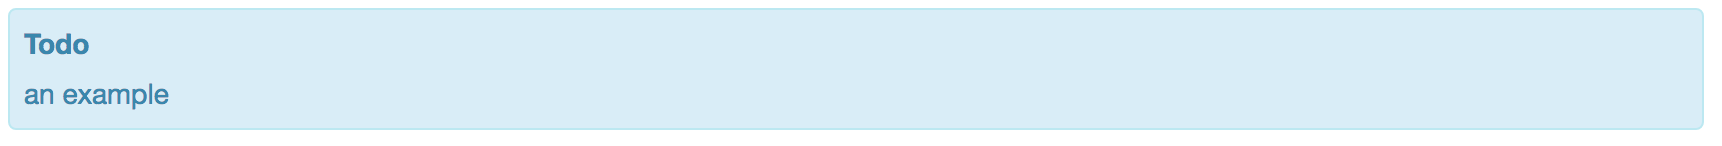
\includegraphics[width=\columnwidth]{../../images/todo.png}

\FILENAME

\section{Markdown}\label{markdown}

The content form this section originates from see:
\url{https://en.wikipedia.org/wiki/Markdown}.

Markdown is a simple markup language, however there is no precise
standard defined for it and implementations may have features not
supported by other implementations. Nevertheless, it provieds as imple
and easy way to quicly develop clean looking documents.

There are severla tools that make markdown attractive allowing to
write the text in one window while at the same time seeing the
rendered out put in another.

This includes

\begin{description}

\item[Macdown] An editor for mardown targeted on OSX

\end{description}

To convert the markdown to other formats with \verb|pandoc|

\begin{verbatim}
# Heading

## Sub-heading

### Another deeper heading
 
Paragraphs are separated
by a blank line.

Two spaces at the end of a line leave a  
line break.

Text attributes _italic_, *italic*, __bold__, **bold**, `monospace`.

Horizontal rule:

---

Bullet list:

  * apples
  * oranges
  * pears

Numbered list:

  1. apples
  2. oranges
  3. pears

A [link](http://example.com).

\end{verbatim}
\begin{fileremark}\url{https://github.com/cloudmesh/classes/blob/master/docs/source/lesson/doc/type.rst}\end{fileremark}
\section{Communicating Research in Other Ways}\label{communicating-research}

Naturally, writing papers is not the only way to communicate your
research with others. We find that today we see additional pathways
for cumminication includine blogs, twitter, facebook, e-mail, Web
pages, and electronic notebooks. Let us refisit some of them and
identify when they are helpful.

\subsection{Blogs}\label{blogs}

\begin{description}
\item[blog:]
noun, a regularly updated website or web page, typically one run by an
individual or small group, that is written in an informal or
conversational style.
\end{description}

Advantages:

\begin{itemize}
\tightlist
\item
  encourages spontaneous posts
\item
  encourages small short contributions
\item
  chronologically ordered
\item
  standard software exists to set up blogs
\item
  online services exists to set up blogs
\end{itemize}

Disadvantages:

\begin{itemize}
\tightlist
\item
  structuring data is difficult (some blog software support it)
\item
  not suitable for formal development of a paper
\item
  often lack of sophisticated track change features
\item
  no collaborative editing features
\end{itemize}

\subsection{Sphinx}\label{sphinx}

Sphinx (\url{http://www.sphinx-doc.org/}) is a tool that to create
integrated documentation from a markup language whlie.

Advantages:

\begin{itemize}
\tightlist
\item
  output formats: html, LaTeX, PDF, ePub
\item
  integrates well with directory structure
\item
  powerful markup language (reStructuredText)
\item
  can be hosted on github via github pages
\item
  can integare other renderers such as Markdown
\item
  automatic table of content, tebale of index
\item
  code documentation integration
\item
  search
\item
  written in python and using bash, so extensions and custom automation
  are possible
\end{itemize}

Disadvantage:

\begin{itemize}
\tightlist
\item
  requires compile step
\item
  When using markdown github can render individual page
\end{itemize}

Others:

\begin{itemize}
\tightlist
\item
  Read the Docs (\url{https://readthedocs.org/})
\item
  Doxygen (\url{http://www.stack.nl/~dimitri/doxygen/})
\item
  MkDocs (\url{http://www.mkdocs.org/})
\end{itemize}

\subsection{Notebooks}\label{notebooks}

\subsubsection{Jupyter}\label{jupyter}

The Jupyter Notebook (\url{http://jupyter.org/}) is an open-source web
application allowing users to create and share documents that contain
live code, equations, visualizations and explanatory text. Use cases
include data cleaning and transformation, numerical simulation,
statistical modeling, machine learning.

Advantages:

\begin{itemize}
\tightlist
\item
  Integrates with python
\item
  Recently other programming languages have been integrated
\item
  Allows experimenting with settings
\item
  Allows a form of literate programming while mixing documentation with
  code
\item
  automatically renders on github
\item
  comes with web service that allows hosting
\end{itemize}

Disadvantage:

\begin{itemize}
\tightlist
\item
  mostly encourages short documents
\item
  mark up language is limited
\item
  editing in ASCII is complex and Web editing is prefered
\end{itemize}

\subsubsection{Apache Zeppilin}\label{apache-zeppilin}

A Web-based notebook that enables data-driven, interactive data
analytics and collaborative documents with SQL, Scala and hadoop. It
integrates a web-based notebook with data ingestion, data exploration,
visualization, sharing and collaboration features to Hadoop and Spark.

Advantages:

\begin{itemize}
\tightlist
\item
  integration to various framework
\item
  Web framework
\item
  integration with spark, hadoop
\end{itemize}

Disadvantages:

\begin{itemize}
\tightlist
\item
  larger framework
\item
  must leverages existing deployments of spak, hadoop
\end{itemize}


\begin{comment}
\subsection{References}\label{references}

Collaboratories:

\begin{itemize}
\tightlist
\item
  Myers JD, TC Allison, SJ Bittner, BT Didier, M Frenklach, WH Green, YL
  Ho, J Hewson, WS Koegler, CS Lansing, D Leahy, M Lee, R McCoy, M
  Minkoff, S Nijsure, G von Laszewski, D Montoya, L Oluwole, CM
  Pancerella, R Pinzon, W Pitz, LA Rahn, B Ruscic, KL Schuchardt, EG
  Stephan, A Wagner, TL Windus, and C Yang. 2005. ``A Collaborative
  Informatics Infrastructure for Multi-scale Science.'' Cluster
  Computing 8(4):243-253.
\item
  Metadata in the Collaboratory for Multi-Scale Chemical Science Carmen
  Pancerella, John Hewson, Wendy Koegler, David Leahy, Michael Lee,
  Larry Rahn, Christine Yang, James D. Myers, Brett Didier, Renata
  McCoy, Karen Schuchardt, Eric Stephan, Theresa Windus, Kaizar Amin,
  Sandra Bittner, Carina Lansing, Michael Minkoff, Sandeep Nijsure,
  Gregor von Laszewski, Reinhardt Pinzon, Branko Ruscic, Al Wagner,
  Baoshan Wang, William Pitz, Yen-Ling Ho, David Montoya, Lili Xu,
  Thomas C. Allison, William H. Green, Jr., Michael Frenklach
  \url{http://dcpapers.dublincore.org/pubs/article/view/740/736}
\end{itemize}
\end{comment}


%----------------------------------------------------------------------------------------
%	PART
%----------------------------------------------------------------------------------------

\part{Big Data Applications}

\begin{fileremark}\currfiledir \currfilename\end{fileremark}

\section{Introduction}\label{introduction}

\begin{description}
\item[You may find that some videos may have a different lesson,]
section or unit number. Please ignore this. In case the content does not
correspond to the title, please let us know.
\end{description}

This section has a technical overview of course followed by a broad
motivation for course hosted at www-cloudmesh-classes.

The course overview covers it's content and structure. It presents an
introduction to general field of Big Data and Analytics. We are
especially analysing the many different application areas in which Big
Data can be applied. As Big Datais typically not just used in isolation
but is part of a larger Informatics issue for a particular field we also
use the term X-Informatics, where X defines a usecase or area of
specialization in which Big Data is applied to. As such we organize the
class around the the \emph{Rallying Cry} of course: Use Clouds running
Data Analytics Collaboratively processing Big Data to solve problems in
X-Informatics.

The courses is set up as a number of lessons that are typically between
20 minutes to an hour. The lessons are either provided as written
documents or as video lectures. They are enhanced by an in person
meeting that takes place either in a lecture room for residential
students or as online meeting for online students.

The course covers a mix of applications (the X in X-Informatics) and
technologies needed to support the field electronically i.e. to process
the application data. The overview ends with a discussion of course
content at highest level. The course starts with a motivation
summarizing clouds and data science, then units describing applications
in areas such as Physics, e-Commerce, Web Search and Text mining,
Health, Sensors and Remote Sensing). These are interspersed with
discussions of infrastructure (clouds) and data analytics (algorithms
like clustering and collaborative filtering used in applications). The
course uses Python as primary programming language. We will be
introducing practical use of cloud resources so that you have the
oportunity to explore example analytics applications on smaller data
sets that you define.

The course motivation starts with striking examples of the data deluge
with examples from research, business and the consumer. The growing
number of jobs in data science is highlighted. He describes industry
trend in both clouds and big data. Then the cloud computing model
developed at amazing speed by industry is introduced. The 4 paradigms of
scientific research are described with growing importance of data
oriented version.He covers 3 major X-informatics areas: Physics,
e-Commerce and Web Search followed by a broad discussion of cloud
applications. Parallel computing in general and particular features of
MapReduce are described.

We discuss in this course include the following topics. We may change
the order of the topics to allow for maximal flexibility and parallel
learning experiences.

Writing Track:

\begin{itemize}
\item  Writing a short review article
\item  Writing a porject or term report
\end{itemize}

Theory Track:

\begin{itemize}
\item  Motivation: Big Data and the Cloud; Centerpieces of the Future Economy
\item  Introduction: What is Big Data, Data Analytics
\item  Use Cases: Big Data Use Cases Survey

  \begin{itemize}
  \item    Use Case, Physics Discovery of Higgs Particle
  \item    Use Case: e-Commerce and Lifestyle with recommender systems
  \item    Use Case: Web Search and Text Mining and their technologies
  \item    Use Case: Sports
  \item    Use Case: Health
  \item    Use Case: Sensors
  \item    Use Case: Radar for Remote Sensing.
  \end{itemize}

\item Parallel Computing Overview and familiar examples
\item Cloud Technology for Big Data Applications \& Analytics
\end{itemize}

Practice Track:

\begin{itemize}
\item
  Python for Big Data Applications and Analytics: NumPy, SciPy,
  MatPlotlib
\item
  Using FutureGrid for Big Data Applications and Analytics Course
\item
  Using Chameleon Cloud for Big Data Applications and Analytics Course
\item
  {[}optional{]} Using Plotviz Software for Displaying Point
  Distributions in 3D
\item
  Recommender Systems - K-Nearest Neighbors, Clustering and heuristic
  methods
\item
  PageRank
\item
  Kmeans
\item
  MapReduce
\item
  Kmeans and MapReduce Parallelism
\end{itemize}

\subsection{Course Motivation}\label{course-motivation}

We motivate the study of X-informatics by describing data science and
clouds. He starts with striking examples of the data deluge with
examples from research, business and the consumer. The growing number of
jobs in data science is highlighted. He describes industry trend in both
clouds and big data.

He introduces the cloud computing model developed at amazing speed by
industry. The 4 paradigms of scientific research are described with
growing importance of data oriented version. He covers 3 major
X-informatics areas: Physics, e-Commerce and Web Search followed by a
broad discussion of cloud applications. Parallel computing in general
and particular features of MapReduce are described. He comments on a
data science education and the benefits of using MOOC's.

\subsubsection{Emerging Technologies}\label{emerging-technologies}

This presents the overview of talk, some trends in computing and data
and jobs. Gartner's emerging technology hype cycle shows many areas of
Clouds and Big Data. We highlight 6 issues of importance: economic
imperative, computing model, research model, Opportunities in advancing
computing, Opportunities in X-Informatics, Data Science Education


\video{Introduction}{40:14}{Motivation}  {https://drive.google.com/file/d/0B1Of61fJF7WsV2RvMlFzSDNPZEU/view?usp=sharing}
  
\slides{Introduction}{30}  {Motivation}{https://drive.google.com/file/d/0B8936_ytjfjmOUZraHc4M1ptczA/view?usp=sharing}


\subsubsection{Data Deluge}\label{data-deluge}

We give some amazing statistics for total storage; uploaded video and
uploaded photos; the social media interactions every minute; aspects of
the business big data tidal wave; monitors of aircraft engines; the
science research data sizes from particle physics to astronomy and earth
science; genes sequenced; and finally the long tail of science. The next
slide emphasizes applications using algorithms on clouds. This leads to
the rallying cry ``Use Clouds running Data Analytics Collaboratively
processing Big Data to solve problems in X-Informatics educated in data
science'`with a catalog of the many values of X''Astronomy, Biology,
Biomedicine, Business, Chemistry, Climate, Crisis, Earth Science,
Energy, Environment, Finance, Health, Intelligence, Lifestyle,
Marketing, Medicine, Pathology, Policy, Radar, Security, Sensor, Social,
Sustainability, Wealth and Wellness''


\video{Introduction}{30:38}  {Data Deluge}{https://www.youtube.com/watch?v=7VHPXJv3DN4}


\slides{Introduction}{20}  {Data  Deluge}{https://drive.google.com/open?id=0B8936_ytjfjmUXY3anBaeU9lLVU}

\subsubsection{Jobs}\label{jobs}

Jobs abound in clouds and data science. There are documented shortages
in data science, computer science and the major tech companies advertise
for new talent.


\video{Introduction}{9:39}  {Jobs}{https://www.youtube.com/watch?v=KsjiQS8uXDA}


\slides{Introduction}{8}  {Jobs}{https://drive.google.com/open?id=0B8936_ytjfjmaG50YW9TeWdvUTg}


\subsubsection{Industrial Trends}\label{industrial-trends}

Trends include the growing importance of mobile devices and comparative
decrease in desktop access, the export of internet content, the change
in dominant client operating systems, use of social media, thriving
Chinese internet companies.


\video{Introduction}{19:25} 
  {Industrial Trends}{https://www.youtube.com/watch?v=32vD7uN7fqY}


\slides{Introduction}{16}
  {Industrial
  Trends}{https://drive.google.com/open?id=0B8936_ytjfjmWW1SdXgxWkRLYjg}



\video{Introduction}{16:54}   {Industrial Trends  II}{https://www.youtube.com/watch?v=O8fgXAQcnvw}

\slides{Introduction}{16}
  {Indusrial
  Trends II}{https://drive.google.com/open?id=0B8936_ytjfjmeEV2R19ORzhBQVE}



\video{Introduction}{30:13} 
  {Indusrial Trends
  III}{https://www.youtube.com/watch?v=kW38MG7ukzs}

\slides{Introduction}{21}
  {Industrial
  Trends III}{https://drive.google.com/open?id=0B8936_ytjfjmNDZKcE1MSU45ZG8}


\subsubsection{Digital Disruption of Old
Favorites}\label{digital-disruption-of-old-favorites}

Not everything goes up. The rise of the Internet has led to declines in
some traditional areas including Shopping malls and Postal Services.

\video{Introduction}{32:54} 
{Digital Distruption
and transformation}{https://www.youtube.com/watch?v=bw9yYXwe7Bs} 



\slides{Introduction}{28}
  {Digital
  Distruption and transformation}{https://drive.google.com/open?id=0B8936_ytjfjmdW5CYnBtME9FVTQ}


\subsubsection{Computing Model}\label{computing-model}

\emph{Industry adopted clouds which are attractive for data analytics}

Clouds and Big Data are transformational on a 2-5 year time scale.
Already Amazon AWS is a lucrative business with almost a \$4B revenue.
We describe the nature of cloud centers with economies of scale and
gives examples of importance of virtualization in server consolidation.
Then key characteristics of clouds are reviewed with expected high
growth in Infrastructure, Platform and Software as a Service.


\video{Introduction}{24:03} 
  {Computing Model I}{https://www.youtube.com/watch?v=oYKTCKFGTco}


\slides{Introduction}{14}
  {Computing
  Model I}{https://drive.google.com/open?id=0B8936_ytjfjmTU9nNml2bUlsUHM}



\video{Introduction}{28:18} 
  {Computing Model II}{https://www.youtube.com/watch?v=km_eXHq7m3o}


\slides{Introduction}{27}
  {Computing
  Model II}{https://drive.google.com/open?id=0B8936_ytjfjmNHhLYnI0X0YxdFE}

\subsubsection{Research Model}\label{research-model}

\emph{4th Paradigm; From Theory to Data driven science?}

We introduce the 4 paradigms of scientific research with the focus on
the new fourth data driven methodology.


\video{Introduction}{7:33}  {Research Model}{https://www.youtube.com/watch?v=xkeECe3mmjI}


\slides{Introduction}{4}  {Research  Model}{https//drive.google.com/open?id=0B8936_ytjfjma0pMbHJnek02dDA}


\subsubsection{Data Science Process}\label{data-science-process}

We introduce the DIKW data to information to knowledge to wisdom
paradigm. Data flows through cloud services transforming itself and
emerging as new information to input into other transformations.


\video{Introduction}{15:42} {Data Science Process}{https://www.youtube.com/watch?v=KstIH2aQ60Y}


\slides{Introduction}{10}
  {Data  Science Process}{https://drive.google.com/open?id=0B8936_ytjfjmVDVZa01keW0wQmc}


\subsubsection{Physics-Informatics}\label{physics-informatics}

\emph{Looking for Higgs Particle with Large Hadron Collider LHC}

We look at important particle physics example where the Large hadron
Collider has observed the Higgs Boson. He shows this discovery as a bump
in a histogram; something that so amazed him 50 years ago that he got a
PhD in this field. He left field partly due to the incredible size of
author lists on papers.


\video{Introduction}{13:27} 
  {Physics-informatics}{https://www.youtube.com/watch?v=2A7Z741FCHs}

\slides{Introduction}{6}
  {Physics-inforamtics}{https://drive.google.com/open?id=0B8936_ytjfjmc2J2TWgwWGRwaFk}


\subsubsection{Recommender Systems}\label{recommender-systems}

Many important applications involve matching users, web pages, jobs,
movies, books, events etc. These are all optimization problems with
recommender systems one important way of performing this optimization.
We go through the example of Netflix \textasciitilde{}\textasciitilde{}
everything is a recommendation and muses about the power of viewing all
sorts of things as items in a bag or more abstractly some space with
funny properties.


\video{Introduction}{12:21}
  {Recommender Systems  I}{https://www.youtube.com/watch?v=LXhng3fcG9o}



\slides{Introduction}{9}
  {Recommender  Systems I}{https://drive.google.com/open?id=0B8936_ytjfjmOXlVd2FsSUkwekk}



\video{Introduction}{9:44} 
  {Recommender Systems
  II}{https://www.youtube.com/watch?v=Y4S0jY0yfEE}

\slides{Introduction}{6}
  {Recommender
  Systems II}{https://drive.google.com/open?id=0B8936_ytjfjmMzM2M3RhMEJ4bjQ}


\subsubsection{Web Search and Information
Retrieval}\label{web-search-and-information-retrieval}

This course also looks at Web Search and here we give an overview of the
data analytics for web search, Pagerank as a method of ranking web pages
returned and uses material from Yahoo on the subtle algorithms for
dynamic personalized choice of material for web pages.


\video{Introduction}{12:05}   {Web Search and  Information Retrieval}{https://www.youtube.com/watch?v=p-0NtNTzoh8}


\slides{Introduction}{6}  {Web  Search and Information Retrieval}{https://drive.google.com/open?id=0B8936_ytjfjmSm8zNmZ5VFJxRms}


\subsubsection{Cloud Application in
Research}\label{cloud-application-in-research}

We describe scientific applications and how they map onto clouds,
supercomputers, grids and high throughput systems. He likes the cloud
use of the Internet of Things and gives examples.


\video{Introduction}{33:51}{Cloud Applications  in Research}{https://www.youtube.com/watch?v=U3ZG2qOFpxE}


\slides{Introduction}{20}  {Cloud  Applications in Research}{https://drive.google.com/open?id=0B8936_ytjfjma0RhdU0zdkxmczA}

\subsubsection{Parallel Computing and
MapReduce}\label{parallel-computing-and-mapreduce}

We define MapReduce and gives a homely example from fruit blending.


\video{Introduction}{14:02}  {Computing and  MapReduce}{https://www.youtube.com/watch?v=aQ8NMxe9IsU}


\slides{Introduction}{9}  {Computing  and MapReduce}{https://drive.google.com/open?id=0B8936_ytjfjmeTl4NWhHRjJMOGc}

\subsubsection{Data Science Education}\label{data-science-education}

We discuss one reason you are taking this course
\textasciitilde{}\textasciitilde{} Data Science as an educational
initiative and aspects of its Indiana University implementation. Then
general; features of online education are discussed with clear growth
spearheaded by MOOC's where we use this course and others as an example.
He stresses the choice between one class to 100,000 students or 2,000
classes to 50 students and an online library of MOOC lessons. In olden
days he suggested `'hermit's cage virtual university''
\textasciitilde{}\textasciitilde{} gurus in isolated caves putting
together exciting curricula outside the traditional university model.
Grading and mentoring models and important online tools are discussed.
Clouds have MOOC's describing them and MOOC's are stored in clouds; a
pleasing symmetry.


\video{Introduction}{28:08}   {Data Science  Education}{https://www.youtube.com/watch?v=bA_eNjJTmRQ}


\slides{Introduction}{19}  {Data  Science Education}{https://drive.google.com/open?id=0B8936_ytjfjmT0J1RjYwY1VwZ1k}


\subsubsection{Conclusions}\label{conclusions}

The conclusions highlight clouds, data-intensive methodology,
employment, data science, MOOC's and never forget the Big Data ecosystem
in one sentence ``Use Clouds running Data Analytics Collaboratively
processing Big Data to solve problems in X-Informatics educated in data
science''


\video{Introduction}{4:59}  {Conclusions}{https://www.youtube.com/watch?v=FmcR5mrhYvk}

\slides{Introduction}{4}  {Conclusions}{https://drive.google.com/open?id=0B8936_ytjfjmVjRNeG1pdUNnMlE}


\subsubsection{Resources}\label{resources}

\begin{itemize}
\item
  \url{http://www.gartner.com/technology/home.jsp} and many web links
\item
  Meeker/Wu May 29 2013 Internet Trends D11 Conference
  \url{http://www.slideshare.net/kleinerperkins/kpcb-internet-trends-2013}
\item
  \url{http://cs.metrostate.edu/~sbd/slides/Sun.pdf}
\item
  Taming The Big Data Tidal Wave: Finding Opportunities in Huge Data
  Streams with Advanced Analytics, Bill Franks Wiley ISBN:
  978-1-118-20878-6
\item
  Bill Ruh
  \url{http://fisheritcenter.haas.berkeley.edu/Big_Data/index.html}
\item
  \url{http://www.genome.gov/sequencingcosts/}
\item
  CSTI General Assembly 2012, Washington, D.C., USA Technical Activities
  Coordinating Committee (TACC) Meeting, Data Management, Cloud
  Computing and the Long Tail of Science October 2012 Dennis Gannon
\item
  \url{http://www.microsoft.com/en-us/news/features/2012/mar12/03-05CloudComputingJobs.aspx}
\item
  \url{http://www.mckinsey.com/mgi/publications/big_data/index.asp}
\item
  Tom Davenport
  \url{http://fisheritcenter.haas.berkeley.edu/Big_Data/index.html}
\item
  \url{http://research.microsoft.com/en-us/people/barga/sc09_cloudcomp_tutorial.pdf}
\item
  \url{http://research.microsoft.com/pubs/78813/AJ18_EN.pdf}
\item
  \url{http://www.google.com/green/pdfs/google-green-computing.pdf}
\item
  \url{http://www.wired.com/wired/issue/16-07}
\item
  \url{http://research.microsoft.com/en-us/collaboration/fourthparadigm/}
\item
  Jeff Hammerbacher
  \url{http://berkeleydatascience.files.wordpress.com/2012/01/20120117berkeley1.pdf}
\item
  \url{http://grids.ucs.indiana.edu/ptliupages/publications/Where\%20does\%20all\%20the\%20data\%20come\%20from\%20v7.pdf}
\item
  \url{http://www.interactions.org/cms/?pid=1032811}
\item
  \url{http://www.quantumdiaries.org/2012/09/07/why-particle-detectors-need-a-trigger/atlasmgg/}
\item
  \url{http://www.sciencedirect.com/science/article/pii/S037026931200857X}
\item
  \url{http://www.slideshare.net/xamat/building-largescale-realworld-recommender-systems-recsys2012-tutorial}
\item
  \url{http://www.ifi.uzh.ch/ce/teaching/spring2012/16-Recommender-Systems_Slides.pdf}
\item
  \url{http://en.wikipedia.org/wiki/PageRank}
\item
  \url{http://pages.cs.wisc.edu/~beechung/icml11-tutorial/}
\item
  \url{https://sites.google.com/site/opensourceiotcloud/}
\item
  \url{http://datascience101.wordpress.com/2013/04/13/new-york-times-data-science-articles/}
\item
  \url{http://blog.coursera.org/post/49750392396/on-the-topic-of-boredom}
\item
  \url{http://x-informatics.appspot.com/course}
\item
  \url{http://iucloudsummerschool.appspot.com/preview}
\item
  \url{https://www.youtube.com/watch?v=M3jcSCA9_hM}
\end{itemize}



%\begin{fileremark}\currfiledir \currfilename\end{fileremark}

\section{Overview of Data Science}\label{overview-of-data-science}

\emph{What is Big Data, Data Analytics and X-Informatics?}

The course introduction starts with X-Informatics and its rallying cry.
The growing number of jobs in data science is highlighted. The first
unit offers a look at the phenomenon described as the Data Deluge
starting with its broad features. Data science and the famous DIKW (Data
to Information to Knowledge to Wisdom) pipeline are covered. Then more
detail is given on the flood of data from Internet and Industry
applications with eBay and General Electric discussed in most detail.

In the next unit, we continue the discussion of the data deluge with a
focus on scientific research. He takes a first peek at data from the
Large Hadron Collider considered later as physics Informatics and gives
some biology examples. He discusses the implication of data for the
scientific method which is changing with the data-intensive methodology
joining observation, theory and simulation as basic methods. Two broad
classes of data are the long tail of sciences: many users with
individually modest data adding up to a lot; and a myriad of Internet
connected devices -- the Internet of
Things.

We give an initial technical overview of cloud computing as pioneered by
companies like Amazon, Google and Microsoft with new centers holding up
to a million servers. The benefits of Clouds in terms of power
consumption and the environment are also touched upon, followed by a
list of the most critical features of Cloud computing with a comparison
to supercomputing. Features of the data deluge are discussed with a
salutary example where more data did better than more thought. Then
comes Data science and one part of it \textasciitilde{}\textasciitilde{}
data analytics \textasciitilde{}\textasciitilde{} the large algorithms
that crunch the big data to give big wisdom. There are many ways to
describe data science and several are discussed to give a good composite
picture of this emerging field.

\subsection{Data Science generics and Commercial Data
Deluge}\label{data-science-generics-and-commercial-data-deluge}

We start with X-Informatics and its rallying cry. The growing number of
jobs in data science is highlighted. This unit offers a look at the
phenomenon described as the Data Deluge starting with its broad
features. Then he discusses data science and the famous DIKW (Data to
Information to Knowledge to Wisdom) pipeline. Then more detail is given
on the flood of data from Internet and Industry applications with eBay
and General Electric discussed in most detail.


\slides{Overview}{45}{TBD}{https://drive.google.com/open?id=0B88HKpainTSfenJ4dEZQOUxZSmM}


\subsubsection{What is X-Informatics and its
Motto}\label{what-is-x-informatics-and-its-motto}

This discusses trends that are driven by and accompany Big data. We give
some key terms including data, information, knowledge, wisdom, data
analytics and data science. WE introduce the motto of the course: Use
Clouds running Data Analytics Collaboratively processing Big Data to
solve problems in X-Informatics. We list many values of X you can
defined in various activities across the world.


\video{Overview}{9:49}{TBD}{https://www.youtube.com/watch?v=8T0OtdR9Bp4}




\subsubsection{Jobs}\label{jobs}

Big data is especially important as there are some many related jobs. We
illustrate this for both cloud computing and data science from reports
by Microsoft and the McKinsey institute respectively. We show a plot
from LinkedIn showing rapid increase in the number of data science and
analytics jobs as a function of time.


\video{Overview}{2:58}{TBD}{http://youtu.be/pRlfEigUJAc}

\subsubsection{Data Deluge: General
Structure}\label{data-deluge-general-structure}

We look at some broad features of the data deluge starting with the size
of data in various areas especially in science research. We give
examples from real world of the importance of big data and illustrate
how it is integrated into an enterprise IT architecture. We give some
views as to what characterizes Big data and why data science is a
science that is needed to interpret all the data.


\video{Overview}{13:04}{TBD}{http://youtu.be/mPJ9twAFRQU}

\subsubsection{Data Science: Process}\label{data-science-process}

We stress the DIKW pipeline: Data becomes information that becomes
knowledge and then wisdom, policy and decisions. This pipeline is
illustrated with Google maps and we show how complex the ecosystem of
data, transformations (filters) and its derived forms is.


\video{Overview}{4:27}{TBD}{http://youtu.be/ydH34L-z0Rk}

\subsubsection{Data Deluge: Internet}\label{data-deluge-internet}

We give examples of Big data from the Internet with Tweets, uploaded
photos and an illustration of the vitality and size of many commodity
applications.


\video{Overview}{3:42}{TBD}{http://youtu.be/rtuq5y2Bx2g}

\subsubsection{Data Deluge: Business}\label{data-deluge-business}

We give examples including the Big data that enables wind farms, city
transportation, telephone operations, machines with health monitors, the
banking, manufacturing and retail industries both online and offline in
shopping malls. We give examples from ebay showing how analytics
allowing them to refine and improve the customer experiences.


\video{Overview}{6:00}{TBD}{http://youtu.be/PJz38t6yn_s}

\video{Overview}{7:34}{TBD}{http://youtu.be/fESm-2Vox9M}

\video{Overview}{9:37}{TBD}{http://youtu.be/fcvn-IxPO00}

\subsubsection{Resources}\label{resources}

\begin{itemize}
\item
  \url{http://www.microsoft.com/en-us/news/features/2012/mar12/03-05CloudComputingJobs.aspx}
\item
  \url{http://www.mckinsey.com/mgi/publications/big_data/index.asp}
\item
  Tom Davenport
  \url{http://fisheritcenter.haas.berkeley.edu/Big_Data/index.html}
\item
  Anjul Bhambhri
  \url{http://fisheritcenter.haas.berkeley.edu/Big_Data/index.html}
\item
  Jeff Hammerbacher
  \url{http://berkeleydatascience.files.wordpress.com/2012/01/20120117berkeley1.pdf}
\item
  \url{http://www.economist.com/node/15579717}
\item
  \url{http://cs.metrostate.edu/~sbd/slides/Sun.pdf}
\item
  \url{http://jess3.com/geosocial-universe-2/}
\item
  Bill Ruh \url{http://fisheritcenter.haas.berkeley.edu/Big\_Data/index.html}
\item
  \url{http://www.hsph.harvard.edu/ncb2011/files/ncb2011-z03-rodriguez.pptx}
\item
  Hugh Williams
  \url{http://fisheritcenter.haas.berkeley.edu/Big_Data/index.html}
\end{itemize}

\subsection{Data Deluge and Scientific Applications and
Methodology}\label{data-deluge-and-scientific-applications-and-methodology}

\subsubsection{Overview}\label{overview}

We continue the discussion of the data deluge with a focus on scientific
research. He takes a first peek at data from the Large Hadron Collider
considered later as physics Informatics and gives some biology examples.
He discusses the implication of data for the scientific method which is
changing with the data-intensive methodology joining observation, theory
and simulation as basic methods. We discuss the long tail of sciences;
many users with individually modest data adding up to a lot. The last
lesson emphasizes how everyday devices
\textasciitilde{}\textasciitilde{} the Internet of Things
\textasciitilde{}\textasciitilde{} are being used to create a wealth of
data.

\slides{Overview}{22}{TBD}{https://drive.google.com/open?id=0B88HKpainTSfZzhqZHVKbllZcTA}{PDF}


\subsubsection{Science \& Research}\label{science-research}

We look into more big data examples with a focus on science and
research. We give astronomy, genomics, radiology, particle physics and
discovery of Higgs particle (Covered in more detail in later lessons),
European Bioinformatics Institute and contrast to Facebook and Walmart.


\video{Overview}{11:27}{TBD}{http://youtu.be/u1h6bAkuWQ8}

\video{Overview}{11:49}{TBD}{http://youtu.be/_JfcUg2cheg}


\subsubsection{Implications for Scientific
Method}\label{implications-for-scientific-method}

We discuss the emergences of a new fourth methodology for scientific
research based on data driven inquiry. We contrast this with third
\textasciitilde{}\textasciitilde{} computation or simulation based
discovery - methodology which emerged itself some 25 years ago.


\video{Overview}{5:07}{TBD}{http://youtu.be/srEbOAmU_g8}

\subsubsection{Long Tail of Science}\label{long-tail-of-science}

There is big science such as particle physics where a single experiment
has 3000 people collaborate!.Then there are individual investigators who
don't generate a lot of data each but together they add up to Big data.


\video{Overview}{2:10}{TBD}{http://youtu.be/dwzEKEGYhqE}

\subsubsection{Internet of Things}\label{internet-of-things}

A final category of Big data comes from the Internet of Things where
lots of small devices \textasciitilde{}\textasciitilde{} smart phones,
web cams, video games collect and disseminate data and are controlled
and coordinated in the cloud.


\video{Overview}{5:45}{TBD}{http://youtu.be/K2anbyxX48w}


\subsubsection{Resources}\label{resources-1}

\begin{itemize}
\tightlist
\item
  \url{http://www.economist.com/node/15579717}
\item
  Geoffrey Fox and Dennis Gannon Using Clouds for Technical Computing To
  be published in Proceedings of HPC 2012 Conference at Cetraro, Italy
  June 28 2012
\item
  \url{http://grids.ucs.indiana.edu/ptliupages/publications/Clouds_Technical_Computing_FoxGannonv2.pdf}
\item
  \url{http://grids.ucs.indiana.edu/ptliupages/publications/Where\%20does\%20all\%20the\%20data\%20come\%20from\%20v7.pdf}
\item
  \url{http://www.genome.gov/sequencingcosts/}
\item
  \url{http://www.quantumdiaries.org/2012/09/07/why-particle-detectors-need-a-trigger/atlasmgg}
\item
  \url{http://salsahpc.indiana.edu/dlib/articles/00001935/}
\item
  \url{http://en.wikipedia.org/wiki/Simple_linear_regression}
\item
  \url{http://www.ebi.ac.uk/Information/Brochures/}
\item
  \url{http://www.wired.com/wired/issue/16-07}
\item
  \url{http://research.microsoft.com/en-us/collaboration/fourthparadigm/}
\item
  CSTI General Assembly 2012, Washington, D.C., USA Technical Activities
  Coordinating Committee (TACC) Meeting, Data Management, Cloud
  Computing and the Long Tail of Science October 2012 Dennis Gannon
  \url{https://sites.google.com/site/opensourceiotcloud/}
\end{itemize}

\subsection{Clouds and Big Data Processing; Data Science Process and
Analytics}\label{clouds-and-big-data-processing-data-science-process-and-analytics}

\subsubsection{Overview}\label{overview-1}

We give an initial technical overview of cloud computing as pioneered by
companies like Amazon, Google and Microsoft with new centers holding up
to a million servers. The benefits of Clouds in terms of power
consumption and the environment are also touched upon, followed by a
list of the most critical features of Cloud computing with a comparison
to supercomputing.

He discusses features of the data deluge with a salutary example where
more data did better than more thought. He introduces data science and
one part of it \textasciitilde{}\textasciitilde{} data analytics
\textasciitilde{}\textasciitilde{} the large algorithms that crunch the
big data to give big wisdom. There are many ways to describe data
science and several are discussed to give a good composite picture of
this emerging field.


  \slides{Overview}{35}{TBD}{https://drive.google.com/open?id=0B88HKpainTSfV1FwdktnbTl3T1k}{PDF}


\subsection{Clouds}\label{clouds}

We describe cloud data centers with their staggering size with up to a
million servers in a single data center and centers built modularly from
shipping containers full of racks. The benefits of Clouds in terms of
power consumption and the environment are also touched upon, followed by
a list of the most critical features of Cloud computing and a comparison
to supercomputing.


\video{Overview}{16:04}{TBD}{https://www.youtube.com/watch?v=trIFW-rucgM}{MP4}



\subsubsection{Features of Data Deluge I}\label{features-of-data-deluge-i}

Data, Information, intelligence algorithms, infrastructure, data
structure, semantics and knowledge are related. The semantic web and Big
data are compared. We give an example where ``More data usually beats
better algorithms''. We discuss examples of intelligent big data and
list 8 different types of data deluge


\video{Overview}{8:02}{TBD}{http://youtu.be/FMktnTQGyrw}

\video{Overview}{6:24}{TBD}{http://youtu.be/QNVZobXHiZw}


\subsubsection{Data Science Process}\label{data-science-process-1}

We describe and critique one view of the work of a data scientists. Then
we discuss and contrast 7 views of the process needed to speed data
through the DIKW pipeline.


\video{Overview}{11:28}{TBD}{http://youtu.be/lpQ-Q9ZidR4}


\subsubsection{Data Analytics}\label{data-analytics}

\slides{Overview}{30}{TBD}{http://archive2.cra.org/ccc/files/docs/nitrdsymposium/keyes.pdf}


We stress the importance of data analytics giving examples from several
fields. We note that better analytics is as important as better
computing and storage capability. In the second video we look at High
Performance Computing in Science and Engineering: the Tree and the
Fruit.


\video{Overview}{7:28}{TBD}{http://youtu.be/RPVojR8jrb8}

\video{Overview}{6:51}{TBD}{http://youtu.be/wOSgywqdJDY}


\subsubsection{Resources}\label{resources-2}

\begin{itemize}
\tightlist
\item
  CSTI General Assembly 2012, Washington, D.C., USA Technical Activities
  Coordinating Committee (TACC) Meeting, Data Management, Cloud
  Computing and the Long Tail of Science October 2012 Dennis Gannon
\item
  Dan Reed Roger Barga Dennis Gannon Rich
  Wolskihttp://research.microsoft.com/en-us/people/barga/sc09\_cloudcomp\_tutorial.pdf
\item
  \url{http://www.datacenterknowledge.com/archives/2011/05/10/uptime-institute-the-average-pue-is-1-8/}
\item
  \url{http://loosebolts.wordpress.com/2008/12/02/our-vision-for-generation-4-modular-data-centers-one-way-of-getting-it-just-right/}
\item
  \url{http://www.mediafire.com/file/zzqna34282frr2f/koomeydatacenterelectuse2011finalversion.pdf}
\item
  Bina Ramamurthy
  \url{http://www.cse.buffalo.edu/~bina/cse487/fall2011/}
\item
  Jeff Hammerbacher
  \url{http://berkeleydatascience.files.wordpress.com/2012/01/20120117berkeley1.pdf}
\item
  Jeff Hammerbacher
  \url{http://berkeleydatascience.files.wordpress.com/2012/01/20120119berkeley.pdf}
\item
  Anjul Bhambhri
  \url{http://fisheritcenter.haas.berkeley.edu/Big_Data/index.html}
\item
  \url{http://cs.metrostate.edu/~sbd/slides/Sun.pdf}
\item
  Hugh Williams
  \url{http://fisheritcenter.haas.berkeley.edu/Big_Data/index.html}
\item
  Tom Davenport
  \url{http://fisheritcenter.haas.berkeley.edu/Big_Data/index.html}
\item
  \url{http://www.mckinsey.com/mgi/publications/big_data/index.asp}
\item
  \url{http://cra.org/ccc/docs/nitrdsymposium/pdfs/keyes.pdf}
\end{itemize}

\begin{fileremark}\url{https://github.com/cloudmesh/classes/blob/master/docs/source/i523/2017/course/health.rst}\end{fileremark}
\section{Health Informatics Case
Study}\label{health-informatics-case-study}

This section starts by discussing general aspects of Big Data and Health
including data sizes, different areas including genomics, EBI, radiology
and the Quantified Self movement. We review current state of health care
and trends associated with it including increased use of Telemedicine.
We summarize an industry survey by GE and Accenture and an impressive
exemplar Cloud-based medicine system from Potsdam. We give some details
of big data in medicine. Some remarks on Cloud computing and Health
focus on security and privacy issues.

We survey an April 2013 McKinsey report on the Big Data revolution in US
health care; a Microsoft report in this area and a European Union report
on how Big Data will allow patient centered care in the future. Examples
are given of the Internet of Things, which will have great impact on
health including wearables. A study looks at 4 scenarios for healthcare
in 2032. Two are positive, one middle of the road and one negative. The
final topic is Genomics, Proteomics and Information Visualization.

\subsection{X-Informatics Case Study: Health
Informatics}\label{x-informatics-case-study-health-informatics}

\subsubsection{Overview}\label{overview}

\slides{Health}{131}{https://drive.google.com/open?id=0B6wqDMIyK2P7UGRJNmlkYkNkQk0}

This section starts by discussing general aspects of Big Data and Health
including data sizes, different areas including genomics, EBI, radiology
and the Quantified Self movement. We review current state of health care
and trends associated with it including increased use of Telemedicine.
We summarize an industry survey by GE and Accenture and an impressive
exemplar Cloud-based medicine system from Potsdam. We give some details
of big data in medicine. Some remarks on Cloud computing and Health
focus on security and privacy issues.

We survey an April 2013 McKinsey report on the Big Data revolution in US
health care; a Microsoft report in this area and a European Union report
on how Big Data will allow patient centered care in the future. Examples
are given of the Internet of Things, which will have great impact on
health including wearables. A study looks at 4 scenarios for healthcare
in 2032. Two are positive, one middle of the road and one negative. The
final topic is Genomics, Proteomics and Information Visualization.

\subsubsection{Big Data and Health}\label{big-data-and-health}

This lesson starts with general aspects of Big Data and Health including
listing subareas where Big data important. Data sizes are given in
radiology, genomics, personalized medicine, and the Quantified Self
movement, with sizes and access to European Bioinformatics Institute.

\video{10:02}{Big Data and Health}{https://www.youtube.com/watch?v=ZkM-yZJQ1Cg} 

\subsubsection{Status of Healthcare
Today}\label{status-of-healthcare-today}

This covers trends of costs and type of healthcare with low cost genomes
and an aging population. Social media and government Brain initiative.

\video{16:09}{Status of Healthcare Today}{https://www.youtube.com/watch?v=x9TpdMBqYrk} 

\subsubsection{Telemedicine (Virtual
Health)}\label{telemedicine-virtual-health}

This describes increasing use of telemedicine and how we tried and
failed to do this in 1994.

\video{8:21}{Telemedicine}{https://www.youtube.com/watch?v=Pe4CVXQaL_U} 


\subsubsection{Big Data and Healthcare
Industry}\label{big-data-and-healthcare-industry}

Summary of an industry survey by GE and Accenture.

\video{10:02}{Big Data and Healthcare Indusry}{https://www.youtube.com/watch?v=64YOUnRJVZU}


\subsubsection{Medical Big Data in the
Clouds}\label{medical-big-data-in-the-clouds}

An impressive exemplar Cloud-based medicine system from Potsdam.

\video{15:02}{Medical Big Data in the Clouds}{https://www.youtube.com/watch?v=GldSVijkJcM} 


\subsubsection{Medical image Big Data}\label{medical-image-big-data}

\video{6:33}{Midical Image Big Data}{https://www.youtube.com/watch?v=GOcVtwx2R2k} 

\subsubsection{Clouds and Health}\label{clouds-and-health}

\video{4:35}{Clouds and Health}{http://youtu.be/9Whkl_UPS5g}


\subsubsection{McKinsey Report on the big-data revolution in US health
care}\label{mckinsey-report-on-the-big-data-revolution-in-us-health-care}

This lesson covers 9 aspects of the McKinsey report. These are the
convergence of multiple positive changes has created a tipping point for
innovation; Primary data pools are at the heart of the big data
revolution in healthcare; Big data is changing the paradigm: these are
the value pathways; Applying early successes at scale could reduce US
healthcare costs by \$300 billion to \$450 billion; Most new big-data
applications target consumers and providers across pathways; Innovations
are weighted towards influencing individual decision-making levers; Big
data innovations use a range of public, acquired, and proprietary data
types; Organizations implementing a big data transformation should
provide the leadership required for the associated cultural
transformation; Companies must develop a range of big data capabilities.

\video{14:53}{McKinsey Report}{https://www.youtube.com/watch?v=fu-TWnIk980} 

\subsubsection{Microsoft Report on Big Data in
Health}\label{microsoft-report-on-big-data-in-health}

This lesson identifies data sources as Clinical Data, Pharma \& Life
Science Data, Patient \& Consumer Data, Claims \& Cost Data and
Correlational Data. Three approaches are Live data feed, Advanced
analytics and Social analytics.

\video{2:26}{Microsoft Report on Big Data in Health}{http://youtu.be/PjffvVgj1PE}


\subsubsection{EU Report on Redesigning health in Europe for
2020}\label{eu-report-on-redesigning-health-in-europe-for-2020}

This lesson summarizes an EU Report on Redesigning health in Europe for
2020. The power of data is seen as a lever for change in My Data, My
decisions; Liberate the data; Connect up everything; Revolutionize
health; and Include Everyone removing the current correlation between
health and wealth.


\video{5:00}{EU Report on Redesigning health in Europe for 2020}{http://youtu.be/9mbt_ZSs0iw}


\subsubsection{Medicine and the Internet of
Things}\label{medicine-and-the-internet-of-things}

The Internet of Things will have great impact on health including
telemedicine and wearables. Examples are given.

\video{8:17}{Medicine and the Internet of Things}{https://www.youtube.com/watch?v=Jk3EeFzZnuU}


\subsubsection{Extrapolating to 2032}\label{extrapolating-to-2032}

A study looks at 4 scenarios for healthcare in 2032. Two are positive,
one middle of the road and one negative.

\video{15:13}{Extrapolating to 2032}{https://www.youtube.com/watch?v=a5G4HACeokg} 


\subsubsection{Genomics, Proteomics and Information
Visualization}\label{genomics-proteomics-and-information-visualization}

A study of an Azure application with an Excel frontend and a cloud BLAST
backend starts this lesson. This is followed by a big data analysis of
personal genomics and an analysis of a typical DNA sequencing analytics
pipeline. The Protein Sequence Universe is defined and used to motivate
Multi dimensional Scaling MDS. Sammon's method is defined and its use
illustrated by a metagenomics example. Subtleties in use of MDS include
a monotonic mapping of the dissimilarity function. The application to
the COG Proteomics dataset is discussed. We note that the MDS approach
is related to the well known chisq method and some aspects of nonlinear
minimization of chisq (Least Squares) are discussed.

\video{6:56}{Genomics, Proteomics and  Information Visualization}{https://www.youtube.com/watch?v=zGzBtxq1ZRE}

\video{6:56}{ CC) Genomics, Proteomics and  Information Visualization}{https://drive.google.com/file/d/0B5plU-u0wqMoVzduODM0Z2dFYWM/view?usp=sharing}


Next we continue the discussion of the COG Protein Universe introduced
in the last lesson. It is shown how Proteomics clusters are clearly seen
in the Universe browser. This motivates a side remark on different
clustering methods applied to metagenomics. Then we discuss the
Generative Topographic Map GTM method that can be used in dimension
reduction when original data is in a metric space and is in this case
faster than MDS as GTM computational complexity scales like N not N
squared as seen in MDS.

Examples are given of GTM including an application to topic models in
Information Retrieval. Indiana University has developed a deterministic
annealing improvement of GTM. 3 separate clusterings are projected for
visualization and show very different structure emphasizing the
importance of visualizing results of data analytics. The final slide
shows an application of MDS to generate and visualize phylogenetic
trees.

\video{10:33}{Genomics, Proteomics and Information Visualization I}{https://drive.google.com/file/d/0B5plU-u0wqMobXdEQWRHWl95UTA/view?usp=sharing}

\video{7:41}{Genomics, Proteomics and Information Visualization: II}{https://drive.google.com/file/d/0B5plU-u0wqModlhmdVUwdGlQNTA/view?usp=sharing}

\slides{Proteomics and Information Visualization}{131}{https://drive.google.com/open?id=0B8936_ytjfjmX0lEMWhMX2kwRHc}
  


\subsubsection{Resources}\label{resources}

\begin{itemize}
\tightlist
\item
  \url{https://wiki.nci.nih.gov/display/CIP/CIP+Survey+of+Biomedical+Imaging+Archives}
\item
  \url{http://grids.ucs.indiana.edu/ptliupages/publications/Where\%20does\%20all\%20the\%20data\%20come\%20from\%20v7.pdf}
\item
  \url{http://www.ieee-icsc.org/ICSC2010/Tony\%20Hey\%20-\%2020100923.pdf}
\item
  \url{http://quantifiedself.com/larry-smarr/}
\item
  \url{http://www.ebi.ac.uk/Information/Brochures/}
\item
  \url{http://www.kpcb.com/internet-trends}
\item
  \url{http://www.slideshare.net/drsteventucker/wearable-health-fitness-trackers-and-the-quantified-self}
\item
  \url{http://www.siam.org/meetings/sdm13/sun.pdf}
\item
  \url{http://en.wikipedia.org/wiki/Calico_\%28company\%29}
\item
  \url{http://www.slideshare.net/GSW_Worldwide/2015-health-trends}
\item
  \url{http://www.accenture.com/SiteCollectionDocuments/PDF/Accenture-Industrial-Internet-Changing-Competitive-Landscape-Industries.pdf}
\item
  \url{http://www.slideshare.net/schappy/how-realtime-analysis-turns-big-medical-data-into-precision-medicine}
\item
  \url{http://medcitynews.com/2013/03/the-body-in-bytes-medical-images-as-a-source-of-healthcare-big-data-infographic/}
\item
  \url{http://healthinformatics.wikispaces.com/file/view/cloud_computing.ppt}
\item
  \url{http://www.mckinsey.com/~/media/McKinsey/dotcom/Insights/Health\%20care/The\%20big-data\%20revolution\%20in\%20US\%20health\%20care/The\%20big-data\%20revolution\%20in\%20US\%20health\%20care\%20Accelerating\%20value\%20and\%20innovation.ashx}
\item
  \url{https://partner.microsoft.com/download/global/40193764}
\item
  \url{http://ec.europa.eu/information_society/activities/health/docs/policy/taskforce/redesigning_health-eu-for2020-ehtf-report2012.pdf}
\item
  \url{http://www.kpcb.com/internet-trends}
\item
  \url{http://www.liveathos.com/apparel/app}
\item
  \url{http://debategraph.org/Poster.aspx?aID=77}
\item
  \url{http://www.oerc.ox.ac.uk/downloads/presentations-from-events/microsoftworkshop/gannon}
\item
  \url{http://www.delsall.org}
\item
  \url{http://salsahpc.indiana.edu/millionseq/mina/16SrRNA_index.html}
\item
  \url{http://www.geatbx.com/docu/fcnindex-01.html}
\item
  \url{https://wiki.nci.nih.gov/display/CIP/CIP+Survey+of+Biomedical+Imaging+Archives}
\item
  \url{http://grids.ucs.indiana.edu/ptliupages/publications/Where\%20does\%20all\%20the\%20data\%20come\%20from\%20v7.pdf}
\item
  \url{http://www.ieee-icsc.org/ICSC2010/Tony\%20Hey\%20-\%2020100923.pdf}
\item
  \url{http://quantifiedself.com/larry-smarr/}
\item
  \url{http://www.ebi.ac.uk/Information/Brochures/}
\item
  \url{http://www.kpcb.com/internet-trends}
\item
  \url{http://www.slideshare.net/drsteventucker/wearable-health-fitness-trackers-and-the-quantified-self}
\item
  \url{http://www.siam.org/meetings/sdm13/sun.pdf}
\item
  \url{http://en.wikipedia.org/wiki/Calico_\%28company\%29}
\item
  \url{http://www.slideshare.net/GSW_Worldwide/2015-health-trends}
\item
  \url{http://www.accenture.com/SiteCollectionDocuments/PDF/Accenture-Industrial-Internet-Changing-Competitive-Landscape-Industries.pdf}
\item
  \url{http://www.slideshare.net/schappy/how-realtime-analysis-turns-big-medical-data-into-precision-medicine}
\item
  \url{http://medcitynews.com/2013/03/the-body-in-bytes-medical-images-as-a-source-of-healthcare-big-data-infographic/}
\item
  \url{http://healthinformatics.wikispaces.com/file/view/cloud_computing.ppt}
\item
  \url{http://www.mckinsey.com/~/media/McKinsey/dotcom/Insights/Health\%20care/The\%20big-data\%20revolution\%20in\%20US\%20health\%20care/The\%20big-data\%20revolution\%20in\%20US\%20health\%20care\%20Accelerating\%20value\%20and\%20innovation.ashx}
\item
  \url{https://partner.microsoft.com/download/global/40193764}
\item
  \url{http://ec.europa.eu/information_society/activities/health/docs/policy/taskforce/redesigning_health-eu-for2020-ehtf-report2012.pdf}
\item
  \url{http://www.kpcb.com/internet-trends}
\item
  \url{http://www.liveathos.com/apparel/app}
\item
  \url{http://debategraph.org/Poster.aspx?aID=77}
\item
  \url{http://www.oerc.ox.ac.uk/downloads/presentations-from-events/microsoftworkshop/gannon}
\item
  \url{http://www.delsall.org}
\item
  \url{http://salsahpc.indiana.edu/millionseq/mina/16SrRNA_index.html}
\item
  \url{http://www.geatbx.com/docu/fcnindex-01.html}
\end{itemize}

\begin{fileremark}\currfiledir \currfilename\end{fileremark}

\section{e-Commerce and LifeStyle Case
Study}\label{e-commerce-and-lifestyle-case-study}

Recommender systems operate under the hood of such widely recognized
sites as Amazon, eBay, Monster and Netflix where everything is a
recommendation. This involves a symbiotic relationship between vendor
and buyer whereby the buyer provides the vendor with information about
their preferences, while the vendor then offers recommendations tailored
to match their needs. Kaggle competitions h improve the success of the
Netflix and other recommender systems. Attention is paid to models that
are used to compare how changes to the systems affect their overall
performance. It is interesting that the humble ranking has become such a
dominant driver of the world's economy. More examples of recommender
systems are given from Google News, Retail stores and in depth Yahoo!
covering the multi-faceted criteria used in deciding recommendations on
web sites.

The formulation of recommendations in terms of points in a space or bag
is given where bags of item properties, user properties, rankings and
users are useful. Detail is given on basic principles behind recommender
systems: user-based collaborative filtering, which uses similarities in
user rankings to predict their interests, and the Pearson correlation,
used to statistically quantify correlations between users viewed as
points in a space of items. Items are viewed as points in a space of
users in item-based collaborative filtering. The Cosine Similarity is
introduced, the difference between implicit and explicit ratings and the
k Nearest Neighbors algorithm. General features like the curse of
dimensionality in high dimensions are discussed. A simple Python k
Nearest Neighbor code and its application to an artificial data set in 3
dimensions is given. Results are visualized in Matplotlib in 2D and with
Plotviz in 3D. The concept of a training and a testing set are
introduced with training set pre labeled. Recommender system are used to
discuss clustering with k-means based clustering methods used and their
results examined in Plotviz. The original labelling is compared to
clustering results and extension to 28 clusters given. General issues in
clustering are discussed including local optima, the use of annealing to
avoid this and value of heuristic algorithms.

\subsection{Recommender Systems:
Introduction}\label{recommender-systems-introduction}

We introduce Recommender systems as an optimization technology used in a
variety of applications and contexts online. They operate in the
background of such widely recognized sites as Amazon, eBay, Monster and
Netflix where everything is a recommendation. This involves a symbiotic
relationship between vendor and buyer whereby the buyer provides the
vendor with information about their preferences, while the vendor then
offers recommendations tailored to match their needs, to the benefit of
both.

There follows an exploration of the Kaggle competition site, other
recommender systems and Netflix, as well as competitions held to improve
the success of the Netflix recommender system. Finally attention is paid
to models that are used to compare how changes to the systems affect
their overall performance. It is interesting how the humble ranking has
become such a dominant driver of the world's economy.

\slides{Lifestyle}{Recommender}{45}{https://drive.google.com/open?id=0B6wqDMIyK2P7YkIwczVfQlJqVG8}{PDF}


\subsubsection{Recommender Systems as an Optimization
Problem}\label{recommender-systems-as-an-optimization-problem}

We define a set of general recommender systems as matching of items to
people or perhaps collections of items to collections of people where
items can be other people, products in a store, movies, jobs, events,
web pages etc. We present this as ``yet another optimization problem''.

\video{Lifestyle}{8:06}{Recommender Systems I}{https://www.youtube.com/watch?v=kO023BIW2dw} 


\subsubsection{Recommender Systems
Introduction}\label{recommender-systems-introduction-1}

We give a general discussion of recommender systems and point out that
they are particularly valuable in long tail of tems (to be recommended)
that aren't commonly known. We pose them as a rating system and relate
them to information retrieval rating systems. We can contrast
recommender systems based on user profile and context; the most familiar
collaborative filtering of others ranking; item properties; knowledge
and hybrid cases mixing some or all of these.

\video{Lifestyle}{12:56}{Recommender Systems Introduction}{https://youtu.be/KbjBKrzFYKg}


\subsubsection{Kaggle Competitions}\label{kaggle-competitions}

We look at Kaggle competitions with examples from web site. In
particular we discuss an Irvine class project involving ranking jokes.

\video{Lifestyle}{3:36}{Kaggle Competitions: }{https://youtu.be/DFH7GPrbsJA}


\subsubsection{Examples of Recommender
Systems}\label{examples-of-recommender-systems}

We go through a list of 9 recommender systems from the same Irvine
class.

\video{Lifestyle}{1:00}{Examples of Recommender Systems}{https://youtu.be/1Eh1epQj-EQ}


\subsubsection{Netflix on Recommender
Systems}\label{netflix-on-recommender-systems}

This is Part 1.

We summarize some interesting points from a tutorial from Netflix for
whom `'everything is a recommendation''. Rankings are given in multiple
categories and categories that reflect user interests are especially
important. Criteria used include explicit user preferences, implicit
based on ratings and hybrid methods as well as freshness and diversity.
Netflix tries to explain the rationale of its recommendations. We give
some data on Netflix operations and some methods used in its recommender
systems. We describe the famous Netflix Kaggle competition to improve
its rating system. The analogy to maximizing click through rate is given
and the objectives of optimization are given.

\video{Lifestyle}{14:20}{Netflix on Recommender Systems}{https://www.youtube.com/watch?v=ModhdIT9D24}


\subsubsection{Consumer Data Science}\label{consumer-data-science}

Here we go through Netflix's methodology in letting data speak for
itself in optimizing the recommender engine. An example iis given on
choosing self produced movies. A/B testing is discussed with examples
showing how testing does allow optimizing of sophisticated criteria.
This lesson is concluded by comments on Netflix technology and the full
spectrum of issues that are involved including user interface, data, AB
testing, systems and architectures. We comment on optimizing for a
household rather than optimizing for individuals in household.

\video{Lifestyle}{13:04}{Consumer Data Science}{https://youtu.be/B8cjaOQ57LI}


\subsubsection{Resources}\label{resources}

\begin{itemize}
\tightlist
\item
  \url{http://www.slideshare.net/xamat/building-largescale-realworld-recommender-systems-recsys2012-tutorial}
\item
  \url{http://www.ifi.uzh.ch/ce/teaching/spring2012/16-Recommender-Systems_Slides.pdf}
\item
  \url{https://www.kaggle.com/}
\item
  \url{http://www.ics.uci.edu/~welling/teaching/CS77Bwinter12/CS77B_w12.html}
\item
  Jeff Hammerbacher
  \url{https://berkeleydatascience.files.wordpress.com/2012/01/20120117berkeley1.pdf}
\item
  \url{http://www.techworld.com/news/apps/netflix-foretells-house-of-cards-success-with-cassandra-big-data-engine-3437514/}
\item
  \url{https://en.wikipedia.org/wiki/A/B_testing}
\item
  \url{http://www.infoq.com/presentations/Netflix-Architecture}
\end{itemize}

\subsection{Recommender Systems: Examples and
Algorithms}\label{recommender-systems-examples-and-algorithms}

We continue the discussion of recommender systems and their use in
e-commerce. More examples are given from Google News, Retail stores and
in depth Yahoo! covering the multi-faceted criteria used in deciding
recommendations on web sites. Then the formulation of recommendations in
terms of points in a space or bag is given.

Here bags of item properties, user properties, rankings and users are
useful. Then we go into detail on basic principles behind recommender
systems: user-based collaborative filtering, which uses similarities in
user rankings to predict their interests, and the Pearson correlation,
used to statistically quantify correlations between users viewed as
points in a space of items.

\slides{Lifestyle}{Recommender}{49}{https://drive.google.com/open?id=0B6wqDMIyK2P7UVloVElaZ2FXcTg}{PDF}


\subsubsection{Recap and Examples of Recommender
Systems}\label{recap-and-examples-of-recommender-systems}

We start with a quick recap of recommender systems from previous unit;
what they are with brief examples.

\video{Lifestyle}{5:48}{Recap and Examples of Recommender Systems}{https://www.youtube.com/watch?v=PwS8UE4TDS4}


\subsubsection{Examples of Recommender
Systems}\label{examples-of-recommender-systems-1}

We give 2 examples in more detail: namely Google News and Markdown in
Retail.

\video{Lifestyle}{8:34}{Examples of Recommender Systems}{https://youtu.be/og07mH9fU0M}


\subsubsection{Recommender Systems in Yahoo Use Case
Example}\label{recommender-systems-in-yahoo-use-case-example}

We describe in greatest detail the methods used to optimize Yahoo web
sites. There are two lessons discussing general approach and a third
lesson examines a particular personalized Yahoo page with its different
components. We point out the different criteria that must be blended in
making decisions; these criteria include analysis of what user does
after a particular page is clicked; is the user satisfied and cannot
that we quantified by purchase decisions etc. We need to choose
Articles, ads, modules, movies, users, updates, etc to optimize metrics
such as relevance score, CTR, revenue, engagement.These lesson stress
that if though we have big data, the recommender data is sparse. We
discuss the approach that involves both batch (offline) and on-line
(real time) components.

\video{Lifestyle}{8:46}{Recap of Recommender Systems II}{https://youtu.be/FBn7HpGFNvg}

\video{Lifestyle}{10:48}{Recap of Recommender Systems III}{https://youtu.be/VS2Y4lAiP5A}

\video{Lifestyle}{3:21}{Case Study of Recommender systems}{https://youtu.be/HrRJWEF8EfU}


\subsubsection{User-based nearest-neighbor collaborative
filtering}\label{user-based-nearest-neighbor-collaborative-filtering}

Collaborative filtering is a core approach to recommender systems. There
is user-based and item-based collaborative filtering and here we discuss
the user-based case. Here similarities in user rankings allow one to
predict their interests, and typically this quantified by the Pearson
correlation, used to statistically quantify correlations between users.

\video{Lifestyle}{7:20}{User-based nearest-neighbor collaborative filtering I}{https://youtu.be/lsf_AE-8dSk}

\video{Lifestyle}{7:29}{User-based nearest-neighbor collaborative filtering II}{https://youtu.be/U7-qeX2ItPk}


\subsubsection{Vector Space Formulation of Recommender
Systems}\label{vector-space-formulation-of-recommender-systems}

We go through recommender systems thinking of them as formulated in a
funny vector space. This suggests using clustering to make
recommendations.

\video{Lifestyle}{9:06}{Vector Space Formulation of Recommender Systems new}{https://youtu.be/IlQUZOXlaSU}


\subsubsection{Resources}\label{resources-1}

\begin{itemize}
\tightlist
\item
  \url{http://pages.cs.wisc.edu/~beechung/icml11-tutorial/}
\end{itemize}

\subsection{Item-based Collaborative Filtering and its
Technologies}\label{item-based-collaborative-filtering-and-its-technologies}

We move on to item-based collaborative filtering where items are viewed
as points in a space of users. The Cosine Similarity is introduced, the
difference between implicit and explicit ratings and the k Nearest
Neighbors algorithm. General features like the curse of dimensionality
in high dimensions are discussed.

\slides{Lifestyle}{Filtering}{18}{https://drive.google.com/open?id=0B6wqDMIyK2P7UExxVFc5YlpOZ28}{PDF}


\subsubsection{Item-based Collaborative
Filtering}\label{item-based-collaborative-filtering}

We covered user-based collaborative filtering in the previous unit. Here
we start by discussing memory-based real time and model based offline
(batch) approaches. Now we look at item-based collaborative filtering
where items are viewed in the space of users and the cosine measure is
used to quantify distances. WE discuss optimizations and how batch
processing can help. We discuss different Likert ranking scales and
issues with new items that do not have a significant number of rankings.

\video{Lifestyle}{11:18}{Item Based Filtering}{https://www.youtube.com/watch?v=HTdYGaOTlFI}

\video{Lifestyle}{7:16}{k Nearest Neighbors and High Dimensional Spaces}{https://youtu.be/SM8EJdAa4mw}


\subsubsection{k Nearest Neighbors and High Dimensional
Spaces}\label{k-nearest-neighbors-and-high-dimensional-spaces}

We define the k Nearest Neighbor algorithms and present the Python
software but do not use it. We give examples from Wikipedia and describe
performance issues. This algorithm illustrates the curse of
dimensionality. If items were a real vectors in a low dimension space,
there would be faster solution methods.

\video{Lifestyle}{10:03}{k Nearest Neighbors and High Dimensional Spaces}{https://youtu.be/2NqUsDGQDy8}


\begin{fileremark}\currfiledir \currfilename\end{fileremark}

\section{Physics Case Study}\label{physics-case-study}

This section starts by describing the LHC accelerator at CERN and
evidence found by the experiments suggesting existence of a Higgs Boson.
The huge number of authors on a paper, remarks on histograms and Feynman
diagrams is followed by an accelerator picture gallery. The next unit is
devoted to Python experiments looking at histograms of Higgs Boson
production with various forms of shape of signal and various background
and with various event totals. Then random variables and some simple
principles of statistics are introduced with explanation as to why they
are relevant to Physics counting experiments. The unit introduces
Gaussian (normal) distributions and explains why they seen so often in
natural phenomena. Several Python illustrations are given. Random
Numbers with their Generators and Seeds lead to a discussion of Binomial
and Poisson Distribution. Monte-Carlo and accept-reject methods. The
Central Limit Theorem concludes discussion.

\subsection{Looking for Higgs Particles, Bumps in Histograms,
Experiments and Accelerators (Part
1)}\label{looking-for-higgs-particles-bumps-in-histograms-experiments-and-accelerators-part-1}

This unit is devoted to Python and Java experiments looking at
histograms of Higgs Boson production with various forms of shape of
signal and various background and with various event totals. The
lectures use Python but use of Java is described.

\slides{Higgs}{20}{https://drive.google.com/open?id=0B8936_ytjfjmYXNoM3ZadGR6QlE}

Files:
HiggsClassI-Sloping.py \textless{}/files/python/physics/mr\_higgs/higgs\_classI\_sloping.py\textgreater{}\_

\subsubsection{Looking for Higgs Particle and Counting
Introduction}\label{looking-for-higgs-particle-and-counting-introduction}

We return to particle case with slides used in introduction and stress
that particles often manifested as bumps in histograms and those bumps
need to be large enough to stand out from background in a statistically
significant fashion.

\video{13:49}{Discovery of Higgs Particle}{https://www.youtube.com/watch?v=iaypHlgFyuU}

We give a few details on one LHC experiment ATLAS. Experimental physics
papers have a staggering number of authors and quite big budgets.
Feynman diagrams describe processes in a fundamental fashion.

\video{7:38}{Looking for Higgs Particle and Counting Introduction II}{http://youtu.be/UAMzmOgjj7I}

\subsubsection{Physics-Informatics Looking for Higgs Particle
Experiments}\label{physics-informatics-looking-for-higgs-particle-experiments}

We give a few details on one LHC experiment ATLAS. Experimental physics
papers have a staggering number of authors and quite big budgets.
Feynman diagrams describe processes in a fundamental fashion.

\video{9:29}{Looking for Higgs Particle Experiments}{http://youtu.be/BW12d780qT8}

\subsubsection{Accelerator Picture Gallery of Big
Science}\label{accelerator-picture-gallery-of-big-science}

This lesson gives a small picture gallery of accelerators. Accelerators,
detection chambers and magnets in tunnels and a large underground
laboratory used fpr experiments where you need to be shielded from
background like cosmic rays.

\video{11:21}{Accelerator Picture Gallery of Big Science}{http://youtu.be/WLJIxWWMYi8}

\subsubsection{Resources}\label{resources}

\begin{itemize}
\tightlist
\item
  \url{http://grids.ucs.indiana.edu/ptliupages/publications/Where\%20does\%20all\%20the\%20data\%20come\%20from\%20v7.pdf}
\item
  \url{http://www.sciencedirect.com/science/article/pii/S037026931200857X}
\item
  \url{http://www.nature.com/news/specials/lhc/interactive.html}
\end{itemize}

Looking for Higgs Particles: Python Event Counting for Signal and
Background (Part 2)


This unit is devoted to Python experiments looking at histograms of
Higgs Boson production with various forms of shape of signal and various
background and with various event totals.

\slides{Higgs II}{29}{https://drive.google.com/open?id=0B8936_ytjfjmUHRpV2g2V28walE}{PDF}

Files:

\begin{itemize}
\tightlist
\item
  HiggsClassI-Sloping.py \textless{}/files/python/physics/mr\_higgs/higgs\_classI\_sloping.py\textgreater{}
\item
  HiggsClassIII.py \textless{}/files/python/physics/number\_theory/higgs\_classIII.py\textgreater{}
\item
  HiggsClassIIUniform.py \textless{}/files/python/physics/mr\_higgs/higgs\_classII\_uniform.py\textgreater{}
\end{itemize}

\subsubsection{Physics Use Case II 1: Class
Software}\label{physics-use-case-ii-1-class-software}

We discuss how this unit uses Java and Python on both a backend server
(FutureGrid) or a local client. WE point out useful book on Python for
data analysis. This builds on technology training in Section 3.

\video{9:30}{Higgs Particle Events and Counting}{https://www.youtube.com/watch?v=L8j2qB4lSZ0}

This video contains Java information, but we are no longer using Java in
this class.

\subsubsection{Physics Use Case II 2: Event
Counting}\label{physics-use-case-ii-2-event-counting}

We define `'event counting'' data collection environments. We discuss
the python and Java code to generate events according to a particular
scenario (the important idea of Monte Carlo data). Here a sloping
background plus either a Higgs particle generated similarly to LHC
observation or one observed with better resolution (smaller measurement
error).

\video{7:02}{Event Counting}{http://youtu.be/h8-szCeFugQ}

\subsubsection{Physics Use Case II 3: With Python examples of Signal
plus
Background}\label{physics-use-case-ii-3-with-python-examples-of-signal-plus-background}

This uses Monte Carlo data both to generate data like the experimental
observations and explore effect of changing amount of data and changing
measurement resolution for Higgs.

\video{7:33}{With Python examples of Signal plus Background}{http://youtu.be/bl2f0tAzLj4}

\subsubsection{Physics Use Case II 4: Change shape of background \& num
of Higgs
Particles}\label{physics-use-case-ii-4-change-shape-of-background-num-of-higgs-particles}

This lesson continues the examination of Monte Carlo data looking at
effect of change in number of Higgs particles produced and in change in
shape of background.

\video{7:01}{Change shape of background \& num of Higgs Particles}{http://youtu.be/bw3fd5cfQhk}

\subsubsection{Resources}\label{resources-1}

\begin{itemize}
\tightlist
\item
  Python for Data Analysis: Agile Tools for Real World Data By Wes
  McKinney, Publisher: O'Reilly Media, Released: October 2012, Pages:
  472.
\item
  \url{http://jwork.org/scavis/api/}
\item
  \url{https://en.wikipedia.org/wiki/DataMelt}
\end{itemize}

\subsection{Looking for Higgs Particles: Random Variables, Physics and
Normal
Distributions}\label{looking-for-higgs-particles-random-variables-physics-and-normal-distributions}

We introduce random variables and some simple principles of statistics
and explains why they are relevant to Physics counting experiments. The
unit introduces Gaussian (normal) distributions and explains why they
seen so often in natural phenomena. Several Python illustrations are
given. Java is currently not available in this unit.

\slides{Higgs}{39}{https://drive.google.com/open?id=0B8936_ytjfjmNWhrS0xadk16SWM}

HiggsClassIII.py \textless{}/files/python/physics/number\_theory/higgs\_classIII.py\textgreater{}

\subsubsection{Statistics Overview and Fundamental Idea: Random
Variables}\label{statistics-overview-and-fundamental-idea-random-variables}

We go through the many different areas of statistics covered in the
Physics unit. We define the statistics concept of a random variable.

\video{8:19}{Random variables and normal distributions}{https://www.youtube.com/watch?v=_sLGyt4qWWk}

\subsubsection{Physics and Random
Variables}\label{physics-and-random-variables}

We describe the DIKW pipeline for the analysis of this type of physics
experiment and go through details of analysis pipeline for the LHC ATLAS
experiment. We give examples of event displays showing the final state
particles seen in a few events. We illustrate how physicists decide
whats going on with a plot of expected Higgs production experimental
cross sections (probabilities) for signal and background.

\video{8:34}{Physics and Random Variables I}{http://youtu.be/Tn3GBxgplxg}

\video{5:50}{Physics and Random Variables II}{http://youtu.be/qWEjp0OtvdA}

\subsubsection{Statistics of Events with Normal
Distributions}\label{statistics-of-events-with-normal-distributions}

We introduce Poisson and Binomial distributions and define independent
identically distributed (IID) random variables. We give the law of large
numbers defining the errors in counting and leading to Gaussian
distributions for many things. We demonstrate this in Python
experiments.

\video{11:25}{Statistics of Events with Normal Distributions}{http://youtu.be/LMBtpWOOQLo}

\subsubsection{Gaussian Distributions}\label{gaussian-distributions}

We introduce the Gaussian distribution and give Python examples of the
fluctuations in counting Gaussian distributions.

\video{9:08}{Gaussian Distributions}{http://youtu.be/LWIbPa-P5W0}

\subsubsection{Using Statistics}\label{using-statistics}

We discuss the significance of a standard deviation and role of biases
and insufficient statistics with a Python example in getting incorrect
answers.

\video{14:02}{Using Statistics}{http://youtu.be/n4jlUrGwgic}

\subsubsection{Resources}\label{resources-2}

\begin{itemize}
\tightlist
\item
  \url{http://indico.cern.ch/event/20453/session/6/contribution/15?materialId=slides}
\item
  \url{http://www.atlas.ch/photos/events.html}
\item
  \url{https://cms.cern/}
\end{itemize}

\subsection{Looking for Higgs Particles: Random Numbers, Distributions
and Central Limit Theorem (Part
3)}\label{looking-for-higgs-particles-random-numbers-distributions-and-central-limit-theorem-part-3}

We discuss Random Numbers with their Generators and Seeds. It introduces
Binomial and Poisson Distribution. Monte-Carlo and accept-reject methods
are discussed. The Central Limit Theorem and Bayes law concludes
discussion. Python and Java (for student - not reviewed in class)
examples and Physics applications are given.

\slides{Higgs III}{44}{https://drive.google.com/open?id=0B8936_ytjfjmTUxkZXVRRmlBSUk}{PDF}

Files:

\begin{itemize}
\tightlist
\item
  HiggsClassIII.py \textless{}/files/python/physics/calculated\_dice\_roll/higgs\_classIV\_seeds.py\textgreater{}
\end{itemize}

\subsubsection{Generators and Seeds}\label{generators-and-seeds}

We define random numbers and describe how to generate them on the
computer giving Python examples. We define the seed used to define to
specify how to start generation.

\video{6:28}{Higgs Particle Counting Errors}{https://www.youtube.com/watch?v=de4AQ9AFt54}

\video{7:10}{Generators and Seeds II}{http://youtu.be/9QY5qkQj2Ag}

\subsubsection{Binomial Distribution}\label{binomial-distribution}

We define binomial distribution and give LHC data as an example of where
this distribution valid.

\video{12:38}{Binomial Distribution: }{http://youtu.be/DPd-eVI_twQ}

\subsubsection{Accept-Reject}\label{accept-reject}

We introduce an advanced method \textbf{accept/reject} for generating
random variables with arbitrary distributions.

\video{5:54}{Accept-Reject}{http://youtu.be/GfshkKMKCj8}

\subsubsection{Monte Carlo Method}\label{monte-carlo-method}

We define Monte Carlo method which usually uses accept/reject method in
typical case for distribution.

\video{2:23}{Monte Carlo Method}{http://youtu.be/kIQ-BTyDfOQ}

\subsubsection{Poisson Distribution}\label{poisson-distribution}

We extend the Binomial to the Poisson distribution and give a set of
amusing examples from Wikipedia.

\video{4:37}{Poisson Distribution}{http://youtu.be/WFvgsVo-k4s}

\subsubsection{Central Limit Theorem}\label{central-limit-theorem}

We introduce Central Limit Theorem and give examples from Wikipedia.

\video{4:47}{Central Limit Theorem}{http://youtu.be/ZO53iKlPn7c}

\subsubsection{Interpretation of Probability: Bayes v.
Frequency}\label{interpretation-of-probability-bayes-v.-frequency}

This lesson describes difference between Bayes and frequency views of
probability. Bayes's law of conditional probability is derived and
applied to Higgs example to enable information about Higgs from multiple
channels and multiple experiments to be accumulated.

\video{12:39}{Interpretation of Probability}{http://youtu.be/jzDkExAQI9M}

\subsubsection{Resources}\label{resources-3}

..bibliography:: physics-references.bib

%\begin{fileremark}\currfiledir \currfilename\end{fileremark}


\section{Technology Training -
Plotviz}\label{technology-training---plotviz}

We introduce Plotviz, a data visualization tool developed at Indiana
University to display 2 and 3 dimensional data. The motivation is that
the human eye is very good at pattern recognition and can `'see''
structure in data. Although most Big data is higher dimensional than 3,
all can be transformed by dimension reduction techniques to 3D. He gives
several examples to show how the software can be used and what kind of
data can be visualized. This includes individual plots and the
manipulation of multiple synchronized plots.Finally, he describes the
download and software dependency of Plotviz.

\subsection{Using Plotviz Software for Displaying Point Distributions in
3D}\label{using-plotviz-software-for-displaying-point-distributions-in-3d}

We introduce Plotviz, a data visualization tool developed at Indiana
University to display 2 and 3 dimensional data. The motivation is that
the human eye is very good at pattern recognition and can `'see''
structure in data. Although most Big data is higher dimensional than 3,
all can be transformed by dimension reduction techniques to 3D. He gives
several examples to show how the software can be used and what kind of
data can be visualized. This includes individual plots and the
manipulation of multiple synchronized plots. Finally, he describes the
download and software dependency of Plotviz.

Slides (34 pages): \url{https://iu.app.box.com/s/jypomnrz755xgps5e6iw}

Files:

\begin{itemize}
\tightlist
\item
  Fungi\_LSU\_3\_15\_to\_3\_26\_zeroidx.pviz \textless{}/files/python/plotviz/fungi\_lsu\_3\_15\_to\_3\_26\_zeroidx.pviz\textgreater{}
\item
  DatingRatings-OriginalLabels.pviz \textless{}/files/python/plotviz/datingrating\_originallabels.pviz\textgreater{}
\item
  ClusterFinal-M30-C28.pviz \textless{}/files/python/plotviz/clusterFinal-M30-C28.pviz\textgreater{}
\item
  clusterFinal-M3-C3Dating-ReClustered.pviz \textless{}/files/python/plotviz/clusterfinal\_m3\_c3dating\_reclustered.pviz\textgreater{}
\end{itemize}

\subsubsection{Motivation and Introduction to
use}\label{motivation-and-introduction-to-use}

The motivation of Plotviz is that the human eye is very good at pattern
recognition and can `'see'' structure in data. Although most Big data is
higher dimensional than 3, all data can be transformed by dimension
reduction techniques to 3D and one can check analysis like clustering
and/or see structure missed in a computer analysis. The motivations
shows some Cheminformatics examples. The use of Plotviz is started in
slide 4 with a discussion of input file which is either a simple text or
more features (like colors) can be specified in a rich XML syntax.
Plotviz deals with points and their classification (clustering). Next
the protein sequence browser in 3D shows the basic structure of Plotviz
interface. The next two slides explain the core 3D and 2D manipulations
respectively. Note all files used in examples are available to students.

Video: 7:58: Motivation: \url{http://youtu.be/4aQlCmQ1jfY}

\subsubsection{Example of Use I: Cube and Structured
Dataset}\label{example-of-use-i-cube-and-structured-dataset}

Initially we start with a simple plot of 8 points -- the corners of a
cube in 3 dimensions -- showing basic operations such as
size/color/labels and Legend of points. The second example shows a
dataset (coming from GTM dimension reduction) with significant
structure. This has .pviz and a .txt versions that are compared.

Video: 9:45: Example I: \url{http://youtu.be/nCTT5mI_j_Q}

\subsubsection{Example of Use II: Proteomics and Synchronized
Rotation}\label{example-of-use-ii-proteomics-and-synchronized-rotation}

This starts with an examination of a sample of Protein Universe Browser
showing how one uses Plotviz to look at different features of this set
of Protein sequences projected to 3D. Then we show how to compare two
datasets with synchronized rotation of a dataset clustered in 2
different ways; this dataset comes from k Nearest Neighbor discussion.

Video: 9:14: Proteomics and Synchronized Rotation:
\url{http://youtu.be/lDbIhnLrNkk}

\subsubsection{Example of Use III: More Features and larger Proteomics
Sample}\label{example-of-use-iii-more-features-and-larger-proteomics-sample}

This starts by describing use of Labels and Glyphs and the Default mode
in Plotviz. Then we illustrate sophisticated use of these ideas to view
a large Proteomics dataset.

Video: 8:37: Larger Proteomics Sample: \url{http://youtu.be/KBkUW_QNSvs}

\subsubsection{Example of Use IV: Tools and
Examples}\label{example-of-use-iv-tools-and-examples}

This lesson starts by describing the Plotviz tools and then sets up two
examples -- Oil Flow and Trading -- described in PowerPoint. It finishes
with the Plotviz viewing of Oil Flow data.

Video: 10:17: Plotviz I: \url{http://youtu.be/zp_709imR40}

\subsubsection{Example of Use V: Final
Examples}\label{example-of-use-v-final-examples}

This starts with Plotviz looking at Trading example introduced in
previous lesson and then examines solvent data. It finishes with two
large biology examples with 446K and 100K points and each with over 100
clusters. We finish remarks on Plotviz software structure and how to
download. We also remind you that a picture is worth a 1000 words.

Video: 14:58: Plotviz II \url{http://youtu.be/FKoCfTJ_cDM}

\subsubsection{Resources}\label{resources}

Download files from \url{http://salsahpc.indiana.edu/pviz3/}

%\begin{fileremark}\url{https://github.com/cloudmesh/classes/blob/master/docs/source/i523/2017/course/python.rst}\end{fileremark}
\begin{description}
\item[orphan]
\end{description}

\section{OUTDATED: Technology Training - Python \&
FutureSystems}\label{outdated-technology-training---python-futuresystems}

\ldots{} warning:: this section will be updated and replaced.

This section is meant to give an overview of the python tools needed for
doing for this course.

These are really powerful tools which every data scientist who wishes to
use python must know.

NumPy - It is popular library on top of which many other libraries (like
pandas, scipy) are built. It provides a way a vectorizing data. This
helps to organize in a more intuitive fashion and also helps us use the
various matrix operations which are popularly used by the machine
learning community. Matplotlib: This a data visualization package. It
allows you to create graphs charts and other such diagrams. It supports
Images in JPEG, GIF, TIFF format. SciPy: SciPy is a library built above
numpy and has a number of off the shelf algorithms / operations
implemented. These include algorithms from calculus(like integration),
statistics, linear algebra, image-processing, signal processing, machine
learning, etc.

\subsection{Python for Big Data: NumPy, SciPy,
MatPlotlib}\label{python-for-big-data-numpy-scipy-matplotlib}

This section is meant to give an overview of the python tools needed for
doing for this course. These are really powerful tools which every data
scientist who wishes to use python must know.

\subsubsection{Introduction}\label{introduction}

This section is meant to give an overview of the python tools needed for
doing for this course. These are really powerful tools which every data
scientist who wishes to use python must know. This section covers NumPy,
MatPlotLib, and Scipy.

\subsubsection{Pycharm}\label{pycharm}

is an Integrated Development Environment (IDE) used for programming in
Python. It provides code analysis, a graphical debugger, an integrated
unit tester, integration with git.

\video{8:56}{Pycharm}{https://youtu.be/X8ZpbZweJcw}

\subsubsection{Python in 45 minutes}\label{python-in-45-minutes}

Here is an introductory video about the Python programming language that
we found on the internet. Naturally there are many alternatives to this
video, but the video is probably a good start. It also uses PyCharm
which we recommend.

\url{https://www.youtube.com/watch?v=N4mEzFDjqtA}

How much you want to understand of python is actually a bit up to your,
while its goot to know classes and inheritance, you may be able for this
class to get away without using it. However, we do recommend that you
learn it.

\subsubsection{Numpy 1}\label{numpy-1}

NumPy - It is popular library on top of which many other libraries (like
pandas, scipy) are built. It provides a way a vectorizing data. This
helps to organize in a more intuitive fashion and also helps us use the
various matrix operations which are popularly used by the machine
learning community.

Video 1: 11:53: Numpy 1: \url{http://youtu.be/mN_JpGO9Y6s}

Video 2: 11:26: Numpy 2: \url{http://youtu.be/7QfW7AT7UNU}

Video 3: 11:51: Numpy 3: \url{http://youtu.be/Ccb67Q5gpsk}

\subsubsection{Matplotlib}\label{matplotlib}

Matplotlib is a data visualization package. It allows you to create
graphs charts and other such diagrams. It supports Images in JPEG, GIF,
TIFF format.

Video 1: 11:21: Matplotlib 1: \url{http://youtu.be/3UOvB5OmtYE}

Video 2: 8:32: Matplotlib 2: \url{http://youtu.be/9ONSnsN4hcg}

\subsubsection{Scipy 1}\label{scipy-1}

SciPy is a library built above numpy and has a number of off the shelf
algorithms / operations implemented. These include algorithms from
calculus(like integration), statistics, linear algebra,
image-processing, signal processing, machine learning, etc.

Video 1: 6:57: Scipy 1: \url{http://youtu.be/lpC6Mn-09jY}

Video 2: 8:52: \url{http://youtu.be/-XKBz7qCUqw}

\subsection{OUTDATED: Using FutureSystems (Please do not do
yet)}\label{outdated-using-futuresystems-please-do-not-do-yet}

This section is meant to give an overview of the FutureSystems and how
to use for the Big Data Course. In addition to this creating
FutureSystems Account, Uploading OpenId and SSH Key and how to
instantiate and log into Virtual Machine and accessing Ipython are
covered. In the end we discuss about running Python and Java on Virtual
Machine.

\subsubsection{FutureSystems Overview}\label{futuresystems-overview}

In this video we introduce FutureSystems in terms of its services and
features.

FirstProgram.java:
\url{http://openedx.scholargrid.org:18010/c4x/SoIC/INFO-I-523/asset/FirstProgram.java}

Video: 12:12: FutureGid: \url{http://youtu.be/RibpNSyd4qg}

\subsubsection{Creating Portal Account}\label{creating-portal-account}

This lesson explains how to create a portal account, which is the first
step in gaining access to FutureSystems.

See Lesson 4 and 7 for SSH key generation on Linux, OSX or Windows.

Video: 11:50: FutureGrid Introduction: \url{http://youtu.be/X6zeVEALzTk}

\subsubsection{OUTDATED: Upload an
OpenId}\label{outdated-upload-an-openid}

This lesson explains how to upload and use OpenID to easily log into the
FutureSystems portal.

Video: 1:34: Upload an OpenID: \url{http://youtu.be/rZzpCYWDEpI}

\subsubsection{SSH Key Generation using ssh-keygen
command}\label{ssh-key-generation-using-ssh-keygen-command}

SSH keys are used to identify user accounts in most systems including
FutureSystems. This lesson walks you through generating an SSH key via
ssh-keygen command line tool.

Video: 4:06: ssh-key gen: \url{http://youtu.be/pQb2VV1zNIc}

\subsubsection{Shell Access via SSH}\label{shell-access-via-ssh}

This lesson explains how to get access FutureSystems resources vis SSH
terminal with your registered SSH key.

Video: 2:34 Shell Access via SSH: \url{http://youtu.be/aJDXfvOrzRE}

\subsubsection{Advanced SSH}\label{advanced-ssh}

This lesson shows you how to write SSH `config' file in advanced
settings.

Video: 2:47: Advanced SSH: \url{http://youtu.be/eYanElmtqMo}

\subsubsection{SSH Key Generation via putty (Windows user
only)}\label{ssh-key-generation-via-putty-windows-user-only}

This lesson is for Windows users.

You will learn how to create an SSH key using PuTTYgen, add the public
key to you FutureSystems portal, and then login using the PuTTY SSH
client.

Video: 3:51: Windows users: \url{http://youtu.be/irmVJKwWQCU}

\subsubsection{Using FS - Creating VM using Cloudmesh and running
IPython}\label{using-fs---creating-vm-using-cloudmesh-and-running-ipython}

This lesson explains how to log into FutureSystems and our customized
shell and menu options that will simplify management of the VMs for this
upcoming lessons.

Instruction is at:
\url{http://cloudmesh.github.io/introduction_to_cloud_computing/class/cm-mooc/cm-mooc.html}

Video: 19:28: Using FS - Creating VM using Cloudmesh and running
IPython: \url{http://youtu.be/nbZbJxheLwc}

\begin{fileremark}\currfiledir \currfilename\end{fileremark}

\section{Radar Case Study}\label{radar-case-study}

The changing global climate is suspected to have long-term effects on
much of the world's inhabitants. Among the various effects, the rising
sea level will directly affect many people living in low-lying coastal
regions. While the ocean-s thermal expansion has been the dominant
contributor to rises in sea level, the potential contribution of
discharges from the polar ice sheets in Greenland and Antarctica may
provide a more significant threat due to the unpredictable response to
the changing climate. The Radar-Informatics unit provides a glimpse in
the processes fueling global climate change and explains what methods
are used for ice data acquisitions and analysis.

\slides{Radar}{Radar}{58}{https://drive.google.com/open?id=0B8936_ytjfjmZ0VzZ0ZIenpUMTQ}

\subsection{Introduction}\label{introduction}

This lesson motivates radar-informatics by building on previous
discussions on why X-applications are growing in data size and why
analytics are necessary for acquiring knowledge from large data. The
lesson details three mosaics of a changing Greenland ice sheet and
provides a concise overview to subsequent lessons by detailing
explaining how other remote sensing technologies, such as the radar, can
be used to sound the polar ice sheets and what we are doing with radar
images to extract knowledge to be incorporated into numerical models.

\video{Radar}{3:31}{Radar Informatics}{https://youtu.be/LXOncC2AhsI}

\subsection{Remote Sensing}\label{remote-sensing}

This lesson explains the basics of remote sensing, the characteristics
of remote sensors and remote sensing applications. Emphasis is on image
acquisition and data collection in the electromagnetic spectrum.

\video{Radar}{6:43}{Remote Sensing}{https://youtu.be/TTrm9rmZySQ}

\subsection{Ice Sheet Science}\label{ice-sheet-science}

This lesson provides a brief understanding on why melt water at the base
of the ice sheet can be detrimental and why it's important for sensors
to sound the bedrock.

\video{Radar}{1:00}{Ice Sheet Science}{https://youtu.be/rDpjMLguVBc}

\subsection{Global Climate Change}\label{global-climate-change}

This lesson provides an understanding and the processes for the
greenhouse effect, how warming effects the Polar Regions, and the
implications of a rise in sea level.

\video{Radar}{2:51}{Global Climate Change}{https://youtu.be/f9hzzJX0qDs}

\subsection{Radio Overview}\label{radio-overview}

This lesson provides an elementary introduction to radar and its
importance to remote sensing, especially to acquiring information about
Greenland and Antarctica.

\video{Radar}{4:16}{Radio Overview}{https://youtu.be/PuI7F-RMKCI}

\subsection{Radio Informatics}\label{radio-informatics}

This lesson focuses on the use of sophisticated computer vision
algorithms, such as active contours and a hidden markov model to support
data analysis for extracting layers, so ice sheet models can accurately
forecast future changes in climate.

\video{Radar}{3:35}{Radio Informatics}{https://youtu.be/q3Pwyt49syE}

\FILENAME

\section{Sensors Case Study}\label{sensors-case-study}

We start with the Internet of Things IoT giving examples like monitors
of machine operation, QR codes, surveillance cameras, scientific
sensors, drones and self driving cars and more generally
transportation systems. We give examples of robots and drones. We
introduce the Industrial Internet of Things IIoT and summarize surveys
and expectations Industry wide. We give examples from General
Electric.  Sensor clouds control the many small distributed devices of
IoT and IIoT. More detail is given for radar data gathered by sensors;
ubiquitous or smart cities and homes including U-Korea; and finally
the smart electric grid.

\slides{Sensor}{Sensor I}{31}{https://drive.google.com/open?id=0B8936_ytjfjmVXZCUnR3TnVMMFk}
\slides{Sensor}{Sensor II}{44}{https://drive.google.com/open?id=0B8936_ytjfjmelMwSUl6Q1lLV1k}


\subsection{Internet of Things}\label{internet-of-things}

There are predicted to be 24-50 Billion devices on the Internet by 2020;
these are typically some sort of sensor defined as any source or sink of
time series data. Sensors include smartphones, webcams, monitors of
machine operation, barcodes, surveillance cameras, scientific sensors
(especially in earth and environmental science), drones and self driving
cars and more generally transportation systems. The lesson gives many
examples of distributed sensors, which form a Grid that is controlled by
a cloud.

\video{Sensor}{12:36}{Internet of Things}{https://www.youtube.com/watch?v=0O0-mz-CWtQ} 


\subsection{Robotics and IOT Expectations}\label{robotics-and-iot-expectations}

Examples of Robots and Drones.

\video{Sensor}{8:05}{Robotics and IoT Expectations}{https://www.youtube.com/watch?v=ABP0Yygw2Zg}


\subsection{Industrial Internet of Things}\label{industrial-internet-of-things}

We summarize surveys and expectations Industry wide.

\video{Sensor}{1:24:02}{Industrial Internet of Things}{https://www.youtube.com/watch?v=kxKzBfd62Og}


\subsection{Sensor Clouds}\label{sensor-clouds}

We describe the architecture of a Sensor Cloud control environment and
gives example of interface to an older version of it. The performance of
system is measured in terms of processing latency as a function of
number of involved sensors with each delivering data at 1.8 Mbps rate.

\video{Sensor}{4:40}{Sensor Clouds}{https://youtu.be/0egT1FsVGrU}


\subsection{Earth/Environment/Polar Science data gathered by
Sensors}\label{earthenvironmentpolar-science-data-gathered-by-sensors}

This lesson gives examples of some sensors in the
Earth/Environment/Polar Science field. It starts with material from the
CReSIS polar remote sensing project and then looks at the NSF Ocean
Observing Initiative and NASA's MODIS or Moderate Resolution Imaging
Spectroradiometer instrument on a satellite.

\video{Sensor}{4:58}{Earth/Environment/Polar Science data gathered by Sensors}{https://youtu.be/CS2gX7axWfI}


\subsection{Ubiquitous/Smart Cities}\label{ubiquitoussmart-cities}

For Ubiquitous/Smart cities we give two examples: Iniquitous Korea and
smart electrical grids.

\video{Sensor}{1:44}{Ubiquitous/Smart Cities}{https://youtu.be/MFFIItQ3SOo}


\subsection{U-Korea (U=Ubiquitous)}\label{u-korea-uubiquitous}

Korea has an interesting positioning where it is first worldwide in
broadband access per capita, e-government, scientific literacy and total
working hours. However it is far down in measures like quality of life
and GDP. U-Korea aims to improve the latter by Pervasive computing,
everywhere, anytime i.e. by spreading sensors everywhere. The example of
a `High-Tech Utopia' New Songdo is given.

\video{Sensor}{2:49}{U-Korea (U=Ubiquitous)}{https://www.youtube.com/watch?v=U38zWbSI2n4} 


\subsection{Smart Grid}\label{smart-grid}

The electrical Smart Grid aims to enhance USA's aging electrical
infrastructure by pervasive deployment of sensors and the integration of
their measurement in a cloud or equivalent server infrastructure. A
variety of new instruments include smart meters, power monitors, and
measures of solar irradiance, wind speed, and temperature. One goal is
autonomous local power units where good use is made of waste heat.

\video{Sensor}{6:04}{Smart Grid}{https://www.youtube.com/watch?v=UfEiIzaZzI8} 



\subsection{Resources}\label{resources}

\begin{itemize}
\item
  \url{https://www.gesoftware.com/minds-and-machines}
\item
  \url{https://www.gesoftware.com/predix}
\item
  \url{https://www.gesoftware.com/sites/default/files/the-industrial-internet/index.html}
\item
  \url{https://developer.cisco.com/site/eiot/discover/overview/}
\item
  \url{http://www.accenture.com/SiteCollectionDocuments/PDF/Accenture-Industrial-Internet-Changing-Competitive-Landscape-Industries.pdf}
\item
  \url{http://www.gesoftware.com/ge-predictivity-infographic}
\item
  \url{http://www.getransportation.com/railconnect360/rail-landscape}
\item
  \url{http://www.gesoftware.com/sites/default/files/GE-Software-Modernizing-Machine-to-Machine-Interactions.pdf}
\end{itemize}

\begin{fileremark}\currfiledir \currfilename\end{fileremark}

\section{Sports Case Study}\label{sports-case-study}

Sports sees significant growth in analytics with pervasive statistics
shifting to more sophisticated measures. We start with baseball as game
is built around segments dominated by individuals where detailed
(video/image) achievement measures including PITCHf/x and FIELDf/x are
moving field into big data arena. There are interesting relationships
between the economics of sports and big data analytics. We look at
Wearables and consumer sports/recreation. The importance of spatial
visualization is discussed. We look at other Sports: Soccer, Olympics,
NFL Football, Basketball, Tennis and Horse Racing.

\subsection{Sports Informatics I : Sabermetrics
(Basic)}\label{sports-informatics-i-sabermetrics-basic}

\subsubsection{Unit Overview}\label{unit-overview}

This unit discusses baseball starting with the movie Moneyball and the
2002-2003 Oakland Athletics. Unlike sports like basketball and soccer,
most baseball action is built around individuals often interacting in
pairs. This is much easier to quantify than many player phenomena in
other sports. We discuss Performance-Dollar relationship including new
stadiums and media/advertising. We look at classic baseball averages and
sophisticated measures like Wins Above Replacement.


\slides{Overview}{40}{https://drive.google.com/open?id=0B8936_ytjfjmbWt6bGZuTFJ4TFE}


\subsubsection{Introduction and Sabermetrics (Baseball Informatics)
Lesson}\label{introduction-and-sabermetrics-baseball-informatics-lesson}

Introduction to all Sports Informatics, Moneyball The 2002-2003 Oakland
Athletics, Diamond Dollars economic model of baseball, Performance -
Dollar relationship, Value of a Win.


\video{31:4}{Introduction and Sabermetrics (Baseball Informatics) Lesson}{https://www.youtube.com/watch?v=Dd4zV__G5Q8} 


\subsubsection{Basic Sabermetrics}\label{basic-sabermetrics}

Different Types of Baseball Data, Sabermetrics, Overview of all data,
Details of some statistics based on basic data, OPS, wOBA, ERA, ERC,
FIP, UZR.


\video{26:53}{Basic Sabermetrics}{https://www.youtube.com/watch?v=L0X-RQJZKrs} 



\subsubsection{Wins Above Replacement}\label{wins-above-replacement}

Wins above Replacement WAR, Discussion of Calculation, Examples,
Comparisons of different methods, Coefficient of Determination, Another,
Sabermetrics Example, Summary of Sabermetrics.


\video{30:43}{Wins Above Replacement}{https://www.youtube.com/watch?v=D6PHqPor4LA} 



\subsubsection{Resources}\label{resources}

\begin{itemize}
\item
  \url{http://www.slideshare.net/BrandEmotivity/sports-analytics-innovation-summit-data-powered-storytelling}
\item
  \url{http://www.sloansportsconference.com/}
\item
  \url{http://sabr.org/}
\item
  \url{http://en.wikipedia.org/wiki/Sabermetrics}
\item
  \url{http://en.wikipedia.org/wiki/Baseball_statistics}
\item
  \url{http://www.sportvision.com/baseball}
\item
  \url{http://m.mlb.com/news/article/68514514/mlbam-introduces-new-way-to-analyze-every-play}
\item
  \url{http://www.fangraphs.com/library/offense/offensive-statistics-list/}
\item
  \url{http://en.wikipedia.org/wiki/Component_ERA}
\item
  \url{http://www.fangraphs.com/library/pitching/fip/}
\item
  \url{http://nomaas.org/2012/05/a-look-at-the-defense-the-yankees-d-stinks-edition/}
\item
  \url{http://en.wikipedia.org/wiki/Wins_Above_Replacement}
\item
  \url{http://www.fangraphs.com/library/misc/war/}
\item
  \url{http://www.baseball-reference.com/about/war_explained.shtml}
\item
  \url{http://www.baseball-reference.com/about/war_explained_comparison.shtml}
\item
  \url{http://www.baseball-reference.com/about/war_explained_position.shtml}
\item
  \url{http://www.baseball-reference.com/about/war_explained_pitch.shtml}
\item
  \url{http://www.fangraphs.com/leaders.aspx?pos=all\&stats=bat\&lg=all\&qual=y\&type=8\&season=2014\&month=0\&season1=1871\&ind=0}
\item
  \url{http://battingleadoff.com/2014/01/08/comparing-the-three-war-measures-part-ii/}
\item
  \url{http://battingleadoff.com/2014/01/08/comparing-the-three-war-measures-part-ii/}
\item
  \url{http://en.wikipedia.org/wiki/Coefficient_of_determination}
\item
  \url{http://www.sloansportsconference.com/wp-content/uploads/2014/02/2014_SSAC_Data-driven-Method-for-In-game-Decision-Making.pdf}
\item
  \url{https://courses.edx.org/courses/BUx/SABR101x/2T2014/courseware/10e616fc7649469ab4457ae18df92b20/}
\end{itemize}

\subsection{Sports Informatics II : Sabermetrics
(Advanced)}\label{sports-informatics-ii-sabermetrics-advanced}

This unit discusses `advanced sabermetrics' covering advances possible
from using video from PITCHf/X, FIELDf/X, HITf/X, COMMANDf/X and MLBAM.


\slides{Sporta II}{41}{https://drive.google.com/open?id=0B8936_ytjfjmUDh0Y01GbW9tWnc}


\subsubsection{Pitching Clustering}\label{pitching-clustering}

A Big Data Pitcher Clustering method introduced by Vince Gennaro, Data
from Blog and video at 2013 SABR conference.


\video{20:59}{Pitching Clustering}{https://www.youtube.com/watch?v=rZ9-b54aEvw} 


\subsubsection{Pitcher Quality}\label{pitcher-quality}

Results of optimizing match ups, Data from video at 2013 SABR
conference.


\video{10:02}{Pitcher Quality}{https://www.youtube.com/watch?v=OkkUaySvXOY} 



\subsection{PITCHf/X}\label{pitchfx}

Examples of use of PITCHf/X.


\video{10:39}{PITCHf/X}{https://www.youtube.com/watch?v=m7IXhsHgQmE} 


\subsubsection{Other Video Data Gathering in
Baseball}\label{other-video-data-gathering-in-baseball}

FIELDf/X, MLBAM, HITf/X, COMMANDf/X.


\video{18:5}{Other Video Data Gathering in Baseball}{https://www.youtube.com/watch?v=nKZiOOGccms}


\subsubsection{Resources}\label{resources-1}

\begin{itemize}
\item
  \url{http://vincegennaro.mlblogs.com/}
\item
  \url{https://www.youtube.com/watch?v=H-kx-x_d0Mk}
\item
  \url{http://www.sportvision.com/media/pitchfx-how-it-works}
\item
  \url{http://www.baseballprospectus.com/article.php?articleid=13109}
\item
  \url{http://baseball.physics.illinois.edu/FastPFXGuide.pdf}
\item
  \url{http://baseball.physics.illinois.edu/FieldFX-TDR-GregR.pdf}
\item
  \url{http://www.sportvision.com/baseball/fieldfx}
\item
  \url{http://regressing.deadspin.com/mlb-announces-revolutionary-new-fielding-tracking-syste-1534200504}
\item
  \url{http://grantland.com/the-triangle/mlb-advanced-media-play-tracking-bob-bowman-interview/}
\item
  \url{http://www.sportvision.com/baseball/hitfx}
\item
  \url{https://www.youtube.com/watch?v=YkjtnuNmK74}
\end{itemize}

\subsection{Sports Informatics III : Other
Sports}\label{sports-informatics-iii-other-sports}

We look at Wearables and consumer sports/recreation. The importance of
spatial visualization is discussed. We look at other Sports: Soccer,
Olympics, NFL Football, Basketball, Tennis and Horse Racing.


\slides{Sports III}{44}{https://drive.google.com/open?id=0B8936_ytjfjmUGdpUzFaRzhyWXM}


\subsubsection{Wearables}\label{wearables}

Consumer Sports, Stake Holders, and Multiple Factors.


\video{22:2}{Wearables}{https://www.youtube.com/watch?v=F_cPq6xIXw0} 


\subsubsection{Soccer and the Olympics}\label{soccer-and-the-olympics}

Soccer, Tracking Players and Balls, Olympics.


\video{8:28}{Soccer and the Olympics}{https://www.youtube.com/watch?v=AiZneaLJMTs} 



\subsubsection{Spatial Visualization in NFL and
NBA}\label{spatial-visualization-in-nfl-and-nba}

NFL, NBA, and Spatial Visualization.


\video{15:19}{Spatial Visualization in NFL and NBA}{https://www.youtube.com/watch?v=Uorh3RJLC1s}



\subsubsection{Tennis and Horse Racing}\label{tennis-and-horse-racing}

Tennis, Horse Racing, and Continued Emphasis on Spatial Visualization.


\v Video{8:52}{Tennis and Horse Racing}{https://www.youtube.com/watch?v=2P-pismFSrI}  



\subsubsection{Resources}\label{resources-2}

\begin{itemize}
\item
  \url{http://www.sloansportsconference.com/?page_id=481\&sort_cate=Research\%20Paper}
\item
  \url{http://www.slideshare.net/Tricon_Infotech/big-data-for-big-sports}
\item
  \url{http://www.slideshare.net/BrandEmotivity/sports-analytics-innovation-summit-data-powered-storytelling}
\item
  \url{http://www.liveathos.com/apparel/app}
\item
  \url{http://www.slideshare.net/elew/sport-analytics-innovation}
\item
  \url{http://www.wired.com/2013/02/catapault-smartball/}
\item
  \url{http://www.sloansportsconference.com/wp-content/uploads/2014/06/Automated_Playbook_Generation.pdf}
\item
  \url{http://autoscout.adsc.illinois.edu/publications/football-trajectory-dataset/}
\item
  \url{http://www.sloansportsconference.com/wp-content/uploads/2012/02/Goldsberry_Sloan_Submission.pdf}
\item
  \url{http://gamesetmap.com/}
\item
  \url{http://www.trakus.com/technology.asp\#tNetText}
\end{itemize}

%\FILENAME


\section{Technology for Big Data Applications and
Analytics}\label{technology-for-big-data-applications-and-analytics}

We use the K-means Python code in SciPy package to show real code for
clustering. After a simple example we generate 4 clusters of distinct
centers and various choice for sizes using Matplotlib tor visualization.
We show results can sometimes be incorrect and sometimes make different
choices among comparable solutions. We discuss the `'hill'' between
different solutions and rationale for running K-means many times and
choosing best answer. Then we introduce MapReduce with the basic
architecture and a homely example. The discussion of advanced topics
includes an extension to Iterative MapReduce from Indiana University
called Twister and a generalized Map Collective model. Some measurements
of parallel performance are given. The SciPy K-means code is modified to
support a MapReduce execution style. This illustrates the key ideas of
mappers and reducers. With appropriate runtime this code would run in
parallel but here the \emph{parallel} maps run sequentially. This simple
2 map version can be generalized to scalable parallelism. Python is used
to Calculate PageRank from Web Linkage Matrix showing several different
formulations of the basic matrix equations to finding leading
eigenvector. The unit is concluded by a calculation of PageRank for
general web pages by extracting the secret from Google.

\subsection{Technologypi: K-means}\label{technologypi-k-means}

We use the K-means Python code in SciPy package to show real code for
clustering. After a simple example we generate 4 clusters of distinct
centers and various choice for sizes using Matplotlib tor visualization.
We show results can sometimes be incorrect and sometimes make different
choices among comparable solutions. We discuss the \emph{hill} between
different solutions and rationale for running K-means many times and
choosing best answer.

Files:

\begin{itemize}
\tightlist
\item
  xmean.py \textless{}/files/python/k\_means/xmean.py\textgreater{}
\item
  sample.csv \textless{}/files/python/k\_means/sample.csv\textgreater{}
\item
  parallel\_kmeans.py \textless{}/files/python/k\_means/parallel\_kmeans.py\textgreater{}
\item
  kmeans\_extra.py \textless{}/files/python/k\_means/kmeans\_extra.py\textgreater{}
\end{itemize}

\subsubsection{K-means in Python}\label{k-means-in-python}

We use the K-means Python code in SciPy package to show real code for
clustering and applies it a set of 85 two dimensional vectors --
officially sets of weights and heights to be clustered to find T-shirt
sizes. We run through Python code with Matplotlib displays to divide
into 2-5 clusters. Then we discuss Python to generate 4 clusters of
varying sizes and centered at corners of a square in two dimensions. We
formally give the K means algorithm better than before and make
definition consistent with code in SciPy.

\subsubsection{Analysis of 4 Artificial
Clusters}\label{analysis-of-4-artificial-clusters}

We present clustering results on the artificial set of 1000 2D points
described in previous lesson for 3 choices of cluster sizes \emph{small}
\emph{large} and \emph{very large}. We emphasize the SciPy always does
20 independent K means and takes the best result -- an approach to
avoiding local minima. We allow this number of independent runs to be
changed and in particular set to 1 to generate more interesting erratic
results. We define changes in our new K means code that also has two
measures of quality allowed. The slides give many results of clustering
into 2 4 6 and 8 clusters (there were only 4 real clusters). We show
that the \emph{very small} case has two very different solutions when
clustered into two clusters and use this to discuss functions with
multiple minima and a hill between them. The lesson has both discussion
of already produced results in slides and interactive use of Python for
new runs.

\subsection{Technology: MapReduce}\label{technology-mapreduce}

We describe the basic architecture of MapReduce and a homely example.
The discussion of advanced topics includes extension to Iterative
MapReduce from Indiana University called Twister and a generalized Map
Collective model. Some measurements of parallel performance are given.

\subsubsection{Introduction}\label{introduction}

This introduction uses an analogy to making fruit punch by slicing and
blending fruit to illustrate MapReduce. The formal structure of
MapReduce and Iterative MapReduce is presented with parallel data
flowing from disks through multiple Map and Reduce phases to be
inspected by the user.

\subsubsection{Advanced Topics}\label{advanced-topics}

This defines 4 types of MapReduce and the Map Collective model of Qiu.
The Iterative MapReduce model from Indiana University called Twister is
described and a few performance measurements on Microsoft Azure are
presented.

\subsection{Technology: Kmeans and MapReduce
Parallelism}\label{technology-kmeans-and-mapreduce-parallelism}

We modify the SciPy K-means code to support a MapReduce execution style
and runs it in this short unit. This illustrates the key ideas of
mappers and reducers. With appropriate runtime this code would run in
parallel but here the \emph{parallel} maps run sequentially. We stress
that this simple 2 map version can be generalized to scalable
parallelism.

Files:

\begin{itemize}
\tightlist
\item
  ParallelKmeans \textless{}/files/python/k\_means/parallel\_kmeans.py\textgreater{}
\end{itemize}

\subsubsection{MapReduce Kmeans in
Python}\label{mapreduce-kmeans-in-python}

We modify the SciPy K-means code to support a MapReduce execution style
and runs it in this short unit. This illustrates the key ideas of
mappers and reducers. With appropriate runtime this code would run in
parallel but here the \emph{parallel} maps run sequentially. We stress
that this simple 2 map version can be generalized to scalable
parallelism.

\subsection{Technology: PageRank}\label{technology-pagerank}

We use Python to Calculate PageRank from Web Linkage Matrix showing
several different formulations of the basic matrix equations to finding
leading eigenvector. The unit is concluded by a calculation of PageRank
for general web pages by extracting the secret from Google.

Files:

\begin{itemize}
\tightlist
\item
  pagerank1.py \textless{}/files/python/page\_rank/pagerank1.py\textgreater{}
\item
  pagerank2.py \textless{}/files/python/page\_rank/pagerank2.py\textgreater{}
\end{itemize}

\subsubsection{Calculate PageRank from Web Linkage
Matrix}\label{calculate-pagerank-from-web-linkage-matrix}

We take two simple matrices for 6 and 8 web sites respectively to
illustrate the calculation of PageRank.

\subsubsection{Calculate PageRank of a Real
Page}\label{calculate-pagerank-of-a-real-page}

This tiny lesson presents a Python code that finds the Page Rank that
Google calculates for any page on the web.

\begin{fileremark}\url{https://github.com/cloudmesh/classes/blob/master/docs/source/i523/2017/course/usecases.rst}\end{fileremark}
\section{Big Data Use Cases Survey}\label{big-data-use-cases-survey}

This section covers 51 values of X and an overall study of Big data that
emerged from a NIST (National Institute for Standards and Technology)
study of Big data. The section covers the NIST Big Data Public Working
Group (NBD-PWG) Process and summarizes the work of five subgroups:
Definitions and Taxonomies Subgroup, Reference Architecture Subgroup,
Security and Privacy Subgroup, Technology Roadmap Subgroup and the
Requirements andUse Case Subgroup. 51 use cases collected in this
process are briefly discussed with a classification of the source of
parallelism and the high and low level computational structure. We
describe the key features of this classification.

\subsection{Overview of NIST Big Data Public Working Group (NBD-PWG)
Process and1
Results}\label{overview-of-nist-big-data-public-working-group-nbd-pwg-process-and-results}

This unit covers the NIST Big Data Public Working Group (NBD-PWG)
Process and summarizes the work of five subgroups: Definitions and
Taxonomies Subgroup, Reference Architecture Subgroup, Security and
Privacy Subgroup, Technology Roadmap Subgroup and the Requirements and
Use Case Subgroup. The work of latter is continued in next two units.


\slides{Overview}{45}{https://drive.google.com/open?id=0B8936_ytjfjmODIxNGttU1pveWc}


\subsubsection{Introduction to NIST Big Data Public Working Group
(NBD-PWG)
Process}\label{introduction-to-nist-big-data-public-working-group-nbd-pwg-process}

The focus of the (NBD-PWG) is to form a community of interest from
industry, academia, and government, with the goal of developing a
consensus definitions, taxonomies, secure reference architectures, and
technology roadmap. The aim is to create vendor-neutral, technology and
infrastructure agnostic deliverables to enable big data stakeholders to
pick-and-choose best analytics tools for their processing and
visualization requirements on the most suitable computing platforms and
clusters while allowing value-added from big data service providers and
flow of data between the stakeholders in a cohesive and secure manner.


\video{13:02}{Introduction}{https://www.youtube.com/watch?v=3oKdmuH0N3k} 



\subsubsection{Definitions and Taxonomies
Subgroup}\label{definitions-and-taxonomies-subgroup}

The focus is to gain a better understanding of the principles of Big
Data. It is important to develop a consensus-based common language and
vocabulary terms used in Big Data across stakeholders from industry,
academia, and government. In addition, it is also critical to identify
essential actors with roles and responsibility, and subdivide them into
components and sub-components on how they interact/ relate with each
other according to their similarities and differences.

For Definitions: Compile terms used from all stakeholders regarding the
meaning of Big Data from various standard bodies, domain applications,
and diversified operational environments. For Taxonomies: Identify key
actors with their roles and responsibilities from all stakeholders,
categorize them into components and subcomponents based on their
similarities and differences. In particular data Science and Big Data
terms are discussed.


\video{7:42}{Taxonomies}{https://www.youtube.com/watch?v=7eOtuBV8udo} 


\subsubsection{Reference Architecture
Subgroup}\label{reference-architecture-subgroup}

The focus is to form a community of interest from industry, academia,
and government, with the goal of developing a consensus-based approach
to orchestrate vendor-neutral, technology and infrastructure agnostic
for analytics tools and computing environments. The goal is to enable
Big Data stakeholders to pick-and-choose technology-agnostic analytics
tools for processing and visualization in any computing platform and
cluster while allowing value-added from Big Data service providers and
the flow of the data between the stakeholders in a cohesive and secure
manner. Results include a reference architecture with well defined
components and linkage as well as several exemplars.


\video{10:05}{Architecture}{https://www.youtube.com/watch?v=h4ylW0vztDw} 


\subsubsection{Security and Privacy
Subgroup}\label{security-and-privacy-subgroup}

The focus is to form a community of interest from industry, academia,
and government, with the goal of developing a consensus secure reference
architecture to handle security and privacy issues across all
stakeholders. This includes gaining an understanding of what standards
are available or under development, as well as identifies which key
organizations are working on these standards. The Top Ten Big Data
Security and Privacy Challenges from the CSA (Cloud Security Alliance)
BDWG are studied. Specialized use cases include Retail/Marketing, Modern
Day Consumerism, Nielsen Homescan, Web Traffic Analysis, Healthcare,
Health Information Exchange, Genetic Privacy, Pharma Clinical Trial Data
Sharing, Cyber-security, Government, Military and Education.


\video{9:51}{Security}{https://www.youtube.com/watch?v=dHrHk-GvruY} 


\subsubsection{Technology Roadmap
Subgroup}\label{technology-roadmap-subgroup}

The focus is to form a community of interest from industry, academia,
and government, with the goal of developing a consensus vision with
recommendations on how Big Data should move forward by performing a good
gap analysis through the materials gathered from all other NBD
subgroups. This includes setting standardization and adoption priorities
through an understanding of what standards are available or under
development as part of the recommendations. Tasks are gather input from
NBD subgroups and study the taxonomies for the actors' roles and
responsibility, use cases and requirements, and secure reference
architecture; gain understanding of what standards are available or
under development for Big Data; perform a thorough gap analysis and
document the findings; identify what possible barriers may delay or
prevent adoption of Big Data; and document vision and recommendations.


\video{4:14}{Technology}{https://www.youtube.com/watch?v=va0UCR5gMTA} 


\subsubsection{Interfaces subgroup}\label{interfaces-subgroup}

This subgroup is working on the following document: \emph{NIST Big Data
Interoperability Framework: Volume 8, Reference Architecture Interface}.

This document summarizes interfaces that are instrumental for the
interaction with Clouds, Containers, and HPC systems to manage virtual
clusters to support the NIST Big Data Reference Architecture (NBDRA).
The Representational State Transfer (REST) paradigm is used to define
these interfaces allowing easy integration and adoption by a wide
variety of frameworks. . This volume, Volume 8, uses the work performed
by the NBD-PWG to identify objects instrumental for the NIST Big Data
Reference Architecture (NBDRA) which is introduced in the NBDIF: Volume
6, Reference Architecture.

This presentation was given at the \emph{2nd NIST Big Data Public
Working Group (NBD-PWG) Workshop} in Washington DC in June 2017. It
explains our thoughts on deriving automatically a refernce architecture
form the Refernce Architecture Interface specifications directly from
the document.

The workshop Web page is located at

\begin{itemize}
\item
  \url{https://bigdatawg.nist.gov/workshop2.php}
\end{itemize}

The agenda of teh workshop is as follows:

\begin{itemize}
\item
  \url{https://bigdatawg.nist.gov/2017_NIST_Big_Data_PWG_WorkshopAgenda_with_Speakers_Bio.pdf}
\end{itemize}

The Web cas of the presentation is given bellow, while you need to fast
forward to a particular time

\begin{itemize}
\item
  Webcast: Interface subgroup:
  \url{https://www.nist.gov/news-events/events/2017/06/2nd-nist-big-data-public-working-group-nbd-pwg-workshop}

  \begin{itemize}
    \item
    see: Big Data Working Group Day 1, part 2 Time start: 21:00 min,
    Time end: 44:00
  \end{itemize}
\item
  Slides:
  \url{https://github.com/cloudmesh/cloudmesh.rest/blob/master/docs/NBDPWG-vol8.pptx?raw=true}
\item
  Document:
  \url{https://github.com/cloudmesh/cloudmesh.rest/raw/master/docs/NIST.SP.1500-8-draft.pdf}
\end{itemize}

You are welcome to view other presentations if you are interested.

\subsubsection{Requirements and Use Case Subgroup
Introduction}\label{requirements-and-use-case-subgroup-introduction}

The focus is to form a community of interest from industry, academia,
and government, with the goal of developing a consensus list of Big Data
requirements across all stakeholders. This includes gathering and
understanding various use cases from diversified application
domains.Tasks are gather use case input from all stakeholders; derive
Big Data requirements from each use case; analyze/prioritize a list of
challenging general requirements that may delay or prevent adoption of
Big Data deployment; develop a set of general patterns capturing the
`'essence'' of use cases (not done yet) and work with Reference
Architecture to validate requirements and reference architecture by
explicitly implementing some patterns based on use cases. The progress
of gathering use cases (discussed in next two units) and requirements
systemization are discussed.


\video{27:28}{Requirements}{https://www.youtube.com/watch?v=f_vxmx3CmMU} 


\subsection{51 Big Data Use Cases}\label{big-data-use-cases}

This units consists of one or more slides for each of the 51 use cases -
typically additional (more than one) slides are associated with
pictures. Each of the use cases is identified with source of parallelism
and the high and low level computational structure. As each new
classification topic is introduced we briefly discuss it but full
discussion of topics is given in following unit.


\slides{51}{100}{https://drive.google.com/open?id=0B8936_ytjfjmYUlKckhLSUQxMUk}


\subsubsection{Government Use Cases}\label{government-use-cases}

This covers Census 2010 and 2000 - Title 13 Big Data; National Archives
and Records Administration Accession NARA, Search, Retrieve,
Preservation; Statistical Survey Response Improvement (Adaptive Design)
and Non-Traditional Data in Statistical Survey Response Improvement
(Adaptive Design).


\video{17:43}{Government Use Cases}{https://www.youtube.com/watch?v=e0ks_BuYUVM} 


\subsubsection{Commercial Use Cases}\label{commercial-use-cases}

This covers Cloud Eco-System, for Financial Industries (Banking,
Securities \& Investments, Insurance) transacting business within the
United States; Mendeley - An International Network of Research; Netflix
Movie Service; Web Search; IaaS (Infrastructure as a Service) Big Data
Business Continuity \& Disaster Recovery (BC/DR) Within A Cloud
Eco-System; Cargo Shipping; Materials Data for Manufacturing and
Simulation driven Materials Genomics.


\video{17:43}{Commercial Use Cases}{https://www.youtube.com/watch?v=URy9u8_34ww} 


\subsubsection{Defense Use Cases}\label{defense-use-cases}

This covers Large Scale Geospatial Analysis and Visualization; Object
identification and tracking from Wide Area Large Format Imagery (WALF)
Imagery or Full Motion Video (FMV) - Persistent Surveillance and
Intelligence Data Processing and Analysis.


\video{15:43}{Defense Use Cases}{https://www.youtube.com/watch?v=FXFfE8zcco8} 


\subsubsection{Healthcare and Life Science Use
Cases}\label{healthcare-and-life-science-use-cases}

This covers Electronic Medical Record (EMR) Data; Pathology
Imaging/digital pathology; Computational Bioimaging; Genomic
Measurements; Comparative analysis for metagenomes and genomes;
Individualized Diabetes Management; Statistical Relational Artificial
Intelligence for Health Care; World Population Scale Epidemiological
Study; Social Contagion Modeling for Planning, Public Health and
Disaster Management and Biodiversity and LifeWatch.


\video{30:11}{Healthcare and Life  Science Use Cases}{https://www.youtube.com/watch?v=uGeYrXENlpU}


\subsubsection{Deep Learning and Social Networks Use
Cases}\label{deep-learning-and-social-networks-use-cases}

This covers Large-scale Deep Learning; Organizing large-scale,
unstructured collections of consumer photos; Truthy: Information
diffusion research from Twitter Data; Crowd Sourcing in the Humanities
as Source for Bigand Dynamic Data; CINET: Cyberinfrastructure for
Network (Graph) Science and Analytics and NIST Information Access
Division analytic technology performance measurement, evaluations, and
standards.


\video{14:19}{Deep Learning and Social Networks Use Cases}{https://www.youtube.com/watch?v=bdWyhT8bvE4}


\subsubsection{Research Ecosystem Use
Cases}\label{research-ecosystem-use-cases}

DataNet Federation Consortium DFC; The `Discinnet process', metadata
-big data global experiment; Semantic Graph-search on Scientific
Chemical and Text-based Data and Light source beamlines.


\video{9:09}{Research Ecosystem Use Cases}{https://www.youtube.com/watch?v=jjyv4RmMIUU} 


\subsubsection{Astronomy and Physics Use
Cases}\label{astronomy-and-physics-use-cases}

This covers Catalina Real-Time Transient Survey (CRTS): a digital,
panoramic, synoptic sky survey; DOE Extreme Data from Cosmological Sky
Survey and Simulations; Large Survey Data for Cosmology; Particle
Physics: Analysis of LHC Large Hadron Collider Data: Discovery of Higgs
particle and Belle II High Energy Physics Experiment.


\video{17:33}{Astronomy and Physics Use Cases}{https://www.youtube.com/watch?v=MPEe8yDVwAo}



\subsubsection{Environment, Earth and Polar Science Use
Cases}\label{environment-earth-and-polar-science-use-cases}

EISCAT 3D incoherent scatter radar system; ENVRI, Common Operations of
Environmental Research Infrastructure; Radar Data Analysis for CReSIS
Remote Sensing of Ice Sheets; UAVSAR Data Processing, DataProduct
Delivery, and Data Services; NASA LARC/GSFC iRODS Federation Testbed;
MERRA Analytic Services MERRA/AS; Atmospheric Turbulence - Event
Discovery and Predictive Analytics; Climate Studies using the Community
Earth System Model at DOE's NERSC center; DOE-BER Subsurface
Biogeochemistry Scientific Focus Area and DOE-BER AmeriFlux and FLUXNET
Networks.


\video{25:29}{Environment, Earth and Polar Science Use Cases}{https://www.youtube.com/watch?v=YJGk-uvaUCg} 



\subsubsection{Energy Use Case}\label{energy-use-case}

This covers Consumption forecasting in Smart Grids.


\video{4:01}{Energy Use Case}{https://www.youtube.com/watch?v=5y_O-a8_Fbg} 



\subsection{Features of 51 Big Data Use
Cases}\label{features-of-51-big-data-use-cases}

This unit discusses the categories used to classify the 51 use-cases.
These categories include concepts used for parallelism and low and high
level computational structure. The first lesson is an introduction to
all categories and the further lessons give details of particular
categories.


\slides{Features}{43}{https://drive.google.com/open?id=0B8936_ytjfjmREJTMHhjMktXRHc}


\subsubsection{Summary of Use Case Classification
I}\label{summary-of-use-case-classification-i}

This discusses concepts used for parallelism and low and high level
computational structure. Parallelism can be over People (users or
subjects), Decision makers; Items such as Images, EMR, Sequences;
observations, contents of online store; Sensors -- Internet of Things;
Events; (Complex) Nodes in a Graph; Simple nodes as in a learning
network; Tweets, Blogs, Documents, Web Pages etc.; Files or data to be
backed up, moved or assigned metadata; Particles/cells/mesh points. Low
level computational types include PP (Pleasingly Parallel); MR
(MapReduce); MRStat; MRIter (Iterative MapReduce); Graph; Fusion; MC
(Monte Carlo) and Streaming. High level computational types include
Classification; S/Q (Search and Query); Index; CF (Collaborative
Filtering); ML (Machine Learning); EGO (Large Scale Optimizations); EM
(Expectation maximization); GIS; HPC; Agents. Patterns include Classic
Database; NoSQL; Basic processing of data as in backup or metadata; GIS;
Host of Sensors processed on demand; Pleasingly parallel processing; HPC
assimilated with observational data; Agent-based models; Multi-modal
data fusion or Knowledge Management; Crowd Sourcing.


\video{23:39}{Summary of Use Case Classification}{https://www.youtube.com/watch?v=X0vEmbn1Ld8}



\subsubsection{Database(SQL) Use Case
Classification}\label{databasesql-use-case-classification}

This discusses classic (SQL) datbase approach to data handling with
Search\&Query and Index features. Comparisons are made to NoSQL
approaches.


\video{11:13}{Database (SQL) Use Case Classification}{https://www.youtube.com/watch?v=jIVdQID11Q4}


\subsubsection{NoSQL Use Case
Classification}\label{nosql-use-case-classification}

This discusses NoSQL (compared in previous lesson) with HDFS, Hadoop and
Hbase. The Apache Big data stack is introduced and further details of
comparison with SQL.


\video{11:20}{NoSQL Use Case Classification}{https://www.youtube.com/watch?v=uGL8cFPrhoE} 


\subsubsection{Use Case Classifications
I}\label{use-case-classifications-i}

This discusses a subset of use case features: GIS, Sensors. the support
of data analysis and fusion by streaming data between filters.


\video{12:42}{Use Case Classifications I}{https://www.youtube.com/watch?v=79IwNCNjVWU} 



\subsubsection{Use Case Classifications
II}\label{use-case-classifications-ii}

This discusses a subset of use case features: Pleasingly parallel,
MRStat, Data Assimilation, Crowd sourcing, Agents, data fusion and
agents, EGO and security.


\video{20:18}{Use Case Classifications II}{https://www.youtube.com/watch?v=b-olNbWCJyg} 



\subsubsection{Use Case Classifications
III}\label{use-case-classifications-iii}

This discusses a subset of use case features: Classification, Monte
Carlo, Streaming, PP, MR, MRStat, MRIter and HPC(MPI), global and local
analytics (machine learning), parallel computing, Expectation
Maximization, graphs and Collaborative Filtering.


\video{17:25}{Use Case Classifications III}{https://www.youtube.com/watch?v=ewqoFGxyQmc} 



\subsubsection{Resources}\label{resources}

\begin{itemize}
\item
  NIST Big Data Public Working Group (NBD-PWG) Process
  \url{https://www.nist.gov/el/cyber-physical-systems/big-data-pwg}
\item
  Big Data Definitions: \url{http://dx.doi.org/10.6028/NIST.SP.1500-1}
  (link is external)
\item
  Big Data Taxonomies: \url{http://dx.doi.org/10.6028/NIST.SP.1500-2}
  (link is external)
\item
  Big Data Use Cases and Requirements:
  \url{http://dx.doi.org/10.6028/NIST.SP.1500-3} (link is external)
\item
  Big Data Security and Privacy:
  \url{http://dx.doi.org/10.6028/NIST.SP.1500-4} (link is external)
\item
  Big Data Architecture White Paper Survey:
  \url{http://dx.doi.org/10.6028/NIST.SP.1500-5} (link is external)
\item
  Big Data Reference Architecture:
  \url{http://dx.doi.org/10.6028/NIST.SP.1500-6} (link is external)
\item
  Big Data Standards Roadmap:
  \url{http://dx.doi.org/10.6028/NIST.SP.1500-7} (link is external)
\end{itemize}

Some of the links bellow may be outdated. Please let us know the new
links and notify us of the outdated links.



\begin{itemize}
\item
  DCGSA Standard
  Cloud:~\url{https://www.youtube.com/watch?v=l4Qii7T8zeg}
\item
  On line 51 Use Cases \url{http://bigdatawg.nist.gov/usecases.php}
\item
  Summary of Requirements Subgroup
  \url{http://bigdatawg.nist.gov/_uploadfiles/M0245_v5_6066621242.docx}
\item
  Use Case 6 Mendeley
  \url{http://mendeley.com\%20http//dev.mendeley.com}
\item
  Use Case 7 Netflix
  \url{http://www.slideshare.net/xamat/building-largescale-realworld-recommender-systems-recsys2012-tutoria}
\item
  Use Case 8 Search
  \url{http://www.slideshare.net/kleinerperkins/kpcb-internet-trends-2013},
  \url{http://webcourse.cs.technion.ac.il/236621/Winter2011-2012/en/ho_Lectures.html},
  \url{http://www.ifis.cs.tu-bs.de/teaching/ss-11/irws},
  \url{http://www.slideshare.net/beechung/recommender-systems-tutorialpart1intro},
  \url{http://www.worldwidewebsize.com/}
\item
  Use Case 9 IaaS (Infrastructure as a Service) Big Data Business
  Continuity \& Disaster Recovery (BC/DR) Within A Cloud Eco-System
  provided by Cloud Service Providers (CSPs) and Cloud Brokerage Service
  Providers (CBSPs) \url{http://www.disasterrecovery.org/}
\item
  Use Case 11 and Use Case 12 Simulation driven Materials Genomics
  \url{https://www.materialsproject.org/}
\item
  Use Case 13 Large Scale Geospatial Analysis and Visualization
  \url{http://www.opengeospatial.org/standards},~
  \url{http://geojson.org/}~,
  \url{http://earth-info.nga.mil/publications/specs/printed/CADRG/cadrg.html}~
\item
  Use Case 14 Object identification and tracking from Wide Area Large
  Format Imagery (WALF) Imagery or Full Motion Video (FMV) - Persistent
  Surveillance
  \url{http://www.militaryaerospace.com/topics/m/video/79088650/persistent-surveillance-relies-on-extracting-relevant-data-points-and-connecting-the-dots.htm},
  \url{http://www.defencetalk.com/wide-area-persistent-surveillance-revolutionizes-tactical-isr-45745/}
\item
  Use Case 15 Intelligence Data Processing and Analysis
  \url{http://www.afcea-aberdeen.org/files/presentations/AFCEAAberdeen_DCGSA_COLWells_PS.pdf},
  \url{http://stids.c4i.gmu.edu/papers/STIDSPapers/STIDS2012/_T14/_SmithEtAl/_HorizontalIntegrationOfWarfighterIntel.pdf},
  \url{http://stids.c4i.gmu.edu/STIDS2011/papers/STIDS2011_CR_T1_SalmenEtAl.pdf},
  \url{https://www.youtube.com/watch?v=l4Qii7T8zeg},
  \url{http://dcgsa.apg.army.mil/}


\item
  Use Case 16 Electronic Medical Record (EMR) Data:
  \href{http://www.regenstrief.org/}{Regenstrief Institute},
  \href{http://loinc.org/}{Logical observation identifiers names and
  codes}, \href{http://www.ihie.org/}{Indiana Health Information
  Exchange},
  \href{http://www.iom.edu/Activities/Quality/LearningHealthcare.aspx}{Institute
  of Medicine Learning Healthcare System}
\item
  Use Case 17 Pathology Imaging/digital pathology;
  \url{https://web.cci.emory.edu/confluence/display/PAIS}~,~https://web.cci.emory.edu/confluence/display/HadoopGIS
\item
  Use Case 19 Genome in a Bottle Consortium:
  \href{https://bigdatacoursespring2015.appspot.com/www.genomeinabottle.org}{www.genomeinabottle.org}
\item
  Use Case 20 Comparative analysis for metagenomes and genomes
  \url{http://img.jgi.doe.gov/}
\item
  Use Case 25
  \href{https://www.biodiversitycatalogue.org/}{Biodiversity} and
  \href{http://www.lifewatch.eu/web/guest/home}{LifeWatch}
\item
  Use Case 26 Deep Learning: Recent popular press coverage of deep
  learning technology:
  \url{http://www.nytimes.com/2012/11/24/science/scientists-see-advances-in-deep-learning-a-part-of-artificial-intelligence.html}~,
  \url{http://www.nytimes.com/2012/06/26/technology/in-a-big-network-of-computers-evidence-of-machine-learning.html}~,
  \url{http://www.wired.com/2013/06/andrew_ng/},~

  A recent research paper on HPC for Deep Learning:
  \url{http://www.stanford.edu/~acoates/papers/CoatesHuvalWangWuNgCatanzaro_icml2013.pdf},
  Widely-used tutorials and references for Deep Learning:
  \url{http://ufldl.stanford.edu/wiki/index.php/Main_Page},
  \url{http://deeplearning.net/}
\item
  Use Case 27 Organizing large-scale, unstructured collections of
  consumer photos \url{http://vision.soic.indiana.edu/projects/disco/}
\item
  Use Case 28 Truthy: Information diffusion research from Twitter Data
  \url{http://truthy.indiana.edu/}~,~http://cnets.indiana.edu/groups/nan/truthy/~,~http://cnets.indiana.edu/groups/nan/despic/
\item
  Use Case 30 CINET: Cyberinfrastructure for Network (Graph) Science and
  Analytics \url{http://cinet.vbi.vt.edu/cinet_new/}
\item
  Use Case 31 NIST Information Access Division analytic technology
  performance measurement, evaluations, and standards
  \url{http://www.nist.gov/itl/iad/}
\item
  Use Case 32 DataNet Federation Consortium DFC:
  \href{http://datafed.org/}{The DataNet Federation Consortium},
  \href{http://irods.org/}{iRODS}
\item
  Use Case 33 The `Discinnet process', metadata \textless{} -
  \textgreater{} big data global experiment
  \url{http://www.discinnet.org/}
\item
  Use Case 34 Semantic Graph-search on Scientific Chemical and
  Text-based Data
  \url{http://www.eurekalert.org/pub_releases/2013-07/aiop-ffm071813.php}
 , \url{http://xpdb.nist.gov/chemblast/pdb.pl}
\item
  Use Case 35 Light source beamlines
  \url{http://www-als.lbl.gov/}~,~https://www1.aps.anl.gov/
\item
  Use Case 36 \href{http://crts.caltech.edu/}{CRTS survey},
  \href{http://www.lpl.arizona.edu/css/}{CSS survey} ; For an overview
  of the classification challenges, see, e.g.,
  \url{http://arxiv.org/abs/1209.1681}
\item
  Use Case 37 DOE Extreme Data from Cosmological Sky Survey and
  Simulations
  \url{http://www.lsst.org/lsst/}~,~http://www.nersc.gov/~,~http://www.nersc.gov/assets/Uploads/HabibcosmosimV2.pdf
\item
  Use Case 38 Large Survey Data for Cosmology \url{http://desi.lbl.gov/}
 , \url{http://www.darkenergysurvey.org/}

\item
  Use Case 39 Particle Physics: Analysis of LHC Large Hadron Collider
  Data: Discovery of Higgs particle
  \url{http://grids.ucs.indiana.edu/ptliupages/publications/Where\%20does\%20all\%20the\%20data\%20come\%20from\%20v7.pdf},
  \url{http://www.es.net/assets/pubs_presos/High-throughput-lessons-from-the-LHC-experience.Johnston.TNC2013.pdf}
\item
  Use Case 40 Belle II High Energy Physics Experiment
  \url{http://belle2.kek.jp/}
\item
  Use Case 41 EISCAT 3D incoherent scatter radar system
  \url{https://www.eiscat3d.se/}

\item
  Use Case 42 ENVRI, Common Operations of Environmental Research
  Infrastructure, 
  \href{http://envri.eu/}{ENVRI Project website},
  \href{http://confluence.envri.eu:8090/display/ERM/Start}{ENVRI  Reference Model},
  \href{http://confluence.envri.eu:8090/download/attachments/327687/D3.3\%20Analysis\%20of\%20Requirements\%20V1.0.pdf?version=1\&modificationDate=1366965933706\&api=v2}{ENVRI
    deliverable D3.2 : Analysis of common requirements of
    Environmental  Research Infrastructures}, 
\href{https://www.icos-ri.eu/}{ICOS},
  \href{http://www.euro-argo.eu/}{Euro-Argo},
  \href{https://www.eiscat3d.se/node}{EISCAT 3D},
  \href{http://www.lifewatch.com/}{LifeWatch},
  \href{http://www.epos-eu.org/}{EPOS},
  \href{http://www.emso-eu.org/}{EMSO}

\item
  Use Case 43 Radar Data Analysis for CReSIS Remote Sensing of Ice
  Sheets \url{https://www.cresis.ku.edu/}
\item
  Use Case 44 UAVSAR Data Processing, Data Product Delivery, and Data
  Services
  \url{http://uavsar.jpl.nasa.gov/}, \url{http://www.asf.alaska.edu/program/sdc}, \url{http://geo-gateway.org/main.html}
\item
  Use Case 47 Atmospheric Turbulence - Event Discovery and Predictive
  Analytics
  \url{http://oceanworld.tamu.edu/resources/oceanography-book/teleconnections.htm},
  \url{http://www.forbes.com/sites/toddwoody/2012/03/21/meet-the-scientists-mining-big-data-to-predict-the-weather/}
\item
  Use Case 48 Climate Studies using the Community Earth System Model at
  DOE's NERSC center
  \url{http://www-pcmdi.llnl.gov/}, 
  \url{http://www.nersc.gov/}, 
  \url{http://science.energy.gov/ber/research/cesd/}, 
  \url{http://www2.cisl.ucar.edu/}

\item
  Use Case 50 DOE-BER AmeriFlux and FLUXNET Networks
  \url{http://ameriflux.lbl.gov/},
  \url{http://www.fluxdata.org/default.aspx}
\item
  Use Case 51 Consumption forecasting in Smart Grids
  \url{http://smartgrid.usc.edu/},
  \url{http://ganges.usc.edu/wiki/Smart_Grid},

  \url{https://www.ladwp.com/ladwp/faces/ladwp/aboutus/a-power/a-p-smartgridla?_afrLoop=157401916661989\&_afrWindowMode=0\&_afrWindowId=null\#\%40\%3F_afrWindowId\%3Dnull\%26_afrLoop\%3D157401916661989\%26_afrWindowMode\%3D0\%26_adf.ctrl-state\%3Db7yulr4rl_17},
  \url{http://ieeexplore.ieee.org/xpl/articleDetails.jsp?arnumber=6475927}


\end{itemize}

\begin{fileremark}\currfiledir \currfilename\end{fileremark}

\section{Web Search and Text Mining}\label{web-search-and-text-mining}

This section starts with an overview of data mining and puts our study
of classification, clustering and exploration methods in context. We
examine the problem to be solved in web and text search and note the
relevance of history with libraries, catalogs and concordances. An
overview of web search is given describing the continued evolution of
search engines and the relation to the field of Information.

The importance of recall, precision and diversity is discussed. The
important Bag of Words model is introduced and both Boolean queries and
the more general fuzzy indices. The important vector space model and
revisiting the Cosine Similarity as a distance in this bag follows. The
basic TF-IDF approach is dis cussed. Relevance is discussed with a
probabilistic model while the distinction between Bayesian and frequency
views of probability distribution completes this unit.

We start with an overview of the different steps (data analytics) in web
search and then goes key steps in detail starting with document
preparation. An inverted index is described and then how it is prepared
for web search. The Boolean and Vector Space approach to query
processing follow. This is followed by Link Structure Analysis including
Hubs, Authorities and PageRank. The application of PageRank ideas as
reputation outside web search is covered. The web graph structure,
crawling it and issues in web advertising and search follow. The use of
clustering and topic models completes the section.

\subsection{Web Search and Text Mining I}\label{web-search-and-text-mining-i}

The unit starts with the web with its size, shape (coming from the
mutual linkage of pages by URL's) and universal power laws for number of
pages with particular number of URL's linking out or in to page.
Information retrieval is introduced and compared to web search. A
comparison is given between semantic searches as in databases and the
full text search that is base of Web search. The origin of web search in
libraries, catalogs and concordances is summarized. DIKW -- Data
Information Knowledge Wisdom -- model for web search is discussed. Then
features of documents, collections and the important Bag of Words
representation. Queries are presented in context of an Information
Retrieval architecture. The method of judging quality of results
including recall, precision and diversity is described. A time line for
evolution of search engines is given.

Boolean and Vector Space models for query including the cosine
similarity are introduced. Web Crawlers are discussed and then the steps
needed to analyze data from Web and produce a set of terms. Building and
accessing an inverted index is followed by the importance of term
specificity and how it is captured in TF-IDF. We note how frequencies
are converted into belief and relevance.

\slides{Web}{Web Search and Text Mining}{56}{https://drive.google.com/open?id=0B8936_ytjfjmeWVSYk9RVXcyOFk}

\subsection{Web and Document/Text Search: The
Problem}\label{web-and-documenttext-search-the-problem}

\video{Web}{9:56}{Text Mining}{https://www.youtube.com/watch?v=RFBeAWBkUsI}

This lesson starts with the web with its size, shape (coming from the
mutual linkage of pages by URL's) and universal power laws for number of
pages with particular number of URL's linking out or in to page.



\subsection{Information Retrieval leading to Web
Search}\label{information-retrieval-leading-to-web-search}

\video{Web}{6:06}{Information Retrival}{https://youtu.be/KtWhk2cdRa4}

Information retrieval is introduced A comparison is given between
semantic searches as in databases and the full text search that is base
of Web search. The ACM classification illustrates potential complexity
of ontologies. Some differences between web search and information
retrieval are given.



\subsection{History behind Web Search}\label{history-behind-web-search}

\video{Web}{5:48}{Web Search History}{https://youtu.be/J7D61uH5gVM}

The origin of web search in libraries, catalogs and concordances is
summarized.




\subsection{Key Fundamental Principles behind Web
Search}\label{key-fundamental-principles-behind-web-search}

\video{Web}{9:30}{Principles}{https://youtu.be/yPFi6xFnDHE}

This lesson describes the DIKW -- Data Information Knowledge Wisdom --
model for web search. Then it discusses documents, collections and the
important Bag of Words representation.



\subsection{Information Retrieval (Web Search)
Components}\label{information-retrieval-web-search-components}

\video{Web}{5:06}{Fundametal Principals of Web
  Search}{https://youtu.be/EGsnonXgb3Y}

This describes queries in context of an Information Retrieval
architecture. The method of judging quality of results including recall,
precision and diversity is described.



\subsection{Search Engines}\label{search-engines}

\video{Web}{3:08}{Search Engines}{https://youtu.be/kBV-99N6f7k}

This short lesson describes a time line for evolution of search engines.
The first web search approaches were directly built on Information
retrieval but in 1998 the field was changed when Google was founded and
showed the importance of URL structure as exemplified by PageRank.



\subsection{Boolean and Vector Space
Models}\label{boolean-and-vector-space-models}

\video{Web}{6:17}{Boolean and Vector Space
  Model}{https://youtu.be/JzGBA0OhsIk}

This lesson describes the Boolean and Vector Space models for query
including the cosine similarity.



\subsection{Web crawling and Document
Preparation}\label{web-crawling-and-document-preparation}

\video{Web}{4:55}{Web crawling and Document
  Preparation}{https://youtu.be/Wv-r-PJ9lro}

This describes a Web Crawler and then the steps needed to analyze data
from Web and produce a set of terms.



\subsection{Indices}\label{indices}

\video{Web}{5:44}{Indices}{https://youtu.be/NY2SmrHoBVM}

This lesson describes both building and accessing an inverted index. It
describes how phrases are treated and gives details of query structure
from some early logs.



\subsection{TF-IDF and Probabilistic
Models}\label{tf-idf-and-probabilistic-models}

\video{Web}{3:57}{TF-IDF and Probabilistic
  Models}{https://youtu.be/9P_HUmpselU}

It describes the importance of term specificity and how it is captured
in TF-IDF. It notes how frequencies are converted into belief and
relevance.



\subsection{Resources}\label{resources}

\begin{itemize}
\tightlist
\item
  \url{http://saedsayad.com/data_mining_map.htm}
\item
  \url{http://webcourse.cs.technion.ac.il/236621/Winter2011-2012/en/ho_Lectures.html}
\item
  The Web Graph: an
  Overviews://www.youtube.com/watch?v=yPFi6xFnDHE\&feature=youtu.be
  Jean-Loup Guillaume and Matthieu Latapy
  \url{https://hal.archives-ouvertes.fr/file/index/docid/54458/filename/webgraph.pdf}
\item
  Constructing a reliable Web graph with information on browsing
  behavior, Yiqun Liu, Yufei Xue, Danqing Xu, Rongwei Cen, Min Zhang,
  Shaoping Ma, Liyun Ru
  \url{http://www.sciencedirect.com/science/article/pii/S0167923612001844}
\item
  \url{http://www.ifis.cs.tu-bs.de/teaching/ss-11/irws}
\end{itemize}

\subsection{Web Search and Text Mining
II}\label{web-search-and-text-mining-ii}

\slides{Web}{Text
  Mining}{33}{https://drive.google.com/open?id=0B6wqDMIyK2P7YmpLbzQ0X2xpbDg}{PDF}

We start with an overview of the different steps (data analytics) in web
search. This is followed by Link Structure Analysis including Hubs,
Authorities and PageRank. The application of PageRank ideas as
reputation outside web search is covered. Issues in web advertising and
search follow. his leads to emerging field of computational advertising.
The use of clustering and topic models completes unit with Google News
as an example.



\subsection{Data Analytics for Web Search}\label{data-analytics-for-web-search}

\video{Web}{6:11}{Web Search and Text Mining
  II}{https://www.youtube.com/watch?v=kHEFxhWwhx0}

This short lesson describes the different steps needed in web search
including: Get the digital data (from web or from scanning); Crawl web;
Preprocess data to get searchable things (words, positions); Form
Inverted Index mapping words to documents; Rank relevance of documents
with potentially sophisticated techniques; and integrate technology to
support advertising and ways to allow or stop pages artificially
enhancing relevance.




\subsection{Link Structure Analysis including PageRank}\label{link-structure-analysis-including-pagerank}

\video{Web}{17:24}{Realated
  Applications}{https://www.youtube.com/watch?v=ApDu-7_1LYk}

The value of links and the concepts of Hubs and Authorities are
discussed. This leads to definition of PageRank with examples.
Extensions of PageRank viewed as a reputation are discussed with journal
rankings and university department rankings as examples. There are many
extension of these ideas which are not discussed here although topic
models are covered briefly in a later lesson.



\subsection{Web Advertising and
Search}\label{web-advertising-and-search}

\video{Web}{9:02}{Web Advertising and
  Search}{https://www.youtube.com/watch?v=375sY1YMk5U}

Internet and mobile advertising is growing fast and can be personalized
more than for traditional media. There are several advertising types
Sponsored search, Contextual ads, Display ads and different models: Cost
per viewing, cost per clicking and cost per action. This leads to
emerging field of computational advertising.




\subsection{Clustering and Topic Models}\label{clustering-and-topic-models}

\video{Web}{6:21}{Clustering and Topic
  Models}{https://youtu.be/95cHMyZ-TUs}

We discuss briefly approaches to defining groups of documents. We
illustrate this for Google News and give an example that this can give
different answers from word-based analyses. We mention some work at
Indiana University on a Latent Semantic Indexing model.



\subsection{Resources}\label{resources-1}

\begin{itemize}
\item
  \url{http://www.ifis.cs.tu-bs.de/teaching/ss-11/irws}
\item
  \url{https://en.wikipedia.org/wiki/PageRank}
\item
  \url{http://webcourse.cs.technion.ac.il/236621/Winter2011-2012/en/ho_Lectures.html}
\item
  Meeker/Wu May 29 2013 Internet Trends D11 Conference
  \url{http://www.slideshare.net/kleinerperkins/kpcb-internet-trends-2013}
\end{itemize}

%\begin{fileremark}\currfiledir \currfilename\end{fileremark}

\section{Cloud Computing Technology for Big Data Applications \&
Analytics (will be
updated)}\label{cloud-computing-technology-for-big-data-applications-analytics-will-be-updated}

We describe the central role of Parallel computing in Clouds and Big
Data which is decomposed into lots of `'Little data'`running in
individual cores. Many examples are given and it is stressed that issues
in parallel computing are seen in day to day life for communication,
synchronization, load balancing and decomposition. Cyberinfrastructure
for e-moreorlessanything or moreorlessanything-Informatics and the
basics of cloud computing are introduced. This includes virtualization
and the important'`as a Service'' components and we go through several
different definitions of cloud computing.

Gartner's Technology Landscape includes hype cycle and priority matrix
and covers clouds and Big Data. Two simple examples of the value of
clouds for enterprise applications are given with a review of different
views as to nature of Cloud Computing. This IaaS (Infrastructure as a
Service) discussion is followed by PaaS and SaaS (Platform and Software
as a Service). Features in Grid and cloud computing and data are
treated. We summarize the 21 layers and almost 300 software packages in
the HPC-ABDS Software Stack explaining how they are used.

Cloud (Data Center) Architectures with physical setup, Green Computing
issues and software models are discussed followed by the Cloud Industry
stakeholders with a 2014 Gartner analysis of Cloud computing providers.
This is followed by applications on the cloud including data intensive
problems, comparison with high performance computing, science clouds and
the Internet of Things. Remarks on Security, Fault Tolerance and
Synchronicity issues in cloud follow. We describe the way users and data
interact with a cloud system. The Big Data Processing from an
application perspective with commercial examples including eBay
concludes section after a discussion of data system architectures.

\subsection{Parallel Computing: Overview of Basic Principles with
familiar
Examples}\label{parallel-computing-overview-of-basic-principles-with-familiar-examples}

We describe the central role of Parallel computing in Clouds and Big
Data which is decomposed into lots of `'Little data'' running in
individual cores. Many examples are given and it is stressed that issues
in parallel computing are seen in day to day life for communication,
synchronization, load balancing and decomposition.

\begin{itemize}
\tightlist
\item
  Slides: (33 Pages)
  \url{https://drive.google.com/file/d/0B8936_ytjfjmZDRqMldzSVhVem8/view?usp=sharing}
\end{itemize}

\subsubsection{Decomposition}\label{decomposition}

We describe why parallel computing is essential with Big Data and
distinguishes parallelism over users to that over the data in problem.
The general ideas behind data decomposition are given followed by a few
often whimsical examples dreamed up 30 years ago in the early heady days
of parallel computing. These include scientific simulations, defense
outside missile attack and computer chess. The basic problem of parallel
computing -- efficient coordination of separate tasks processing
different data parts -- is described with MPI and MapReduce as two
approaches. The challenges of data decomposition in irregular problems
is noted.

\begin{itemize}
\tightlist
\item
  Video 1: 8:51: Decomposition:
  \url{https://drive.google.com/file/d/0B1Of61fJF7WsWXgtNndQN0Jydkk/view?usp=sharing}
\item
  Video 2: 13:22: Examples of Application:
  \url{https://drive.google.com/file/d/0B1Of61fJF7WsQ1pMLWhXQV92OXM/view?usp=sharing}
\item
  Video 3: 9:22: Decomposition Strategies:
  \url{https://drive.google.com/file/d/0B1Of61fJF7WsaVZLOEUzc0VuWjQ/view?usp=sharing}
\end{itemize}

\subsubsection{Parallel Computing in
Society}\label{parallel-computing-in-society}

This lesson from the past notes that one can view society as an approach
to parallel linkage of people. The largest example given is that of the
construction of a long wall such as that (Hadrian's wall) between
England and Scotland. Different approaches to parallelism are given with
formulae for the speed up and efficiency. The concepts of grain size
(size of problem tackled by an individual processor) and coordination
overhead are exemplified. This example also illustrates Amdahl's law and
the relation between data and processor topology. The lesson concludes
with other examples from nature including collections of neurons (the
brain) and ants.

\begin{itemize}
\tightlist
\item
  Video 1: 8:24: Parallel Computing in Society I:
  \url{https://drive.google.com/file/d/0B1Of61fJF7WsY3hEeTJvTFYtN2s/view?usp=sharing}
\item
  Video 2: 8:01: Parallel Computing in Society II:
  \url{https://drive.google.com/file/d/0B1Of61fJF7WsU1ROMmpNNTlUTUU/view?usp=sharing}
\end{itemize}

\subsubsection{Parallel Processing for Hadrian's
Wall}\label{parallel-processing-for-hadrians-wall}

This lesson returns to Hadrian's wall and uses it to illustrate advanced
issues in parallel computing. First We describe the basic SPMD -- Single
Program Multiple Data -- model. Then irregular but homogeneous and
heterogeneous problems are discussed. Static and dynamic load balancing
is needed. Inner parallelism (as in vector instruction or the multiple
fingers of masons) and outer parallelism (typical data parallelism) are
demonstrated. Parallel I/O for Hadrian's wall is followed by a slide
summarizing this quaint comparison between Big data parallelism and the
construction of a large wall.

\begin{itemize}
\tightlist
\item
  Video: 9:24: Processing for Hadrian's Wall:
  \url{https://drive.google.com/file/d/0B1Of61fJF7WsNEtLOTNNN3dlNjQ/view?usp=sharing}
\end{itemize}

\subsubsection{Resources}\label{resources}

\begin{itemize}
\tightlist
\item
  Solving Problems in Concurrent Processors-Volume 1, with M. Johnson,
  G. Lyzenga, S. Otto, J. Salmon, D. Walker, Prentice Hall, March 1988.
\item
  Parallel Computing Works!, with P. Messina, R. Williams, Morgan
  Kaufman (1994). \url{http://www.netlib.org/utk/lsi/pcwLSI/text/}
\item
  The Sourcebook of Parallel Computing book edited by Jack Dongarra, Ian
  Foster, Geoffrey Fox, William Gropp, Ken Kennedy, Linda Torczon, and
  Andy White, Morgan Kaufmann, November 2002.
\item
  Geoffrey Fox Computational Sciences and Parallelism to appear in
  Encyclopedia on Parallel Computing edited by David Padua and published
  by Springer.
  \url{http://grids.ucs.indiana.edu/ptliupages/publications/SpringerEncyclopedia_Fox.pdf}
\end{itemize}

\subsection{Cloud Computing Technology Part I:
Introduction}\label{cloud-computing-technology-part-i-introduction}

We discuss Cyberinfrastructure for e-moreorlessanything or
moreorlessanything-Informatics and the basics of cloud computing. This
includes virtualization and the important `as a Service' components and
we go through several different definitions of cloud computing.Gartner's
Technology Landscape includes hype cycle and priority matrix and covers
clouds and Big Data. The unit concludes with two simple examples of the
value of clouds for enterprise applications. Gartner also has specific
predictions for cloud computing growth areas.

\begin{itemize}
\tightlist
\item
  Slides: (45 pages)
  \url{https://drive.google.com/file/d/0B8936_ytjfjmdmF2Uy1vWS0xTFU/view?usp=sharing}
\end{itemize}

\subsubsection{Cyberinfrastructure for
E-MoreOrLessAnything}\label{cyberinfrastructure-for-e-moreorlessanything}

This introduction describes Cyberinfrastructure or e-infrastructure and
its role in solving the electronic implementation of any problem where
e-moreorlessanything is another term for moreorlessanything-Informatics
and generalizes early discussion of e-Science and e-Business.

\begin{itemize}
\tightlist
\item
  Video: 13:34: Cloud Computing Introduction Part1:
  \url{https://drive.google.com/file/d/0B1Of61fJF7WsbXpEdF8zWFh4aXc/view?usp=sharing}
\end{itemize}

\subsubsection{What is Cloud Computing:
Introduction}\label{what-is-cloud-computing-introduction}

Cloud Computing is introduced with an operational definition involving
virtualization and efficient large data centers that can rent computers
in an elastic fashion. The role of services is essential -- it underlies
capabilities being offered in the cloud. The four basic aaS's --
Software (SaaS), Platform (Paas), Infrastructure (IaaS) and Network
(NaaS) -- are introduced with Research aaS and other capabilities (for
example Sensors aaS are discussed later) being built on top of these.

\begin{itemize}
\tightlist
\item
  Video: 12:01: What is Cloud Computing Intro:
  \url{https://drive.google.com/file/d/0B1Of61fJF7WsdDdsYkw0dXdHS1U/view?usp=sharing}
\end{itemize}

\subsubsection{What and Why is Cloud Computing: Several Other Views
I}\label{what-and-why-is-cloud-computing-several-other-views-i}

This lesson contains 5 slides with diverse comments on `'what is cloud
computing'' from the web.

\begin{itemize}
\tightlist
\item
  Video 1: 5:25: Other Views I:
  \url{https://drive.google.com/file/d/0B1Of61fJF7WsNm1jVVJMUVpCUlU/view?usp=sharing}
\item
  Video 2: 6:41: Other Views II:
  \url{https://drive.google.com/file/d/0B1Of61fJF7WsV1RJcldzRlctRlk/view?usp=sharing}
\item
  Video 3: 7:27: Other Views III:
  \url{https://drive.google.com/file/d/0B1Of61fJF7WsOUlxVHZ4MlN0RXc/view?usp=sharing}
\end{itemize}

\subsubsection{Gartner's Emerging Technology Landscape for Clouds and
Big
Data}\label{gartners-emerging-technology-landscape-for-clouds-and-big-data}

This lesson gives Gartner's projections around futures of cloud and Big
data. We start with a review of hype charts and then go into detailed
Gartner analyses of the Cloud and Big data areas. Big data itself is at
the top of the hype and by definition predictions of doom are emerging.
Before too much excitement sets in, note that spinach is above clouds
and Big data in Google trends.

\begin{itemize}
\tightlist
\item
  Video: 11:26: Gartners Emerging Technology Landscape:
  \url{https://drive.google.com/file/d/0B1Of61fJF7WsaTg5aEZ0cHJuM0k/view?usp=sharing}
\end{itemize}

\subsubsection{Simple Examples of use of Cloud
Computing}\label{simple-examples-of-use-of-cloud-computing}

This short lesson gives two examples of rather straightforward
commercial applications of cloud computing. One is server consolidation
for multiple Microsoft database applications and the second is the
benefits of scale comparing gmail to multiple smaller installations. It
ends with some fiscal comments.

\begin{itemize}
\tightlist
\item
  Video: 3:26: Sample Examples:
  \url{https://drive.google.com/file/d/0B1Of61fJF7WsLTBoM0NpYzVxOHc/view?usp=sharing}
\end{itemize}

\subsubsection{Value of Cloud Computing}\label{value-of-cloud-computing}

Some comments on fiscal value of cloud computing.

\begin{itemize}
\tightlist
\item
  Video: 4:20: Value of Cloud Computing:
  \url{https://drive.google.com/file/d/0B1Of61fJF7WsSFdfZ0hodDlnUGM/view?usp=sharing}
\end{itemize}

\subsubsection{Resources}\label{resources-1}

\begin{itemize}
\tightlist
\item
  \url{http://www.slideshare.net/woorung/trend-and-future-of-cloud-computing}
\item
  \url{http://www.slideshare.net/JensNimis/cloud-computing-tutorial-jens-nimis}
\item
  \url{https://setandbma.wordpress.com/2012/08/10/hype-cycle-2012-emerging-technologies/}
\item
  \url{http://insights.dice.com/2013/01/23/big-data-hype-is-imploding-gartner-analyst-2/}
\item
  \url{http://research.microsoft.com/pubs/78813/AJ18_EN.pdf}
\item
  \url{http://static.googleusercontent.com/media/www.google.com/en//green/pdfs/google-green-computing.pdf}
\end{itemize}

\subsection{Cloud Computing Technology Part II: Software and
Systems}\label{cloud-computing-technology-part-ii-software-and-systems}

We cover different views as to nature of architecture and application
for Cloud Computing. Then we discuss cloud software for the cloud
starting at virtual machine management (IaaS) and the broad Platform
(middleware) capabilities with examples from Amazon and academic
studies. We summarize the 21 layers and almost 300 software packages in
the HPC-ABDS Software Stack explaining how they are used.

\begin{itemize}
\tightlist
\item
  Slides (32 pages):
  \url{https://drive.google.com/file/d/0B8936_ytjfjmUHlEVG1wSUhDNnM/view?usp=sharing}
\end{itemize}

\subsubsection{What is Cloud Computing}\label{what-is-cloud-computing}

This lesson gives some general remark of cloud systems from an
architecture and application perspective.

\begin{itemize}
\tightlist
\item
  Video: 6:20: What is Cloud Computing:
  \url{https://drive.google.com/file/d/0B1Of61fJF7WsYlRhOHU5ci1seXc/view?usp=sharing}
\end{itemize}

\subsubsection{Introduction to Cloud Software Architecture: IaaS and
PaaS
I}\label{introduction-to-cloud-software-architecture-iaas-and-paas-i}

We discuss cloud software for the cloud starting at virtual machine
management (IaaS) and the broad Platform (middleware) capabilities with
examples from Amazon and academic studies. We cover different views as
to nature of architecture and application for Cloud Computing. Then we
discuss cloud software for the cloud starting at virtual machine
management (IaaS) and the broad Platform (middleware) capabilities with
examples from Amazon and academic studies. We summarize the 21 layers
and almost 300 software packages in the HPC-ABDS Software Stack
explaining how they are used.

\begin{itemize}
\tightlist
\item
  Video: 7:42: Intro to IaaS and PaaS I:
  \url{https://drive.google.com/file/d/0B1Of61fJF7WsUm1XanBaaWtpQWM/view?usp=sharing}
\item
  Video: 6:42: Intro to IaaS and PaaS II:
  \url{https://drive.google.com/file/d/0B1Of61fJF7WsMXpfTTlvNDBkbTQ/view?usp=sharing}
\end{itemize}

We discuss cloud software for the cloud starting at virtual machine
management (IaaS) and the broad Platform (middleware) capabilities with
examples from Amazon and academic studies. We cover different views as
to nature of architecture and application for Cloud Computing. Then we
discuss cloud software for the cloud starting at virtual machine
management (IaaS) and the broad Platform (middleware) capabilities with
examples from Amazon and academic studies. We summarize the 21 layers
and almost 300 software packages in the HPC-ABDS Software Stack
explaining how they are used.

\begin{quote}
\begin{itemize}
\tightlist
\item
  Video: 7:42: Software Architecture: \url{https://youtu.be/1AnyJYyh490}
\item
  Video: 6:43: IaaS and PaaS II: \url{https://youtu.be/hVpFAUHcAd4}
\end{itemize}
\end{quote}

\subsubsection{Using the HPC-ABDS Software
Stack}\label{using-the-hpc-abds-software-stack}

Using the HPC-ABDS Software Stack.

\begin{itemize}
\tightlist
\item
  Video: 27:50: ABDS:
  \url{https://drive.google.com/file/d/0B1Of61fJF7WsUTdlNmlYWDUyTlE/view?usp=sharing}
\end{itemize}

\subsubsection{Resources}\label{resources-2}

\begin{itemize}
\tightlist
\item
  \url{http://www.slideshare.net/JensNimis/cloud-computing-tutorial-jens-nimis}
\item
  \url{http://research.microsoft.com/en-us/people/barga/sc09_cloudcomp_tutorial.pdf}
\item
  \url{http://research.microsoft.com/en-us/um/redmond/events/cloudfutures2012/tuesday/Keynote_OpportunitiesAndChallenges_Yousef_Khalidi.pdf}
\item
  \url{http://cloudonomic.blogspot.com/2009/02/cloud-taxonomy-and-ontology.html}
\end{itemize}

\subsection{Cloud Computing Technology Part III: Architectures,
Applications and
Systems}\label{cloud-computing-technology-part-iii-architectures-applications-and-systems}

We start with a discussion of Cloud (Data Center) Architectures with
physical setup, Green Computing issues and software models. We summarize
a 2014 Gartner analysis of Cloud computing providers. This is followed
by applications on the cloud including data intensive problems,
comparison with high performance computing, science clouds and the
Internet of Things. Remarks on Security, Fault Tolerance and
Synchronicity issues in cloud follow.

\begin{itemize}
\tightlist
\item
  Slides (64 pages):
  \url{https://drive.google.com/file/d/0B8936_ytjfjmTHlzcGN3SzFNTTA/view?usp=sharing}
\end{itemize}

\subsubsection{Cloud (Data Center)
Architectures}\label{cloud-data-center-architectures}

Some remarks on what it takes to build (in software) a cloud ecosystem,
and why clouds are the data center of the future are followed by
pictures and discussions of several data centers from Microsoft (mainly)
and Google. The role of containers is stressed as part of modular data
centers that trade scalability for fault tolerance. Sizes of cloud
centers and supercomputers are discussed as is ``green'' computing.

\begin{itemize}
\tightlist
\item
  Video 1: 8:38: Coud Architecture:
  \url{https://drive.google.com/file/d/0B1Of61fJF7WsYkxKelV2bTlMZ1k/view?usp=sharing}
\item
  Video 2: 9:59: Cloud Data Center Architecture:
  \url{https://drive.google.com/file/d/0B1Of61fJF7WsRHJhN3VMaDJLTG8/view?usp=sharing}
\end{itemize}

\subsubsection{Analysis of Major Cloud
Providers}\label{analysis-of-major-cloud-providers}

Gartner 2014 Analysis of leading cloud providers.

\begin{itemize}
\tightlist
\item
  video: 21:40: Analysis of Major Cloud Providers:
  \url{https://drive.google.com/file/d/0B1Of61fJF7WsUXBjRUJpX1BaSjA/view?usp=sharing}
\end{itemize}

\subsubsection{Commercial Cloud Storage
Trends}\label{commercial-cloud-storage-trends}

Use of Dropbox, iCloud, Box etc.

\begin{itemize}
\tightlist
\item
  video: 3:07: Commercial Storage Trends:
  \url{https://drive.google.com/file/d/0B1Of61fJF7WsZjR5VHQ2MXFmbjg/view?usp=sharing}
\end{itemize}

\subsubsection{Cloud Applications I}\label{cloud-applications-i}

This short lesson discusses the need for security and issues in its
implementation. Clouds trade scalability for greater possibility of
faults but here clouds offer good support for recovery from faults. We
discuss both storage and program fault tolerance noting that parallel
computing is especially sensitive to faults as a fault in one task will
impact all other tasks in the parallel job.

\begin{itemize}
\tightlist
\item
  Video 1: 7:57: Cloud Applications I:
  \url{https://drive.google.com/file/d/0B1Of61fJF7WsYXlKVXk0aG8tZFk/view?usp=sharing}
\item
  Video 2: 7:44: Cloud Applications II:
  \url{https://drive.google.com/file/d/0B1Of61fJF7WseGVUNHhGTHpZbVU/view?usp=sharing}
\end{itemize}

\subsubsection{Science Clouds}\label{science-clouds}

Science Applications and Internet of Things.

\begin{itemize}
\tightlist
\item
  video: 19:26: Science Clouds:
  \url{https://drive.google.com/file/d/0B1Of61fJF7Wsd0lZejhPTkItZEE/view?usp=sharing}
\end{itemize}

\subsubsection{Security}\label{security}

This short lesson discusses the need for security and issues in its
implementation.

\begin{itemize}
\tightlist
\item
  video: 2:34: Security:
  \url{https://drive.google.com/file/d/0B1Of61fJF7WsajE4QkljRUExLWM/view?usp=sharing}
\end{itemize}

\subsubsection{Comments on Fault Tolerance and Synchronicity
Constraints}\label{comments-on-fault-tolerance-and-synchronicity-constraints}

Clouds trade scalability for greater possibility of faults but here
clouds offer good support for recovery from faults. We discuss both
storage and program fault tolerance noting that parallel computing is
especially sensitive to faults as a fault in one task will impact all
other tasks in the parallel job.

\begin{itemize}
\tightlist
\item
  video: 8:55: Comments on Fault Tolerance and Synchronicity
  Constraints:
  \url{https://drive.google.com/file/d/0B1Of61fJF7WsdHRZV1VrTklWYVE/view?usp=sharing}
\end{itemize}

\subsubsection{Resources}\label{resources-3}

\begin{itemize}
\tightlist
\item
  \url{http://www.slideshare.net/woorung/trend-and-future-of-cloud-computing}
\item
  \url{http://www.eweek.com/c/a/Cloud-Computing/AWS-Innovation-Means-Cloud-Domination-307831}
\item
  CSTI General Assembly 2012, Washington, D.C., USA Technical Activities
  Coordinating Committee (TACC) Meeting, Data Management, Cloud
  Computing and the Long Tail of Science October 2012 Dennis Gannon.
\item
  \url{http://research.microsoft.com/en-us/um/redmond/events/cloudfutures2012/tuesday/Keynote_OpportunitiesAndChallenges_Yousef_Khalidi.pdf}
\item
  \url{http://www.datacenterknowledge.com/archives/2011/05/10/uptime-institute-the-average-pue-is-1-8/}
\item
  \url{https://loosebolts.wordpress.com/2008/12/02/our-vision-for-generation-4-modular-data-centers-one-way-of-getting-it-just-right/}
\item
  \url{http://www.mediafire.com/file/zzqna34282frr2f/koomeydatacenterelectuse2011finalversion.pdf}
\item
  \url{http://www.slideshare.net/JensNimis/cloud-computing-tutorial-jens-nimis}
\item
  \url{http://www.slideshare.net/botchagalupe/introduction-to-clouds-cloud-camp-columbus}
\item
  \url{http://www.venus-c.eu/Pages/Home.aspx}
\item
  Geoffrey Fox and Dennis Gannon Using Clouds for Technical Computing To
  be published in Proceedings of HPC 2012 Conference at Cetraro, Italy
  June 28 2012
  \url{http://grids.ucs.indiana.edu/ptliupages/publications/Clouds_Technical_Computing_FoxGannonv2.pdf}
\item
  \url{https://berkeleydatascience.files.wordpress.com/2012/01/20120119berkeley.pdf}
\item
  Taming The Big Data Tidal Wave: Finding Opportunities in Huge Data
  Streams with Advanced Analytics, Bill Franks Wiley ISBN:
  978-1-118-20878-6
\item
  Anjul Bhambhri, VP of Big Data, IBM
  \url{http://fisheritcenter.haas.berkeley.edu/Big_Data/index.html}
\item
  Conquering Big Data with the Oracle Information Model, Helen Sun,
  Oracle
\item
  Hugh Williams VP Experience, Search \& Platforms, eBay
  \url{http://businessinnovation.berkeley.edu/fisher-cio-leadership-program/}
\item
  Dennis Gannon, Scientific Computing Environments,
  \url{http://www.nitrd.gov/nitrdgroups/images/7/73/D_Gannon_2025_scientific_computing_environments.pdf}
\item
  \url{http://research.microsoft.com/en-us/um/redmond/events/cloudfutures2012/tuesday/Keynote_OpportunitiesAndChallenges_Yousef_Khalidi.pdf}
\item
  \url{http://www.datacenterknowledge.com/archives/2011/05/10/uptime-institute-the-average-pue-is-1-8/}
\item
  \url{https://loosebolts.wordpress.com/2008/12/02/our-vision-for-generation-4-modular-data-centers-one-way-of-getting-it-just-right/}
\item
  \url{http://www.mediafire.com/file/zzqna34282frr2f/koomeydatacenterelectuse2011finalversion.pdf}
\item
  \url{http://searchcloudcomputing.techtarget.com/feature/Cloud-computing-experts-forecast-the-market-climate-in-2014}
\item
  \url{http://www.slideshare.net/botchagalupe/introduction-to-clouds-cloud-camp-columbus}
\item
  \url{http://www.slideshare.net/woorung/trend-and-future-of-cloud-computing}
\item
  \url{http://www.venus-c.eu/Pages/Home.aspx}
\item
  \url{http://www.kpcb.com/internet-trends}
\end{itemize}

\subsection{Cloud Computing Technology Part IV: Data
Systems}\label{cloud-computing-technology-part-iv-data-systems}

We describe the way users and data interact with a cloud system. The
unit concludes with the treatment of data in the cloud from an
architecture perspective and Big Data Processing from an application
perspective with commercial examples including eBay.

\begin{itemize}
\tightlist
\item
  Slides: (49 pages):
  \url{https://drive.google.com/file/d/0B1Of61fJF7WsN1RPVFRLUGJLZGs/view?usp=sharing}
\end{itemize}

\subsubsection{The 10 Interaction scenarios (access patterns)
I}\label{the-10-interaction-scenarios-access-patterns-i}

The next 3 lessons describe the way users and data interact with the
system.

\begin{itemize}
\tightlist
\item
  Video: 10:26: The 10 Interaction scenarios I:
  \url{https://drive.google.com/file/d/0B1Of61fJF7WsWldDNm1oNXdPQmc/view?usp=sharing}
\end{itemize}

\subsubsection{The 10 Interaction scenarios. Science
Examples}\label{the-10-interaction-scenarios.-science-examples}

This lesson describes the way users and data interact with the system
for some science examples.

\begin{itemize}
\tightlist
\item
  Video: 16:34: The 10 Interaction scenarios. Science Examples:
  \url{https://drive.google.com/file/d/0B1Of61fJF7WsQTlvLWs4cm5NRE0/view?usp=sharing}
\end{itemize}

\subsubsection{Remaining general access
patterns}\label{remaining-general-access-patterns}

This lesson describe the way users and data interact with the system for
the final set of examples.

\begin{itemize}
\tightlist
\item
  Video: 11:36: Access Patterns:
  \url{https://drive.google.com/file/d/0B1Of61fJF7WsYVVRWmdpanV4Vlk/view?usp=sharing}
\end{itemize}

\subsubsection{Data in the Cloud}\label{data-in-the-cloud}

Databases, File systems, Object Stores and NOSQL are discussed and
compared. The way to build a modern data repository in the cloud is
introduced.

\begin{itemize}
\tightlist
\item
  Video: 10:24: Data in the Cloud:
  \url{https://drive.google.com/file/d/0B1Of61fJF7WsRzR6eHZwelVuOG8/view?usp=sharing}
\end{itemize}

\subsubsection{Applications Processing Big
Data}\label{applications-processing-big-data}

This lesson collects remarks on Big data processing from several
sources: Berkeley, Teradata, IBM, Oracle and eBay with architectures and
application opportunities.

\begin{itemize}
\tightlist
\item
  Video: 8:45: Processing Big Data:
  \url{https://drive.google.com/file/d/0B1Of61fJF7WsUG9UVGFOQXNXbnc/view?usp=sharing}
\end{itemize}

\subsubsection{Resources}\label{resources-4}

\begin{itemize}
\tightlist
\item
  \url{http://bigdatawg.nist.gov/_uploadfiles/M0311_v2_2965963213.pdf}
\item
  \url{https://dzone.com/articles/hadoop-t-etl}
\item
  \url{http://venublog.com/2013/07/16/hadoop-summit-2013-hive-authorization/}
\item
  \url{https://indico.cern.ch/event/214784/session/5/contribution/410}
\item
  \url{http://asd.gsfc.nasa.gov/archive/hubble/a_pdf/news/facts/FS14.pdf}
\item
  \url{http://blogs.teradata.com/data-points/announcing-teradata-aster-big-analytics-appliance/}
\item
  \url{http://wikibon.org/w/images/2/20/Cloud-BigData.png}
\item
  \url{http://hortonworks.com/hadoop/yarn/}
\item
  \url{https://berkeleydatascience.files.wordpress.com/2012/01/20120119berkeley.pdf}
\item
  \url{http://fisheritcenter.haas.berkeley.edu/Big_Data/index.html}
\end{itemize}

%\begin{fileremark}\currfiledir \currfilename\end{fileremark}


\section{Technology Training - kNN \&
Clustering}\label{technology-training---knn-clustering}

This section is meant to provide a discussion on the kth Nearest
Neighbor (kNN) algorithm and clustering using K-means. Python version
for kNN is discussed in the video and instructions for both Java and
Python are mentioned in the slides. Plotviz is used for generating 3D
visualizations.

\subsection{Recommender Systems - K-Nearest
Neighbors}\label{recommender-systems---k-nearest-neighbors}

We discuss simple Python k Nearest Neighbor code and its application to
an artificial data set in 3 dimensions. Results are visualized in
Matplotlib in 2D and with Plotviz in 3D. The concept of training and
testing sets are introduced with training set pre-labelled.

Files:

\begin{itemize}
\tightlist
\item
  kNN.py \textless{}/files/python/knn/kNN.py\textgreater{}
\item
  kNN\_Driver.py \textless{}/files/python/knn/kNN\_Driver.py\textgreater{}
\item
  DatingTesting2.txt  \textless{}/files/python/knn/dating\_test\_set2.txt\textgreater{}
\item
  clusterFinal-M3-C3Dating-ReClustered.pviz \textless{}/files/python/knn/clusterFinal-M3-C3Dating-ReClustered.pviz\textgreater{}
\item
  DatingRating-OriginalLabels.pviz \textless{}/files/python/knn/dating\_rating\_original\_labels.pviz\textgreater{}
\item
  clusterFinal-M30-C28.pviz \textless{}/files/python/knn/clusterFinal-M30-C28.pviz\textgreater{}
\end{itemize}

\subsubsection{Python k'th Nearest Neighbor
Algorithms}\label{python-kth-nearest-neighbor-algorithms}

This lesson considers the Python k Nearest Neighbor code found on the
web associated with a book by Harrington on Machine Learning. There are
two data sets. First we consider a set of 4 2D vectors divided into two
categories (clusters) and use k=3 Nearest Neighbor algorithm to classify
3 test points. Second we consider a 3D dataset that has already been
classified and show how to normalize. In this lesson we just use
Matplotlib to give 2D plots.

\subsubsection{3D Visualization}\label{d-visualization}

The lesson modifies the online code to allow it to produce files
readable by PlotViz. We visualize already classified 3D set and rotate
in 3D.

\subsubsection{Testing k'th Nearest Neighbor
Algorithms}\label{testing-kth-nearest-neighbor-algorithms}

The lesson goes through an example of using k NN classification
algorithm by dividing dataset into 2 subsets. One is training set with
initial classification; the other is test point to be classified by k=3
NN using training set. The code records fraction of points with a
different classification from that input. One can experiment with
different sizes of the two subsets. The Python implementation of
algorithm is analyzed in detail.

\subsection{Clustering and heuristic
methods}\label{clustering-and-heuristic-methods}

We use example of recommender system to discuss clustering. The details
of methods are not discussed but k-means based clustering methods are
used and their results examined in Plotviz. The original labelling is
compared to clustering results and extension to 28 clusters given.
General issues in clustering are discussed including local optima, the
use of annealing to avoid this and value of heuristic algorithms.

Files:

\begin{itemize}
\tightlist
\item
  Fungi\_LSU\_3\_15\_to\_3\_26\_zeroidx.pviz \textless{}/files/python/plotviz/fungi\_lsu\_3\_15\_to\_3\_26\_zeroidx.pviz\textgreater{}
\item
  DatingRating-OriginalLabels.pviz \textless{}/files/python/plotviz/datingrating\_originallabels.pviz\textgreater{}
\item
  clusterFinal-M30-C28.pviz \textless{}/files/python/plotviz/clusterFinal-M30-C28.pviz\textgreater{}
\item
  clusterFinal-M3-C3Dating-ReClustered.pviz \textless{}/files/python/plotviz/clusterfinal\_m3\_c3dating\_reclustered.pviz\textgreater{}
\end{itemize}

\subsubsection{Kmeans Clustering}\label{kmeans-clustering}

We introduce the k means algorithm in a gentle fashion and describes its
key features including dangers of local minima. A simple example from
Wikipedia is examined.

\subsubsection{Clustering of Recommender System
Example}\label{clustering-of-recommender-system-example}

Plotviz is used to examine and compare the original classification with
an `'optimal'' clustering into 3 clusters using a fancy deterministic
annealing method that is similar to k means. The new clustering has
centers marked.

\subsubsection{Clustering of Recommender Example into more than 3
Clusters}\label{clustering-of-recommender-example-into-more-than-3-clusters}

The previous division into 3 clusters is compared into a clustering into
28 separate clusters that are naturally smaller in size and divide 3D
space covered by 1000 points into compact geometrically local regions.

\subsubsection{Local Optima in
Clustering}\label{local-optima-in-clustering}

This lesson introduces some general principles. First many important
processes are `'just'' optimization problems. Most such problems are
rife with local optima. The key idea behind annealing to avoid local
optima is described. The pervasive greedy optimization method is
described.

\subsubsection{Clustering in General}\label{clustering-in-general}

The two different applications of clustering are described. First find
geometrically distinct regions and secondly divide spaces into
geometrically compact regions that may have no `'thin air'' between
them. Generalizations such as mixture models and latent factor methods
are just mentioned. The important distinction between applications in
vector spaces and those where only inter-point distances are defined is
described. Examples are then given using PlotViz from 2D clustering of a
mass spectrometry example and the results of clustering genomic data
mapped into 3D with Multi Dimensional Scaling MDS.

\subsubsection{Heuristics}\label{heuristics}

Some remarks are given on heuristics; why are they so important why
getting exact answers is often not so important?

\subsubsection{Resources}\label{resources}

\begin{itemize}
\tightlist
\item
  \url{https://en.wikipedia.org/wiki/Kmeans}
\item
  \url{http://grids.ucs.indiana.edu/ptliupages/publications/DACIDR_camera_ready_v0.3.pdf}
\item
  \url{http://salsahpc.indiana.edu/millionseq/}
\item
  \url{http://salsafungiphy.blogspot.com/}
\item
  \url{https://en.wikipedia.org/wiki/Heuristic}
\end{itemize}




\begin{comment}

%----------------------------------------------------------------------------------------
%	PART
%----------------------------------------------------------------------------------------

\part{I523}

%----------------------------------------------------------------------------------------
%	CHAPTER
%----------------------------------------------------------------------------------------



\section{Course Information and Calendar}\label{course-information-and-calendar}

\FILENAME

Information will change. Please, revisit frequently.

This class ends on Dec 15 and not earlier. Residential students are
required to attend all Friday classes including those held in Dec.
Missing such classes will result in grade reduction. We will implement a
strict policy. Only for medical reasons a class can be missed. The
reasoning for this is that residential students that did not attend
classes regularly tend to do not as well in this class as their
colleagues. As we want that you achieve your best we strongly advise to
attend and give with this policy an additional motivating factor.

\subsection{Notebook}\label{notebook}

Students are required to maintain a \emph{class notebook} in github in
which they summarize their weekly activities for this course. This
includes a self maintained list of which lecture material they viewed.

The notebook is maintained in the class github.com in your hid project
folder. It is a file called notebook.md that uses markdown as format.
While using md, you can either edit it locally and upload to github, or
directly edit it via the git hub Web editor.

You will be responsible to set up and maintaining the notebook.md and
update it accordingly. We suggest that you prepare sections such as:
Logistic, Theory, Practice, Writing and put in bullet form what you have
done into these sections during the week. We can see from the github
logs when you changed the notbook.md file to monitor progress. The
management of the notebook will be part of your discussion grade.

The format of the notebook is very specific and must follow these rules:

\begin{itemize}

\item
  use headings with the \# character and have a space after the \#
\item
  use bullets in each topic.
\item
  each bullet \textbf{must} have an individual date that is of the form
  mm/dd/yy. Please do not lump bullet points under s single date. Have
  each bullet point its own date
\item
  if you have done the activity in a period than add the second date to
  it mm/dd/yy - mm/dd/yy
\item
  If you refer to section numbers in your notebook, please aslo add the
  section title as the section numbers may change in case we need to add
  content
\end{itemize}

Please examine carefully the sample note book is available at:

\begin{itemize}

\item
  \url{https://raw.githubusercontent.com/bigdata-i523/sample-hid000/master/notebook.md}
\end{itemize}

This will render inmd as:

\begin{itemize}

\item
  \url{https://github.com/bigdata-i523/sample-hid000/blob/master/notebook.md}
\end{itemize}

\subsection{Calendar}\label{calendar}

This class is a full term class of 16 weeks.

\begin{itemize}
\item
  Aug 21, Mon, Class Begins (see web page)
\item
  Aug 25, Fri, 9am Setup communication pathways for the class (no
  extensions)

  \begin{itemize}

  \item
    You must have created a github repository in our class repository.
    (Graded homework, no extensions)
  \item
    You must be in the class Piazza (Graded homework, no extensions).
  \item
    Why no extensions: if we can not communicate with you we can not
    conduct the class. Everyone must be in piazza and github timely.
    Instead of giving points we will deduct points from everyone that
    has not done it in time. Those that registered late have one week
    from the time they registered to complete this task.
  \end{itemize}
\item
  Sep 4, Mon, Labor Day

  \begin{itemize}

  \item
    Good day to work on projects, computer setup
  \end{itemize}
\item
  Oct 9, 9am. Paper 1 due (Graded)
\item
  Oct 2 Computer Setup completed
\item
  Fall Break Oct 6 - Oct 8

  This is a good time to work ahead or catch up with things. We strongly
  advise to use this time wisely.
\item
  Auto W Sun, Oct 22

  \begin{itemize}

  \item
    Oct 30 General programming assignments due (pass/fail)

    \begin{itemize}

    \item
      results
    \item
      code quality
    \item
      documentation
    \end{itemize}
  \end{itemize}
\item
  Nov 6, 9am Paper 2 due (Graded)
\item
  Nov 19 - Nov 26, Thanksgiving lecture free time

  This is a good time to work ahead or catch up with things We strongly
  advise to use this time wisely. Projects and paper are due Dec 1. We
  will deduct 10\% of the grade if not completed by Dec 1.

  \begin{itemize}

  \item
    Dec 4, 9am. Project and Paper due
  \item
    Dec 4, 9am. If not doing a project Extended paper due
  \end{itemize}

  Although the paper is due on Dec 1. we may grant that you continue to
  work on your paper based on a first review (upon approval).
\item
  Dec 1 - 10

  Work in group meetings with TAs on improving your papers and projects
\item
  Dec 11 - 14

  Work in group meetings with TAs on improving your papers and projects
\item
  Ends Fri, Dec 15
\end{itemize}

\subsection{Graded Assignment Due
Dates}\label{graded-assignment-due-dates}

\begin{itemize}

\item
  Paper 1 - Oct 9th 9am
\item
  Paper 2 - Nov 6th 9am
\item
  Final Project - Dec 4th, 9am
\end{itemize}

\subsection{Incomplete}\label{incomplete}

Incomplete's will receive a fractional Grade reduction. Example A will
become A-, A- will become B+, and so forth. There is enough time in the
course to complete all assignments without getting an incomplete.

Why do we have such a policy? As we teach state-of-the-art software this
software is subject to change, not only within the course, but also
after the course. As we may offer some services and only have access to
the TA's during the semester it is obvious that we like all class
projects and homework assignments to be completed within a semester.
Services that were offered during the semester may no longer be
available after the semester is over and could adversely effect your
planing. It will be in the students responsibility to identify such
services and provide alternatives if they become unavailable. We try
hard to avoid this but we can not guarantee it.

Furthermore once an incomplete is requested, you will have 10 month to
complete it. We will need 2 month to grade. No grading will be conducted
over breaks. This may effect those that require student loans. Please
plan ahead.

\subsection{Registration Information}\label{registration-information}

The folloing course numbers are sections of this class

\begin{itemize}

\item
  FA17-BL-ENGR-E534-36123
\item
  FA17-BL-ENGR-E534-36124
\item
  FA17-BL-INFO-I423-13993
\item
  FA17-BL-INFO-I423-13994
\item
  FA17-BL-INFO-I523-13308
\item
  FA17-BL-INFO-I523-13310
\end{itemize}

The official registration information can be found here:

\begin{itemize}

\item
  \url{http://registrar.indiana.edu/official-calendar/official-calendar-fall.shtml}
\end{itemize}

We summarize, but like to point out that the information here may have
changed. We advise to visit the official page. However important to note
is that all residential students meet:

\begin{verbatim}
09:30A-10:45A   Friday      I2 150 
\end{verbatim}

Engineering Residential:

\begin{verbatim}
ENGR-E 534  BIG DATA APPLICATIONS (3 CR)
      36123 RSTR     Von Laszewski G          up to 25
         Above class open to graduate engineering students only
         Above class taught online
         Discussion (DIS)
      36124 RSTR     09:30A-10:45A   F      I2 150    Von Laszewski G
      Above class meets in the Smith Research Center, 151E
\end{verbatim}

Informatics Graduate Residential:

\begin{verbatim}
INFO-I 523  BIG DATA APPLS & ANALYTICS (3 CR)
      *****          Von Laszewski G          up to 50
         Above class open to graduates only
         Above class taught online
         Discussion (DIS)
      13308          09:30A-10:45A   F      I2 150    Von Laszewski G
         Above class meets with INFO-I 423
\end{verbatim}

Informatics Graduate Online:

\begin{verbatim}
INFO-I 523  BIG DATA APPLS & ANALYTICS (3 CR)
I 523 : P - Data Science majors only
      13310 RSTR     Von Laszewski G          up to 90
         This is a 100% online class taught by IU Bloomington. No
         on-campus class meetings are required. A distance education
         fee may apply; check your campus bursar website for more
         information
         Above class for students not in residence on the Bloomington
         campus
\end{verbatim}

Informatics Undergraduate:

\begin{verbatim}
INFO-I 423  BIG DATA APPLS & ANALYTICS (3 CR)
    CLSD ***** RSTR  Von Laszewski G          up to 10
         Above class open to undergraduates only
         Above class taught online
         Discussion (DIS)
    CLSD 13994 RSTR     09:30A-10:45A   F      I2 150    Von Laszewski G
         Above class meets with INFO-I 523
\end{verbatim}

\subsection{Waitlist}\label{waitlist}

The waitlist contains students that are unable to enroll in a section of
a course. Students choose to add themselves to the waitlist. They are
not automatically added, but choose to do so intentionally based on the
status of the course. There are two reasons for students to be on the
waitlist. The first, and primary, reason is that the class is already at
the scheduled, maximum capacity. Since there are no seats available, the
student can elect to add themselves to the waitlist. The second reason
is that the students' own schedule has a time conflict. This occurs when
they are trying to enroll in a class that overlaps with the time of a
class they are already enrolled in.

Students are moved from the waitlist to the regular section during a
daily batch process, and not in real time. The process is not in
realtime because the registrar receives many requests to increase
capacity, decrease capacity, and change rooms. If the process were real
time there would be a catastrophe of conflicts.

Students are moved from the waitlist in chronological order that they
added themselves to the waitlist. If you are still on the waitlist there
are no spaces free, the batch process has not run for the day, or the
student in question has a schedule conflict.

Faculty are not able to selectively choose students from the waitlist.

How long does the waitlist process stay active?: The automated
processing of the waitlist ends on THURSDAY morning, August 24th. At
this time the waitlist will no longer be processed. Students on the
waitlist at that time will remain on the waitlist, but remain there
until the student decides to change their registration. Students may not
do that, because they get assessed a change schedule fee.

Students tell me they still want to enroll after the first week of
classes. How do they do this?

Beginning Monday, August 28th students begin to use the eAdd process to
do a late addition of the course. The request is routed to the professor
of record on an eDoc and the faculty will be notified via email. Faculty
can deny or approve based on whatever criteria they wish to apply. If
the faculty member approves, the eDoc is electronically forwarded to the
Academic Operations office and we will approve the late add \textbf{if
the room capacity} allows the addition, otherwise we must deny the
addition because of fire marshal regulations. Many times, there are
seats in a classroom/discussion/lab, but because other students have not
\emph{officially} dropped, enrollment is still at capacity.

After everything, a student that was unable to enroll in the class
attended all year and completed all course work as if they had enrolled.
Can the student get credit and can I give the student a grade?

Yes. There is a provision for a late registration - contact our office
if this occurs. Students will be assessed a tuition fee at the time of
late or retroactive registration.

\subsection{Auditing the class}\label{auditing-the-class}

\begin{description}
\item[degree seeking students have preference to take this]
class. If the class is full and degree seeking students are on the
waiting list auditing and non-degree students will have to wait till all
others have been able to enroll. IF space permits only than auditing and
non degree students can enroll.
\end{description}

In case you like to audit the class or like to take it as part of a
non-degree program the following applies:

Participation in the class is approved for non degree student and
students that like to audit the class under the following conditions:

\begin{enumerate}

\item
  Due to limited space enrollment in the residential class is not
  allowed. The class must be taken online.
\item
  To assure that the full value of the class is applied all homework
  (graded and ungraded) must be conducted, however we will not grade
  your assignments.
\item
  For non degree students and students that audit the class an
  incomplete will not be allowed. The class homework must be completed
  in the semester as some software and services will only be accessible
  during the semester.
\item
  Accounts and services cannot be shared and will be disabled once the
  class is over.
\item
  It is not allowed to use our services for profit (e.g. just enrolling
  in the class to use our clouds).
\item
  In case of abuse of available compute time on our clouds the student
  is aware that we will terminate the computer account on our clouds and
  she may have to conduct the project on a public cloud or his own
  computer under her own cost. There will be no guarantee that cloud
  services we offer will be available after the semester is over.
  Projects can be conducted as part of the class that do not require
  access to the cloud.
\item
  There will not be any recommendation letter be provided based on
  auditing the class from the instructors. If a certificat of attendance
  is needed please contact the university administration.
\end{enumerate}

\subsection{Meeting Times}\label{meeting-times}

The classes are published online. Residential students at Indiana
University will participate in a discussion taking place at the
following time according to the information provided by the registrar.

\begin{itemize}

\item
  09:30A-10:45A Friday I523/I423/E534 other residential, I2 150
\end{itemize}

The Monday class has been moved to Friday

\subsection{Office Hours}\label{office-hours}

\begin{description}
\item[Residential Students:]
Residential students participate in the official meeting times. If
additional times are required, they have to be done on appointment. As
online hours are reserved for online students, residential students
should not use them till not all questions have been answered by online
students.

\begin{itemize}

\item
  Mon 4-5 PM (Miao in Smith Research Center)
\item
  Tue 3-4 PM (Saber in Smith Research Center)
\item
  Wed 10-11 AM (Juliette in Informatics East Cafe)
\item
  Thu 3-4pm (Juliette in Smith Research Center)
\item
  Fri 3-4pm (Saber, Miao in Smith Research Center)
\end{itemize}

We suggest that you let the TA's know before you come, in order to make
sure there are not too many people coming at the same time.

Residential students can also use the online student meeting times.
However, in that case online students will be served first. It is
probably good to check into the zoom meeting and identify if the TA has
time. They will be in zoom.

If a meeting is needed with Gregor, this is done upon appointment
Tue-Thu 10am - 2:30pm. TAs will figure out if a meeting is needed.
Please prepare your questions ahead of time, and place them in Piazza
first.
\item[Online Students:]
Using a doodle poll from the online students, we have identified the
following times for the online meetings:

\begin{itemize}

\item
  Mon 6-7 PM EST (Gregor, Juliette)
\item
  Mon 7-8 PM EST (Gregor, Juliette)
\item
  Fri 4-5 PM EST (Saber, Miao)
\item
  Sat 10-11 AM EST (Saber, Miao)
\item
  Wed 5-6 PM EST (Juliette, no meeting notes for this meeting time,
\end{itemize}

The link for joining the meeting on Zoom is
\url{https://iu.zoom.us/j/235405252}

If a meeting is needed with Gregor, this is done upon appointment
Tue-Thu 10am - 2:30pm. TAs will figure out if a meeting is needed.
Please prepare your questions ahead of time, and place them in Piazza
first.

Online students can also use the residential student meeting times.
However, in that case residential students will be served first. It is
probably good to check if the TA is free. They will be in zoom.

For more up-to-date details, refer to Piazza.
\end{description}



\chapter{Overview}

\begin{fileremark}\currfiledir \currfilename\end{fileremark}

\section{Overview of Data Science}\label{overview-of-data-science}

\emph{What is Big Data, Data Analytics and X-Informatics?}

The course introduction starts with X-Informatics and its rallying cry.
The growing number of jobs in data science is highlighted. The first
unit offers a look at the phenomenon described as the Data Deluge
starting with its broad features. Data science and the famous DIKW (Data
to Information to Knowledge to Wisdom) pipeline are covered. Then more
detail is given on the flood of data from Internet and Industry
applications with eBay and General Electric discussed in most detail.

In the next unit, we continue the discussion of the data deluge with a
focus on scientific research. He takes a first peek at data from the
Large Hadron Collider considered later as physics Informatics and gives
some biology examples. He discusses the implication of data for the
scientific method which is changing with the data-intensive methodology
joining observation, theory and simulation as basic methods. Two broad
classes of data are the long tail of sciences: many users with
individually modest data adding up to a lot; and a myriad of Internet
connected devices -- the Internet of
Things.

We give an initial technical overview of cloud computing as pioneered by
companies like Amazon, Google and Microsoft with new centers holding up
to a million servers. The benefits of Clouds in terms of power
consumption and the environment are also touched upon, followed by a
list of the most critical features of Cloud computing with a comparison
to supercomputing. Features of the data deluge are discussed with a
salutary example where more data did better than more thought. Then
comes Data science and one part of it \textasciitilde{}\textasciitilde{}
data analytics \textasciitilde{}\textasciitilde{} the large algorithms
that crunch the big data to give big wisdom. There are many ways to
describe data science and several are discussed to give a good composite
picture of this emerging field.

\subsection{Data Science generics and Commercial Data
Deluge}\label{data-science-generics-and-commercial-data-deluge}

We start with X-Informatics and its rallying cry. The growing number of
jobs in data science is highlighted. This unit offers a look at the
phenomenon described as the Data Deluge starting with its broad
features. Then he discusses data science and the famous DIKW (Data to
Information to Knowledge to Wisdom) pipeline. Then more detail is given
on the flood of data from Internet and Industry applications with eBay
and General Electric discussed in most detail.


\slides{Overview}{45}{TBD}{https://drive.google.com/open?id=0B88HKpainTSfenJ4dEZQOUxZSmM}


\subsubsection{What is X-Informatics and its
Motto}\label{what-is-x-informatics-and-its-motto}

This discusses trends that are driven by and accompany Big data. We give
some key terms including data, information, knowledge, wisdom, data
analytics and data science. WE introduce the motto of the course: Use
Clouds running Data Analytics Collaboratively processing Big Data to
solve problems in X-Informatics. We list many values of X you can
defined in various activities across the world.


\video{Overview}{9:49}{TBD}{https://www.youtube.com/watch?v=8T0OtdR9Bp4}




\subsubsection{Jobs}\label{jobs}

Big data is especially important as there are some many related jobs. We
illustrate this for both cloud computing and data science from reports
by Microsoft and the McKinsey institute respectively. We show a plot
from LinkedIn showing rapid increase in the number of data science and
analytics jobs as a function of time.


\video{Overview}{2:58}{TBD}{http://youtu.be/pRlfEigUJAc}

\subsubsection{Data Deluge: General
Structure}\label{data-deluge-general-structure}

We look at some broad features of the data deluge starting with the size
of data in various areas especially in science research. We give
examples from real world of the importance of big data and illustrate
how it is integrated into an enterprise IT architecture. We give some
views as to what characterizes Big data and why data science is a
science that is needed to interpret all the data.


\video{Overview}{13:04}{TBD}{http://youtu.be/mPJ9twAFRQU}

\subsubsection{Data Science: Process}\label{data-science-process}

We stress the DIKW pipeline: Data becomes information that becomes
knowledge and then wisdom, policy and decisions. This pipeline is
illustrated with Google maps and we show how complex the ecosystem of
data, transformations (filters) and its derived forms is.


\video{Overview}{4:27}{TBD}{http://youtu.be/ydH34L-z0Rk}

\subsubsection{Data Deluge: Internet}\label{data-deluge-internet}

We give examples of Big data from the Internet with Tweets, uploaded
photos and an illustration of the vitality and size of many commodity
applications.


\video{Overview}{3:42}{TBD}{http://youtu.be/rtuq5y2Bx2g}

\subsubsection{Data Deluge: Business}\label{data-deluge-business}

We give examples including the Big data that enables wind farms, city
transportation, telephone operations, machines with health monitors, the
banking, manufacturing and retail industries both online and offline in
shopping malls. We give examples from ebay showing how analytics
allowing them to refine and improve the customer experiences.


\video{Overview}{6:00}{TBD}{http://youtu.be/PJz38t6yn_s}

\video{Overview}{7:34}{TBD}{http://youtu.be/fESm-2Vox9M}

\video{Overview}{9:37}{TBD}{http://youtu.be/fcvn-IxPO00}

\subsubsection{Resources}\label{resources}

\begin{itemize}
\item
  \url{http://www.microsoft.com/en-us/news/features/2012/mar12/03-05CloudComputingJobs.aspx}
\item
  \url{http://www.mckinsey.com/mgi/publications/big_data/index.asp}
\item
  Tom Davenport
  \url{http://fisheritcenter.haas.berkeley.edu/Big_Data/index.html}
\item
  Anjul Bhambhri
  \url{http://fisheritcenter.haas.berkeley.edu/Big_Data/index.html}
\item
  Jeff Hammerbacher
  \url{http://berkeleydatascience.files.wordpress.com/2012/01/20120117berkeley1.pdf}
\item
  \url{http://www.economist.com/node/15579717}
\item
  \url{http://cs.metrostate.edu/~sbd/slides/Sun.pdf}
\item
  \url{http://jess3.com/geosocial-universe-2/}
\item
  Bill Ruh \url{http://fisheritcenter.haas.berkeley.edu/Big\_Data/index.html}
\item
  \url{http://www.hsph.harvard.edu/ncb2011/files/ncb2011-z03-rodriguez.pptx}
\item
  Hugh Williams
  \url{http://fisheritcenter.haas.berkeley.edu/Big_Data/index.html}
\end{itemize}

\subsection{Data Deluge and Scientific Applications and
Methodology}\label{data-deluge-and-scientific-applications-and-methodology}

\subsubsection{Overview}\label{overview}

We continue the discussion of the data deluge with a focus on scientific
research. He takes a first peek at data from the Large Hadron Collider
considered later as physics Informatics and gives some biology examples.
He discusses the implication of data for the scientific method which is
changing with the data-intensive methodology joining observation, theory
and simulation as basic methods. We discuss the long tail of sciences;
many users with individually modest data adding up to a lot. The last
lesson emphasizes how everyday devices
\textasciitilde{}\textasciitilde{} the Internet of Things
\textasciitilde{}\textasciitilde{} are being used to create a wealth of
data.

\slides{Overview}{22}{TBD}{https://drive.google.com/open?id=0B88HKpainTSfZzhqZHVKbllZcTA}{PDF}


\subsubsection{Science \& Research}\label{science-research}

We look into more big data examples with a focus on science and
research. We give astronomy, genomics, radiology, particle physics and
discovery of Higgs particle (Covered in more detail in later lessons),
European Bioinformatics Institute and contrast to Facebook and Walmart.


\video{Overview}{11:27}{TBD}{http://youtu.be/u1h6bAkuWQ8}

\video{Overview}{11:49}{TBD}{http://youtu.be/_JfcUg2cheg}


\subsubsection{Implications for Scientific
Method}\label{implications-for-scientific-method}

We discuss the emergences of a new fourth methodology for scientific
research based on data driven inquiry. We contrast this with third
\textasciitilde{}\textasciitilde{} computation or simulation based
discovery - methodology which emerged itself some 25 years ago.


\video{Overview}{5:07}{TBD}{http://youtu.be/srEbOAmU_g8}

\subsubsection{Long Tail of Science}\label{long-tail-of-science}

There is big science such as particle physics where a single experiment
has 3000 people collaborate!.Then there are individual investigators who
don't generate a lot of data each but together they add up to Big data.


\video{Overview}{2:10}{TBD}{http://youtu.be/dwzEKEGYhqE}

\subsubsection{Internet of Things}\label{internet-of-things}

A final category of Big data comes from the Internet of Things where
lots of small devices \textasciitilde{}\textasciitilde{} smart phones,
web cams, video games collect and disseminate data and are controlled
and coordinated in the cloud.


\video{Overview}{5:45}{TBD}{http://youtu.be/K2anbyxX48w}


\subsubsection{Resources}\label{resources-1}

\begin{itemize}
\tightlist
\item
  \url{http://www.economist.com/node/15579717}
\item
  Geoffrey Fox and Dennis Gannon Using Clouds for Technical Computing To
  be published in Proceedings of HPC 2012 Conference at Cetraro, Italy
  June 28 2012
\item
  \url{http://grids.ucs.indiana.edu/ptliupages/publications/Clouds_Technical_Computing_FoxGannonv2.pdf}
\item
  \url{http://grids.ucs.indiana.edu/ptliupages/publications/Where\%20does\%20all\%20the\%20data\%20come\%20from\%20v7.pdf}
\item
  \url{http://www.genome.gov/sequencingcosts/}
\item
  \url{http://www.quantumdiaries.org/2012/09/07/why-particle-detectors-need-a-trigger/atlasmgg}
\item
  \url{http://salsahpc.indiana.edu/dlib/articles/00001935/}
\item
  \url{http://en.wikipedia.org/wiki/Simple_linear_regression}
\item
  \url{http://www.ebi.ac.uk/Information/Brochures/}
\item
  \url{http://www.wired.com/wired/issue/16-07}
\item
  \url{http://research.microsoft.com/en-us/collaboration/fourthparadigm/}
\item
  CSTI General Assembly 2012, Washington, D.C., USA Technical Activities
  Coordinating Committee (TACC) Meeting, Data Management, Cloud
  Computing and the Long Tail of Science October 2012 Dennis Gannon
  \url{https://sites.google.com/site/opensourceiotcloud/}
\end{itemize}

\subsection{Clouds and Big Data Processing; Data Science Process and
Analytics}\label{clouds-and-big-data-processing-data-science-process-and-analytics}

\subsubsection{Overview}\label{overview-1}

We give an initial technical overview of cloud computing as pioneered by
companies like Amazon, Google and Microsoft with new centers holding up
to a million servers. The benefits of Clouds in terms of power
consumption and the environment are also touched upon, followed by a
list of the most critical features of Cloud computing with a comparison
to supercomputing.

He discusses features of the data deluge with a salutary example where
more data did better than more thought. He introduces data science and
one part of it \textasciitilde{}\textasciitilde{} data analytics
\textasciitilde{}\textasciitilde{} the large algorithms that crunch the
big data to give big wisdom. There are many ways to describe data
science and several are discussed to give a good composite picture of
this emerging field.


  \slides{Overview}{35}{TBD}{https://drive.google.com/open?id=0B88HKpainTSfV1FwdktnbTl3T1k}{PDF}


\subsection{Clouds}\label{clouds}

We describe cloud data centers with their staggering size with up to a
million servers in a single data center and centers built modularly from
shipping containers full of racks. The benefits of Clouds in terms of
power consumption and the environment are also touched upon, followed by
a list of the most critical features of Cloud computing and a comparison
to supercomputing.


\video{Overview}{16:04}{TBD}{https://www.youtube.com/watch?v=trIFW-rucgM}{MP4}



\subsubsection{Features of Data Deluge I}\label{features-of-data-deluge-i}

Data, Information, intelligence algorithms, infrastructure, data
structure, semantics and knowledge are related. The semantic web and Big
data are compared. We give an example where ``More data usually beats
better algorithms''. We discuss examples of intelligent big data and
list 8 different types of data deluge


\video{Overview}{8:02}{TBD}{http://youtu.be/FMktnTQGyrw}

\video{Overview}{6:24}{TBD}{http://youtu.be/QNVZobXHiZw}


\subsubsection{Data Science Process}\label{data-science-process-1}

We describe and critique one view of the work of a data scientists. Then
we discuss and contrast 7 views of the process needed to speed data
through the DIKW pipeline.


\video{Overview}{11:28}{TBD}{http://youtu.be/lpQ-Q9ZidR4}


\subsubsection{Data Analytics}\label{data-analytics}

\slides{Overview}{30}{TBD}{http://archive2.cra.org/ccc/files/docs/nitrdsymposium/keyes.pdf}


We stress the importance of data analytics giving examples from several
fields. We note that better analytics is as important as better
computing and storage capability. In the second video we look at High
Performance Computing in Science and Engineering: the Tree and the
Fruit.


\video{Overview}{7:28}{TBD}{http://youtu.be/RPVojR8jrb8}

\video{Overview}{6:51}{TBD}{http://youtu.be/wOSgywqdJDY}


\subsubsection{Resources}\label{resources-2}

\begin{itemize}
\tightlist
\item
  CSTI General Assembly 2012, Washington, D.C., USA Technical Activities
  Coordinating Committee (TACC) Meeting, Data Management, Cloud
  Computing and the Long Tail of Science October 2012 Dennis Gannon
\item
  Dan Reed Roger Barga Dennis Gannon Rich
  Wolskihttp://research.microsoft.com/en-us/people/barga/sc09\_cloudcomp\_tutorial.pdf
\item
  \url{http://www.datacenterknowledge.com/archives/2011/05/10/uptime-institute-the-average-pue-is-1-8/}
\item
  \url{http://loosebolts.wordpress.com/2008/12/02/our-vision-for-generation-4-modular-data-centers-one-way-of-getting-it-just-right/}
\item
  \url{http://www.mediafire.com/file/zzqna34282frr2f/koomeydatacenterelectuse2011finalversion.pdf}
\item
  Bina Ramamurthy
  \url{http://www.cse.buffalo.edu/~bina/cse487/fall2011/}
\item
  Jeff Hammerbacher
  \url{http://berkeleydatascience.files.wordpress.com/2012/01/20120117berkeley1.pdf}
\item
  Jeff Hammerbacher
  \url{http://berkeleydatascience.files.wordpress.com/2012/01/20120119berkeley.pdf}
\item
  Anjul Bhambhri
  \url{http://fisheritcenter.haas.berkeley.edu/Big_Data/index.html}
\item
  \url{http://cs.metrostate.edu/~sbd/slides/Sun.pdf}
\item
  Hugh Williams
  \url{http://fisheritcenter.haas.berkeley.edu/Big_Data/index.html}
\item
  Tom Davenport
  \url{http://fisheritcenter.haas.berkeley.edu/Big_Data/index.html}
\item
  \url{http://www.mckinsey.com/mgi/publications/big_data/index.asp}
\item
  \url{http://cra.org/ccc/docs/nitrdsymposium/pdfs/keyes.pdf}
\end{itemize}


\FILENAME

\section{Organization}

This class is an online class. Online classes require you to be very
disciplined in order to execute the tasks necessary for the class. It is
it your responsibility to organize the lessons so that you can complete
them not only by the end of the semester, but also in time for
conducting your assignments. This is a great opportunity for you to
structure the class based on your availability. The classes are attended
by two different set of students. One set are pure online students,
while to other are residential students. For the residential students we
have a mandatory in person meeting that takes place at the posted
location and hours. For pure online students we have weekly online hours
that we will identify based on our availability and a doodle poll.

\begin{figure}
\centering
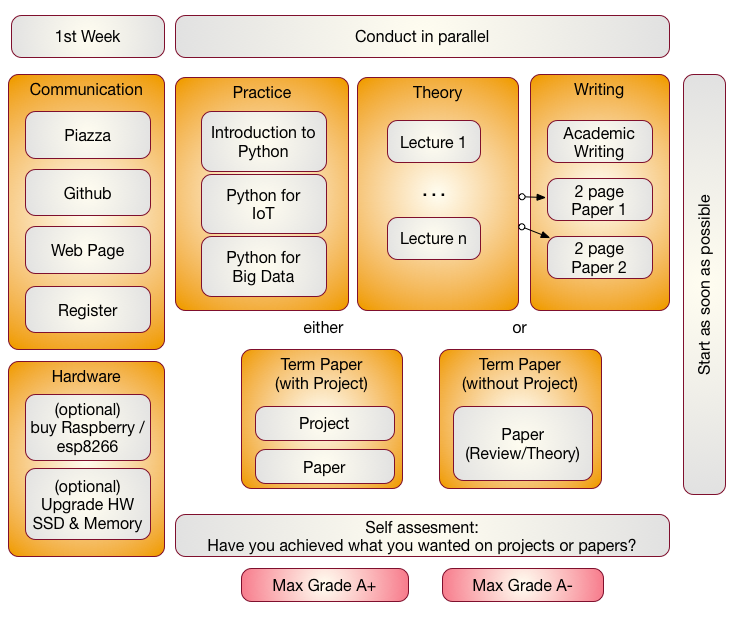
\includegraphics[width=\textwidth]{images/i523-overview.png}
\caption{Components of the Class}
\end{figure}


\subsection{First Week}

In the first week we will be introducing you how we communicate.
Naturally you need to register for the class. Once you register you need
to set up a number of services.

The content for this class will be available through this document
that will be regularly updated. All communication is done with
Piazza. We have prepared a special section on how you can access
Piazza directly from Canvas.

Please follow the instructions and let us know if there are any issues.
You will also need an account on github.com as we like to introduce you
to community tools that are used by the community. Knowing github will
be extremely valuable for you not only for this class, but also once you
graduate. We will have a special lecture for you on this topic and we
expect that you provide us with feedback about your github username.

\subsubsection{Exercise}

\begin{description}
\item[Exercise.Organization.1:] register for the class
\item[Exercise.Organization.2:] obtain a github.com account
\item[Exercise.Organization.3:] enroll in Piazza via Canvas (see
  instructions in the class outline)
\item[Exercise.Organization.4:] create a post in Piazza (use the bio
  folder) (we need to verify you can post). Please use a formal Bio
  and do not use the word ``I''. There are already some examples in
  Piazza that you can follow. Take a look at the bios of the
  instructors.
\item[Exercise.Organization.4:] obtain a chameleon cloud account
\item[Exercise.Organization.5:] obtain a futuresystems.org account
\end{description}

Account creation on FutureSystems and chameleon is only done during
\textbf{working hours} and it may take  a week to get it all worked
out. Do not ask us any questions if the week has not passed.

\subsection{IoT Hardware}

As part of this class you also have the ability to take part in some
Internet of Things related projects and assignments. If you like to
experiment with real hardware, I recommend you to buy an esp8266 or a
Raspberry PI 3. In fact the hardware of both are so cheap that you could
experiment with both of them. Please consult with our hardware page what
is possible. While an esp8266 can be purchased for about \$7 a Raspberry
Pi with case and power supply will cost you about \$50.

\subsection{Access to Clouds}

As part of the course you will also need access to a computer. We will
try best to provide you with access to suitable computers for the class,
but do be reminded that the amount of time and access to supercomputers
and clouds we offer is limited. Our class policy is to use the compute
resources only when you really need them. Thus you \textbf{must} shut
down your VMs when they are not in use. It would be a violation of class
policy if we would find out through an analysis of the cloud logs that
you unnecessarily keep your VMs running. Thus we will implement a
\textbf{strict policy} that you must record yourself how many hours you
run VM's and provide this information to us. We will than compare that
time with the time recorded by the computer system as well as with your
target application and will deduct points form your project if you can
not justify why you have not shut down your VMs. A resource section
needs to be added to your report justifying the used resources.

Why is this such a big deal you may ask? For example we estimate if
every student in class violates this policy it would cost about \$200000
to rent the time for this on a public cloud. Due to this high cost, we
no longer tolerate deliberate violations of the policy and will
terminate your account. Furthermore, violators will have to find
alternative resources to conduct their projects while not using our
resources. In our case the problem is even beyond the issue of cost as
our allocation on the clouds would be terminated due to abuse and
\textbf{no student}, including those that follow policies, could use the
cloud. It may take weeks to reestablish cloud access and would effect
every student in class.

We will provide clarification for accessing cloud resources and teach
you how to avoid getting in such a situation. I am sure that a future
employer of yours will be real happy if you have a deep understanding of
resource vs. cost estimate.

\subsection{Using Your Own Computer}

In many cases however you could be using your own personal computer, but
make sure the computer is up-to-date. This does not mean that you need
to buy a new computer, or need to upgrade it. However, if you consider
an upgrade of an older machine please consider the following.

These days we recommend that your computer has a solid-state drive and
fast maximized memory. Todays home computers have typically 16 GB off
main memory, a minimum of 8GB is required for most operating systems.
Make sure you follow your upgrade guide to your computer and by suitable
memory chips. In most cases you have to buy them in pairs and make sure
all chips in your computer are the same. When it comes to buying a
solid-state drive, make sure that you buy one that is compatible with
motherboards bus speed. As you may want to reuse your solid-state drive
at a later time I suggest to get a 6GB/s SSD and not a 3GB/s.

Students that only had a chromebook and took this class gave us the
feedback that they are too inconvenient as they do not allow you to
program directly in python on them.

If money is an issue, you can buy a Raspberry Pi and edit your programs
there and when satisfied run them on a cloud.

We also like to remind you that this course does not require you to
purchase expensive text books, thus the money you safe on this could be
used in upgrading your hardware or renting yourself from your own money
time on AWS. Hoever, be careful with the cloud its easy to spend lots of
money there if you ar enot careful.

\subsection{Parallel Tracks}

In this class we start out with three parallel tracks. You will be doing
all of them.

\subsubsection{Track 1: Practice}

Trak 1 introduces you to using python for Big Data. Although you do not
need to know any programming language, it is certainly useful as it will
make this course much easier for you. We had students that had no prior
programming knowledge and successfully completed the course. So we know
it can be done. We also had other students that dropped the class as
they felt they need more time to learn programming. It will be up to you
to make that assessment. The course is designed in such a fashion, that
there is enough time to learn programming and do a project.

We provide you with a general introduction to Python. This includes
enough knowledge so you can conduct a project with it. We will reinforce
this knowledge while exposing you to IoT devices that you can program in
Python such as the esp8266 and the Raspberry PI. Residential students
that have purchased a Raspberry PI, will also have the opportunity to
integrate them between each other to create a compute cluster or a
virtual cluster while using state of the art container technology. You
can than compare the compute power of that cluster with your own Laptop,
or a cluster hosted in the cloud.

We will build on these technologies to introduce you to python libraries
that can be used for big data. We also will introduce you to analytics
algorithm such as k-means and others to understand some of their
intrinsic functionality.

Optionally, we also offer you the chance to integrate DevOps into your
projects (which is typically covered in I524) for the most advanced
students of the class. However, we have a real simple solution while
using our own cloudmesh cmd5 to provide an easy interface to
reproducible environments that could be used by anyone in the class.

\subsubsection{Track 2: Theory}

The theory track includes a number of online lectures that introduces
you to a variety of topics related to Big Data. You have especially the
opportunity to become part of a project that would contribute to the
understanding and the development of a Big Data Architecture developed
in collaboration with NIST. Other topics that are covered include IoT,
Health Care, Physics, Science, Biology, Genomics, and so forth. We will
update the Theory track on a weekly basis and will release lectures in
the specified areas. Knowing how to write is a preparation for your term
project/paper.

\subsubsection{Track 3: Writing}

This track will introduce you into how to write an academic paper and
conduct proper bibliography management. Knowing how to write is a
preparation for your term project. If you elect to do a term paper you
still have to conduct the programming assignments.

You will be writing 2 papers that include 2 pages per collaborator on a
particular topic. We like to avoid that all students take the same
topic, so we will identify with you a mechanism to split up the
different topics. We like to conduct the topic assignment ASAP so you
can start. As document format we will be using our class specific 2
column format that can be used either in LaTeX or Word. You can use
collaborative tools such as ShareLatex, Overleaf, and Microsoft
Onedrive. Please not this is an academic paper and not an experience
report, or a magazine article, or a blog. Knowing how to write is a
preparation for your term project/paper.

We noticed a curious observation in previous classes. Other
than one or two exceptions papers written in LaTeX were much better
structured an the content was better than papers written in Word. Thus
LaTeX papers typically received higher grades.

\subsubsection{Track 4: Term Paper/Project}

The major deliverable of the course is a term project or paper. The
exact details will be posted on the Web page and depends on if you
conduct the project/paper in a team or alone. Details will be available,
but will likely replicate what we set for I524. The important part is
that you start on this project once you are sufficiently familiar with
Track 1-3. However you can also use the project to for example learn
python and engage in a goal oriented learning activity while working
towards implementing your project and integrating the python lessons
that you encounter. The same is valid for the theory.

It is \textbf{expected} that you identify a suitable analysis and data
set for the project and that you learn how to apply this analysis as
well as justify it.

More details will be posted once we have introduced you to some
elementary concepts so we can discuss them easier.

Furthermore, it is also important to note that if you do not do a
project (this is your option) the maximum grade for the entire class is
limited to an A-. It will be up to you to assess what you want to do and
self assessment is a real good way to do that. In any case, you should
not expect to get an A if you yourself are not convinced about your
project or are unsure about it. Common sense prevales.

\subsubsection{Self Discipline}

As this class has no graded tests and only few graded homework, we like
that you deliver an \textbf{exceptional} project report or paper.
Instead of focussing on preparing for tests we provide you with the
opportunity to \textbf{explore} without the pressure of grades. However
you should not give up or take the easy way out or it will effect you in
your project execution. Also, to achieve your best do not just say:
\emph{We do not have a test, so let me not do this weeks assignment, let
me do it next week}. After a couple of times with this attitude you will
be in big trouble. All this requires discipline. For example, if you
believe you are so good that you can do a project within one week before
deadline, you will \textbf{certainly fail}. To avoid this and to
introduce discipline, you will also be monitored on progress and we
check your github for activities which will be part of the participation
grade.

\subsubsection{Fun}

I hope you have fun and are able to integrate in the projects your own
thoughts and interrests.

\subsubsection{Uniqueness}

We will try to have every project or paper to be non overlapping with
another topic, If there are overlaps we may ask you to modify your
focus.



\FILENAME

\section{Class Git}\label{class-git}

This class will use git to manage all assignment submissions. We use the
publicly available github.com. The class git is hosted at

\url{https://github.com/orgs/bigdata-i523}

It is in the responsibility of the student to create a github account
and make sure that you will be added to the class github within one week
of joining the class. A TA will be assigned to assist you. Details will
be posted here and an announcement will be made via a piazza post.

\subsection{Exercises}\label{exercises}

\begin{description}
\item[Github.i523.1:]
Create a Github account
\item[Github.i523.2:]
Work with a TA to get added to the github project ((details will be
posted here).
\end{description}


\section{Tutorials, Topic Paper, Term Paper, Project Report}

\FILENAME

Dependendt on the class you need to do different assignments. The
assignments will be clearly posted in this document and updated in
case clarification is needed. 

We use the following terminology:

\begin{description}

\item[Tutorials:] Tutorials are written in markdown, RST, or LaTeX and
  include information on a particular technical issue that is in
  general helpful for other students. Tutorials can be small, but sume
  may need to be substential. As we expect that the tutorials can be
  included in the Handbook, please be careful of plagiarizm and do not
  just copy the tutorial from elswhere. 

\item[Topic Paper:] A topic paper, or short paper is a smapp paper
  about a technology, application, or useful information that provides
  an overview of what you are trying to describe and analyses its
  relatinship to the class topic. Be mindful about plagiarizm. The
  paper is written in \LaTeX and uses jabref for bibliography management. 

\item[Term Paper:] A term paper is an enhanced topic paper. The
  difference is in length. Comparative or review papers can also be
  term papers.  Term papers should have the quality to be publishable
  either in a workshop or as part of the handbook.

\item[Project Paper:] A project reportis an enhanced topic paper that
  includes not just the analysis of a topic, but an actuall code, with
  benchmark or demosntarted appliction use. Obviously it is longer
  than a paper and includes descriptions about reproducability of the
  application. Term papers should have the quality to be publishable
  either in a workshop or as part of the handbook.

\item[Assignments:] In addition to the previously discussed toppict
  you also are doing a small number of assignments. These assignments
  may take you one or multiple weeks to accomplish. Some of them are
  pass fail, while others will receive a grade. It will be clearly
  stated at the beginning of the assignment which of the evaluation
  will apply.

\end{description}

Examples from prior classes are avalable in the class proceedings
listed in Section~\ref{S:p-intro}.

Dependent on the class you have to fulfill different
requirements. Please make sure you understand which requirement you
will have.

\begin{description}

\item[E516] In these classes you will need to produce
  tutorials, topic papers and a project report with real code.

\item[E616] In these classes you will need to produce
  tutorials, topic papers and a project report with real code. 

\item[I524] same as E616, but you have the choice to
  substitute the project report with a term paper.

\end{description}

Please be aware that the project or term paper constitute to a
significant portion of your grade of your class grade. You have plenty
of time to make this choice and if you find you struggle with
programming you may want to consider a term paper instead of a
project.

In case you chose a project your maximum grade for the entire class
could be an A+. However, an A+ project must be truly outstanding and
include an exceptional project report. Such a project and report will
have the potential quality of being able to be published in a
conference.

In case you chose a term Paper for I524 your maximum grade for the
\textit{entire} class will be an A-.

Please note that a project includes writing a project paper.  However
the length is a bit shorter than for a term paper.

\subsection{Team}

Software projects and term papers can be conducted with one, two or
three class members. We do not allow more than three members in a
project, paper, or assignment team. It will be up to you to determine
a team, but we recommend that you chose wisely. Naturally if a team
member does not contribute to the project you need to address this
early on. Please do not come to us a week before the deadline is due
and say a team member has not contributed, this is far to late to do
any adjustment to the team. It is in your responsibility to manage the
team. You can build different teams throughout the semestar for
different tasks. Please communicate clearly and timely with your
class mates.

\subsection{Common Deleiverables}

Both Projects and Term paper have the following common deliverables

\begin{description}
\item[Work Breakdown:]
This is an appendix to the document that describes in detail who did
what in the project. This section comes in a new page after the
references. It does not count towards the page length of the document.
It also includes explicit URLs to the the git history that documents the
statistics to demonstrate not only one student has worked on the
project. If you can not provide such a statistic or all checkins have
been made by a single student, the project has shown that they have not
properly used git. Thus points will be deducted from the project.
Furthermore, if we detect that a student has not contributed to a
project we may invite the student to give a detailed presentation of the
project.
\item[Bibliography:]
All bibliography has to be provided in a jabref/bibtex file. This is
regardless if you use LaTeX or Word. There is \textbf{NO EXCEPTION} to
this rule. PLease be advised doing references right takes some time so
you want to do this early. Please note that exports of Endnote or other
bibliography management tools do not lead to properly formatted bibtex
files, despite they claiming to do so. You will have to clean them up
and we recommend to do it the other way around. Manage your bibliography
with jabref, and if you like to use it import them to endnote or other
tools. Naturally you may have to do some cleanup to. If you use LaTeX
and jabref, you have naturally much less work to do. What you chose is
up to you.
\item[Report Format:]
All reports will be using the our common format. This format is not the
same as the ACM format, so if you use systems such as overleaf or
sharelatex, you need to upload it and use it there.

The format for LaTeX and Word found here:

  \URL{https://github.com/bigdata-i523/sample-hid000/tree/master/paper1}

\end{description}

There will be \textbf{NO EXCEPTION} to this format. In case you are in a
team, you can use either github while collaboratively developing the
LaTeX document or use MicrosoftOne Drive which allows collaborative
editing features. All bibliographical entries must be put into a
bibliography manager such as jabref, endnote, or Mendeley. This will
guarantee that you follow proper citation styles. You can use either ACM
or IEEE reference styles. Your final submission will include the
bibliography file as a separate document.

Documents that do not follow the ACM format and are not accompanied by
references managed with jabref or endnote or are not spell checked will
be returned without review.

\TODO{Integrate the format from the class web page into the LateX
  section More details about the format can be found at
  \url{https://cloudmesh.github.io/classes/lesson/doc/report.html} }

\subsection{Project Paper}

\subsubsection{Systems Usage}

Projects may be executed on your local computer, a cloud or other
resources you may have access to. This may include:

\begin{itemize}
\item chameleoncloud.org
\item furturesystems.org
\item AWS (you will be responsible for charges)
\item Azure (you will be responsible for charges)
\item virtualbox if you have a powerful computer and like to prototype
\item other clouds, please confirm with us.
\end{itemize}

Access to clouds must be scripted and a cmd5 extension must be
developed as part of your project to receive full credit.

\subsubsection{Deliverables}

The following artifacts are part of the deliverables for a project

\begin{description}
\item[Code:]
You must deliver the \textbf{source code} in github. The code must be
compilable and a TA may try to replicate to run your code. You MUST
avoid lengthy install descriptions and everything must be installable
from the command line. We will check submission. All team members must
be responsible for one or all parts of the project.

Code repositories are for code, if you have additional libraries that
are needed you need to develop a script or use a DevOps framework to
install such software. Thus zip files and .class, .o files are not
permissible in the project. Each project must be reproducible with a
simple script. An example is:

\begin{verbatim}
git clone ....
make install
make run
make view
\end{verbatim}

Which would use a simple make file to install, run, and view the
results.  You are expected to integrate cmd5, which we teach in
class. In addition you can use or are expected to us DOCKERFILES,
ansible, or shell scripts. It is not permissible to use GUI based
DevOps preinstalled frameworks. Everything must be installable and
reproducable form the command line.

\item[Data:] Data is to be hosted on IUs google drive if needed. If
  you have larger data, it should be downloaded from the internet. It
  is in your responsibility to develop a download program,
\item[Project Report:] A report must be produced while using the
  format discussed in the Report Format section. The following length
  is required:

\begin{itemize}
\item
  6 pages, one student in the project
\item
  8 pages, two students in the project
\item
  10 pages, three students in the project
\end{itemize}

\item[License:] All projects are developed under an open source
  license such as Apache 2.0 License. You will be required to add a
  LICENCE.txt file and if you use other software identify how it can
  be reused in your project. If your project uses different licenses,
  please add in a README.rst file which packages are used and which
  license these packages have.
\end{description}

\subsection{Term Paper}

In case you chose the term paper, you or your team will pick a topic
relevant for the class. You will write a high quality scholarly paper
about this topic. The following artifacts are part of the deliverables
for a term paper. A report must be produced while using the format
discussed in the Report Format section. The following length is
required:

\begin{itemize}
\item 8 pages, one student in the project
\item 10 pages, two student in the project
\item 12 pages, three student in the project
\end{itemize}


\section{Grading}\label{grading}

Grading for homework will be done within reasonable time of the
submission if the submission was on time. This however could still
take multiple weeks. Students that miss the deadline will be graded on
best effort, which could mean at the end of the semester as TAs will
grade first papers that have been handed in on time.  A 10\% grade
reduction will be given for residential students if the project is
late.  Some homework can not be delivered late (which will be clearly
marked and 0 points will be given if late; these are mostly related to
setting up your account and communicating to us your account names.)

It is the student's responsibility to upload submissions well ahead of
the deadline to avoid last minute problems with network connectivity,
browser crashes, cloud issues, etc. It is a very good idea to make early
submissions and then upload updates as the deadline approaches; we will
grade the last submission received before the deadline.

Note that the term paper or project paper will take a considerable
amount of time and doing proper time management is a must for this
class. Avoid starting your project late. Procrastination does not pay
off. Starting a paper a day or even in the week before the deadline
will allow you not to achieve your best. Late Projects or term papers
will receive a 10\% grade reduction.

For E516 I524, E616 the grading scene is discussed in the syllabus.


\subsection{Grades on Canvas}

The final grade for your class is {\bf NOT} accurately posted in
CANVAS. Please visit the registrar for your final grade.
We have run many times into issues with CANVAS thus we try to stay as
much as possible away form it. We know that the total grade will not
be accurately reported in CANVAS.

Furthermore we are using only a letter grading scheme that
distinguishes qualitatively between grades. Typically we do not engage
in arguing if you get a point more or less. Instead we look at the
artifact and decide if it is an A or A- and so on. CANVAS on the other
hand uses a point system that may provide a misleading information as
we do not use points.

Once the due date is passed all incomplete assignments will appear as
an \textit{F} in CANVAS. Once we receive and review the submission this grade will
be changed. Please, do not cintact us if you submitted late and you
see an F in CANVAS temportrarily.

\subsection{Discussion about Grades}

Should it be necessary a discussion about a grade must not be taking
place via e-mail nor via piazza. YOu must use the CANVAS message
feature as we want to make sure that by accident you post information
to others that you do not intend to. FOr this reason we will not read
such messages on pizza and in our e-mail and deleted them without reading.



\chapter{Assignments}\label{c:222-assignments}

\section{Assignments E222}
\label{s:e222-assignment}
\label{s:e222-assignments}
\index{Assignments!E222}

\subsection{Bio Post}
\label{E:e222-bio}

\begin{exercise}\label{E:e222-bio-piazza}
{\bf Bio Post on Piazza.} Please post a formal bio to piazza
\end{exercise}

\begin{exercise} \label{E:e222-bio-googledocs}

  {\bf Bio Post in Google doc.} After you have posted it to piazza
  copy your updated formal bios into the following document.  Make
  sure you use 3rd person and stay formal. This is a formal
  bio. Comment on the effectiveness of using the cloud service for
  this task. A the end of the document. This assignment does not
  replace the post of the bio to piazza, it is used to gather all bios
  in one document and to evaluate if google docs is a good tool for
  this kind of task. Remember we have lots of students and google is
  used often just with small groups.
 
 \smallskip

 {\hfill \href{https://docs.google.com/document/d/1ejzlKYqC3dLac8WXVpcPQsJh1j4BDqRxxgGg1cFQbeQ/edit?usp=sharing}{E222 Link to google doc $\mapsto$}}

 \end{exercise}

\subsection{IU Google Services}
\label{E:e222-iu-google-services}

\begin{exercise}\label{E:e222-iu-google}

  {\bf IU Google Services:} This assignment is only for those that do
  not yet have access to our google documents This assignment does not
  have to be conducted for anyone that has access to our google
  documents for bios, and the technology list

  \begin{itemize}
 
  \item What is the difference between umail.iu.edu and iu.edu? Tip:
    the answer is provided in the IU knowledge base

  \item Login via the iu.edu account and not the umail.iu.edu account
    to google and open the document for the bio. Paste the bio into
    the document.

  \item Explain why IU has two different google services and
    logins. As we use cloud in this class, it is important to
    understand this and what implication this has. This is not just an
    assignment to give you access to the service, but to make you
    think why this works like this.

  \item Can you imagine a different way this ought to work?

  \end{itemize}

\end{exercise}

\section{Assignments E516, I524, E616}
\label{s:616-assignments}
\index{Assignments!E516}
\index{Assignments!E616}
\index{Assignments!I524}

\subsection{Bio Post}\label{a:616-bio}

\begin{exercise}\label{E:616-bio-piazza}
{\bf Bio Post on Piazza.} Please post a formal bio to piazza
\end{exercise}

\begin{exercise} \label{E:616-bio-googledocs}

  {\bf Bio Post in Google doc.} After you have posted it to piazza
  copy your updated formal bios into the following document.  Make
  sure you use 3rd person and stay formal. This is a formal
  bio. Comment on the effectiveness of using the cloud service for
  this task. A the end of the document. This assignment does not
  replace the post of the bio to piazza, it is used to gather all bios
  in one document and to evaluate if google docs is a good tool for
  this kind of task. Remember we have lots of students and google is
  used often just with small groups.
 
 \smallskip

 {\hfill \href{https://docs.google.com/document/d/1ejzlKYqC3dLac8WXVpcPQsJh1j4BDqRxxgGg1cFQbeQ/edit?usp=sharing}{E516 Link to google doc $\mapsto$}}

 \end{exercise}

\subsection{IU Google Services}
\label{E:e616-iu-google-services}

\begin{exercise}\label{E:616-iu-google}

  {\bf IU Google Services:} This assignment is only for those that do
  not yet have access to our google documents This assignment does not
  have to be conducted for anyone that has access to our google
  documents for bios, and the technology list

  \begin{itemize}
 
  \item What is the difference between umail.iu.edu and iu.edu? Tip:
    the answer is provided in the IU knowledge base

  \item Login via the iu.edu account and not the umail.iu.edu account
    to google and open the document for the bio. Paste the bio into
    the document.

  \item Explain why IU has two different google services and
    logins. As we use cloud in this class, it is important to
    understand this and what implication this has. This is not just an
    assignment to give you access to the service, but to make you
    think why this works like this.

  \item Can you imagine a different way this ought to work?

  \end{itemize}

\end{exercise}


\subsection{Big Data Collaboration}
\label{E:616-bigdata-collab}

\begin{exercise} \label{E:616-big-data-and-collaboration} {\bf Big
    data and collaboration.}The purpose of this assignment is
  multifold; test the ability of Google docs to be used in
  collaborative fashion by more than a small group and report on the
  experience. Good Things and bad things, learn on how to use Google
  docs with headings and table of contents learn how to gather
  resources quickly with hyperlinks to web resources or articles and
  translate them into formal academic references. Most importantly
  convey some very important feature of big data.Contribute this into
  the handbook for everyone's benefit (done by TAs).  \smallskip

  \noindent {\bf Task:} Your task is to identify Big Data size related
  articles and Web resources and produce a historical development of
  the growth of this data

  {\hfill \href{https://docs.google.com/document/d/1ZHNdhX_Jx7uBQo0kthSYQ6TQR8_KNbgOwH2EuqBQcjY/edit?usp=sharing}{E516 Link to google doc $\mapsto$}}



\end{exercise}



\subsection{New Technology List}
\label{E:616-new-tech}

\begin{exercise} 
Due: Jan 29

The handbook contains a large number of technologies to which an
abstract is provided.

Your task is to identify FIRST not to do an abstract but to
collaboratively gather a LIST of new technologies that are important
in Cloud and Big Data. We suggest doing this in a google docs document
first. Write Lastname, Firstname, class id behind the technology so we
know who contributed it. Indicate also if commercial, or open source,
We are mostly interested in open source activities. Keep the list
sorted by alphabet. Use a bullet so formatting is preserved

\url{https://docs.google.com/document/d/1LeHGHTSBbaPXYVor0efhmi5W7JJjS7EQHABHqgRAPuU/edit?usp=sharing}

Example: 

OpenWhisk, \url{https://openwhisk.apache.org/}, open source, Gregor von Laszewski, e616

\end{exercise}


\subsection{New Technology Abstract}
\label{E:616-new-tech-abstract}

\begin{exercise} 
 
Due date: Feb 5th

We have gathered with the technology list 

\url{https://piazza.com/class/jbkvbp3ed3m2ez?cid=50}

a number of technologies that are not yet covered in the handbook or
need improvement in the handbook.

The TAs will be selecting about 5 technologies for each student. Each
student will write high-quality non-plagiarized abstracts which bibtex
references.
 
Learning outcomes:

\begin{itemize}

\item Identify how to not plagiarize
\item Work in a large team (with coordination by TAs)
\item Use bibtex and jabref for reference management which you will be using for your final paper
\item Find new trends in big data and cloud computing

\end{itemize}

\end{exercise}












%----------------------------------------------------------------------------------------
%	PART
%----------------------------------------------------------------------------------------

\part{Python}

%----------------------------------------------------------------------------------------
%	CHAPTER 1
%----------------------------------------------------------------------------------------

\chapterimage{chapter_head_2.png} % Chapter heading image

\chapter{Introduction}

\begin{fileremark}\url{https://github.com/cloudmesh/classes/blob/master/docs/source/lesson/prg/python-intro.rst}\end{fileremark}
\section{Introduction to Python}\label{introduction-to-python}

Portions of this lesson have been adapted from the
\href{https://docs.python.org/2/tutorial/}{official Python Tutorial}
copyright \href{http://www.python.org/}{Python Software Foundation}.

Python is an easy to learn programming language. It has efficient
high-level data structures and a simple but effective approach to
object-oriented programming. Python's simple syntax and dynamic typing,
together with its interpreted nature, make it an ideal language for
scripting and rapid application development in many areas on most
platforms. The Python interpreter and the extensive standard library are
freely available in source or binary form for all major platforms from
the Python Web site, \url{https://www.python.org/}, and may be freely
distributed. The same site also contains distributions of and pointers
to many free third party Python modules, programs and tools, and
additional documentation. The Python interpreter can be extended with
new functions and data types implemented in C or C++ (or other languages
callable from C). Python is also suitable as an extension language for
customizable applications.

Python is an interpreted, dynamic, high-level programming language
suitable for a wide range of applications.

The philosophy of python is summarized in
\href{https://www.python.org/dev/peps/pep-0020/}{The Zen of Python} as
follows:

\begin{itemize}
\tightlist
\item
  Explicit is better than implicit
\item
  Simple is better than complex
\item
  Complex is better than complicated
\item
  Readability counts
\end{itemize}

The main features of Python are:

\begin{itemize}
\tightlist
\item
  Use of indentation whitespace to indicate blocks
\item
  Object orient paradigm
\item
  Dynamic typing
\item
  Interpreted runtime
\item
  Garbage collected memory management
\item
  a large standard library
\item
  a large repository of third-party libraries
\end{itemize}

Python is used by many companies (such as Google, Yahoo!, CERN, NASA)
and is applied for web development, scientific computing, embedded
applications, artificial intelligence, software development, and
information security, to name a few.

\subsection{About the Tutorial}\label{about-the-tutorial}

This tutorial introduces the reader informally to the basic concepts and
features of the Python language and system. It helps to have a Python
interpreter handy for hands-on experience, but all examples are
self-contained, so the tutorial can be read off-line as well. At the end
of this lesson you will be able to:

\begin{itemize}
\tightlist
\item
  use Python
\item
  use the interactive Python interface
\item
  understand the basic syntax of Python
\item
  write and run Python programs stored in a file
\item
  have an overview of the standard library
\item
  install Python libraries using pyenv or if it is not available
  virtualenv
\end{itemize}

This tutorial does not attempt to be comprehensive and cover every
single feature, or even every commonly used feature. Instead, it
introduces many of Python's most noteworthy features, and will give you
a good idea of the language's flavor and style. After reading it, you
will be able to read and write Python modules and programs, and you will
be ready to learn more about the various Python library modules.

In order to conduct this lesson you need

\begin{itemize}
\tightlist
\item
  A computer with Python 2.7.13 or 3.6.2
\item
  Familiarity with command line usage
\item
  A text editor such as
  \href{https://www.jetbrains.com/pycharm/}{PyCharm}, emacs, vi or
  others. You should identity which works best for you and set it up.
\end{itemize}

\subsection{Links}\label{links}

\begin{itemize}
\tightlist
\item
  \href{https://www.python.org/}{Python}
\item
  \href{https://pip.pypa.io/en/stable/}{Pip}
\item
  \href{https://virtualenv.pypa.io/en/stable/}{Virtualenv}
\item
  \href{http://www.numpy.org/}{NumPy}
\item
  \href{https://scipy.org/}{SciPy}
\item
  \href{http://matplotlib.org/}{Matplotlib}
\item
  \href{http://pandas.pydata.org/}{Pandas}
\item
  \href{https://github.com/pyenv/pyenv}{pyenv}
\item
  \href{https://github.com/pyenv/pyenv}{PyCharm}
\end{itemize}

Python module of the week is a Web site that provides a number of short
examples on how to use some elementary python modules. Not all modules
are equally useful and you should decide if there are better
alternatives. However for beginners this site provides a number of good
examples

\begin{itemize}
\tightlist
\item
  Python 2: \url{https://pymotw.com/2/}
\item
  Python 3: \url{https://pymotw.com/3/}
\end{itemize}


\chapter{Install}

\begin{fileremark}\url{https://github.com/cloudmesh/classes/blob/master/docs/source/lesson/prg/python-install.rst}\end{fileremark}
\section{Python Installation}\label{python-installation}

Python is easy to install and very good instructions for most platforms
can be found on the python.org Web page. We will be using Python 2.7.13
and/or Python 3 in our activities.

To manage python modules, it is useful to have
\href{https://pypi.python.org/pypi/pip}{pip} package installation tool
on your system.

In the tutorial, we assume that you have a computer with python
installed. However, we also recommend that for the class you use
Python's virtualenv (see below) to isolate your development Python from
the system installed Python.

\subsection{Managing custom Python
installs}\label{managing-custom-python-installs}

Often you have your own computer and you do not like to change its
environment to keep it in pristine condition. Python comes with mnay
libraries that could for example conflict with libraries that you have
installed. To avoid this it is bets to work in an isolated python we can
use tools such as virtualenv, pyenv or pyvenv for 3.6.2. Which you use
depends on you, but we highly recommend pyenv if you can.

\subsubsection{Managing Multiple Python Versions with
Pyenv}\label{managing-multiple-python-versions-with-pyenv}

Python has several versions that are used by the community. This
includes Python 2 and Python 3, but alls different management of the
python libraries. As each OS may have their own version of python
installed. It is not recommended that you modify that version. Instead
you may want to create a localized python installation that you as a
user can modify. To do that we recommend \emph{pyenv}. Pyenv allows
users to switch between multiple versions of Python
(\url{https://github.com/yyuu/pyenv}). To summarize:

\begin{itemize}
\tightlist
\item
  users to change the global Python version on a per-user basis;
\item
  users to enable support for per-project Python versions;
\item
  easy version changes without complex environment variable management;
\item
  to search installed commands across different python versions;
\item
  integrate with tox (\url{https://tox.readthedocs.io/}).
\end{itemize}

\paragraph{Instalation without pyenv}\label{instalation-without-pyenv}

If you need to have more than one python version installed and do not
want or can use pyenv, we recommend you download and install python
2.7.13 and 3.6.2 from python.org
(\url{https://www.python.org/downloads/})

\paragraph{Disabeling wrong python installs on
OSX}\label{disabeling-wrong-python-installs-on-osx}

While working with students we have seen at times that they take other
classes either at universities or online that teach them how to program
in python. Unfortuanatley, although they seem to do that they often
ignore to teach you how to properly install python. I just reachentl had
a students that had installed python 7 times on his OSX machine, while
another student had 3 different instalations, all of which confliced
with each other as they were not set up properly.

We recommend that you inspect if you have a files such as
\textasciitilde{}/.bashrc or \textasciitilde{}/.bashrc\_profile in your
ehome directory and identify if it activates various versions of python
on your computer. If so you could try to deactivate them while
outcommenting the various versions with the \# character at the
beginning of the line, start a new terminal and see if the terminal
shell still works. Than you can follow our instructions here while using
an install on pyenv.

\paragraph{Install pyenv on OSX from
git}\label{install-pyenv-on-osx-from-git}

This is our recommended way to install pyenv on OSX:

\begin{verbatim}
$ git clone https://github.com/pyenv/pyenv.git ~/.pyenv
$ git clone https://github.com/pyenv/pyenv-virtualenv.git ~/.pyenv/plugins/pyenv-virtualenv
$ git clone https://github.com/yyuu/pyenv-virtualenvwrapper.git ~/.pyenv/plugins/pyenv-virtualenvwrapper
$ echo 'export PYENV_ROOT="$HOME/.pyenv"' >> ~/.bash_profile
$ echo 'export PATH="$PYENV_ROOT/bin:$PATH"' >> ~/.bash_profile
\end{verbatim}

\paragraph{Instalation of Homebrew}\label{instalation-of-homebrew}

Before installing anything on your computer make sure you have enough
space. Use in the terminal the command:

\begin{verbatim}
$ df -h
\end{verbatim}

which gives your an overview of your file system. If you do not have
enough space, please make sure you free up unused files from your drive.

In many occasions it is beneficial to use readline as it provides nice
editing features for the terminal and xz for completion. First, make
sure you have xcode installed:

\begin{verbatim}
$ xcode-select --install
\end{verbatim}

Next install homebrew, pyenv, pyenv-virtualenv and pyenv-virtualwrapper.
Additionally install readline and some compression tools:

\begin{verbatim}
/usr/bin/ruby -e "$(curl -fsSL https://raw.githubusercontent.com/Homebrew/install/master/install)"
brew update
brew install readline xz
\end{verbatim}

\paragraph{Install pyenv on OSX with
Homebrew}\label{install-pyenv-on-osx-with-homebrew}

We describe here a mechanism of installing pyenv with homebrew. Other
mechanisms can be found on the pyenv documentation page
(\url{https://github.com/yyuu/pyenv-installer}). You must have homebrew
installed as discussed in the previous section.

To install pyenv with homebrew execute in the terminal:

\begin{verbatim}
brew install pyenv pyenv-virtualenv pyenv-virtualenvwrapper
\end{verbatim}

\paragraph{Install pyenv on Ubuntu}\label{install-pyenv-on-ubuntu}

The following steps will install pyenv in a new ubuntu 16.04
distribution.

Start up a terminal and execute in the terminal the following commands.
We recommend that you do it one command at a time so you can observe if
the command succeeds:

\begin{verbatim}
$ sudo apt-get update
$ sudo apt-get install git python-pip make build-essential libssl-dev
$ sudo apt-get install zlib1g-dev libbz2-dev libreadline-dev libsqlite3-dev
$ sudo pip install virtualenvwrapper

$ git clone https://github.com/yyuu/pyenv.git ~/.pyenv
$ git clone https://github.com/pyenv/pyenv-virtualenv.git ~/.pyenv/plugins/pyenv-virtualenv   
$ git clone https://github.com/yyuu/pyenv-virtualenvwrapper.git ~/.pyenv/plugins/pyenv-virtualenvwrapper

$ echo 'export PYENV_ROOT="$HOME/.pyenv"' >> ~/.bashrc
$ echo 'export PATH="$PYENV_ROOT/bin:$PATH"' >> ~/.bashrc
\end{verbatim}

Now that you have installed pyenv it is not yet activated in your
current terminal. The easiest thing to do is to start a new terminal and
typ in:

\begin{verbatim}
which pyenv
\end{verbatim}

If you see a response pyenv is installed and you can proceed with the
next steps.

\begin{description}
\item[Please remember whenever you modify .bashrc or]
.bash\_profile you need to start a new terminal.
\end{description}

\paragraph{Install Different Python
Versions}\label{install-different-python-versions}

Pyenv provides a large list of different python versions. To see the
entire list please use the command:

\begin{verbatim}
$ pyenv install -l
\end{verbatim}

However, for us we only need to worry about python 2.7.13 and python
3.6.2 (once 3.6.2 becomes available we will use that). You can now
install different versions of python into your local environment with
the following commands:

\begin{verbatim}
$ pyenv install 2.7.13
$ pyenv install 3.6.2
\end{verbatim}

You can set the global python default version with:

\begin{verbatim}
$ pyenv global 2.7.13
\end{verbatim}

Type the following to determine which version you activated:

\begin{verbatim}
$ pyenv version
\end{verbatim}

Type the following to determine which versions you have available:

\begin{verbatim}
$ pyenv versions
\end{verbatim}

Associate a specific environment name with a certain python version, use
the following commands:

\begin{verbatim}
$ pyenv virtualenv 2.7.13 ENV2
$ pyenv virtualenv 3.6.2 ENV3
\end{verbatim}

In the example above, ENV2 would represent python 2.7.13 while ENV3
would represent python 3.6.2. Often it is easier to type the alias
rather than the explicit version.

\paragraph{Set up the Shell}\label{set-up-the-shell}

To make all work smoothly from your terminal, you can include the
following in your .bashrc files:

\begin{verbatim}
export PYENV_VIRTUALENV_DISABLE_PROMPT=1
eval "$(pyenv init -)"
eval "$(pyenv virtualenv-init -)"

__pyenv_version_ps1() {
  local ret=$?;
  output=$(pyenv version-name)
  if [[ ! -z $output ]]; then
    echo -n "($output)"
  fi
  return $ret;
}

PS1="\$(__pyenv_version_ps1) ${PS1}"
\end{verbatim}

We recommend that you do this towards the end of your file.

\paragraph{Switching Environments}\label{switching-environments}

After setting up the different environments, switching between them is
now easy. Simply use the following commands:

\begin{verbatim}
(2.7.13) $ pyenv activate ENV2
(ENV2) $ pyenv activate ENV3
(ENV3) $ pyenv activate ENV2
(ENV2) $ pyenv deactivate ENV2
(2.7.13) $ 
\end{verbatim}

To make it even easier, you can add the following lines to your
.bash\_profile file:

\begin{verbatim}
alias ENV2="pyenv activate ENV2"
alias ENV3="pyenv activate ENV3"
\end{verbatim}

If you start a new terminal, you can switch between the different
versions of python simply by typing:

\begin{verbatim}
$ ENV2
$ ENV3
\end{verbatim}

\subsection{Instalation without
pyenv}\label{instalation-without-pyenv-1}

If you need to have more than one python version installed and do not
want or can use pyenv, we recommend you download and install python
2.7.13 and 3.6.2 from python.org
(\url{https://www.python.org/downloads/})

\subsubsection{Make sure pip is up to
date}\label{make-sure-pip-is-up-to-date}

As you will want to install other packages, make sure pip is up to date:

\begin{verbatim}
pip install pip -U
\end{verbatim}

pyenv virtualenv anaconda3-4.3.1 ANA3 pyenv activate ANA3

\subsection{Anaconda and Miniconda}\label{anaconda-and-miniconda}

\begin{description}
\item[We do not recommend that you use anaconda or miniconda as it may]
interfere with your default python interpreters and setup.
\end{description}

Please note that beginners to pyton should always use anaconda or
miniconda only afterthey have installed pyenv and use it. For this class
neither anaconda nor miniconda is required. In fact we do not recommend
it. We keep this section as we know that other classes at IU may use
anaconda. We are not aware if these classes teach you the right way to
install it, with \emph{pyenv}.

\subsubsection{Miniconda}\label{miniconda}

\begin{description}
\item[This section about miniconda is experimental and has not]
been tested. We are looking for contributors that help completing it. If
you use anaconda or miniconda we recommend to manage it via pyenv.
\end{description}

To install mini conda you can use the following commands:

\begin{verbatim}
$ mkdir ana
$ cd ana
$ pyenv install miniconda3-latest
$ pyenv local miniconda3-latest
$ pyenv activate miniconda3-latest
$ conda create -n ana anaconda
\end{verbatim}

To activate use:

\begin{verbatim}
$ source activate ana
\end{verbatim}

To deactivate use:

\begin{verbatim}
$ source deactivate
\end{verbatim}

To install cloudmesh cmd5 please use:

\begin{verbatim}
$ pip install cloudmesh.cmd5
$ pip install cloudmesh.sys
\end{verbatim}

\subsubsection{Anaconda}\label{anaconda}

\begin{description}
\item[This section about anaconda is experimental and has not]
been tested. We are looking for contributors that help completing it.
\end{description}

You can add anaconda to your pyenv with the following commands:

\begin{verbatim}
pyenv install anaconda3-4.3.1
\end{verbatim}

To switch more easily we recommend that you use the following in your
.bash\_profile file:

\begin{verbatim}
alias ANA="pyenv activate anaconda3-4.3.1"
\end{verbatim}

Once you have done this you can easily switch to anaconda with the
command:

\begin{verbatim}
$ ANA
\end{verbatim}

Terminology in annaconda could lead to confusion. Thus we like to point
out that the version number of anaconda is unrelated to the python
version. Furthermore, anaconda uses the term root not for the root user,
but for the originating directory in which the anaconda program is
installed.

In case you like to build your own conda packages at a later time we
recommend that you install the conda-build package:

\begin{verbatim}
$ conda install conda-build
\end{verbatim}

When executing:

\begin{verbatim}
pyenv versions
\end{verbatim}

you will see after the install completed the anaconda versions
installed:

\begin{verbatim}
pyenv versions
system
2.7.13
2.7.13/envs/ENV2
3.6.2
3.6.2/envs/ENV3
ENV2 
ENV3
* anaconda3-4.3.1 (set by PYENV_VERSION environment variable)
\end{verbatim}

Let us now create virtualenv for anaconda:

\begin{verbatim}
$ pyenv virtualenv anaconda3-4.3.1 ANA
\end{verbatim}

To activate it you can now use:

\begin{verbatim}
$ pyenv ANA
\end{verbatim}

However, anaconda may modify your .bashrc or .bash\_profile files and ,
may result in incompatibilities with other python versions. For this
reason we recommend not to use it. If you find ways to get it to work
reliably with other versions, please let us know and we update this
tutorial.

To install cloudmesh cmd5 please use:

\begin{verbatim}
$ pip install cloudmesh.cmd5
$ pip install cloudmesh.sys
\end{verbatim}

\paragraph{Exercise}\label{exercise}

\begin{description}
\item[Epyenv.1:]
Write installation instructions for an operating system of your choice
and add to this documentation.
\item[Epyenv.2:]
Replicate the steps above, so you can type in ENV2 and ENV3 in your
terminals to switch between python 2 and 3.
\end{description}

\subsubsection{virtualenv}\label{virtualenv}

environment while using virtualenv,. Documentation about it can be found
at:

\begin{verbatim}
* https://virtualenv.pypa.io
\end{verbatim}

The installation is simple once you have pip installed. If it is not
installed you can say:

\begin{verbatim}
$ easy_install pip
\end{verbatim}

After that you can install the virtual env with:

\begin{verbatim}
$ pip install virtualenv
\end{verbatim}

To setup an isolated environment for example in the directory
\textasciitilde{}/ENV please use:

\begin{verbatim}
$ virtualenv ~/ENV
\end{verbatim}

To activate it you can use the command:

\begin{verbatim}
$ source ~/ENV/bin/activate
\end{verbatim}

you can put this command in your .bashrc or .bash\_profile files so you
do not forget to activate it. Instructions for this can be
found in our lesson on Linux \textless{}bashrc\textgreater{}.


\chapter{Language}

\begin{fileremark}\url{https://github.com/cloudmesh/classes/blob/master/docs/source/lesson/prg/python.rst}\end{fileremark}
\section{Interactive Python}\label{interactive-python}

Python can be used interactively. Start by entering the interactive loop
by executing the command:

\begin{verbatim}
$ python
\end{verbatim}

You should see something like the following:

\begin{verbatim}
Python 2.7.13 (default, Nov 19 2016, 06:48:10)
[GCC 5.4.0 20160609] on linux2
Type "help", "copyright", "credits" or "license" for more information.
>>>
\end{verbatim}

The \textgreater{}\textgreater{}\textgreater{} is the prompt for the
interpreter. This is similar to the shell interpreter you have been
using.

Often we show the prompt when illustrating an example. This is to
provide some context for what we are doing. If you are following along
you will not need to type in the prompt.

This interactive prompt does the following:

\begin{itemize}
\tightlist
\item
  \emph{read} your input commands
\item
  \emph{evaluate} your command
\item
  \emph{print} the result of evaluation
\item
  \emph{loop} back to the beginning.
\end{itemize}

This is why you may see the interactive loop referred to as a
\textbf{REPL}:
\textbf{R}ead-\textbf{E}valuate-\textbf{P}rint-\textbf{L}oop.

\section{Python 3 Features in Python
2}\label{python-3-features-in-python-2}

As mentioned earlier, we assume you will use Python 2.7.X because there
are still some libraries that haven't been ported to Python 3. However,
there are some features of Python 3 we can and want to use in Python
2.7. Before we do anything else, we need to make these features
available to any subsequent code we write:

\begin{verbatim}
>>> from __future__ import print_function, division
\end{verbatim}

The first of these imports allows us to use the print function to output
text to the screen, instead of the print statement, which Python 2 uses.
This is simply a \href{https://www.python.org/dev/peps/pep-3105/}{design
decision} that better reflects Python's underlying philosophy.

The second of these imports makes sure that the
\href{https://www.python.org/dev/peps/pep-0238/}{division operator}
behaves in a way a newcomer to the language might find more intruitive.
In Python 2, division / is \emph{floor division} when the arguments are
integers, meaning that 5 / 2 == 2, for example. In Python 3, division /
is \emph{true division}, thus 5 / 2 == 2.5.

\section{Statements and Strings}\label{statements-and-strings}

Let us explore the syntax of Python. Type into the interactive loop and
press Enter:

\begin{verbatim}
>>> print("Hello world from Python!")
Hello world from Python!
\end{verbatim}

What happened: the print function was given a \textbf{string} to
process. A string is a sequence of characters. A \textbf{character} can
be a alphabetic (A through Z, lower and upper case), numeric (any of the
digits), white space (spaces, tabs, newlines, etc), syntactic directives
(comma, colon, quotation, exclamation, etc), and so forth. A string is
just a sequence of the character and typically indicated by surrounding
the characters in double quotes.

Standard output is discussed in the ../../lesson/linux/shell lesson.

So, what happened when you pressed Enter? The interactive Python program
read the line print "Hello world from Python!", split it into the print
statement and the "Hello world from Python!" string, and then executed
the line, showing you the output.

\section{Variables}\label{variables}

You can store data into a \textbf{variable} to access it later. For
instance, instead of:

\begin{verbatim}
>>> print('Hello world from Python!')
\end{verbatim}

which is a lot to type if you need to do it multiple times, you can
store the string in a variable for convenient access:

\begin{verbatim}
>>> hello = 'Hello world from Python!'
>>> print(hello)
Hello world from Python!
\end{verbatim}

\section{Data Types}\label{data-types}

\subsection{Booleans}\label{booleans}

A \textbf{boolean} is a value that indicates \emph{truthness} of
something. You can think of it as a toggle: either ``on'' or ``off'',
``one'' or ``zero'', ``true'' or ``false''. In fact, the only possible
values of the \textbf{boolean} (or bool) type in Python are:

\begin{itemize}
\tightlist
\item
  True
\item
  False
\end{itemize}

You can combine booleans with \textbf{boolean operators}:

\begin{itemize}
\tightlist
\item
  and
\item
  or
\end{itemize}

\begin{verbatim}
>>> print(True and True)
True
>>> print(True and False)
False
>>> print(False and False)
False
>>> print(True or True)
True
>>> print(True or False)
True
>>> print(False or False)
False
\end{verbatim}

\subsection{Numbers}\label{numbers}

The interactive interpreter can also be used as a calculator. For
instance, say we wanted to compute a multiple of 21:

\begin{verbatim}
>>> print(21 * 2)
42
\end{verbatim}

We saw here the print statement again. We passed in the result of the
operation 21 * 2. An \textbf{integer} (or \textbf{int}) in Python is a
numeric value without a fractional component (those are called
\textbf{floating point} numbers, or \textbf{float} for short).

The mathematical operators compute the related mathematical operation to
the provided numbers. Some operators are:

\begin{itemize}
\tightlist
\item
  * --- multiplication
\item
  / --- division
\item
  + --- addition
\item
  - --- subtraction
\item
  ** --- exponent
\end{itemize}

Exponentiation is read as x**y is x to the yth power:

\[x^y\]

You can combine \textbf{float}s and \textbf{int}s:

\begin{verbatim}
>>> print(3.14 * 42 / 11 + 4 - 2)
13.9890909091
>>> print(2**3)
8
\end{verbatim}

Note that \textbf{operator precedence} is important. Using parenthesis
to indicate affect the order of operations gives a difference results,
as expected:

\begin{verbatim}
>>> print(3.14 * (42 / 11) + 4 - 2)
11.42
>>> print(1 + 2 * 3 - 4 / 5.0)
6.2
>>> print( (1 + 2) * (3 - 4) / 5.0 )
-0.6
\end{verbatim}

\section{REPL (Read Eval Print Loop)}\label{repl-read-eval-print-loop}

We have so far seen a few examples of types: \textbf{string}s,
\textbf{bool}s, \textbf{int}s, and \textbf{float}s. A \textbf{type}
indicates that values of that type support a certain set of operations.
For instance, how would you exponentiate a string? If you ask the
interpreter, this results in an error:

\begin{verbatim}
>>> "hello"**3
Traceback (most recent call last):
  File "<stdin>", line 1, in <module>
TypeError: unsupported operand type(s) for ** or pow(): 'str' and 'int'
\end{verbatim}

There are many different types beyond what we have seen so far, such as
\textbf{dictionaries}s, \textbf{list}s, \textbf{set}s. One handy way of
using the interactive python is to get the type of a value using
`type():

::

   \textgreater{}\textgreater{}\textgreater{} type(42)
   \textless{}type 'int'\textgreater{}
   \textgreater{}\textgreater{}\textgreater{} type(hello)
   \textless{}type 'str'\textgreater{}
   \textgreater{}\textgreater{}\textgreater{} type(3.14)
   \textless{}type 'float'\textgreater{}

You can also ask for help about something using help():

::

   \textgreater{}\textgreater{}\textgreater{} help(int)
   \textgreater{}\textgreater{}\textgreater{} help(list)
   \textgreater{}\textgreater{}\textgreater{} help(str)

.. tip::

   Using help()` opens up a pager. To navigate you can use the spacebar
to go down a page w to go up a page, the arrow keys to go up/down
line-by-line, or q to exit.

\section{Module Management}\label{module-management}

A module allows you to logically organize your Python code. Grouping
related code into a module makes the code easier to understand and use.
A module is a Python object with arbitrarily named attributes that you
can bind and reference. A module is a file consisting of Python code. A
module can define functions, classes and variables. A module can also
include runnable code.

\subsection{Import Statement}\label{import-statement}

\begin{quote}
When the interpreter encounters an import statement, it imports the
module if the module is present in the search path. A search path is a
list of directories that the interpreter searches before importing a
module. The from\ldots{}import Statement Python's from statement lets
you import specific attributes from a module into the current namespace.
The from\ldots{}import has the following syntax − from modname:
\end{quote}

import name1{[}, name2{[}, \ldots{} nameN{]}{]}

When the interpreter encounters an import statement, it imports the
module if the module is present in the search path. A search path is a
list of directories that the interpreter searches before importing a
module.

\subsection{The from \ldots{} import
Statement}\label{the-from-import-statement}

Python's from statement lets you import specific attributes from a
module into the current namespace. The from \ldots{} import has the
following syntax:

\begin{verbatim}
::
\end{verbatim}

\begin{quote}
from module1 import name1{[}, name2{[}, \ldots{} nameN{]}{]}
\end{quote}

\section{Date Time in Python}\label{date-time-in-python}

The datetime module supplies classes for manipulating dates and times in
both simple and complex ways. While date and time arithmetic is
supported, the focus of the implementation is on efficient attribute
extraction for output formatting and manipulation. For related
functionality, see also the time and calendar modules.

The import Statement You can use any Python source file as a module by
executing an import statement in some other Python source file.

\begin{verbatim}
>>>from datetime import datetime
\end{verbatim}

This module offers a generic date/time string parser which is able to
parse most known formats to represent a date and/or time.

\begin{verbatim}
>>>from dateutil.parser import parse
\end{verbatim}

pandas is an open source Python library for data analysis that needs to
be imported.

\begin{verbatim}
>>>import pandas as pd
\end{verbatim}

Create a string variable with the class start time

\begin{verbatim}
>>>fall_start = '08-21-2017'
\end{verbatim}

Convert the string to datetime format

\begin{verbatim}
>>>datetime.strptime(fall_start, '%m-%d-%Y')
datetime.datetime(2017, 8, 21, 0, 0)
\end{verbatim}

Creating a list of strings as dates

\begin{verbatim}
>>>class_dates = ['8/25/2017', '9/1/2017', '9/8/2017', '9/15/2017', '9/22/2017', '9/29/2017']
\end{verbatim}

Convert Class\_dates strings into datetime format and save the list into
variable a

\begin{verbatim}
>>>a = [datetime.strptime(x, '%m/%d/%Y') for x in class_dates]
\end{verbatim}

Use parse() to attempt to auto-convert common string formats. Parser
must be a string or character stream, not list.

\begin{verbatim}
>>>parse(fall_start)
datetime.datetime(2017, 8, 21, 0, 0)
\end{verbatim}

Use parse() on every element of the Class\_dates string.

\begin{verbatim}
>>>[parse(x) for x in class_dates] 
[datetime.datetime(2017, 8, 25, 0, 0),
 datetime.datetime(2017, 9, 1, 0, 0),
 datetime.datetime(2017, 9, 8, 0, 0),
 datetime.datetime(2017, 9, 15, 0, 0),
 datetime.datetime(2017, 9, 22, 0, 0),
 datetime.datetime(2017, 9, 29, 0, 0)]  
\end{verbatim}

Use parse, but designate that the day is first.

\begin{verbatim}
>>>parse (fall_start, dayfirst=True)
datetime.datetime(2017, 8, 21, 0, 0)
\end{verbatim}

Create a dataframe.A DataFrame is a tablular data structure comprised of
rows and columns, akin to a spreadsheet, database table. DataFrame as a
group of Series objects that share an index (the column names).

\begin{verbatim}
>>>import pandas as pd
>>>data = {'class_dates': ['8/25/2017 18:47:05.069722', '9/1/2017 18:47:05.119994', 
                        '9/8/2017 18:47:05.178768', '9/15/2017 18:47:05.230071', 
                        '9/22/2017 18:47:05.230071', '9/29/2017 18:47:05.280592'], 
        'complete': [1, 0, 1, 1, 0, 1]} 
>>>df = pd.DataFrame(data, columns = ['class_dates', 'complete'])
>>>print(df)
                 class_dates  complete
0  8/25/2017 18:47:05.069722         1
1   9/1/2017 18:47:05.119994         0
2   9/8/2017 18:47:05.178768         1
3  9/15/2017 18:47:05.230071         1
4  9/22/2017 18:47:05.230071         0
5  9/29/2017 18:47:05.280592         1
\end{verbatim}

Convert df{[}`date'{]} from string to datetime

\begin{verbatim}
>>>import pandas as pd
>>>pd.to_datetime(df['class_dates'])
0   2017-08-25 18:47:05.069722
1   2017-09-01 18:47:05.119994
2   2017-09-08 18:47:05.178768
3   2017-09-15 18:47:05.230071
4   2017-09-22 18:47:05.230071
5   2017-09-29 18:47:05.280592
Name: class_dates, dtype: datetime64[ns]
\end{verbatim}

\section{Control Statements}\label{control-statements}

\subsection{Comparision}\label{comparision}

Computer programs do not only execute instructions. Occasionally, a
choice needs to be made. Such as a choice is based on a condition.
Python has several conditional operators:

\begin{verbatim}
>   greater than
<   smaller than
==  equals
!=  is not
\end{verbatim}

Conditions are always combined with variables. A program can make a
choice using the if keyword. For example:

\begin{verbatim}
>>> x = int(input("Guess x:"))
>>> if x == 4:
...    print('You guessed correctly!')
...    <ENTER>
\end{verbatim}

In this example, \emph{You guessed correctly!} will only be printed if
the variable x equals to four (see table above). Python can also execute
multiple conditions using the elif and else keywords.

\begin{verbatim}
>>> x = int(input("Guess x:"))
>>> if x == 4:
...     print('You guessed correctly!')
... elif abs(4 - x) == 1:
...     print('Wrong guess, but you are close!')
... else:
...     print('Wrong guess')
... <ENTER>
\end{verbatim}

\subsection{Iteration}\label{iteration}

To repeat code, the for keyword can be used. For example, to display the
numbers from 1 to 10, we could write something like this:

\begin{verbatim}
>>> for i in range(1, 11):
...    print('Hello!')
\end{verbatim}

The second argument to range, \emph{11}, is not inclusive, meaning that
the loop will only get to \emph{10} before it finishes. Python itself
starts counting from 0, so this code will also work:

\begin{verbatim}
>>> for i in range(0, 10):
...    print(i + 1)
\end{verbatim}

In fact, the range function defaults to starting value of \emph{0}, so
the above is equivalent to:

\begin{verbatim}
>>> for i in range(10):
...    print(i + 1)
\end{verbatim}

We can also nest loops inside each other:

\begin{verbatim}
>>> for i in range(0,10):
...     for j in range(0,10):
...         print(i,' ',j)
... <ENTER>
\end{verbatim}

In this case we have two nested loops. The code will iterate over the
entire coordinate range (0,0) to (9,9)

\section{Datatypes}\label{datatypes}

\subsection{Lists}\label{lists}

see: \url{https://www.tutorialspoint.com/python/python_lists.htm}

Lists in Python are ordered sequences of elements, where each element
can be accessed using a 0-based index.

To define a list, you simply list its elements between square brackest
`{[}{]}`:

\begin{verbatim}
>>> >>> names = ['Albert', 'Jane', 'Liz', 'John', 'Abby']
>>> names[0] # access the first element of the list
'Albert'
>>> names[2] # access the third element of the list
'Liz'
\end{verbatim}

You can also use a negative index if you want to start counting elements
from the end of the list. Thus, the last element has index \emph{-1},
the second before last element has index \emph{-2} and so on:

\begin{verbatim}
>>> names[-1] # access the last element of the list
'Abby'
>>> names[-2] # access the second last element of the list
'John'
\end{verbatim}

Python also allows you to take whole slices of the list by specifing a
beginning and end of the slice separated by a colon `::

::

  \textgreater{}\textgreater{}\textgreater{} names{[}1:-1{]} \# the middle elements, excluding first and last
  {[}'Jane', 'Liz', 'John'{]}

As you can see from the example above, the starting index in the slice
is inclusive and the ending one, exclusive.

Python provides a variety of methods for manipulating the members of a
list.

You can add elements with append`:

\begin{verbatim}
>>> names.append('Liz')
>>> names
['Albert', 'Jane', 'Liz', 'John', 'Abby', 'Liz']
\end{verbatim}

As you can see, the elements in a list need not be unique.

Merge two lists with `extend`:

\begin{verbatim}
>>> names.extend(['Lindsay', 'Connor'])
>>> names
['Albert', 'Jane', 'Liz', 'John', 'Abby', 'Liz', 'Lindsay', 'Connor']
\end{verbatim}

Find the index of the first occurrence of an element with `index`:

\begin{verbatim}
>>> names.index('Liz')
2
\end{verbatim}

Remove elements by value with `remove`:

\begin{verbatim}
>>> names.remove('Abby')
>>> names
['Albert', 'Jane', 'Liz', 'John', 'Liz', 'Lindsay', 'Connor']
\end{verbatim}

Remove elements by index with `pop`:

\begin{verbatim}
>>> names.pop(1)
'Jane'
>>> names
['Albert', 'Liz', 'John', 'Liz', 'Lindsay', 'Connor']
\end{verbatim}

Notice that pop returns the element being removed, while remove does
not.

If you are familiar with stacks from other programming languages, you
can use insert and `pop`:

\begin{verbatim}
>>> names.insert(0, 'Lincoln')
>>> names
['Lincoln', 'Albert', 'Liz', 'John', 'Liz', 'Lindsay', 'Connor']
>>> names.pop()
'Connor'
>>> names
['Lincoln', 'Albert', 'Liz', 'John', 'Liz', 'Lindsay']
\end{verbatim}

The Python documentation contains a \href{}{full list of list
operations}.

To go back to the range function you used earlier, it simply creates a
list of numbers:

\begin{verbatim}
>>> range(10)
[0, 1, 2, 3, 4, 5, 6, 7, 8, 9]
>>> range(2, 10, 2)
[2, 4, 6, 8]
\end{verbatim}

\subsection{Sets}\label{sets}

Python lists can contain duplicates as you saw above:

\begin{verbatim}
>>> names = ['Albert', 'Jane', 'Liz', 'John', 'Abby', 'Liz']
\end{verbatim}

When we don't want this to be the case, we can use a
\href{https://docs.python.org/2/library/stdtypes.html\#set}{set}:

\begin{verbatim}
>>> unique_names = set(names)
>>> unique_names
set(['Lincoln', 'John', 'Albert', 'Liz', 'Lindsay'])
\end{verbatim}

Keep in mind that the \emph{set} is an unordered collection of objects,
thus we can not access them by index:

\begin{verbatim}
>>> unique_names[0]
Traceback (most recent call last):
  File "<stdin>", line 1, in <module>
  TypeError: 'set' object does not support indexing
\end{verbatim}

However, we can convert a set to a list easily:

\textgreater{}\textgreater{}\textgreater{} unique\_names =
list(unique\_names) \textgreater{}\textgreater{}\textgreater{}
unique\_names {[}`Lincoln', `John', `Albert', `Liz', `Lindsay'{]}
\textgreater{}\textgreater{}\textgreater{} unique\_names{[}0{]}
`Lincoln'

Notice that in this case, the order of elements in the new list matches
the order in which the elements were displayed when we create the set
(we had set({[}'Lincoln', 'John', 'Albert', 'Liz',
'Lindsay'{]}) and now we have {[}'Lincoln', 'John', 'Albert', 'Liz',
'Lindsay'{]}). You should not assume this is the case in general. That
is, don't make any assumptions about the order of elements in a set when
it is converted to any type of sequential data structure.

You can change a set's contents using the add, remove and update methods
which correspond to the append, remove and extend methods in a list. In
addition to these, \emph{set} objects support the operations you may be
familiar with from mathematical sets: \emph{union}, \emph{intersection},
\emph{difference}, as well as operations to check containment. You can
read about this in the
\href{https://docs.python.org/2/library/stdtypes.html\#set}{Python
documentation for sets}.

\subsection{Removal and Testing for Membership in
Sets}\label{removal-and-testing-for-membership-in-sets}

One important advantage of a \emph{set} over a \emph{list} is that
\textbf{access to elements is fast}. If you are familiar with different
data structures from a Computer Science class, the Python list is
implemented by an array, while the set is implemented by a hash table.

We will demonstrate this with an example. Let's say we have a list and a
set of the same number of elements (approximately 100 thousand):

\begin{verbatim}
>>> import sys, random, timeit
>>> nums_set = set([random.randint(0, sys.maxint) for _ in range(10**5)])
>>> nums_list = list(nums_set)
>>> len(nums_set)
100000
\end{verbatim}

We will use the
\href{https://docs.python.org/2/library/timeit.html}{timeit} Python
module to time 100 operations that test for the existence of a member in
either the list or set:

\begin{verbatim}
>>> timeit.timeit('random.randint(0, sys.maxint) in nums', setup='import random; nums=%s' % str(nums_set), number=100)
0.0004038810729980469
>>> timeit.timeit('random.randint(0, sys.maxint) in nums', setup='import random; nums=%s' % str(nums_list), number=100)
0.3980541229248047
\end{verbatim}

The exact duration of the operations on your system will be different,
but the take away will be the same: searching for an element in a set is
orders of magnitude faster than in a list. This is important to keep in
mind when you work with large amounts of data.

\subsection{Dictionaries}\label{dictionaries}

One of the very important data structures in python is a dictionary also
referred to as \emph{dict}.

A dictionary represents a key value store:

\begin{verbatim}
>>> person = {'Name': 'Albert', 'Age': 100, 'Class': 'Scientist'}
>>> print("person['Name']: ", person['Name'])
person['Name']:  Albert
>>> print("person['Age']: ", person['Age'])
person['Age']:  100
\end{verbatim}

You can delete elements with the following commands:

\begin{verbatim}
>>> del person['Name'] # remove entry with key 'Name'
>>> person
{'Age': 100, 'Class': 'Scientist'}
>>> person.clear()     # remove all entries in dict
>>> person
{}
>>> del person         # delete entire dictionary
>>> person
Traceback (most recent call last):
  File "<stdin>", line 1, in <module>
  NameError: name 'person' is not defined
\end{verbatim}

You can iterate over a dict:

\begin{verbatim}
>>> person = {'Name': 'Albert', 'Age': 100, 'Class': 'Scientist'}
>>> for item in person:
...   print(item, person[item])
...   <ENTER>
Age 100
Name Albert
Class Scientist
\end{verbatim}

\subsection{Dictionary Keys and
Values}\label{dictionary-keys-and-values}

You can retrieve both the keys and values of a dictionary using the
keys() and values() methods of the dictionary, respectively:

\begin{verbatim}
>>> person.keys()
['Age', 'Name', 'Class']
>>> person.values()
[100, 'Albert', 'Scientist']
\end{verbatim}

Both methods return lists. Notice, however, that the order in which the
elements appear in the returned lists (Age, Name, Class) is different
from the order in which we listed the elements when we declared the
dictionary initially (Name, Age, Class). It is important to keep this in
mind: \textbf{you can't make any assumptions about the order in which
the elements of a dictionary will be returned by the keys() and values()
methods}.

However, you can assume that if you call keys() and values() in
sequence, the order of elements will at least correspond in both
methods. In the above example Age corresponds to 100, Name to 'Albert,
and Class to Scientist, and you will observe the same correspondence in
general as long as \textbf{keys() and values() are called one right
after the other}.

\subsection{Counting with
Dictionaries}\label{counting-with-dictionaries}

One application of dictionaries that frequently comes up is counting the
elements in a sequence. For example, say we have a sequence of coin
flips:

\begin{verbatim}
>>> import random
>>> die_rolls = [random.choice(['heads', 'tails']) for _ in range(10)]
>>> die_rolls
['heads', 'tails', 'heads', 'tails', 'heads', 'heads', 'tails', 'heads', 'heads', 'heads']
\end{verbatim}

The actual list die\_rolls will likely be different when you execute
this on your computer since the outcomes of the die rolls are random.

To compute the probabilities of heads and tails, we could count how many
heads and tails we have in the list:

\begin{verbatim}
>>> counts = {'heads': 0, 'tails': 0}
>>> for outcome in coin_flips:
...   assert outcome in counts
...   counts[outcome] += 1
...   <ENTER>
>>> print('Probability of heads: %.2f' % (counts['heads'] / len(coin_flips)))
Probability of heads: 0.70
>>> print('Probability of tails: %.2f' % (counts['tails'] / sum(counts.values())))
Probability of tails: 0.30
\end{verbatim}

In addition to how we use the dictionary counts to count the elements of
coin\_flips, notice a couple things about this example:

\begin{enumerate}
\tightlist
\item
  We used the assert outcome in counts statement. The assert statement
  in Python allows you to easily insert debugging statements in your
  code to help you discover errors more quickly. assert statements are
  executed whenever the internal Python \_\_debug\_\_ variable is set to
  True, which is always the case unless you start Python with the -O
  option which allows you to run \emph{optimized} Python.
\item
  When we computed the probability of tails, we used the built-in sum
  function, which allowed us to quickly find the total number of coin
  flips. sum is one of many built-in function you can
  \href{https://docs.python.org/2/library/functions.html}{read about
  here}.
\end{enumerate}

\section{Functions}\label{functions}

You can reuse code by putting it inside a function that you can call in
other parts of your programs. Functions are also a good way of grouping
code that logically belongs together in one coherent whole. A function
has a unique name in the program. Once you call a function, it will
execute its body which consists of one or more lines of code:

\begin{verbatim}
def check_triangle(a, b, c):
return \
    a < b + c and a > abs(b - c) and \
    b < a + c and b > abs(a - c) and \
    c < a + b and c > abs(a - b)

print(check_triangle(4, 5, 6))
\end{verbatim}

The def keyword tells Python we are defining a function. As part of the
definition, we have the function name, check\_triangle, and the
parameters of the function -- variables that will be populated when the
function is called.

We call the function with arguments 4, 5 and 6, which are passed in
order into the parameters a, b and c. A function can be called several
times with varying parameters. There is no limit to the number of
function calls.

It is also possible to store the output of a function in a variable, so
it can be reused.

\begin{verbatim}
def check_triangle(a, b, c):
 return \
     a < b + c and a > abs(b - c) and \
     b < a + c and b > abs(a - c) and \
     c < a + b and c > abs(a - b)

result = check_triangle(4, 5, 6)
print(result)
\end{verbatim}

\section{Classes}\label{classes}

A class is an encapsulation of data and the processes that work on them.
The data is represented in member variables, and the processes are
defined in the methods of the class (methods are functions inside the
class). For example, let's see how to define a Triangle class:

\begin{verbatim}
class Triangle(object):

 def __init__(self, length, width, height, angle1, angle2, angle3):
     if not self._sides_ok(length, width, height):
         print('The sides of the triangle are invalid.')
     elif not self._angles_ok(angle1, angle2, angle3):
         print('The angles of the triangle are invalid.')

     self._length = length
     self._width = width
     self._height = height

     self._angle1 = angle1
     self._angle2 = angle2
     self._angle3 = angle3

 def _sides_ok(self, a, b, c):
     return \
         a < b + c and a > abs(b - c) and \
         b < a + c and b > abs(a - c) and \
         c < a + b and c > abs(a - b)

 def _angles_ok(self, a, b, c):
     return a + b + c == 180

triangle = Triangle(4, 5, 6, 35, 65, 80)
\end{verbatim}

Python has full Aobject-oriented programming (OOP) capabilities, however
we can not cover all of them in a quick tutorial, so please refer to the
\href{https://docs.python.org/2.7/tutorial/classes.html}{Python docs on
classes and OOP}.

\section{Database Access}\label{database-access}

see:
\url{https://www.tutorialspoint.com/python/python_database_access.htm}

\section{Modules}\label{modules}

Make sure you are no longer in the interactive interpreter. If you are
you can type quit() and press Enter to exit.

You can save your programs to files which the interpreter can then
execute. This has the benefit of allowing you to track changes made to
your programs and sharing them with other people.

Start by opening a new file hello.py in the Python editor of your
choice. If you don't have a preferred editor, we recommend
\href{https://www.jetbrains.com/pycharm/}{PyCharm}.

Now write this simple program and save it:

\begin{verbatim}
from __future__ import print_statement, division
print("Hello world!")
\end{verbatim}

As a check, make sure the file contains the expected contents on the
command line:

\begin{verbatim}
$ cat hello.py
from __future__ import print_statement, division
print("Hello world!")
\end{verbatim}

To execute your program pass the file as a parameter to the python
command:

\begin{verbatim}
$ python hello.py
Hello world!
\end{verbatim}

Files in which Python code is stored are called \textbf{module}s. You
can execute a Python module form the command line like you just did, or
you can import it in other Python code using the import statement.

Let's write a more involved Python program that will receive as input
the lengths of the three sides of a triangle, and will output whether
they define a valid triangle. A triangle is valid if the length of each
side is less than the sum of the lengths of the other two sides and
greater than the difference of the lengths of the other two sides.:

\begin{verbatim}
"""Usage: check_triangle.py [-h] LENGTH WIDTH HEIGHT

Check if a triangle is valid.

Arguments:
  LENGTH     The length of the triangle.
  WIDTH      The width of the traingle.
  HEIGHT     The height of the triangle.

Options:
-h --help
"""
from __future__ import print_function, division
from docopt import docopt

if __name__ == '__main__':
  args = docopt(__doc__)
  a, b, c = int(args['LENGTH']), int(args['WIDTH']), int(args['HEIGHT'])
  valid_triangle = \
      a < b + c and a > abs(b - c) and \
      b < a + c and b > abs(a - c) and \
      c < a + b and c > abs(a - b)
  print('Triangle with sides %d, %d and %d is valid: %r' % (
      a, b, c, valid_triangle
  ))
\end{verbatim}

Assuming we save the program in a file called check\_triangle.py, we can
run it like so:

\begin{verbatim}
$ python check_triangle.py 4 5 6
Triangle with sides 4, 5 and 6 is valid: True
\end{verbatim}

Let break this down a bit.

\begin{enumerate}
\tightlist
\item
  We are importing the print\_function and division modules from Python
  3 like we did earlier in this tutorial. It's a good idea to always
  include these in your programs.
\item
  We've defined a boolean expression that tells us if the sides that
  were input define a valid triangle. The result of the expression is
  stored in the valid\_triangle variable. inside are true, and False
  otherwise.
\item
  We've used the backslash symbol \textbackslash{} to format are code
  nicely. The backslash simply indicates that the current line is being
  continued on the next line.
\item
  When we run the program, we do the check if \_\_name\_\_ ==
  '\_\_main\_\_'. \_\_name\_\_ is an internal Python variable that
  allows us to tell whether the current file is being run from the
  command line (value \_\_name\_\_), or is being imported by a module
  (the value will be the name of the module). Thus, with this statement
  we're just making sure the program is being run by the command line.
\item
  We are using the docopt module to handle command line arguments. The
  advantage of using this module is that it generates a usage help
  statement for the program and enforces command line arguments
  automatically. All of this is done by parsing the docstring at the top
  of the file.
\item
  In the print function, we are using
  \href{https://docs.python.org/2/library/string.html\#format-string-syntax}{Python's
  string formatting capabilities} to insert values into the string we
  are displaying.
\end{enumerate}

\section{Installing Libraries}\label{installing-libraries}

Often you may need functionality that is not present in Python's
standard library. In this case you have two option:

\begin{itemize}
\tightlist
\item
  implement the features yourself
\item
  use a third-party library that has the desired features.
\end{itemize}

Often you can find a previous implementation of what you need. Since
this is a common situation, there is a service supporting it: the
\href{https://pypi.python.org/pypi}{Python Package Index} (or PyPi for
short).

Our task here is to install the \href{}{autopep8} tool from PyPi. This
will allow us to illustrate the use if virtual environments using the
pyenv or virtualenv command, and installing and uninstalling PyPi
packages using pip.

\section{Using pip to Install
Packages}\label{using-pip-to-install-packages}

Let's now look at another important tool for Python development: the
Python Package Index, or PyPI for short. PyPI provides a large set of
third-party python packages. If you want to do something in python,
first check pypi, as odd are someone already ran into the problem and
created a package solving it.

In order to install package from PyPI, use the pip command. We can
search for PyPI for packages:

\begin{verbatim}
$ pip search --trusted-host pypi.python.org autopep8 pylint
\end{verbatim}

It appears that the top two results are what we want so install them:

\begin{verbatim}
$ pip install --trusted-host pypi.python.org autopep8 pylint
\end{verbatim}

This will cause pip to download the packages from PyPI, extract them,
check their dependencies and install those as needed, then install the
requested packages.

\begin{description}
\item[You can skip `--trusted-host pypi.python.org' option if you have]
patched urllib3 on Python 2.7.9.
\end{description}

\section{GUI}\label{gui}

\subsection{GUIZero}\label{guizero}

Install guizero with the following command:

\begin{verbatim}
sudo pip3 install guizero
\end{verbatim}

For a comprehensive tutorial on guizero,
\href{https://lawsie.github.io/guizero/howto/}{click here}.

\subsection{Kivy}\label{kivy}

You can install Kivy on OSX as followes:

\begin{verbatim}
brew install pkg-config sdl2 sdl2_image sdl2_ttf sdl2_mixer gstreamer
pip install -U Cython
pip install kivy
pip install pygame
\end{verbatim}

A hello world program for kivy is included in the cloudmesh.robot
repository. Which you can fine here

\begin{itemize}
\tightlist
\item
  \url{https://github.com/cloudmesh/cloudmesh.robot/tree/master/projects/kivy}
\end{itemize}

To run the program, please download it or execute it in cloudmesh.robot
as follows:

\begin{verbatim}
cd cloudmesh.robot/projects/kivy
python swim.py
\end{verbatim}

To create stand alone packages with kivy, please see:

\begin{verbatim}
-  https://kivy.org/docs/guide/packaging-osx.html
\end{verbatim}

\section{Formatting and Checking Python
Code}\label{formatting-and-checking-python-code}

First, get the bad code:

\begin{verbatim}
$ wget --no-check-certificate http://git.io/pXqb -O bad_code_example.py
\end{verbatim}

Examine the code:

\begin{verbatim}
$ emacs bad_code_example.py
\end{verbatim}

As you can see, this is very dense and hard to read. Cleaning it up by
hand would be a time-consuming and error-prone process. Luckily, this is
a common problem so there exist a couple packages to help in this
situation.

\section{Using autopep8}\label{using-autopep8}

We can now run the bad code through autopep8 to fix formatting problems:

\begin{verbatim}
$ autopep8 bad_code_example.py >code_example_autopep8.py
\end{verbatim}

Let us look at the result. This is considerably better than before. It
is easy to tell what the example1 and example2 functions are doing.

It is a good idea to develop a habit of using autopep8 in your
python-development workflow. For instance: use autopep8 to check a file,
and if it passes, make any changes in place using the -i flag:

\begin{verbatim}
$ autopep8 file.py    # check output to see of passes
$ autopep8 -i file.py # update in place
\end{verbatim}

If you use pyCharm you have the ability to use a similar function while
p;ressing on Inspect Code.

\section{Further Learning}\label{further-learning}

There is much more to python than what we have covered here:

\begin{itemize}
\tightlist
\item
  conditional expression (if, if...then,`if..elif..then`)
\item
  function definition(def)
\item
  class definition (class)
\item
  function positional arguments and keyword arguments
\item
  lambda expression
\item
  iterators
\item
  generators
\item
  loops
\item
  docopts
\item
  humanize
\end{itemize}

\section{Writing Python 3 Compatible
Code}\label{writing-python-3-compatible-code}

To write python 2 and 3 compatib;e code we recommend that you take a
look at: \url{http://python-future.org/compatible_idioms.html}

\section{Using Python on
FutureSystems}\label{using-python-on-futuresystems}

This is only important if you use Futuresystems resources.

In order to use Python you must log into your FutureSystems account.
Then at the shell prompt execute the following command:

\begin{verbatim}
$ module load python
\end{verbatim}

This will make the python and virtualenv commands available to you.

The details of what the module load command does are described in the
future lesson modules.

\section{Ecosystem}\label{ecosystem}

\subsection{pypi}\label{pypi}

Link: \href{https://pypi.python.org/pypi}{pypi}

The Python Package Index is a large repository of software for the
Python programming language containing a large number of packages
{[}link{]}. The nice think about pipy is that many packages can be
installed with the program `pip'.

To do so you have to locate the \textless{}package\_name\textgreater{}
for example with the search function in pypi and say on the commandline:

\begin{verbatim}
pip install <package_name>
\end{verbatim}

where pagage\_name is the string name of the package. an example would
be the package called cloudmesh\_client which you can install with:

\begin{verbatim}
pip install cloudmesh_client
\end{verbatim}

If all goes well the package will be installed.

\subsection{Alternative Installations}\label{alternative-installations}

The basic installation of python is provided by python.org. However
others claim to have alternative environments that allow you to install
python. This includes

\begin{itemize}
\tightlist
\item
  \href{https://store.enthought.com/downloads/\#default}{Canopy}
\item
  \href{https://www.continuum.io/downloads}{Anaconda}
\item
  \href{http://ironpython.net/}{IronPython}
\end{itemize}

Typically they include not only the python compiler but also several
useful packages. It is fine to use such environments for the class, but
it should be noted that in both cases not every python library may be
available for install in the given environment. For example if you need
to use cloudmesh client, it may not be available as conda or Canopy
package. This is also the case for many other cloud related and useful
python libraries. Hence, we do recommend that if you are new to python
to use the distribution form python.org, and use pip and virtualenv.

Additionally some python version have platform specific libraries or
dependencies. For example coca libraries, .NET or other frameworks are
examples. For the assignments and the projects such platform dependent
libraries are not to be used.

If however you can write a platform independent code that works on
Linux, OSX and Windows while using the python.org version but develop it
with any of the other tools that is just fine. However it is up to you
to guarantee that this independence is maintained and implemented. You
do have to write requirements.txt files that will install the necessary
python libraries in a platform independent fashion. The homework
assignment PRG1 has even a requirement to do so.

In order to provide platform independence we have given in the class a
``minimal'' python version that we have tested with hundreds of
students: python.org. If you use any other version, that is your
decision. Additionally some students not only use python.org but have
used iPython which is fine too. However this class is not only about
python, but also about how to have your code run on any platform. The
homework is designed so that you can identify a setup that works for
you.

However we have concerns if you for example wanted to use chameleon
cloud which we require you to access with cloudmesh. cloudmesh is not
available as conda, canopy, or other framework package. Cloudmesh client
is available form pypi which is standard and should be supported by the
frameworks. We have not tested cloudmesh on any other python version
then python.org which is the open source community standard. None of the
other versions are standard.

In fact we had students over the summer using canopy on their machines
and they got confused as they now had multiple python versions and did
not know how to switch between them and activate the correct version.
Certainly if you know how to do that, than feel free to use canopy, and
if you want to use canopy all this is up to you. However the homework
and project requires you to make your program portable to python.org. If
you know how to do that even if you use canopy, anaconda, or any other
python version that is fine. Graders will test your programs on a
python.org installation and not canpoy, anaconda, ironpython while using
virtualenv. It is obvious why. If you do not know that answer you may
want to think about that every time they test a program they need to do
a new virtualenv and run vanilla python in it. If we were to run two
instals in the same system, this will not work as we do not know if one
student will cause a side effect for another. Thus we as instructors do
not just have to look at your code but code of hundreds of students with
different setups. This is a non scalable solution as every time we test
out code from a student we would have to wipe out the OS, install it
new, install an new version of whatever python you have elected, become
familiar with that version and so on and on. This is the reason why the
open source community is using python.org. We follow best practices.
Using other versions is not a community best practice, but may work for
an individual.

We have however in regards to using other python version additional
bonus projects such as

\begin{itemize}
\tightlist
\item
  deploy run and document cloudmesh on ironpython
\item
  deploy run and document cloudmesh on anaconde, develop script to
  generate a conda packge form github
\item
  deploy run and document cloudmesh on canopy, develop script to
  generate a conda packge form github
\item
  deploy run and document cloudmesh on ironpython
\item
  other documentation that would be useful
\end{itemize}

\subsection{Autoenv: Directory-based
Environments}\label{autoenv-directory-based-environments}

\begin{description}
\item[We do not recommend that you use autoenv. Instead we]
recommend that you use pyenv.
\end{description}

Link:
Autoenv \textless{}https://pypi.python.org/pypi/autoenv/0.2.0\textgreater{}

If a directory contains a .env file, it will automatically be executed
when you cd into it. It's easy to use and install.

This is useful for

\begin{itemize}
\tightlist
\item
  auto-activating virtualenvs
\item
  project-specific environment variables
\end{itemize}

To use it add the ENV you created with virtualenv into .env file within
your project directory:

\begin{verbatim}
$ echo "source ~/ENV/bin/activate" > yourproject/.env
$ echo "echo 'whoa'" > yourproject/.env
$ cd project
whoa
\end{verbatim}

To install it on Mac OS X use Homebrew:

\begin{verbatim}
$ brew install autoenv
$ echo "source $(brew --prefix autoenv)/activate.sh" >> ~/.bash_profile
\end{verbatim}

To install it using pip use:

\begin{verbatim}
$ pip install autoenv
$ echo "source `which activate.sh`" >> ~/.bashrc
\end{verbatim}

To install it using git use:

\begin{verbatim}
$ git clone git://github.com/kennethreitz/autoenv.git ~/.autoenv
$ echo 'source ~/.autoenv/activate.sh' >> ~/.bashrc
\end{verbatim}

Before sourcing activate.sh, you can set the following variables:

\begin{itemize}
\tightlist
\item
  `AUTOENV\_AUTH\_FILE`: Authorized env files, defaults to
  \textasciitilde{}/.autoenv\_authorized
\item
  `AUTOENV\_ENV\_FILENAME`: Name of the .env file, defaults to .env
\item
  `AUTOENV\_LOWER\_FIRST`: Set this variable to flip the order of .env
  files executed
\end{itemize}

Autoenv overrides cd. If you already do this, invoke autoenv\_init
within your custom cd after sourcing activate.sh.

\begin{description}
\item[Autoenv can be disabled via unset cd if you experience I/O issues]
with certain file systems, particularly those that are FUSE-based (such
as smbnetfs).
\end{description}

\section{Resources}\label{resources}

If you are unfamiliar with programming in Python, we also refer you to
some of the numerous online resources. You may wish to start with
\href{https://www.learnpython.org}{Learn Python} or the book
\href{http://learnpythonthehardway.org/book/}{Learn Python the Hard
Way}. Other options include
\href{http://www.tutorialspoint.com/python/}{Tutorials Point} or
\href{http://www.codecademy.com/en/tracks/python}{Code Academy}, and the
Python wiki page contains a long list of
\href{https://wiki.python.org/moin/BeginnersGuide/Programmers}{references
for learning} as well. Additional resources include:

\begin{itemize}
\tightlist
\item
  \url{https://virtualenvwrapper.readthedocs.io}
\item
  \url{https://github.com/yyuu/pyenv}
\item
  \url{https://amaral.northwestern.edu/resources/guides/pyenv-tutorial}
\item
  \url{https://godjango.com/96-django-and-python-3-how-to-setup-pyenv-for-multiple-pythons/}
\item
  \url{https://www.accelebrate.com/blog/the-many-faces-of-python-and-how-to-manage-them/}
\item
  \url{http://ivory.idyll.org/articles/advanced-swc/}
\item
  \url{http://python.net/~goodger/projects/pycon/2007/idiomatic/handout.html}
\item
  \url{http://www.youtube.com/watch?v=0vJJlVBVTFg}
\item
  \url{http://www.korokithakis.net/tutorials/python/}
\item
  \url{http://www.afterhoursprogramming.com/tutorial/Python/Introduction/}
\item
  \url{http://www.greenteapress.com/thinkpython/thinkCSpy.pdf}
\item
  \url{https://docs.python.org/3.3/tutorial/modules.html}
\item
  \url{https://www.learnpython.org/en/Modules/_and/_Packages}
\item
  \url{https://docs.python.org/2/library/datetime.html}
\item
  \url{https://chrisalbon.com/python/strings/_to/_datetime.html}
\end{itemize}

A very long list of useful information are also available from

\begin{itemize}
\tightlist
\item
  \url{https://github.com/vinta/awesome-python}
\item
  \url{https://github.com/rasbt/python_reference}
\end{itemize}

This list may be useful as it also contains links to data visualization
and manipulation libraries, and AI tools and libraries. Please note that
for this class you can reuse such libraries if not otherwise stated.

\section{Jupyter Notebook Tutorials}\label{jupyter-notebook-tutorials}

A Short Introduction to Jupyter Notebooks and NumPy To view the
notebook, open this link in a background tab
\textless{}\url{https://nbviewer.jupyter.org/}\textgreater{} and copy
and paste the following link in the URL input area
\textless{}\url{https://cloudmesh.github.io/classes/lesson/prg/Jupyter-NumPy-tutorial-I523-F2017.ipynb}\textgreater{}
Then hit Go!

\section{Exercises}\label{exercises}

\begin{description}
\item[EPython.1:]
Write a python program called iterate.py that accepts an integer n from
the command line. Pass this integer to a function called iterate.

The iterate function should then iterate from 1 to n. If the ith number
is a multiple of three, print ``multiple of 3'', if a multiple of 5
print ``multiple of 5'', if a multiple of both print ``multiple of 3 and
5'', else print the value.
\item[EPython.2:]
\begin{enumerate}
\tightlist
\item
  Create a pyenv or virtualenv \textasciitilde{}/ENV
\item
  Modify your \textasciitilde{}/.bashrc shell file to activate your
  environment upon login.
\item
  Install the docopt python package using pip
\item
  Write a program that uses docopt to define a commandline program.
  Hint: modify the iterate program.
\item
  Demonstrate the program works and submit the code and output.
\end{enumerate}
\end{description}


\chapter{Cloudmesh Command Shell}

\FILENAME

\section{CMD5}\label{cmd5}

Python's CMD (\url{https://docs.python.org/2/library/cmd.html}) is a
very useful package to create command line shells. However it does not
allow the dynamic integration of newly defined commands. Furthermore,
additions to CMD need to be done within the same source tree. To
simplify developping commands by a number of people and to have a
dynamic plugin mechnism, we developed cmd5. It is a rewrite on our
ealier effords in cloudmesh client and cmd3.

\subsection{Resources}\label{resources}

The source code for cmd5 is located in github:

\begin{itemize}
\tightlist
\item
  \url{https://github.com/cloudmesh/cmd5}
\end{itemize}

\subsection{Creating a Python Development
Environment}\label{creating-a-python-development-environment}

We recommend that you use a virtualenv either with virtualenv or pyenv.
This is in detail documented in the Section section\_pyenv.

\subsection{Installation from source}\label{installation-from-source}

Cmd5 can easily deployed with pip:

\begin{verbatim}
pip install cloudmesh.cmd5
\end{verbatim}

In case you like to generate easily new cmd 5 commands we also recommend
you install the cloudmesh sys command with:

\begin{verbatim}
pip install cloudmesh.sys
\end{verbatim}

In case you like to work with the source please cone the following
directories from github:

\begin{verbatim}
mkdir -p ~/github
cd ~/github

git clone https://github.com/cloudmesh/cloudmesh.common.git
git clone https://github.com/cloudmesh/cloudmesh.cmd5.git
git clone https://github.com/cloudmesh/cloudmesh.sys.git  

cd ~/github/cloudmesh.common
python setup.py install
pip install .

cd ~/github/cloudmesh.cmd5
python setup.py install
pip install .

cd ~/github/cloudmesh.sys
python setup.py install
pip install .
\end{verbatim}

The common directory contains some useful libraries, the cmd5 repository
contains the shell, while the sys directory contains a command to
generate extensions to cloudmesh.

\subsection{Execution}\label{execution}

To run the shell you can activate it with the cms command. cms stands
for cloudmesh shell:

\begin{verbatim}
(ENV2) $ cms
\end{verbatim}

It will print the banner and enter the shell:

\begin{verbatim}
+-------------------------------------------------------+
|   ____ _                 _                     _      |
|  / ___| | ___  _   _  __| |_ __ ___   ___  ___| |__   |
| | |   | |/ _ \| | | |/ _` | '_ ` _ \ / _ \/ __| '_ \  |
| | |___| | (_) | |_| | (_| | | | | | |  __/\__ \ | | | |
|  \____|_|\___/ \__,_|\__,_|_| |_| |_|\___||___/_| |_| |
+-------------------------------------------------------+
|                  Cloudmesh CMD5 Shell                 |
+-------------------------------------------------------+

cms>
\end{verbatim}

To see the list of commands you can say:

\begin{verbatim}
cms> help
\end{verbatim}

To see the manula page for a specific command, please use:

\begin{verbatim}
help COMMANDNAME
\end{verbatim}

\subsection{Create your own Extension}\label{create-your-own-extension}

One of the most important features of CMD5 is its ability to extend it
with new commands. This is done via packaged name spaces. We recommend
you name is cloudmesh.mycommand, where mycommand is the name of the
command that you like to create. This can easily be done while using the
\emph{sys} command:

\begin{verbatim}
cms sys command generate mycommand
\end{verbatim}

It will download a template form cloudmesh called cloudmesh.bar and
generate a new directory cloudmesh.mycommand with all the needed files
to create your own command and register it dynamically with cloudmesh.
All you have to do is to cd into the directory and install the code:

\begin{verbatim}
cd cloudmesh.mycommand
python setup.py install
pip install .
\end{verbatim}

Adding your own command is easy. It is important that all objects are
defined in the command itself and that no global variables be use in
order to allow each shell command to stand alone. Naturally you should
develop API libraries outside of the cloudmesh shell command and reuse
them in order to keep the command code as small as possible. We place
the command in:

\begin{verbatim}
cloudmsesh/mycommand/command/mycommand.py
\end{verbatim}

An example for the bar command is presented at:

\begin{itemize}
\tightlist
\item
  \url{https://github.com/cloudmesh/cloudmesh.bar/blob/master/cloudmesh/bar/command/bar.py}
\end{itemize}

It shows how simple the command definition is (bar.py):

\begin{verbatim}
from __future__ import print_function
from cloudmesh.shell.command import command
from cloudmesh.shell.command import PluginCommand

class BarCommand(PluginCommand):

    @command
    def do_bar(self, args, arguments):
        """
        ::
          Usage:
                command -f FILE
                command FILE
                command list
          This command does some useful things.
          Arguments:
              FILE   a file name
          Options:
              -f      specify the file
        """
        print(arguments)
\end{verbatim}

An important difference to other CMD solutions is that our commands can
leverage (besides the standrad definition), docopts as a way to define
the manual page. This allows us to use arguments as dict and use simple
if conditions to interpret the command. Using docopts has the advantage
that contributors are forced to think about the command and its options
and document them from the start. Previously we did not use but argparse
and click. However we noticed that for our contributors both systems
lead to commands that were either not properly documented or the
developers delivered ambiguous commands that resulted in confusion and
wrong ussage by subsequent users. Hence, we do recommend that you use
docopts for documenting cmd5 commands. The transformation is enabled by
the @command decorator that generates a manual page and creates a proper
help message for the shell automatically. Thus there is no need to
introduce a sepaarte help method as would normally be needed in CMD
while reducing the effort it takes to contribute new commands in a
dynamic fashion.

\subsection{Excersise}\label{excersise}

\begin{description}
\item[ECMD5.1:]
Install cmd5 on your computer.
\item[ECMD5.2:]
Write a new command with your firstname as the command name.
\item[ECMD5.3:]
Write a new command and experiment with docopt syntax and argument
interpretation of the dict with if conditions.
\item[ECMD5.4:]
If you have useful extensions that you like us to add by default, please
work with us.
\end{description}


\FILENAME

\section{Code Management}\label{code-management}

TBD


%----------------------------------------------------------------------------------------
%	PART
%----------------------------------------------------------------------------------------

\part{Python Notebooks}

\section{NIST Pedestrian and Face
Detection}\label{nist-pedestrian-and-face-detection}

Pedestrian and Face Detection uses OpenCV to identify people standing in
a picture or a video and NIST use case in this document is built with
Apache Spark and Mesos clusters on multiple compute nodes.

The example in this tutorial deploys software packages on OpenStack
using Ansible with its roles.

\begin{longtable}[]{@{}ll@{}}
\toprule
\begin{minipage}[b]{0.20\columnwidth}\raggedright\strut
Original\strut
\end{minipage} & \begin{minipage}[b]{0.31\columnwidth}\raggedright\strut
Pedestrian Detected\strut
\end{minipage}\tabularnewline
\midrule
\endhead
\begin{minipage}[t]{0.20\columnwidth}\raggedright\strut
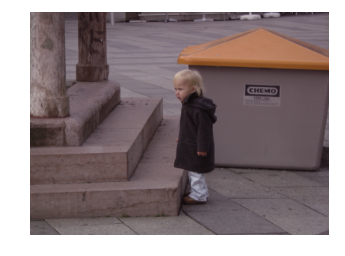
\includegraphics{https://raw.githubusercontent.com/cloudmesh/classes/master/docs/source/notebooks/files/image03.png}\strut
\end{minipage} & \begin{minipage}[t]{0.31\columnwidth}\raggedright\strut
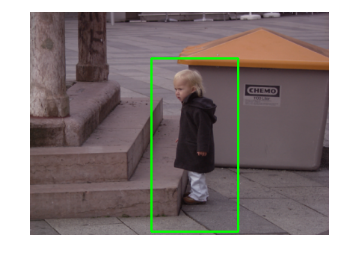
\includegraphics{https://raw.githubusercontent.com/cloudmesh/classes/master/docs/source/notebooks/files/image05.png}\strut
\end{minipage}\tabularnewline
\bottomrule
\end{longtable}

\begin{longtable}[]{@{}ll@{}}
\toprule
\begin{minipage}[b]{0.22\columnwidth}\raggedright\strut
Original\strut
\end{minipage} & \begin{minipage}[b]{0.50\columnwidth}\raggedright\strut
Pedestrian and Face/eyes Detected\strut
\end{minipage}\tabularnewline
\midrule
\endhead
\begin{minipage}[t]{0.22\columnwidth}\raggedright\strut
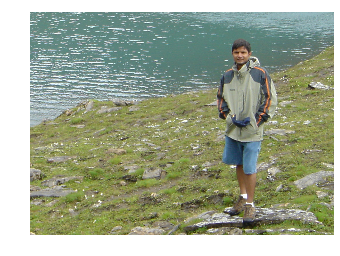
\includegraphics{https://raw.githubusercontent.com/cloudmesh/classes/master/docs/source/notebooks/files/image06.png}\strut
\end{minipage} & \begin{minipage}[t]{0.50\columnwidth}\raggedright\strut
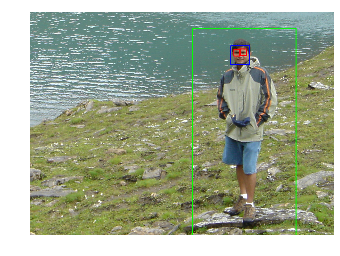
\includegraphics{https://raw.githubusercontent.com/cloudmesh/classes/master/docs/source/notebooks/files/image04.png}\strut
\end{minipage}\tabularnewline
\bottomrule
\end{longtable}

\subsection{Introduction}\label{introduction}

Human (pedestrian) detection and face detection have been studied during
the last several years and models for them have improved along with
Histograms of Oriented Gradients (HOG) for Human Detection {[}1{]}.
OpenCV is a Computer Vision library including the SVM classifier and the
HOG object detector for pedestrian detection and INRIA Person Dataset
{[}2{]} is one of popular samples for both training and testing
purposes. In this document, we deploy Apache Spark on Mesos clusters to
train and apply detection models from OpenCV using Python API.

\subsubsection{INRIA Person Dataset}\label{inria-person-dataset}

This dataset contains positive and negative images for training and test
purposes with annotation files for upright persons in each image. 288
positive test images, 453 negative test images, 614 positive training
images and 1218 negative training images are included along with
normalized 64x128 pixel formats. 970MB dataset is available to download
{[}3{]}.

\subsubsection{HOG with SVM model}\label{hog-with-svm-model}

Histogram of Oriented Gradient (HOG) and Support Vector Machine (SVM)
are used as object detectors and classifiers and built-in python
libraries from OpenCV provide these models for human detection.

\subsubsection{Ansible Automation Tool}\label{ansible-automation-tool}

Ansible is a python tool to install/configure/manage software on
multiple machines with JSON files where system descriptions are defined.
There are reasons why we use Ansible:

\begin{itemize}
\tightlist
\item
  Expandable: Leverages Python (default) but modules can be written in
  any language
\item
  Agentless: no setup required on managed node
\item
  Security: Allows deployment from user space; uses ssh for
  authentication
\item
  Flexibility: only requires ssh access to privileged user
\item
  Transparency: YAML Based script files express the steps of installing
  and configuring software
\item
  Modularity: Single Ansible Role (should) contain all required commands
  and variables to deploy software package independently
\item
  Sharing and portability: roles are available from source (github,
  bitbucket, gitlab, etc) or the Ansible Galaxy portal
\end{itemize}

We use Ansible roles to install software packages for Humand and Face
Detection which requires to run OpenCV Python libraries on Apache Mesos
with a cluster configuration. Dataset is also downloaded from the web
using an ansible role.

\subsection{Deployment by Ansible}\label{deployment-by-ansible}

Ansible is to deploy applications and build clusters for
batch-processing large datasets towards target machines e.g. VM
instances on OpenStack and we use ansible roles with \emph{include}
directive to organize layers of big data software stacks (BDSS). Ansible
provides abstractions by Playbook Roles and reusability by Include
statements. We define X application in X Ansible Role, for example, and
use include statements to combine with other applications e.g. Y or Z.
The layers exist in sub directories (see below) to add modularity to
your Ansible deployment. For example, there are five roles used in this
example that are Apache Mesos in a scheduler layer, Apache Spark in a
processing layer, a OpenCV library in an application layer, INRIA Person
Dataset in a dataset layer and a python script for human and face
detection in an analytics layer. If you have an additional software
package to add, you can simply add a new role in a main ansible playbook
with \emph{include} directive. With this, your Ansible playbook
maintains simple but flexible to add more roles without having a large
single file which is getting difficult to read when it deploys more
applications on multiple layers. The main Ansible playbook runs Ansible
roles in order which look like:

\begin{verbatim}
---
include: sched/00-mesos.yml
include: proc/01-spark.yml
include: apps/02-opencv.yml
include: data/03-inria-dataset.yml
Include: anlys/04-human-face-detection.yml
\end{verbatim}

Directory names e.g. sched, proc, data, or anlys indicate BDSS layers
like: - sched: scheduler layer - proc: data processing layer - apps:
application layer - data: dataset layer - anlys: analytics layer and two
digits in the filename indicate an order of roles to be run.

\subsection{Cloudmesh for
Provisioning}\label{cloudmesh-for-provisioning}

It is assumed that virtual machines are created by cloudmesh, the cloud
management software. For example on OpenStack,

\texttt{cm\ cluster\ create\ -N=6}

command starts a set of virtual machine instances. The number of
machines and groups for clusters e.g. namenodes and datanodes are
defined in the Ansible inventory file, a list of target machines with
groups, which will be generated once machines are ready to use by
cloudmesh. Ansible roles install software and dataset on virtual
clusters after that stage.

\subsection{Roles Explained for
Installation}\label{roles-explained-for-installation}

Mesos role is installed first as a scheduler layer for masters and
slaves where mesos-master runs on the masters group and mesos-slave runs
on the slaves group. Apache Zookeeper is included in the mesos role
therefore mesos slaves find an elected mesos leader for the
coordination. Spark, as a data processing layer, provides two options
for distributed job processing, batch job processing via a cluster mode
and real-time processing via a client mode. The Mesos dispatcher runs on
a masters group to accept a batch job submission and Spark interactive
shell, which is the client mode, provides real-time processing on any
node in the cluster. Either way, Spark is installed later to detect a
master (leader) host for a job submission. Other roles for OpenCV, INRIA
Person Dataset and Human and Face Detection Python applications are
followed by.

The following software are expected in the stacks according to the
\href{https://github.com/futuresystems/pedestrian-and-face-detection}{github}:

\begin{itemize}
\tightlist
\item
  mesos cluster (master, worker)
\item
  spark (with dispatcher for mesos cluster mode)
\item
  openCV
\item
  zookeeper
\item
  INRIA Person Dataset
\item
  Detection Analytics in Python
\item
  {[}1{]} Dalal, Navneet, and Bill Triggs. ``Histograms of oriented
  gradients for human detection.'' 2005 IEEE Computer Society Conference
  on Computer Vision and Pattern Recognition (CVPR'05). Vol. 1. IEEE,

  2005. {[}pdf{]}
\item
  {[}2{]} \url{http://pascal.inrialpes.fr/data/human/}
\item
  {[}3{]}
  \url{ftp://ftp.inrialpes.fr/pub/lear/douze/data/INRIAPerson.tar}
\item
  {[}4{]} \url{https://docs.python.org/2/library/configparser.html}
\end{itemize}

\subsubsection{Server groups for Masters/Slaves by Ansible
inventory}\label{server-groups-for-mastersslaves-by-ansible-inventory}

We may separate compute nodes in two groups: masters and workers
therefore Mesos masters and zookeeper quorums manage job requests and
leaders and workers run actual tasks. Ansible needs group definitions in
their inventory therefore software installation associated with a proper
part can be completed.

Example of Ansible Inventory file (inventory.txt)

\begin{verbatim}
[masters]
10.0.5.67
10.0.5.68
10.0.5.69
[slaves]
10.0.5.70
10.0.5.71
10.0.5.72
\end{verbatim}

\subsection{Instructions for
Deployment}\label{instructions-for-deployment}

The following commands complete NIST Pedestrian and Face Detection
deployment on OpenStack.

\subsubsection{Cloning Pedestrian Detection Repository from
Github}\label{cloning-pedestrian-detection-repository-from-github}

Roles are included as submodules which require \texttt{-\/-recursive}
option to checkout them all.

\begin{verbatim}
!git clone --recursive https://github.com/futuresystems/pedestrian-and-face-detection.git
\end{verbatim}

Change the following variable with actual ip addresses:

\begin{verbatim}
sample_inventory="""[masters]
10.0.5.67
10.0.5.68
10.0.5.69
[slaves]
10.0.5.70
10.0.5.71
10.0.5.72"""
\end{verbatim}

Create a \texttt{inventory.txt} file with the variable in your local
directory.

\begin{verbatim}
!printf "$sample_inventory" > inventory.txt
!cat inventory.txt
\end{verbatim}

Add \texttt{ansible.cfg} file with options for ssh host key checking and
login name.

\begin{verbatim}
ansible_config="""[defaults]
host_key_checking=false
remote_user=ubuntu"""
!printf "$ansible_config" > ansible.cfg
!cat ansible.cfg
\end{verbatim}

Check accessibility by ansible ping like:

\begin{verbatim}
!ansible -m ping -i inventory.txt all
\end{verbatim}

Make sure that you have a correct ssh key in your account otherwise you
may encounter `FAILURE' in the ping test above.

\subsubsection{Ansible Playbook}\label{ansible-playbook}

We use a main ansible playbook to deploy software packages for NIST
Pedestrian and Face detection which includes: - mesos - spark -zookeeper
- opencv - INRIA Person dataset - Python script for the detection

\begin{verbatim}
!cd pedestrian-and-face-detection/ && ansible-playbook -i ../inventory.txt site.yml
\end{verbatim}

The installation may take 30 minutes or an hour to complete.

\subsection{OpenCV in Python}\label{opencv-in-python}

Before we run our code for this project, let's try OpenCV first to see
how it works.

\subsubsection{Import cv2}\label{import-cv2}

Let's import opencv python module and we will use images from the online
database image-net.org to test OpenCV image recognition.

\begin{verbatim}
import cv2
\end{verbatim}

Let's download a mailbox image with a red color to see if opencv
identifies the shape with a color. The example file in this tutorial is:

\begin{verbatim}
!curl http://farm4.static.flickr.com/3061/2739199963_ee78af76ef.jpg > mailbox.jpg
\end{verbatim}

\begin{quote}
100 167k 100 167k 0 0 686k 0 --:--:-- --:--:-- --:--:-- 684k
\end{quote}

\begin{verbatim}
%matplotlib inline
\end{verbatim}

\begin{verbatim}
from IPython.display import Image
mailbox_image = "mailbox.jpg"
Image(filename=mailbox_image)
\end{verbatim}

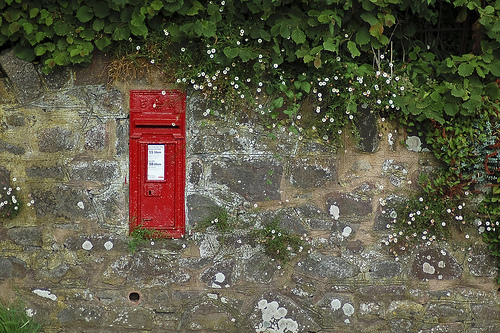
\includegraphics{facedetection_files/facedetection_46_0.jpeg}

You can try other images. Check out the image-net.org for mailbox
images: \url{http://image-net.org/synset?wnid=n03710193}

\subsubsection{Image Detection}\label{image-detection}

Just for a test, let's try to detect a red color shaped mailbox using
opencv python functions.

There are key functions that we use: * cvtColor: to convert a color
space of an image * inRange: to detect a mailbox based on the range of
red color pixel values * np.array: to define the range of red color
using a Numpy library for better calculation * findContours: to find a
outline of the object * bitwise\_and: to black-out the area of contours
found

\begin{verbatim}
import numpy as np
import matplotlib.pyplot as plt

# imread for loading an image
img = cv2.imread(mailbox_image)
# cvtColor for color conversion
hsv = cv2.cvtColor(img,cv2.COLOR_BGR2HSV)

# define range of red color in hsv
lower_red1 = np.array([0, 50, 50])
upper_red1 = np.array([10, 255, 255])
lower_red2 = np.array([170, 50, 50])
upper_red2 = np.array([180, 255, 255])

# threshold the hsv image to get only red colors
mask1 = cv2.inRange(hsv, lower_red1, upper_red1)
mask2 = cv2.inRange(hsv, lower_red2, upper_red2)
mask = mask1 + mask2

# find a red color mailbox from the image
im2, contours,hierarchy = cv2.findContours(mask, cv2.RETR_TREE, cv2.CHAIN_APPROX_SIMPLE)

# bitwise_and to remove other areas in the image except the detected object
res = cv2.bitwise_and(img, img, mask = mask)

# turn off - x, y axis bar
plt.axis("off")
# text for the masked image
cv2.putText(res, "masked image", (20,300), cv2.FONT_HERSHEY_SIMPLEX, 2, (255,255,255))
# display
plt.imshow(cv2.cvtColor(res, cv2.COLOR_BGR2RGB))
plt.show()
\end{verbatim}


\includegraphics{facedetection_files/facedetection_49_0.png}

The red color mailbox is left alone in the image which we wanted to find
in this example by opencv functions. You can try other images with
different colors to detect the different shape of objects using
findContours and inRange from opencv.

For more information, see the useful links below.

\begin{itemize}
\tightlist
\item
  contours features:
  \url{http://docs.opencv.org/3.1.0/dd/d49/tutorial/_py/_contour/_features.html}
\item
  contours:
  \url{http://docs.opencv.org/3.1.0/d4/d73/tutorial/_py/_contours/_begin.html}
\item
  red color in hsv:
  \url{http://stackoverflow.com/questions/30331944/finding-red-color-using-python-opencv}
\item
  inrange:
  \url{http://docs.opencv.org/master/da/d97/tutorial/_threshold/_inRange.html}
\item
  inrange:
  \url{http://docs.opencv.org/3.0-beta/doc/py/_tutorials/py/_imgproc/py/_colorspaces/py/_colorspaces.html}
\item
  numpy:
  \url{http://docs.opencv.org/3.0-beta/doc/py/_tutorials/py/_core/py/_basic/_ops/py/_basic/_ops.html}
\end{itemize}

\subsection{Human and Face Detection in
OpenCV}\label{human-and-face-detection-in-opencv}

\subsubsection{INRIA Person Dataset}\label{inria-person-dataset-1}

We use INRIA Person dataset to detect upright people and faces in images
in this example. Let's download it first.

\begin{verbatim}
!curl ftp://ftp.inrialpes.fr/pub/lear/douze/data/INRIAPerson.tar > INRIAPerson.tar
\end{verbatim}

\begin{quote}
100 969M 100 969M 0 0 8480k 0 0:01:57 0:01:57 --:--:-- 12.4M
\end{quote}

\begin{verbatim}
!tar xvf INRIAPerson.tar > logfile && tail logfile
\end{verbatim}

\subsubsection{Face Detection using Haar
Cascades}\label{face-detection-using-haar-cascades}

This section is prepared based on the opencv-python tutorial:
\url{http://docs.opencv.org/3.1.0/d7/d8b/tutorial/_py/_face/_detection.html\#gsc.tab=0}

There is a pre-trained classifier for face detection, download it from
here:

\begin{verbatim}
!curl https://raw.githubusercontent.com/opencv/opencv/master/data/haarcascades/haarcascade_frontalface_default.xml > haarcascade_frontalface_default.xml
\end{verbatim}

\begin{quote}
100 908k 100 908k 0 0 2225k 0 --:--:-- --:--:-- --:--:-- 2259k
\end{quote}

This classifier XML file will be used to detect faces in images. If you
like to create a new classifier, find out more information about
training from here:
\url{http://docs.opencv.org/3.1.0/dc/d88/tutorial/_traincascade.html}

\subsubsection{Face Detection Python Code
Snippet}\label{face-detection-python-code-snippet}

Now, we detect faces from the first five images using the classifier.

\begin{verbatim}
# import the necessary packages
from __future__ import print_function
import numpy as np
import cv2
from os import listdir
from os.path import isfile, join
import matplotlib.pyplot as plt

mypath = "INRIAPerson/Test/pos/"
face_cascade = cv2.CascadeClassifier('haarcascade_frontalface_default.xml')

onlyfiles = [join(mypath, f) for f in listdir(mypath) if isfile(join(mypath, f))]

cnt = 0
for filename in onlyfiles:
    image = cv2.imread(filename)
    image_grayscale = cv2.cvtColor(image, cv2.COLOR_BGR2GRAY)
    faces = face_cascade.detectMultiScale(image_grayscale, 1.3, 5)
    if len(faces) == 0:
        continue

    cnt_faces = 1
    for (x,y,w,h) in faces:
        cv2.rectangle(image,(x,y),(x+w,y+h),(255,0,0),2)
        cv2.putText(image, "face" + str(cnt_faces), (x,y-10), cv2.FONT_HERSHEY_SIMPLEX, 1, (0,0,0), 2)
        plt.figure()
        plt.axis("off")
        plt.imshow(cv2.cvtColor(image[y:y+h, x:x+w], cv2.COLOR_BGR2RGB))
        cnt_faces += 1
    plt.figure()
    plt.axis("off")
    plt.imshow(cv2.cvtColor(image, cv2.COLOR_BGR2RGB))        
    cnt = cnt + 1
    if cnt == 5:
        break
\end{verbatim}

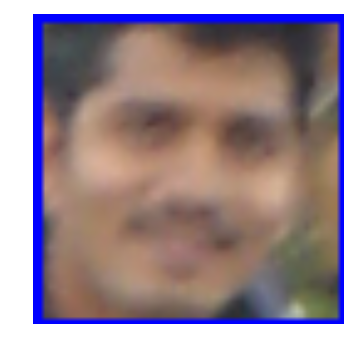
\includegraphics{facedetection_files/facedetection_59_0.png}

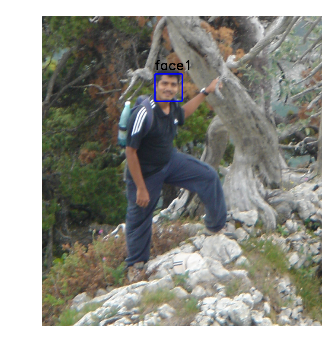
\includegraphics{facedetection_files/facedetection_59_1.png}

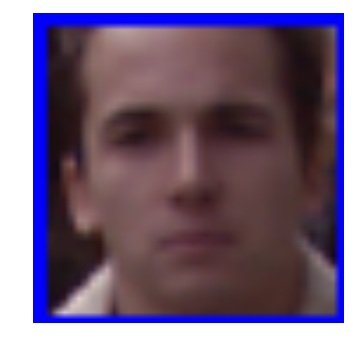
\includegraphics{facedetection_files/facedetection_59_2.png}

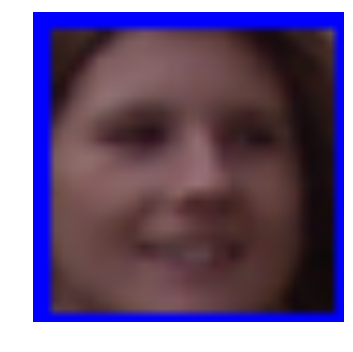
\includegraphics{facedetection_files/facedetection_59_3.png}

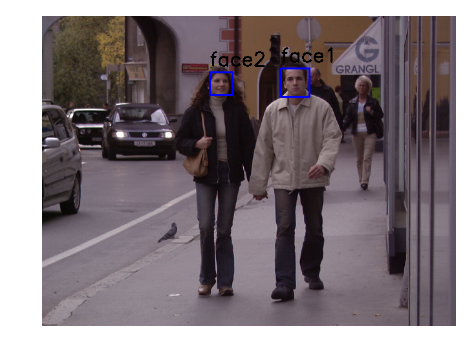
\includegraphics{facedetection_files/facedetection_59_4.png}

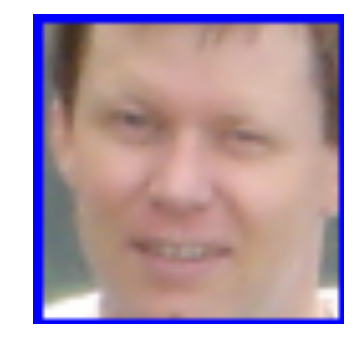
\includegraphics{facedetection_files/facedetection_59_5.png}

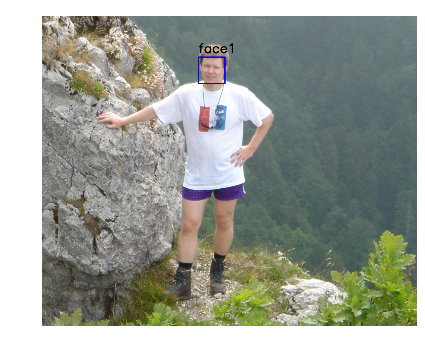
\includegraphics{facedetection_files/facedetection_59_6.png}

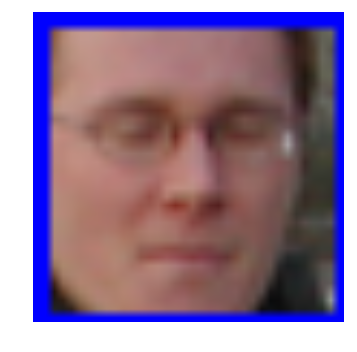
\includegraphics{facedetection_files/facedetection_59_7.png}

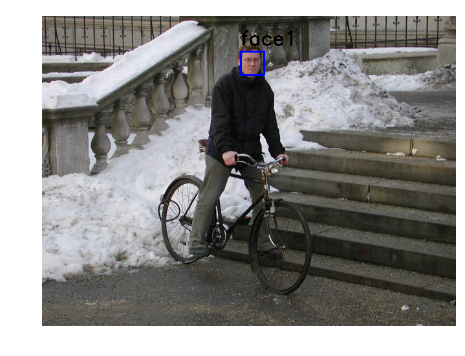
\includegraphics{facedetection_files/facedetection_59_8.png}

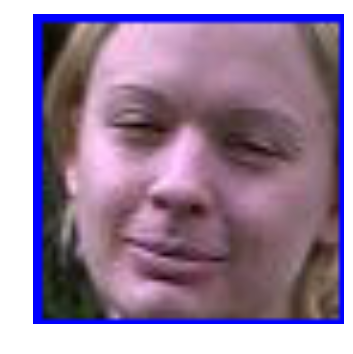
\includegraphics{facedetection_files/facedetection_59_9.png}

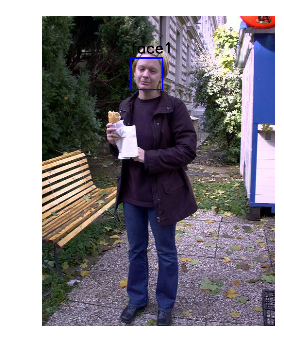
\includegraphics{facedetection_files/facedetection_59_10.png}

\subsection{Pedestrian Detection using HOG
Descriptor}\label{pedestrian-detection-using-hog-descriptor}

We will use Histogram of Oriented Gradients (HOG) to detect a upright
person from images.

\subsubsection{Python Code Snippet}\label{python-code-snippet}

\begin{verbatim}
# initialize the HOG descriptor/person detector
hog = cv2.HOGDescriptor()
hog.setSVMDetector(cv2.HOGDescriptor_getDefaultPeopleDetector())

cnt = 0
for filename in onlyfiles:
    img = cv2.imread(filename)
    orig = img.copy()
    gray = cv2.cvtColor(img, cv2.COLOR_BGR2GRAY)

    # detect people in the image
    (rects, weights) = hog.detectMultiScale(img, winStride=(8, 8),
    padding=(16, 16), scale=1.05)

    # draw the final bounding boxes
    for (x, y, w, h) in rects:
        cv2.rectangle(img, (x, y), (x + w, y + h), (0, 255, 0), 2)

    plt.figure()
    plt.axis("off")
    plt.imshow(cv2.cvtColor(orig, cv2.COLOR_BGR2RGB))
    plt.figure()
    plt.axis("off")
    plt.imshow(cv2.cvtColor(img, cv2.COLOR_BGR2RGB))
    cnt = cnt + 1
    if cnt == 5:
        break
\end{verbatim}

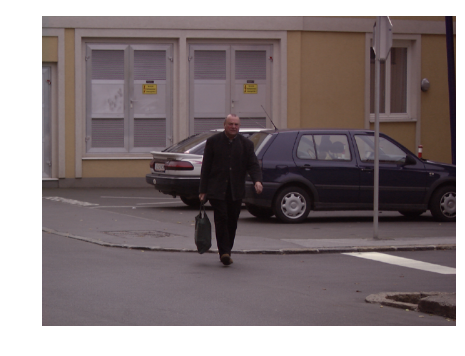
\includegraphics{facedetection_files/facedetection_62_0.png}

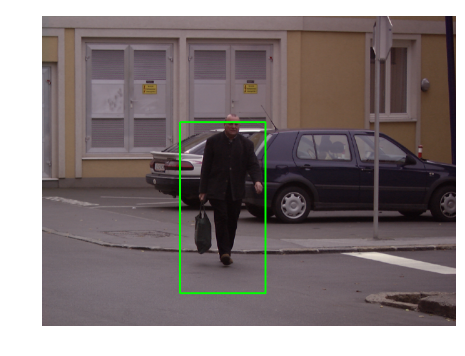
\includegraphics{facedetection_files/facedetection_62_1.png}

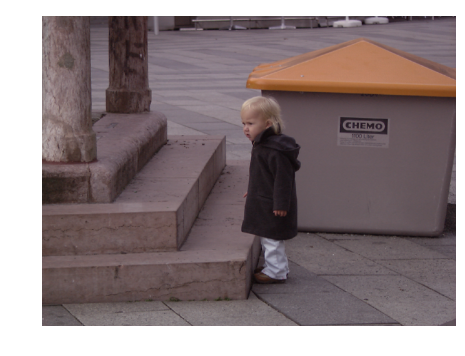
\includegraphics{facedetection_files/facedetection_62_2.png}

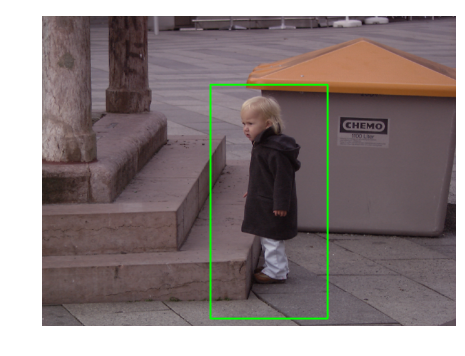
\includegraphics{facedetection_files/facedetection_62_3.png}

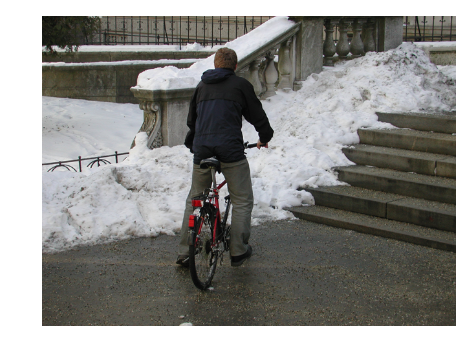
\includegraphics{facedetection_files/facedetection_62_4.png}

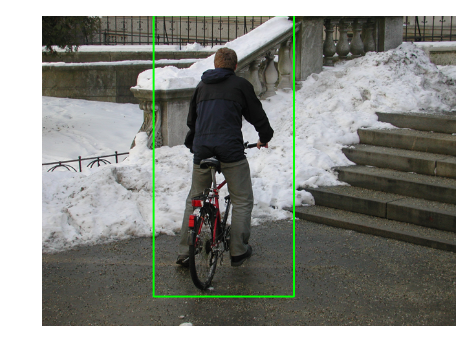
\includegraphics{facedetection_files/facedetection_62_5.png}

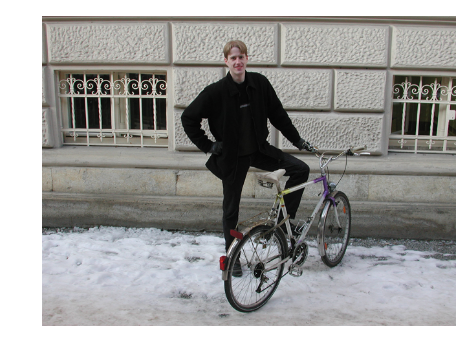
\includegraphics{facedetection_files/facedetection_62_6.png}

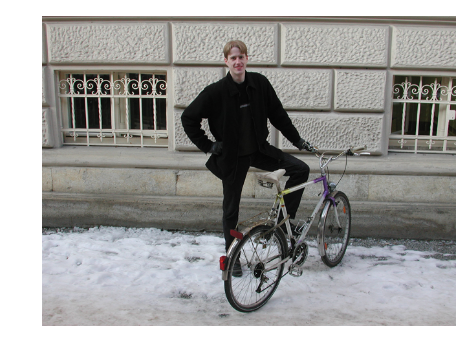
\includegraphics{facedetection_files/facedetection_62_7.png}

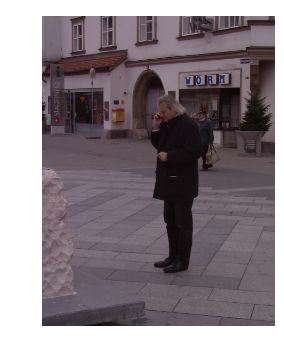
\includegraphics{facedetection_files/facedetection_62_8.png}

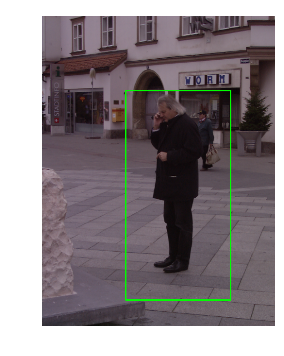
\includegraphics{facedetection_files/facedetection_62_9.png}

\subsection{Processing by Apache
Spark}\label{processing-by-apache-spark}

INRIA Person dataset provides 100+ images and Spark can be used for
image processing in parallel. We load 288 images from ``Test/pos''
directory.

Spark provides a special object `sc' to connect between a spark cluster
and functions in python code. Therefore, we can run python functions in
parallel to detet objects in this example.

\begin{itemize}
\tightlist
\item
  \emph{map} function is used to process pedestrian and face detection
  per image from the parallelize() function of `sc' spark context.
\item
  \emph{collect} fonction merges results in an array.
\end{itemize}

\begin{verbatim}
def apply_batch(imagePath):
        import cv2
        import numpy as np
        # initialize the HOG descriptor/person detector
        hog = cv2.HOGDescriptor()
        hog.setSVMDetector(cv2.HOGDescriptor_getDefaultPeopleDetector())
        image = cv2.imread(imagePath)
        # detect people in the image
        (rects, weights) = hog.detectMultiScale(image, winStride=(8, 8),
            padding=(16, 16), scale=1.05)
        # draw the final bounding boxes
        for (x, y, w, h) in rects:
            cv2.rectangle(image, (x, y), (x + w, y + h), (0, 255, 0), 2)
        return image
\end{verbatim}

\subsubsection{Parallelize in Spark
Context}\label{parallelize-in-spark-context}

The list of image files is given to parallelize.

\begin{verbatim}
pd = sc.parallelize(onlyfiles)
\end{verbatim}

\subsubsection{Map Function
(apply\_batch)}\label{map-function-apply_batch}

The `apply\_batch' function that we created above is given to map
function to process in a spark cluster.

\begin{verbatim}
pdc = pd.map(apply_batch)
\end{verbatim}

\subsubsection{Collect Function}\label{collect-function}

The result of each map process is merged to an array.

\begin{verbatim}
result = pdc.collect()
\end{verbatim}

\subsection{Results for 100+ images by Spark
Cluster}\label{results-for-100-images-by-spark-cluster}

\begin{verbatim}
for image in result:
    plt.figure()
    plt.axis("off")
    plt.imshow(cv2.cvtColor(image, cv2.COLOR_BGR2RGB))
\end{verbatim}

\section{Instalation}\label{instalation}

Scikit-learn requires:

\begin{verbatim}
Python (>= 2.6 or >= 3.3),
NumPy (>= 1.6.1),
SciPy (>= 0.9).
\end{verbatim}

If you already have a working installation of numpy and scipy, the
easiest way to install scikit-learn is using pip

\begin{verbatim}
! pip install numpy
\end{verbatim}

\begin{verbatim}
! pip install scipy -U
\end{verbatim}

\begin{verbatim}
! pip install -U scikit-learn
\end{verbatim}

\subsection{Import}\label{import}

\begin{verbatim}
from time import time
import numpy as np
import matplotlib.pyplot as plt

from sklearn import metrics
from sklearn.cluster import KMeans
from sklearn.datasets import load_digits
from sklearn.decomposition import PCA
from sklearn.preprocessing import scale
\end{verbatim}

\subsection{Create samples}\label{create-samples}

\begin{verbatim}
np.random.seed(42)

digits = load_digits()
data = scale(digits.data)

n_samples, n_features = data.shape
n_digits = len(np.unique(digits.target))
labels = digits.target

sample_size = 300

print("n_digits: %d, \t n_samples %d, \t n_features %d"
      % (n_digits, n_samples, n_features))


print(79 * '_')
print('% 9s' % 'init'
      '    time  inertia    homo   compl  v-meas     ARI AMI  silhouette')


def bench_k_means(estimator, name, data):
    t0 = time()
    estimator.fit(data)
    print('% 9s   %.2fs    %i   %.3f   %.3f   %.3f   %.3f   %.3f    %.3f'
          % (name, (time() - t0), estimator.inertia_,
             metrics.homogeneity_score(labels, estimator.labels_),
             metrics.completeness_score(labels, estimator.labels_),
             metrics.v_measure_score(labels, estimator.labels_),
             metrics.adjusted_rand_score(labels, estimator.labels_),
             metrics.adjusted_mutual_info_score(labels,  estimator.labels_),
             metrics.silhouette_score(data, estimator.labels_,
                                      metric='euclidean',
                                      sample_size=sample_size)))

bench_k_means(KMeans(init='k-means++', n_clusters=n_digits, n_init=10),
              name="k-means++", data=data)

bench_k_means(KMeans(init='random', n_clusters=n_digits, n_init=10),
              name="random", data=data)

# in this case the seeding of the centers is deterministic, hence we run the
# kmeans algorithm only once with n_init=1
pca = PCA(n_components=n_digits).fit(data)
bench_k_means(KMeans(init=pca.components_, 
                     n_clusters=n_digits, n_init=1),
              name="PCA-based",
              data=data)
print(79 * '_')
\end{verbatim}

\section{Visualize}\label{visualize}

\begin{verbatim}
reduced_data = PCA(n_components=2).fit_transform(data)
kmeans = KMeans(init='k-means++', n_clusters=n_digits, n_init=10)
kmeans.fit(reduced_data)

# Step size of the mesh. Decrease to increase the quality of the VQ.
h = .02     # point in the mesh [x_min, x_max]x[y_min, y_max].

# Plot the decision boundary. For that, we will assign a color to each
x_min, x_max = reduced_data[:, 0].min() - 1, reduced_data[:, 0].max() + 1
y_min, y_max = reduced_data[:, 1].min() - 1, reduced_data[:, 1].max() + 1
xx, yy = np.meshgrid(np.arange(x_min, x_max, h), np.arange(y_min, y_max, h))

# Obtain labels for each point in mesh. Use last trained model.
Z = kmeans.predict(np.c_[xx.ravel(), yy.ravel()])

# Put the result into a color plot
Z = Z.reshape(xx.shape)
plt.figure(1)
plt.clf()
plt.imshow(Z, interpolation='nearest',
           extent=(xx.min(), xx.max(), yy.min(), yy.max()),
           cmap=plt.cm.Paired,
           aspect='auto', origin='lower')

plt.plot(reduced_data[:, 0], reduced_data[:, 1], 'k.', markersize=2)
# Plot the centroids as a white X
centroids = kmeans.cluster_centers_
plt.scatter(centroids[:, 0], centroids[:, 1],
            marker='x', s=169, linewidths=3,
            color='w', zorder=10)
plt.title('K-means clustering on the digits dataset (PCA-reduced data)\n'
          'Centroids are marked with white cross')
plt.xlim(x_min, x_max)
plt.ylim(y_min, y_max)
plt.xticks(())
plt.yticks(())
plt.show()
\end{verbatim}

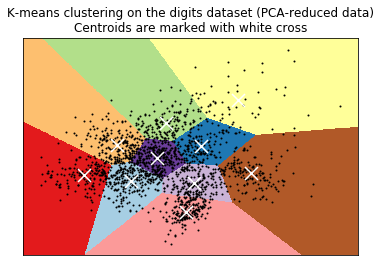
\includegraphics{scikit-learn-k-means_files/scikit-learn-k-means_10_0.png}

\section{Python Fingerprint Example}\label{python-fingerprint-example}

Python is a flexible and popular language for running data analysis
pipelines. In this tutorial we will implement a solution for a
fingerprint matching.

\subsection{Overview}\label{overview}

Fingerprint recognition refers to the automated method for verifying a
match between two fingerprints and that is used to identify individuals
and verify their identity. Fingerprints (Figure 1) are the most widely
used form of biometric used to identify individuals.

\begin{figure}
\centering
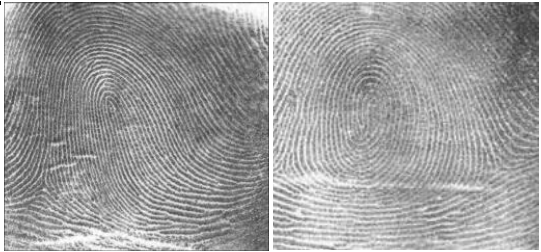
\includegraphics{./fingerprints.png}
\caption{Fingerprints}
\end{figure}

The automated fingerprint matching generally required the detection of
different fingerprint features (aggregate characteristics of ridges, and
minutia points) and then the use of fingerprint matching algorithm,
which can do both one-to- one and one-to- many matching operations.
Based on the number of matches a proximity score (distance or
similarity) can be calculated.

We use the following NIST dataset for the study:

Special Database 14 - NIST Mated Fingerprint Card Pairs 2.
(\url{http://www.nist.gov/itl/iad/ig/special/_dbases.cfm})

\subsection{Objectives}\label{objectives}

Match the fingerprint images from a probe set to a gallery set and
report the match scores.

\subsection{Prerequisites}\label{prerequisites}

For this work we will use the following algorithms:

\begin{itemize}
\tightlist
\item
  MINDTCT: The NIST minutiae detector, which automatically locates and
  records ridge ending and bifurcations in a fingerprint image.
  (\url{http://www.nist.gov/itl/iad/ig/nbis.cfm})
\item
  BOZORTH3: A NIST fingerprint matching algorithm, which is a minutiae
  based fingerprint-matching algorithm. It can do both one-to- one and
  one-to- many matching operations.
  (\url{http://www.nist.gov/itl/iad/ig/nbis.cfm})
\end{itemize}

In order to follow along, you must have the NBIS tools which provide
\texttt{mindtct} and \texttt{bozorth3} installed. If you are on Ubuntu
16.04 Xenial, the following steps will accomplish this:

\begin{verbatim}
$ sudo apt-get update -qq
$ sudo apt-get install -y build-essential cmake unzip
$ wget "http://nigos.nist.gov:8080/nist/nbis/nbis_v5_0_0.zip"
$ unzip -d nbis nbis_v5_0_0.zip
$ cd nbis/Rel_5.0.0
$ ./setup.sh /usr/local --without-X11
$ sudo make
\end{verbatim}

\subsection{Implementation}\label{implementation}

\begin{enumerate}
\def\labelenumi{\arabic{enumi}.}
\tightlist
\item
  Fetch the fingerprint images from the web
\item
  Call out to external programs to prepare and compute the match scoreds
\item
  Store the results in a database
\item
  Generate a plot to identify likely matches.
\end{enumerate}

\begin{verbatim}
from __future__ import print_function
\end{verbatim}

\begin{verbatim}
import urllib
import zipfile
import hashlib
\end{verbatim}

We'll be interacting with the operating system and manipulating files
and their pathnames.

\begin{verbatim}
import os.path
import os
import sys
import shutil
import tempfile
\end{verbatim}

Some general usefull utilities

\begin{verbatim}
import itertools
import functools
import types
from pprint import pprint
\end{verbatim}

Using the \texttt{attrs} library provides some nice shortcuts to
defining objects

\begin{verbatim}
import attr
\end{verbatim}

\begin{verbatim}
import sys
\end{verbatim}

We'll be randomly dividing the entire dataset, based on user input, into
the probe and gallery stets

\begin{verbatim}
import random
\end{verbatim}

We'll need to call out to the NBIS software. We'll also be using
multiple processes to take advantage of all the cores on our machine

\begin{verbatim}
import subprocess
import multiprocessing
\end{verbatim}

As for plotting, we'll use \texttt{matplotlib}, though there are many
alternatives.

\begin{verbatim}
import matplotlib.pyplot as plt
import pandas as pd
import numpy as np
\end{verbatim}

Finally, we'll write the results to a database.

\begin{verbatim}
import sqlite3
\end{verbatim}

\subsection{Utility functions}\label{utility-functions}

Next, we'll define some utility functions:

\begin{verbatim}
def take(n, iterable):
    "Returns a generator of the first **n** elements of an iterable"
    return itertools.islice(iterable, n )


def zipWith(function, *iterables):
    "Zip a set of **iterables** together and apply **function** to each tuple"
    for group in itertools.izip(*iterables):
        yield function(*group)


def uncurry(function):
    "Transforms an N-arry **function** so that it accepts a single parameter of an N-tuple"
    @functools.wraps(function)
    def wrapper(args):
        return function(*args)
    return wrapper


def fetch_url(url, sha256, prefix='.', checksum_blocksize=2**20, dryRun=False):
    """Download a url.

    :param url: the url to the file on the web
    :param sha256: the SHA-256 checksum. Used to determine if the file was previously downloaded.
    :param prefix: directory to save the file
    :param checksum_blocksize: blocksize to used when computing the checksum
    :param dryRun: boolean indicating that calling this function should do nothing
    :returns: the local path to the downloaded file
    :rtype:

    """

    if not os.path.exists(prefix):
        os.makedirs(prefix)

    local = os.path.join(prefix, os.path.basename(url))

    if dryRun: return local

    if os.path.exists(local):
        print ('Verifying checksum')
        chk = hashlib.sha256()
        with open(local, 'rb') as fd:
            while True:
                bits = fd.read(checksum_blocksize)
                if not bits: break
                chk.update(bits)
        if sha256 == chk.hexdigest():
            return local

    print ('Downloading', url)

    def report(sofar, blocksize, totalsize):
        msg = '{}%\r'.format(100 * sofar * blocksize / totalsize, 100)
        sys.stderr.write(msg)

    urllib.urlretrieve(url, local, report)

    return local
\end{verbatim}

\subsection{Dataset}\label{dataset}

We'll now define some global parameters

First, the fingerprint dataset

\begin{verbatim}
DATASET_URL = 'https://s3.amazonaws.com/nist-srd/SD4/NISTSpecialDatabase4GrayScaleImagesofFIGS.zip'
DATASET_SHA256 = '4db6a8f3f9dc14c504180cbf67cdf35167a109280f121c901be37a80ac13c449'
\end{verbatim}

We'll define how to download the dataset. This function is general
enough that it could be used to retrieve most files, but we'll default
it to use the values from above.

\begin{verbatim}
def prepare_dataset(url=None, sha256=None, prefix='.', skip=False):
    url = url or DATASET_URL
    sha256 = sha256 or DATASET_SHA256
    local = fetch_url(url, sha256=sha256, prefix=prefix, dryRun=skip)

    if not skip:
        print ('Extracting', local, 'to', prefix)
        with zipfile.ZipFile(local, 'r') as zip:
            zip.extractall(prefix)

    name, _ = os.path.splitext(local)
    return name


def locate_paths(path_md5list, prefix):
    with open(path_md5list) as fd:
        for line in itertools.imap(str.strip, fd):
            parts = line.split()
            if not len(parts) == 2: continue
            md5sum, path = parts
            chksum = Checksum(value=md5sum, kind='md5')
            filepath = os.path.join(prefix, path)
            yield Path(checksum=chksum, filepath=filepath)


def locate_images(paths):

    def predicate(path):
        _, ext = os.path.splitext(path.filepath)
        return ext in ['.png']

    for path in itertools.ifilter(predicate, paths):
        yield image(id=path.checksum.value, path=path)
\end{verbatim}

\subsection{Data Model}\label{data-model}

We'll define some classes so we have a nice API for working with the
dataflow. We set \texttt{slots=True} so that the resulting objects will
be more space-efficient.

\subsubsection{Utilities}\label{utilities}

\paragraph{Checksum}\label{checksum}

The checksum consists of the actual hash value (\texttt{value}) as well
as a string representing the hashing algorithm. The validator enforces
that the algorith can only be one of the listed acceptable methods

\begin{verbatim}
@attr.s(slots=True)
class Checksum(object):
  value = attr.ib()
  kind = attr.ib(validator=lambda o, a, v: v in 'md5 sha1 sha224 sha256 sha384 sha512'.split())
\end{verbatim}

\paragraph{Path}\label{path}

\texttt{Path}s refer to an image's filepath and associated
\texttt{Checksum}. We get the checksum ``for''free" since the MD5 hash
is provided for each image in the dataset.

\begin{verbatim}
@attr.s(slots=True)
class Path(object):
    checksum = attr.ib()
    filepath = attr.ib()
\end{verbatim}

\paragraph{Image}\label{image}

The start of the data pipeline is the image. An \texttt{image} has an
\texttt{id} (the md5 hash) and the path to the image.

\begin{verbatim}
@attr.s(slots=True)
class image(object):
    id = attr.ib()
    path = attr.ib()
\end{verbatim}

\subsubsection{Mindtct}\label{mindtct}

The next step in the pipeline is to apply the \texttt{mindtct} program
from NBIS. A \texttt{mindtct} object therefore represents the results of
applying \texttt{mindtct} on an \texttt{image}. The \texttt{xyt} output
is needed fo r the next step, and the \texttt{image} attribute
represents the image id.

\begin{verbatim}
@attr.s(slots=True)
class mindtct(object):
    image = attr.ib()
    xyt = attr.ib()

    def pretty(self):
        d = dict(id=self.image.id, path=self.image.path)
        return pprint(d)
\end{verbatim}

We need a way to construct a \texttt{mindtct} object from an
\texttt{image} object. A straightforward way of doing this would be to
have a \texttt{from\_image} \texttt{@staticmethod} or
\texttt{@classmethod}, but that doesn't work well with
\texttt{multiprocessing} as top-level functions work best as they need
to be serialized.

\begin{verbatim}
def mindtct_from_image(image):
    imgpath = os.path.abspath(image.path.filepath)
    tempdir = tempfile.mkdtemp()
    oroot = os.path.join(tempdir, 'result')

    cmd = ['mindtct', imgpath, oroot]

    try:
        subprocess.check_call(cmd)

        with open(oroot + '.xyt') as fd:
            xyt = fd.read()

        result = mindtct(image=image.id, xyt=xyt)
        return result

    finally:
        shutil.rmtree(tempdir)
\end{verbatim}

\subsubsection{Bozorth3}\label{bozorth3}

The final step in the pipeline is running the \texttt{bozorth3} from
NBIS. The \texttt{bozorth3} class represents the match being done:
tracking the ids of the probe and gallery images as well as the match
score.

Since we'll be writing these instance out to a database, we provide some
static methods for SQL statements. While there are many
Object-Relational-Model (ORM) libraries available for Python, this
approach keeps the current implementation simple.

\begin{verbatim}
@attr.s(slots=True)
class bozorth3(object):
    probe = attr.ib()
    gallery = attr.ib()
    score = attr.ib()

    @staticmethod
    def sql_stmt_create_table():
        return 'CREATE TABLE IF NOT EXISTS bozorth3' \
             + '(probe TEXT, gallery TEXT, score NUMERIC)'

    @staticmethod
    def sql_prepared_stmt_insert():
        return 'INSERT INTO bozorth3 VALUES (?, ?, ?)'

    def sql_prepared_stmt_insert_values(self):
        return self.probe, self.gallery, self.score
\end{verbatim}

In order to work well with \texttt{multiprocessing}, we define a class
representuing the input paramaters to \texttt{bozorth3} and a helper
function to run \texttt{bozorth3}. This way the pipeline definition can
be kept simple to a \texttt{map} to create the input and then a
\texttt{map} to run the program.

As NBIS \texttt{bozorth3} can be called to compare one-to-one or
one-to-many, we'll also dynamically choose between these approaches
depending on if the gallery attribute is a list or a single object.

\begin{verbatim}
@attr.s(slots=True)
class bozorth3_input(object):
    probe = attr.ib()
    gallery = attr.ib()

    def run(self):
        if isinstance(self.gallery, mindtct):
            return bozorth3_from_one_to_one(self.probe, self.gallery)
        elif isinstance(self.gallery, types.ListType):
            return bozorth3_from_one_to_many(self.probe, self.gallery)
        else:
            raise ValueError('Unhandled type for gallery: {}'.format(type(gallery)))
\end{verbatim}

The next is the top-level function to running \texttt{bozorth3}. It
accepts an instance of \texttt{bozorth3\_input}. The is implemented as a
simple top-level wrapper so that it can be easily passed to the
\texttt{multiprocessing} library.

\begin{verbatim}
def run_bozorth3(input):
    return input.run()
\end{verbatim}

\paragraph{Running Bozorth3}\label{running-bozorth3}

There are two cases to handle: 1. One-to-one probe to gallery sets 1.
One-to-many probe to gallery sets

Both approaches are implemented below. The implementations follow the
same pattern: 1. Create a temporary directory within with to work 1.
Write the probe and gallery images to files in the temporary directory
1. Call the \texttt{bozorth3} executable 1. The match score is written
to \texttt{stdout} which is captured and then parsed. 1. Return a
\texttt{bozorth3} instance for each match 1. Make sure to clean up the
temporary directory

\subparagraph{One-to-one}\label{one-to-one}

\begin{verbatim}
def bozorth3_from_one_to_one(probe, gallery):
    tempdir = tempfile.mkdtemp()
    probeFile = os.path.join(tempdir, 'probe.xyt')
    galleryFile = os.path.join(tempdir, 'gallery.xyt')

    with open(probeFile,   'wb') as fd: fd.write(probe.xyt)
    with open(galleryFile, 'wb') as fd: fd.write(gallery.xyt)

    cmd = ['bozorth3', probeFile, galleryFile]

    try:
        result = subprocess.check_output(cmd)
        score = int(result.strip())
        return bozorth3(probe=probe.image, gallery=gallery.image, score=score)
    finally:
        shutil.rmtree(tempdir)
\end{verbatim}

\subparagraph{One-to-many}\label{one-to-many}

\begin{verbatim}
def bozorth3_from_one_to_many(probe, galleryset):
    tempdir = tempfile.mkdtemp()
    probeFile = os.path.join(tempdir, 'probe.xyt')
    galleryFiles = [os.path.join(tempdir, 'gallery%d.xyt' % i)
                    for i,_ in enumerate(galleryset)]

    with open(probeFile, 'wb') as fd: fd.write(probe.xyt)
    for galleryFile, gallery in itertools.izip(galleryFiles, galleryset):
        with open(galleryFile, 'wb') as fd: fd.write(gallery.xyt)

    cmd = ['bozorth3', '-p', probeFile] + galleryFiles

    try:
        result = subprocess.check_output(cmd).strip()
        scores = map(int, result.split('\n'))
        return [bozorth3(probe=probe.image, gallery=gallery.image, score=score)
               for score, gallery in zip(scores, galleryset)]
    finally:
        shutil.rmtree(tempdir)
\end{verbatim}

\section{Plotting}\label{plotting}

For plotting we'll operate only on the database. We'll select a small
number of probe images and plot the score between them and the rest of
the gallery images.

The \texttt{mk\_short\_labels} helper function will be defined below.

\begin{verbatim}
def plot(dbfile, nprobes=10):
    conn = sqlite3.connect(dbfile)
    results = pd.read_sql(
        "SELECT DISTINCT probe FROM bozorth3 ORDER BY score LIMIT '%s'" % nprobes,
        con=conn
    )
    shortlabels = mk_short_labels(results.probe)
    plt.figure()

    for i, probe in results.probe.iteritems():
        stmt = 'SELECT gallery, score FROM bozorth3 WHERE probe = ? ORDER BY gallery DESC'
        matches = pd.read_sql(stmt, params=(probe,), con=conn)
        xs = np.arange(len(matches), dtype=np.int)
        plt.plot(xs, matches.score, label='probe %s' % shortlabels[i])

    plt.ylabel('Score')
    plt.xlabel('Gallery')
    plt.legend(bbox_to_anchor=(0, 0, 1, -0.2))
    plt.show()
\end{verbatim}

The image ids are long hash strings. In ordere to minimize the amount of
space on the figure the labels occupy, we provide a helper function to
create a short label that still uniquely identifies each probe image in
the selected sample

\begin{verbatim}
def mk_short_labels(series, start=7):
    for size in xrange(start, len(series[0])):
        if len(series) == len(set(map(lambda s: s[:size], series))):
            break
    return map(lambda s: s[:size], series)
\end{verbatim}

\section{Putting it all Together}\label{putting-it-all-together}

First, set up a temporary directory in which to work:

\begin{verbatim}
pool = multiprocessing.Pool()
prefix = '/tmp/fingerprint_example/'
if not os.path.exists(prefix):
    os.makedirs(prefix)
\end{verbatim}

Next we download and extract the fingerprint images from NIST:

\begin{verbatim}
%%time
dataprefix = prepare_dataset(prefix=prefix)
\end{verbatim}

Next we'll configure the location of of the MD5 checksum file that comes
with the download

\begin{verbatim}
md5listpath = os.path.join(prefix, 'NISTSpecialDatabase4GrayScaleImagesofFIGS/sd04/sd04_md5.lst')
\end{verbatim}

Load the images from the downloaded files to start the analysis pipeline

\begin{verbatim}
%%time
print('Loading images')
paths = locate_paths(md5listpath, dataprefix)
images = locate_images(paths)
mindtcts = pool.map(mindtct_from_image, images)
print('Done')
\end{verbatim}

We can examine one of the loaded image. Note that \texttt{image} is
refers to the MD5 checksum that came with the image and the \texttt{xyt}
attribute represents the raw image data.

\begin{verbatim}
print(mindtcts[0].image)
print(mindtcts[0].xyt[:50])
\end{verbatim}

For example purposes we'll only a use a small percentage of the
database, randomly selected, for pur probe and gallery datasets.

\begin{verbatim}
perc_probe = 0.001
perc_gallery = 0.1
\end{verbatim}

\begin{verbatim}
%%time
print('Generating samples')
probes  = random.sample(mindtcts, int(perc_probe   * len(mindtcts)))
gallery = random.sample(mindtcts, int(perc_gallery * len(mindtcts)))
print('|Probes| =', len(probes))
print('|Gallery|=', len(gallery))
\end{verbatim}

We can now compute the matching scores between the probe and gallery
sets. This will use all cores available on this workstation.

\begin{verbatim}
%%time
print('Matching')
input = [bozorth3_input(probe=probe, gallery=gallery)
         for probe in probes]
bozorth3s = pool.map(run_bozorth3, input)
\end{verbatim}

\texttt{bozorth3s} is now a \texttt{list} of \texttt{lists} of
\texttt{bozorth3} instances.

\begin{verbatim}
print('|Probes|  =', len(bozorth3s))
print('|Gallery| =', len(bozorth3s[0]))
print('Result:', bozorth3s[0][0])
\end{verbatim}

Now add the results to the database

\begin{verbatim}
dbfile = os.path.join(prefix, 'scores.db')
conn = sqlite3.connect(dbfile)
cursor = conn.cursor()
cursor.execute(bozorth3.sql_stmt_create_table())
\end{verbatim}

\begin{verbatim}
%%time
for group in bozorth3s:
    vals = map(bozorth3.sql_prepared_stmt_insert_values, group)
    cursor.executemany(bozorth3.sql_prepared_stmt_insert(), vals)
    conn.commit()
    print('Inserted results for probe', group[0].probe)
\end{verbatim}

We now plot the results.

\begin{verbatim}
plot(dbfile, nprobes=len(probes))
\end{verbatim}

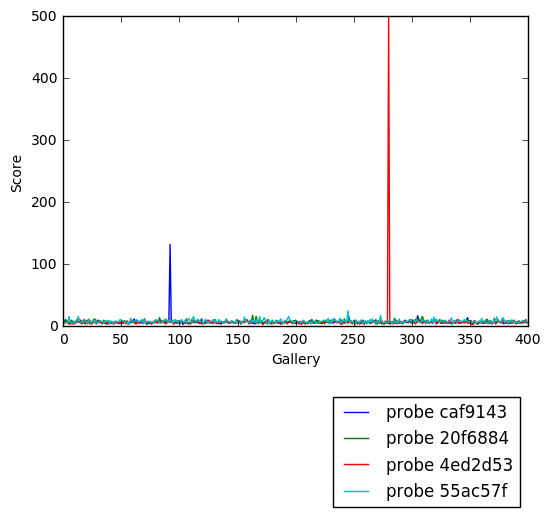
\includegraphics{fingerprint_matching_files/fingerprint_matching_74_0.png}

\begin{verbatim}
cursor.close()
\end{verbatim}



%----------------------------------------------------------------------------------------
%	LINUX
%----------------------------------------------------------------------------------------

\part{Linux}

\FILENAME

\section{Linux Shell}\label{linux-shell}

There are many good tutorials out there that explain why one needs a
linux shell and not just a GUI. Randomly we picked the firts one that
came up with a google query (This is not an endorsement for the material
we point to, but could be a worth while read for someone that has no
experience in Shell programming:

\begin{itemize}
\tightlist
\item
  \url{http://linuxcommand.org/lc3_learning_the_shell.php}
\end{itemize}

Certainly you are welcome to use other resources that may suite you
best. We will however summarize in table form a number of useful
commands that you may als find in a link to a RefCard.

\begin{itemize}
\tightlist
\item
  \url{http://www.cheat-sheets.org/\#Linux}
\end{itemize}

\subsection{File commands}\label{file-commands}

Find included a number of commands related to file manipulation.

\begin{longtable}[]{@{}ll@{}}
\toprule
\begin{minipage}[b]{0.26\columnwidth}\raggedright\strut
Command\strut
\end{minipage} & \begin{minipage}[b]{0.50\columnwidth}\raggedright\strut
Description\strut
\end{minipage}\tabularnewline
\midrule
\endhead
\begin{minipage}[t]{0.26\columnwidth}\raggedright\strut
ls\strut
\end{minipage} & \begin{minipage}[t]{0.50\columnwidth}\raggedright\strut
Directory listing\strut
\end{minipage}\tabularnewline
\begin{minipage}[t]{0.26\columnwidth}\raggedright\strut
ls -lisa\strut
\end{minipage} & \begin{minipage}[t]{0.50\columnwidth}\raggedright\strut
list details\strut
\end{minipage}\tabularnewline
\begin{minipage}[t]{0.26\columnwidth}\raggedright\strut
cd \emph{dirname}\strut
\end{minipage} & \begin{minipage}[t]{0.50\columnwidth}\raggedright\strut
Change directory to \emph{dirname}\strut
\end{minipage}\tabularnewline
\begin{minipage}[t]{0.26\columnwidth}\raggedright\strut
mkdir \emph{dirname}\strut
\end{minipage} & \begin{minipage}[t]{0.50\columnwidth}\raggedright\strut
create the directory\strut
\end{minipage}\tabularnewline
\begin{minipage}[t]{0.26\columnwidth}\raggedright\strut
pwd\strut
\end{minipage} & \begin{minipage}[t]{0.50\columnwidth}\raggedright\strut
print working directory\strut
\end{minipage}\tabularnewline
\begin{minipage}[t]{0.26\columnwidth}\raggedright\strut
rm \emph{file}\strut
\end{minipage} & \begin{minipage}[t]{0.50\columnwidth}\raggedright\strut
remove the file\strut
\end{minipage}\tabularnewline
\begin{minipage}[t]{0.26\columnwidth}\raggedright\strut
cp \emph{a} \emph{b}\strut
\end{minipage} & \begin{minipage}[t]{0.50\columnwidth}\raggedright\strut
copy file \emph{a} to \emph{b}\strut
\end{minipage}\tabularnewline
\begin{minipage}[t]{0.26\columnwidth}\raggedright\strut
mv \emph{a} \emph{b}\strut
\end{minipage} & \begin{minipage}[t]{0.50\columnwidth}\raggedright\strut
move/rename file \emph{a} to \emph{b}\strut
\end{minipage}\tabularnewline
\begin{minipage}[t]{0.26\columnwidth}\raggedright\strut
cat \emph{a}\strut
\end{minipage} & \begin{minipage}[t]{0.50\columnwidth}\raggedright\strut
print content of file\emph{a}\strut
\end{minipage}\tabularnewline
\begin{minipage}[t]{0.26\columnwidth}\raggedright\strut
less \emph{a}\strut
\end{minipage} & \begin{minipage}[t]{0.50\columnwidth}\raggedright\strut
print paged content of file \emph{a}\strut
\end{minipage}\tabularnewline
\begin{minipage}[t]{0.26\columnwidth}\raggedright\strut
head -5 \emph{a}\strut
\end{minipage} & \begin{minipage}[t]{0.50\columnwidth}\raggedright\strut
Display first 5 lines of file \emph{a}\strut
\end{minipage}\tabularnewline
\begin{minipage}[t]{0.26\columnwidth}\raggedright\strut
tail -5 \emph{a}\strut
\end{minipage} & \begin{minipage}[t]{0.50\columnwidth}\raggedright\strut
Display last 5 lines of file \emph{a}\strut
\end{minipage}\tabularnewline
\bottomrule
\end{longtable}

\subsection{Search commands}\label{search-commands}

Find included a number of commands related to seraching.

\begin{longtable}[]{@{}ll@{}}
\toprule
\begin{minipage}[b]{0.46\columnwidth}\raggedright\strut
Command\strut
\end{minipage} & \begin{minipage}[b]{0.21\columnwidth}\raggedright\strut
Description\strut
\end{minipage}\tabularnewline
\midrule
\endhead
\begin{minipage}[t]{0.46\columnwidth}\raggedright\strut
fgrep\strut
\end{minipage} & \begin{minipage}[t]{0.21\columnwidth}\raggedright\strut
TBD\strut
\end{minipage}\tabularnewline
\begin{minipage}[t]{0.46\columnwidth}\raggedright\strut
grep -R ``xyz'' .\strut
\end{minipage} & \begin{minipage}[t]{0.21\columnwidth}\raggedright\strut
TBD\strut
\end{minipage}\tabularnewline
\begin{minipage}[t]{0.48\columnwidth}\raggedright\strut
find . -name ``*.py'' \textbar{} TBD \textbar{}\strut
\end{minipage} & \begin{minipage}[t]{0.48\columnwidth}\raggedright\strut
\strut
\end{minipage}\tabularnewline
\bottomrule
\end{longtable}

\subsection{Help}\label{help}

Find included a number of commands related to manual pages.

\begin{longtable}[]{@{}ll@{}}
\toprule
\begin{minipage}[b]{0.24\columnwidth}\raggedright\strut
Command\strut
\end{minipage} & \begin{minipage}[b]{0.44\columnwidth}\raggedright\strut
Description\strut
\end{minipage}\tabularnewline
\midrule
\endhead
\begin{minipage}[t]{0.24\columnwidth}\raggedright\strut
man \emph{command}\strut
\end{minipage} & \begin{minipage}[t]{0.44\columnwidth}\raggedright\strut
manual page for the \emph{command}\strut
\end{minipage}\tabularnewline
\bottomrule
\end{longtable}

\subsection{Keyboard Shortcuts}\label{keyboard-shortcuts}

These shortcuts will come in handy. Note that many overlap with emacs
short cuts.

\begin{longtable}[]{@{}ll@{}}
\toprule
\begin{minipage}[b]{0.17\columnwidth}\raggedright\strut
Keys\strut
\end{minipage} & \begin{minipage}[b]{0.77\columnwidth}\raggedright\strut
Description\strut
\end{minipage}\tabularnewline
\midrule
\endhead
\begin{minipage}[t]{0.17\columnwidth}\raggedright\strut
Up Arrow\strut
\end{minipage} & \begin{minipage}[t]{0.77\columnwidth}\raggedright\strut
Show the previous command\strut
\end{minipage}\tabularnewline
\begin{minipage}[t]{0.17\columnwidth}\raggedright\strut
Ctrl + z\strut
\end{minipage} & \begin{minipage}[t]{0.77\columnwidth}\raggedright\strut
Stops the current command\strut
\end{minipage}\tabularnewline
\begin{minipage}[t]{0.48\columnwidth}\raggedright\strut
\strut
\end{minipage} & \begin{minipage}[t]{0.48\columnwidth}\raggedright\strut
resume with fg in the foreground\strut
\end{minipage}\tabularnewline
\begin{minipage}[t]{0.48\columnwidth}\raggedright\strut
\strut
\end{minipage} & \begin{minipage}[t]{0.48\columnwidth}\raggedright\strut
resume with bg in the background\strut
\end{minipage}\tabularnewline
\begin{minipage}[t]{0.17\columnwidth}\raggedright\strut
Ctrl + c\strut
\end{minipage} & \begin{minipage}[t]{0.77\columnwidth}\raggedright\strut
Halts the current command\strut
\end{minipage}\tabularnewline
\begin{minipage}[t]{0.17\columnwidth}\raggedright\strut
Ctrl + l\strut
\end{minipage} & \begin{minipage}[t]{0.77\columnwidth}\raggedright\strut
Clear the screen\strut
\end{minipage}\tabularnewline
\begin{minipage}[t]{0.17\columnwidth}\raggedright\strut
Ctrl + a\strut
\end{minipage} & \begin{minipage}[t]{0.77\columnwidth}\raggedright\strut
Return to the start of the command you're typing\strut
\end{minipage}\tabularnewline
\begin{minipage}[t]{0.17\columnwidth}\raggedright\strut
Ctrl + e\strut
\end{minipage} & \begin{minipage}[t]{0.77\columnwidth}\raggedright\strut
Go to the end of the command you're typing\strut
\end{minipage}\tabularnewline
\begin{minipage}[t]{0.17\columnwidth}\raggedright\strut
Ctrl + k\strut
\end{minipage} & \begin{minipage}[t]{0.77\columnwidth}\raggedright\strut
Cut everything after the cursor to a special clipboard\strut
\end{minipage}\tabularnewline
\begin{minipage}[t]{0.17\columnwidth}\raggedright\strut
Ctrl + y\strut
\end{minipage} & \begin{minipage}[t]{0.77\columnwidth}\raggedright\strut
Paste from the special clipboard\strut
\end{minipage}\tabularnewline
\begin{minipage}[t]{0.17\columnwidth}\raggedright\strut
Ctrl + d\strut
\end{minipage} & \begin{minipage}[t]{0.77\columnwidth}\raggedright\strut
Log out of current session, similar to exit\strut
\end{minipage}\tabularnewline
\bottomrule
\end{longtable}

\subsection{.bashrc and .bash\_profile}\label{bashrc-and-.bash_profile}

Usage of a particular command and all the attributes associated with it,
use `man' command. Avoid using `rm -r' command to delete files
recursively. A good way to avoid accidental deletion is to include the
following in your .bash\_profile file:

\begin{verbatim}
alias e=open_emacs
alias rm='rm -i'
alias mv='mv -i' 
alias h='history'
\end{verbatim}

More Information

\url{https://cloudmesh.github.io/classes/lesson/linux/refcards.html}

\subsection{Exercise}\label{exercise}

\begin{description}
\item[Linux.1:]
Familiarize yourself with the commands
\item[Linux.2:]
Find more commands that you find useful and add them to this page.
\item[Linux.3:]
Use the sort command to sort all lines of a file while removing
duplicates.
\end{description}

\begin{fileremark}\url{https://github.com/cloudmesh/classes/blob/master/docs/source/lesson/linux/virtualbox.rst}\end{fileremark}
\section{Virtual Box Installation and
Instructions}\label{virtual-box-installation-and-instructions}

For development purposes we recommend tha you use for this class an
ubuntu virtual machine that you set up with the help of virtualbox.

Only after you have successfully used ubuntu in a virtual machine you
will be allowed to use virtual machine son clouds.

A ``cloud drivers license test'' will be conducted to let you gain
access to the cloud infrastructure. We will announce this test. Before
you have not passed the test, you will not be able to use the clouds.
Furthermore, you do not have to ask us for join requests before you have
not passed the test. Please be patient. Only students enrolled in the
class can get access to the cloud.

\subsection{Creation}\label{creation}

First you will need to install virtualbox. It is easy to install and
details can be found at

\begin{itemize}
\tightlist
\item
  \url{https://www.virtualbox.org/wiki/Downloads}
\end{itemize}

After you have installed virtualbox you also need to use an image. For
this class we will be using ubuntu Desktop 16.04 which you can find at:

\begin{itemize}
\tightlist
\item
  \url{http://www.ubuntu.com/download/desktop}
\end{itemize}

Please note the recommended requirements that also apply to a virtual
machine:

\begin{itemize}
\tightlist
\item
  2 GHz dual core processor or better
\item
  2 GB system memory
\item
  25 GB of free hard drive space
\end{itemize}

A video to showcase such an install is available at:

\begin{itemize}
\tightlist
\item
  Video: \url{https://youtu.be/NWibDntN2M4}
\end{itemize}

\begin{description}
\item[If you specify your machien too small you will not be]
able to install the development environment. Gregor used on his machine
8gb of RAM and 20GB diskspace.
\end{description}

Please let us know the smalest configuration that works for you and
share this in Piaza. Only update if yours is smaller and works than a
previous post. If not do not post.

\subsection{Guest additions}\label{guest-additions}

The virtual guest additions allow you to easily do the following tasks:

\begin{itemize}
\tightlist
\item
  Resize the windows of the vm
\item
  Copy and paste content between the Guest operating system and the host
  operating system windows.
\end{itemize}

This way you can use many native programs on you host and copy contents
easily into for example a terminal or an editor that you run in the Vm.

A video is located at

\begin{itemize}
\tightlist
\item
  Video: \url{https://youtu.be/wdCoiNdn2jA}
\end{itemize}

Please reboot the machine after installation and configuration.

On OSX you can once you have enabled bidirectional copying in the Device
tab with

\begin{description}
\item[OSX -\textgreater{} Vbox:]
command c -\textgreater{} shift CONTRL v
\item[Vbox to OSX:]
shift CONTRL v -\textgreater{} shift CONTRL v
\end{description}

On Windows the key combination is naturally different. Please consult
your windows manual.

\subsection{Exercise}\label{exercise}

\begin{description}
\item[Virtualbox.1:]
Install ubuntu desktop on your computer with guest additions.
\item[Virtualbox.2:]
Make sure you know how to paste and copy between your host and guest
operating system
\item[Virtualbox.3:]
Install the programs defined by the development configuration
\end{description}



%----------------------------------------------------------------------------------------
%	PART
%----------------------------------------------------------------------------------------

\part{IoT}

%----------------------------------------------------------------------------------------
%	CHAPTER 1
%----------------------------------------------------------------------------------------

\chapterimage{chapter_head_2.png} % Chapter heading image

\begin{fileremark}\url{https://github.com/cloudmesh/classes/blob/master/docs/source/lesson/iot/introduction.md}\end{fileremark}
\section{Introduction}\label{introduction}

Internet of Things is one of the driving forces in the modernisation of
todays world. It is based on connecting \emph{things} to the internet to
create a more aware world that can be interfaced with. This not only
includes us humans, but any \emph{thing} that can interact with other
things. It is clear that such a vision of interconnected devices will
result in billions of devices to communicate with each other. Some of
them may only communicate small number of items, while others will
communicate a large amount. Analysis of this data is dependent on the
capability of the \emph{thing}. If it is to small the analysis can be
conducted on a remote server or cloud while information to act are fead
back from the device. In other cases the device may be completely
autonomous and does not require any interaction. Yet in other cases the
collaborative information gathered from such devices is used to derive
decissions and actions.

Within this section we are trying to provide you with a small glimpse
into how IoT devices function and can be utilized on small projects.
Ideally if the class has all such a device we could even attempt to
build a cloud based service that collects and redistributes the data.

To keep things simple we are not providing a general introduction in
IoT. For that we offer other classes. However, we will introduce you to
two different devices. These are

\begin{itemize}
\tightlist
\item
  esp8266
\item
  Raspberry Pi
\end{itemize}

The reasons we chose them is that

\begin{enumerate}
\def\labelenumi{\arabic{enumi}.}
\tightlist
\item
  they are cheap,
\item
  we can program both in python allowing us to use a single programming
  langauage for all projects and assignments, and
\item
  they are sufficiently powerful and we can conduct real projects with
  them beyond toy projects.
\item
  the devices, especially the Raspberry PI can be used to also learn
  Linux in case you do not have access to a linux computer. Please note
  however the raspberry will have memory and space limitations that you
  need to deal with.
\end{enumerate}

Projects that you can do to test the devices are

esp8266 (easy-moderate, small memory):

\begin{enumerate}
\def\labelenumi{\arabic{enumi}.}
\tightlist
\item
  a LED blinker
\item
  a dendrite
\item
  a robot fish
\item
  a fish swarm
\item
  a robot swarm
\item
  an activity of your desire
\end{enumerate}

Raspberry Pi (easy-moderate, 32GB space limitation):

\begin{enumerate}
\def\labelenumi{\arabic{enumi}.}
\tightlist
\item
  a LED blinker
\item
  a robot car
\item
  a robot car with camera
\item
  a termerature service
\item
  a docker cluster
\end{enumerate}

Crazyflie 2.0 (difficult):

\begin{enumerate}
\def\labelenumi{\arabic{enumi}.}
\tightlist
\item
  programming a drone
\item
  programming a drone swarm
\end{enumerate}

Please note that for those at IU we do have a Lab in which you can use
some of the devices pointed out here. You can arrange for accessing the
infrastructure or you simply can buy it for yourself.

We have a hardware page that summarizes what you need. In case you want
to work on a swarm, we do have positioning sensors that simplify that
task.

In general we think that these platforms provide a wonderful
introduction into IoT and where it will move to. Such platforms were
just a decade ago not powerful enough or too expensive. However today
the provide a serious platform for developers. Sensors are available
easily as most Android comparible sensors can be used.

Before we jump right into programming the devices, we like to point out
that we dod not chose to use Arduinos, as their price advantage is no
longer valid. We also find that esp8266 and Raspberry can interface with
most sensors. Having the ability to easily use WiFi however is our
primary reason for using them. Furthermore being able to attach a camera
to the Raspberry is just superb. Image analysis will be one of the near
term future drivers for big data.

\FILENAME

\section{Hardware for IoT Projects}\label{hardware-for-iot-projects}

When teaching programming you may find yourself in a situation that
things can be done on your computer, but you may not want to install
programs that help you to learn programming on your computer. However,
we have a solution (or several) for you. We will have some fun with
hardware for IoT that at the same time can be used to teach you some
very elementary skills in programming. However, if you would rather use
your computer you certainly can do this too.

We see the following arguments for using IoT hardware:

\begin{itemize}
\tightlist
\item
  You will have fun with inexpensive hardware
\item
  You will get hands on experience with IOT devices
\item
  You will learn how to program in python
\item
  You can keep your current computer unchanged
\item
  You will get experience with two platforms esp8266 and Raspberry PI 3
\item
  You can customise your choices by conducting some fun projects.
\item
  You have the opportunity to find alternative hardware choices such as
  the WiPy or the ESP32. You may find cheaper or better alternatives if
  you buy kits when they are available. And learn in getting an overview
  about such devices and kits.
\end{itemize}

\emph{Note:} Ordering from overseas suppliers may take significant time,
so make sure to plan ahead. Prices given here are done to provide an
estimate, they may vary.

\subsection{Raspberry Pi 3}\label{raspberry-pi-3}

The raspberry PI 3 is a very good development platform. With its base
price of \$35 it is quite a bargain. You will need some additional
components to make sure you can use it. Please be reminded to never
connect or power the raspberry with your computers USB port. It draws
some significant amperage and we do not want you to destroy your
computer. We recommend that you buy a certified power adapter. The price
is so cheap that you could even create your own mini cluster as a
project. We do not recommend any older versions of Raspberry as they are
less powerful and do not contain built-in Bluetooth or WiFi.

\emph{Configuration:}

\begin{itemize}
\tightlist
\item
  \$37.50
  \href{https://www.amazon.com/Raspberry-Model-A1-2GHz-64-bit-quad-core/dp/B01CD5VC92/ref=sr_1_1?s=pc\&ie=UTF8\&qid=1499251061\&sr=1-1\&keywords=raspberry+pi+3}{Pi
  3}
\item
  \$7.69
  \href{https://www.amazon.com/Eleduino-Raspberry-Model-Acrylic-Enclosure/dp/B01CQRROLW/ref=sr_1_7?s=electronics\&ie=UTF8\&qid=1499251106\&sr=1-7\&keywords=raspberry+pi+3+case}{Case}
\item
  \$7.99
  \href{https://www.amazon.com/Enokay-Supply-Raspberry-Charger-Adapter/dp/B01MZX466R/ref=sr_1_3?ie=UTF8\&qid=1498443576\&sr=8-3\&keywords=raspberry+pi+power+adapter+micro+usb+switch}{Power
  Adapter} This is an aftermarket poweradapter. Lots uof us use this
  one.
\item
  \$6.99
  \href{https://www.amazon.com/AmazonBasics-High-Speed-HDMI-Cable-Standard/dp/B014I8SSD0/ref=sr_1_3?ie=UTF8\&qid=1499253502\&sr=8-3\&keywords=hdmi+cable}{HDMI
  cable}
\item
  Monitor/TV with hdmi
\item
  SD Card, 8GB minimum, 32GB maximum
\end{itemize}

\emph{Advantages:}

\begin{itemize}
\tightlist
\item
  Full Linux like OS based on debian
\item
  Good environment for learning Linux and Python
\item
  Reasonable interfaces to IoT sensors
\item
  excellent camera support
\item
  excellent choice of expansion packages including Grove Sensors that
  make it easy to attach sensors and actuators. An example package is
  the
  \href{https://www.amazon.com/GrovePi-Starter-Kit-Dexter-Industries/dp/B00TXTZ5SQ/ref=pd_lpo_vtph_147_bs_tr_img_1?_encoding=UTF8\&psc=1\&refRID=45QX6XSNZAG1NT8NES79}{Grove
  Starter Kit} for about \$90
\end{itemize}

\emph{Disadvantages:}

\begin{itemize}
\tightlist
\item
  We tried the Windows IoT package and were not impressed by it. This is
  not an issue of the Raspberry, but the Windows IoT platform
\end{itemize}

\subsection{ESP8266 Robot Car Kit}\label{esp8266-robot-car-kit}

The ESP8266 has many variants. Some of which are difficult to interface
with. However, this does not apply for the ESP8266 NodeMCU. This board
is originally flashed with \emph{Lua}, however it can easily be
reflashed with MicroPython. In addition it is often offered as part of a
platform to develop a robot car. There are arguably better kits
available, but the price of \$24 for the entire kit is hard to beat.
Unfortunately the version of python, as well as the limited memory make
the esp8266 not a full fledged platform for python programming and you
will quickly see its limitations. Interfacing with it, however, as an
IoT device will gain you a lot of insights.

\emph{Configuration:}

\begin{itemize}
\tightlist
\item
  \$14.99
  \href{https://www.amazon.com/KOOKYE-ESP8266-NodeMcu-ESP-12E-Expansion/dp/B01C6MR62E/ref=sr_1_1?ie=UTF8\&qid=1499251895\&sr=8-1\&keywords=esp8266+robot+car}{esp8266
  \& shield} or
  \href{https://www.amazon.com/Makerfocus-ESP8266-ESP-12E-Development-Expansion/dp/B01MU4XQUN/ref=sr_1_2?ie=UTF8\&qid=1499252002\&sr=8-2\&keywords=esp8266+motor+shield}{esp8266
  \& shield}
\item
  \$12.59
  \href{https://www.amazon.com/Emgreat-Chassis-Encoder-wheels-Battery/dp/B00GLO5SMY/ref=pd_rhf_se_s_cp_10?_encoding=UTF8\&pd_rd_i=B00GLO5SMY\&pd_rd_r=77XYGK6BE54FGDTGQ0AC\&pd_rd_w=FNQFl\&pd_rd_wg=wKMdb\&psc=1\&refRID=77XYGK6BE54FGDTGQ0AC}{Chasis}
\item
  4 * AA Rechargable Batteries \& charger
\end{itemize}

Optionally you may want to get additional sensors such as wheel Encoders

\begin{itemize}
\tightlist
\item
  \href{https://www.amazon.com/Wheel-Encoder-Kit-Robot-Car/dp/B00NPWGEIM/ref=sr_1_4?s=toys-and-games\&ie=UTF8\&qid=1499254488\&sr=1-4\&keywords=speed+sensor+robot+car+wheel}{Wheel
  Encoder}
\end{itemize}

\emph{Advantages:}

\begin{itemize}
\item
  Very low price for what it can do
\item
  We have OSX software available that makes it easy to setup (Other
  tutorials for other platforms are available on the internet, you can
  contribute by creating documentation we distribute in class for
  points)
\item
\item
\end{itemize}

\subsection{Sensor Kit}\label{sensor-kit}

It is fun to attach sensors to your IoT board. There are many kits
ab{]}vailable and we encourage you to do comparisions. One such kit is

\begin{itemize}
\tightlist
\item
  \$29.99
  \href{https://www.amazon.com/Elegoo-Upgraded-Modules-Tutorial-Arduino/dp/B01MG49ZQ5/ref=sr_1_7?s=electronics\&ie=UTF8\&qid=1499251441\&sr=1-7\&keywords=elegoo}{Elegoo
  37 Sensors}
\end{itemize}

However it does not include a breadboard like other kits. Hence we
recommend that you get a breadboard as it makes experimenting easier.

\begin{itemize}
\tightlist
\item
  \$5.68
  \href{https://www.amazon.com/Elegoo-Premium-Female-tie-points-breadboard/dp/B06XB8TZVC/ref=sr_1_23?s=electronics\&ie=UTF8\&qid=1499251600\&sr=1-23\&keywords=elegoo}{small
  bread board and wires}
\end{itemize}

\subsection{Fish Kit}\label{fish-kit}

\begin{itemize}
\tightlist
\item
  \$29.99
  \href{https://www.amazon.com/Swimmer-Inflatable-Flying-Replacement-Balloon/dp/B00658LN3E/ref=pd_bxgy_21_img_2?_encoding=UTF8\&pd_rd_i=B00658LN3E\&pd_rd_r=F71N2YCYE6Z0BCCEPQJC\&pd_rd_w=AwYab\&pd_rd_wg=rHTnv\&psc=1\&refRID=F71N2YCYE6Z0BCCEPQJC}{shark}

  \begin{itemize}
  \tightlist
  \item
    cheaper balloons leak
  \item
    before assembly and putting gas in, make sure components work.
  \item
    gas will last typically for one week
  \item
    \$39.99 gas can be purchased in party store
  \end{itemize}
\item
  2 g9 servo
\item
  soldering (for cable, so cheap one will do)
\item
  pins
\item
  esp
\item
  double sided scotch tape
\item
  hot glue gun
\item
  paper clips
\end{itemize}

\subsection{Alternative components}\label{alternative-components}

\subsubsection{Esp8266 Alternatives}\label{esp8266-alternatives}

Two models are good. Adafruit has some added features, but may need
soldering

\begin{itemize}
\tightlist
\item
  \$8.79
  \href{https://www.amazon.com/HiLetgo-Version-NodeMCU-Internet-Development/dp/B010O1G1ES/ref=sr_1_3?s=electronics\&ie=UTF8\&qid=1499251149\&sr=1-3\&keywords=esp8266}{NodeMCU}
\item
  \$16.95 \href{https://www.adafruit.com/product/2821}{Adafruit Feather}
\end{itemize}

\subsubsection{Car Parts Alternatives}\label{car-parts-alternatives}

\begin{itemize}
\tightlist
\item
  \$14.59
  \href{https://www.amazon.com/Ardokit-Chassis-Encoder-Battery-Arduino/dp/B00K5OWHXO/ref=sr_1_3?s=electronics\&ie=UTF8\&qid=1499251712\&sr=1-3\&keywords=robot+car}{Car
  Chasis}
\item
  \$22.88
  \href{https://www.amazon.com/VKmaker-Avoidance-tracking-Chassis-Ultrasonic/dp/B01CXVA6IO/ref=sr_1_6?s=electronics\&ie=UTF8\&qid=1499251770\&sr=1-6\&keywords=robot+car}{Car
  Chasis and Arduino}
\end{itemize}

\subsubsection{Simple sensors}\label{simple-sensors}

Simple sensors can be attached to the boards with cables (that you need
to purchase separately). Examples include

\begin{itemize}
\tightlist
\item
  \href{https://www.amazon.com/Elegoo-Sensor-Module-Arduino-MEGA/dp/B009OVGKTQ/ref=sr_1_5?s=electronics\&ie=UTF8\&qid=1500678010\&sr=1-5\&keywords=grove+sensor}{Elegoo
  37 sensor kit}
\item
  \href{https://www.amazon.com/Breadboard-Wires-Aoyoho-Multicolored-Jumper/dp/B01GK2Q4ZQ/ref=sr_1_1?s=electronics\&ie=UTF8\&qid=1500678142\&sr=1-1\&keywords=bread+board+cab\%3Be}{Breadboard
  Cable}
\end{itemize}

\subsubsection{Grove Sensors}\label{grove-sensors}

Grove sensors have ready-made cables that make them easy to attach to
the Raspberry PI. However, they are more expensive. You still need a
Raspberry PI. No soldering iron and no breadboards are required.

\begin{itemize}
\tightlist
\item
  \href{https://www.seeedstudio.com/Grove-Starter-Kit-for-Arduino-p-1855.html}{Grove
  Starter Set}
\item
  \href{https://www.seeedstudio.com/category/Grove-c-1003.html}{Seed
  Studio Grove Sensors}
\item
  \href{https://www.seeedstudio.com/Grove-Base-Shield-for-NodeMCU-p-2513.html}{Grove
  Shield for NodeMCU}
\item
  \href{http://www.switchdoc.com/2016/02/tutorial-intro-to-grove-connectors-for-arduinoraspberry-pi-projects/}{Grove
  Cable}
\end{itemize}

\FILENAME

\section{Projects}\label{projects}

Please see the introduction to the IoT section to get started.

Term project suggestion combining IoT and Big Data:

\begin{enumerate}
\def\labelenumi{\arabic{enumi}.}
\tightlist
\item
  Recognizing street sign in a car robot with a camera
\item
  Regognizing street lines in a car robot with camera
\item
  Driving a Robot car swarm without collisions
\item
  Simulating a City with robot cars
\item
  Control a robot fish with cameras
\item
  Build a distributed sensor system (with your classmates)
\end{enumerate}

Drones:

\begin{enumerate}
\def\labelenumi{\arabic{enumi}.}
\tightlist
\item
  Control a drone swarm with positioning system
\end{enumerate}

Suggest your own

\begin{fileremark}\url{https://github.com/cloudmesh/classes/blob/master/docs/source/lesson/iot/esp8266/esp8266.md}\end{fileremark}
\section{ESP8266}\label{esp8266}

When working with a external hardware such as the NodeMCU you will find
a lot of information on the internet about it. It is a bit difficult at
times to assess what you need to program it. You are exposed to many
choices. A NodeMCU typically comes with Lua. However you have many other
choices. Such choices include multiple programming languages such as
Lua, MicroPython, Arduino/C, Go and others.

As all of them are slightly different you need to identify which works
best for you. In addition you need to install images, programs and
libraries that support your specific language choice.

For our first experiments we will be using MicroPython. This choice is
motivated by the fact that Python is a well established and easy to
learn programming language. Recently many educational institutions are
offering Python as an introductory programming language making this
choice even mor compelling

To simplify the setup and use of the esp8266 for MicroPython we
developed an easy to use commandline tool that allows users to set up
their computer and interact more easily with the board. We believe that
the interface is so simple that it can also be used in STEM activities
and not just in the university or by advanced hobbyists.

\subsection{Installation}\label{installation}

In this section we discuss the various ways on how to set up the esp8266
\texttt{cloudmesh.robot} development environment. You have several
options to install it.

\begin{enumerate}
\def\labelenumi{\arabic{enumi}.}
\tightlist
\item
  Option A: OSX with scripts hosted on github (recommended)
\item
  Option B: OSX from source
\item
  OPtion C: Explore your own
\end{enumerate}

While we provide here a detailed option for OSX, you are free to explore
other operating systems. We know that it can for example be installed on
Ubuntu 16.04. We have not tested any of this on a Windows machine.

We like to get feedback and instalation instructions.

\subsubsection{Option A: OSX install from a
Script}\label{option-a-osx-install-from-a-script}

For OSX we have created two scripts that you will need

\begin{itemize}
\tightlist
\item
  \href{http://cloudmesh.github.io/get/robot/osx/system/}{system.sh},
  that installs pip, ansible, homebrew, xcode, virtualenv, readline,
  wget, lua, picocom, mosquito, aquaemacs, pycharm, numpy, matplotlib,
  libusb, USB drivers for selkected esp8266 (ch34x chip)
\item
  \href{http://cloudmesh.github.io/get/robot/osx/user}{user.sh}, that
  installs matplotlib, virtualenv, and the cloudmesh source in
  \textasciitilde{}/github
\end{itemize}

We recommend that you review these scripts carfully before you use them
and check if they fit your needs. If they do not, please just download t
hem and adapt them to your needs. The \textbf{system} script must be ran
on an \textbf{Administrator} account as it requires sudo priviledges.
The \textbf{user} script must be ran on a \textbf{User} account. We do
not recommend to run the IoT software in an administrative account due
to security best practices. To execute the \textbf{system} script, type
in the \emph{Administrator account} terminal

\begin{verbatim}
curl -fsSL http://cloudmesh.github.io/get/robot/osx/system | sh
    
\end{verbatim}

As earlier versions of pip may have some issues, this script will also
update pip and setuptools to a neweer version

To execute the \textbf{user} script, type in the User account terminal

\begin{verbatim}
 curl -fsSL http://cloudmesh.github.io/get/robot/osx/user | sh
\end{verbatim}

Together these scripts allow you to install in a simple way development
tools for our IoT activities.

The following steps are to be executed in the user environment.

\textbf{Warning}: \emph{the scripts do not update pip and setuptool,
which may be required due to a bug in setuptools prior to version 34 for
setuptools. You may have to repeat the update on any pyenv environment
that you use. How to do thi sis documented in a later section.}

To simplify use, we recommend that you make the following additions to
your \texttt{\textasciitilde{}/.bash\_profile} file so that python 3 is
automatically activated, but does not interfere with the system
installed python. Use the command

\begin{verbatim}
$ emacs ~/.bash_profile
\end{verbatim}

or your favourite editor to edit the file and add the following lines at
the end.

\begin{verbatim}
####################################################################### 
# PYENV
######################################################################
open_emacs() {
    # open -na Aquamacs $*
    open -a Aquamacs $*    
}
alias e=open_emacs

########################################################
# PYENV
########################################################
export PYENV_VIRTUALENV_DISABLE_PROMPT=0
eval "$(pyenv init -)"
eval "$(pyenv virtualenv-init -)"
__pyenv_version_ps1() {
    local ret=$?;
    output=$(pyenv version-name)
    if [[ ! -z $output ]]; then
    echo -n "($output)"
    fi
    return $ret;
}
PS1="\$(__pyenv_version_ps1) ${PS1}"   
alias ENV3="pyenv activate ENV3"
ENV3
\end{verbatim}

Once you start a new terminal you can edit files via aquaemacs by typing

\begin{verbatim}
e FILENAME
\end{verbatim}

where FILENAME is the name of the file you like to edit. However the
file must exists, which you can simply do with

\begin{verbatim}
touch FILENAME
\end{verbatim}

Add the following lines at the end of the file

To learn more about how to you automate the setup of an OSX machine, you
may be inspired by

\begin{itemize}
\tightlist
\item
  \url{https://github.com/ricbra/dotfiles/blob/master/bin/setup_osx}
\item
  \url{https://blog.vandenbrand.org/2016/01/04/how-to-automate-your-mac-os-x-setup-with-ansible/}
\end{itemize}

\subsubsection{Setting Up Git}\label{setting-up-git}

Sooner or later you will be using git. We recommend that you set your
identity on all computers that you will be using. To do this adapt the
following example according to your github.com identity that you have.
IF you do not, its time to greate one at github.com and follow the
directions.

\begin{verbatim}
$ git config --global user.name "Gregor von Laszewski"
$ git config --global user.email laszewski@gmail.com
$ git config --global core.editor emacs
$ git config --global push.default matching
\end{verbatim}

\subsection{Option B: setup from pip}\label{option-b-setup-from-pip}

We have removed the pip setup instructions as they do not include
installing the drivers.

\subsubsection{Option B: Install Cloudmesh Robot from
source}\label{option-b-install-cloudmesh-robot-from-source}

Developers that already have a development environment (e.g.~xcode is
installed) can install cloudmesh robot also from the terminal while
downloading the source. You will need to first obtain the source and
compile it with the following commands:

\begin{verbatim}
$ mkdir github
$ cd github
$ git clone https://github.com/cloudmesh/cloudmesh.common.git
$ git clone https://github.com/cloudmesh/cloudmesh.cmd5.git
$ git clone https://github.com/cloudmesh/cloudmesh.robot.git
$ cd cloudmesh.robot
$ make source
\end{verbatim}

To test out if the command has been installed, type

\begin{verbatim}
$ cms robot welcome
\end{verbatim}

If everything works you should see an ASCII image of R2D2 and C3PO.
Next, we still have to install some additional programs before you can
use other commands.

Once you have installed cloudmesh robots you well be able to install a
number of tools automatically with the command

\begin{verbatim}
$ cms robot osx install
\end{verbatim}

This will install services and tools including xcode, homebrew, macdown,
pycharm, and aquaemacs. If you have some these tools already installed
it will skip the instalation process for a particular tool. Please note
that some of the tools require root access and thus you must be able to
have ccess to sudo to run them from our tool. In addition you will need
to install the OSX driver for the USB interface to the esp8266. This is
achieved with (only to be done if you follow the install from source
option)

\begin{verbatim}
$ cms robot osx driver
\end{verbatim}

Now please change your account to be again a standard account.

Now you \textbf{MUST REBOOT} the machine. Without rebooting you will not
be able to use the USB drivers.

\subsection{Option C: A possible setup for
Linux}\label{option-c-a-possible-setup-for-linux}

On a linux computer we recommend that you install emacs, cmake and
configure your git. Replace the user name and e-mail with the once that
you used to register your account in git:

\begin{verbatim}
$ mkdir github
$ cd github
$ git clone https://github.com/cloudmesh/cloudmesh.robot.git
$ ssh-keygen
$ sudo apt-get install -y emacs
$ sudo apt-get install -y cmake
$ sudo apt-get install -y libqt4-dev
$ git config --global user.name "Gregor von Laszewski"
$ git config --global user.email laszewski@gmail.com
$ git config --global core.editor emacs
$ git config --global push.default matching
\end{verbatim}

This setup is highly incomplete and does not include the setup of the
USB drivers. Please help us completing the documentation.

\subsubsection{Option C: A possible setup for
Windows}\label{option-c-a-possible-setup-for-windows}

We do not have tried to set this up on Windows or a virtualbox running
Linux under windows. If you have tried it, please let us know. If you
have difficulties just use a raspberry PI and skip the IoT projects

\subsubsection{Option C: Installation of the cloudmesh.robot Interface
via
Pip}\label{option-c-installation-of-the-cloudmesh.robot-interface-via-pip}

.. warning:: this option does not include installing the USB drivers.
You have to install them first. See examples on how to do that in our
install scripts. Generally what we do in our user.sh script is the same
way, but also includes the setup of python 3.6.1.

To more easily interface with the robot we have developed a convenient
program that is installed as part of a command tool called cloudmesh.

\subsubsection{Install Cloudmesh Robot with Pip (not
working)}\label{install-cloudmesh-robot-with-pip-not-working}

Note that pip may not include the newest version of cloudmesh.robot and
we recommend you use the source install instead.

\begin{verbatim}
$ pip install cloudmesh.robot 
\end{verbatim}

This will install a program \texttt{cms} on your computer that allows
you to easily communicate with the robot.

\subsection{Using cloudmesh robot}\label{using-cloudmesh-robot}

Once you have successfully installed the drivers and the commands you
can look at the manual page of the robot command with

\begin{verbatim}
$ cms robot help
\end{verbatim}

You will see a manual page like this:

\begin{verbatim}
Usage:
   robot welcome
   robot osx install
   robot osx driver
   robot image fetch
   robot probe [--format=FORMAT]
   robot flash erase [--dryrun]
   robot flash python [--dryrun]
   robot test
   robot run PROGRAM
   robot credentials set SSID USERNAME PASSWORD
   robot credentials put
   robot credentials list
   robot login
   robot set PORT NOT IMPLEMENTED
   robot ls [PATH]
   robot put [-o] SOURCE [DESTINATION]
   robot get PATH
   robot rm PATH
   robot rmdir PATH
   robot dance FILE IPS
   robot inventory list [--cat] [--path=PATH] [ID]
\end{verbatim}

\subsubsection{Testing the board}\label{testing-the-board}

Before you can use you ESP8266, you must have the appropriate drivers
installed on your computer. Click on
\href{https://github.com/cloudmesh/cloudmesh.robot/blob/7859b395fd15e4d6ced679b05893c9a91957c956/documentation/source/espdrivers.md}{this
link} and follow the instructions on how to install these drivers.

Next is to connect a esp8266 with a USB cable to the computer. The
ESP8266 should look similar to this.

After you connected it, press the reset button. Before doing anything on
the board, we must test it. Once you have plugged it in, execute the
following command:

\begin{verbatim}
$ cms robot probe
\end{verbatim}

This command takes about ten seconds to execute. The ESP8266's led
should flash irregularly as it is probed. When the probe is finished, an
image similar to the following should appear in your terminal:

\begin{verbatim}
+-----------+---------------------------+
| Attribute | Value                     |
+-----------+---------------------------+
| chipid    | b' 0x00d0f9ec'            |
| mac       | b' 00:10:FA:6E:38:4A'     |
| tty       | /dev/tty.wchusbserial1410 |
+-----------+---------------------------+
\end{verbatim}

Please note that you should only have one board attached to your
computer.

\subsubsection{Flashing the image onto the robot
board}\label{flashing-the-image-onto-the-robot-board}

Next we need to flash the image on the robot board. Naturally we need to
fetch the image first from the internet. We do this with the command

\begin{verbatim}
$ cms robot image fetch
\end{verbatim}

This will fetch an image that contains MicroPython into your local
directory.

Next we need to \emph{flash} the image on the board.

Before you begin, make sure that the ESP8266 is connected to your
computer. The board may come with a preinstalled image such as Lua or
some custom image from the vendor. In order to write programs in python,
we need to the chips to run micropython. To get micropython on our
ESP8266's, a number of steps are required.

\subsubsection{Erase the chip}\label{erase-the-chip}

First we need to erase the chip.

Run the following command in your terminal terminal, and then
\textbf{stop.}

\begin{verbatim}
$ cms robot flash erase
\end{verbatim}

Your terminal should respond with the following query:

\begin{verbatim}
/dev/tty.SLAB_USBtoUART
Please press the right buttons
continue? (Y/n)
\end{verbatim}

Before taking any further steps, press both buttons on the ESP8266 at
the same time. Once you have done this, type \texttt{Y} and press
\texttt{enter}. The process should take under ten seconds to complete.

\subsubsection{Putting Python on the
chip}\label{putting-python-on-the-chip}

Before proceeding, you must once again press both of the buttons on the
ESP8266. Once this is done, you are ready to flash the chip with python
with the following command:

\begin{verbatim}
$ cms robot flash python 
\end{verbatim}

\subsubsection{Testing if it works}\label{testing-if-it-works}

To test running a pyton program execute

\begin{verbatim}
$ cms robot test
\end{verbatim}

Be careful as it overwrites the file \texttt{test.py}. If the ESP8266 is
set up properly, it should return this in your terminal:

\begin{verbatim}
Count to 3
1
2
3
\end{verbatim}

\subsubsection{Execute an arbitrary
program}\label{execute-an-arbitrary-program}

Lets assume you have placed a program in the file \texttt{prg.py} with
the command

\begin{verbatim}
$ cms robot put prg.py  
\end{verbatim}

You must reboot the ESP8266 before using a new program. This can be done
manually by pressing the reset button on the chip, or in terminal with
the command

\begin{verbatim}
$ cms robot reset
\end{verbatim}

Once the chip is reset, you can run \texttt{prg.py} with the following
command:

\begin{verbatim}
$ cms robot run prg.py
\end{verbatim}

\subsubsection{Interactive Python shell on the
board}\label{interactive-python-shell-on-the-board}

To get into the interactive python shell on the board you need to reset
the ESP8266 and run the following command:

\begin{verbatim}
$ cms robot login
\end{verbatim}

\subsubsection{Cleaning an reinstalling a development
version}\label{cleaning-an-reinstalling-a-development-version}

IN case you are a developer and you need to modify the source code, we
found that it is sometimes necessary to clean your development directory
and libraries. The easiest way to do this is to go to the repository
that you like to reinstall. Let us assume it is \emph{cloudmesh.robot}.
Than the following commands will clean the repository

\begin{verbatim}
$ cd cloudmesh.robot
$ pip uninstall cloudmesh.robot
\end{verbatim}

Do the pip unisntall as many times till you see an error that no more
cloudmesh.robot versions can be found. Than execute

\begin{verbatim}
$ make clean
\end{verbatim}

After this you can reinstall it with

\begin{verbatim}
$ python setup.py install; pip install -e .
\end{verbatim}

the -e flag is optional, but allows you to change the code without the
need of recompiling. A very useful feature in python.

\subsubsection{NodeMCU ESP12 Dev Kit Pin
Definition}\label{nodemcu-esp12-dev-kit-pin-definition}

For V1.0

\begin{figure}
\centering
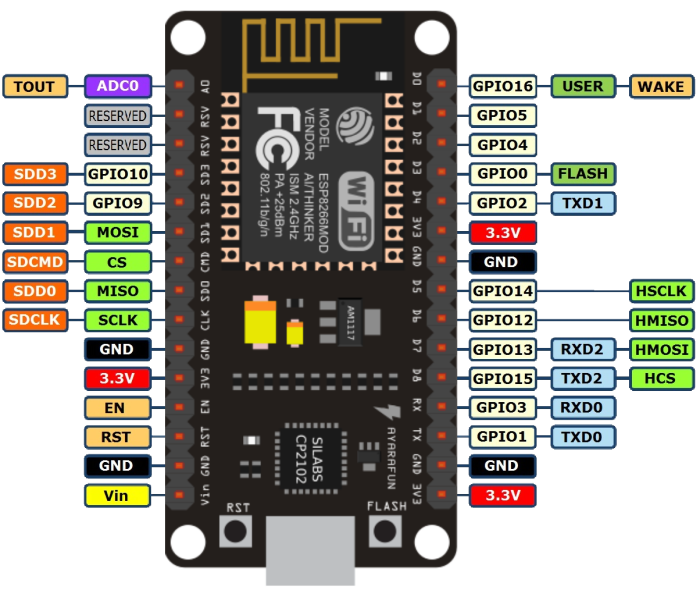
\includegraphics{../images/nodemcu.png}
\caption{nodemcs}
\end{figure}

The GPIO numbers of teh NodeMCU, do not correspond with the actual
numbers used in micropythons pin library. The numbers are as follows:

\begin{longtable}[]{@{}ll@{}}
\toprule
Pin/GPIO & NodeMCU\tabularnewline
\midrule
\endhead
15 & D8\tabularnewline
\bottomrule
\end{longtable}

\subsubsection{LED}\label{led}

\paragraph{Program}\label{program}

\begin{verbatim}
import machine
led = machine.Pin(15,machine.Pin.OUT)
led.high()
led.low()


import machine
led = machine.Pin(15,machine.Pin.OUT)
while True:
    led.high()
    time.sleep(0.5)
    led.low()
    time.sleep(0.5)
\end{verbatim}

\begin{figure}
\centering
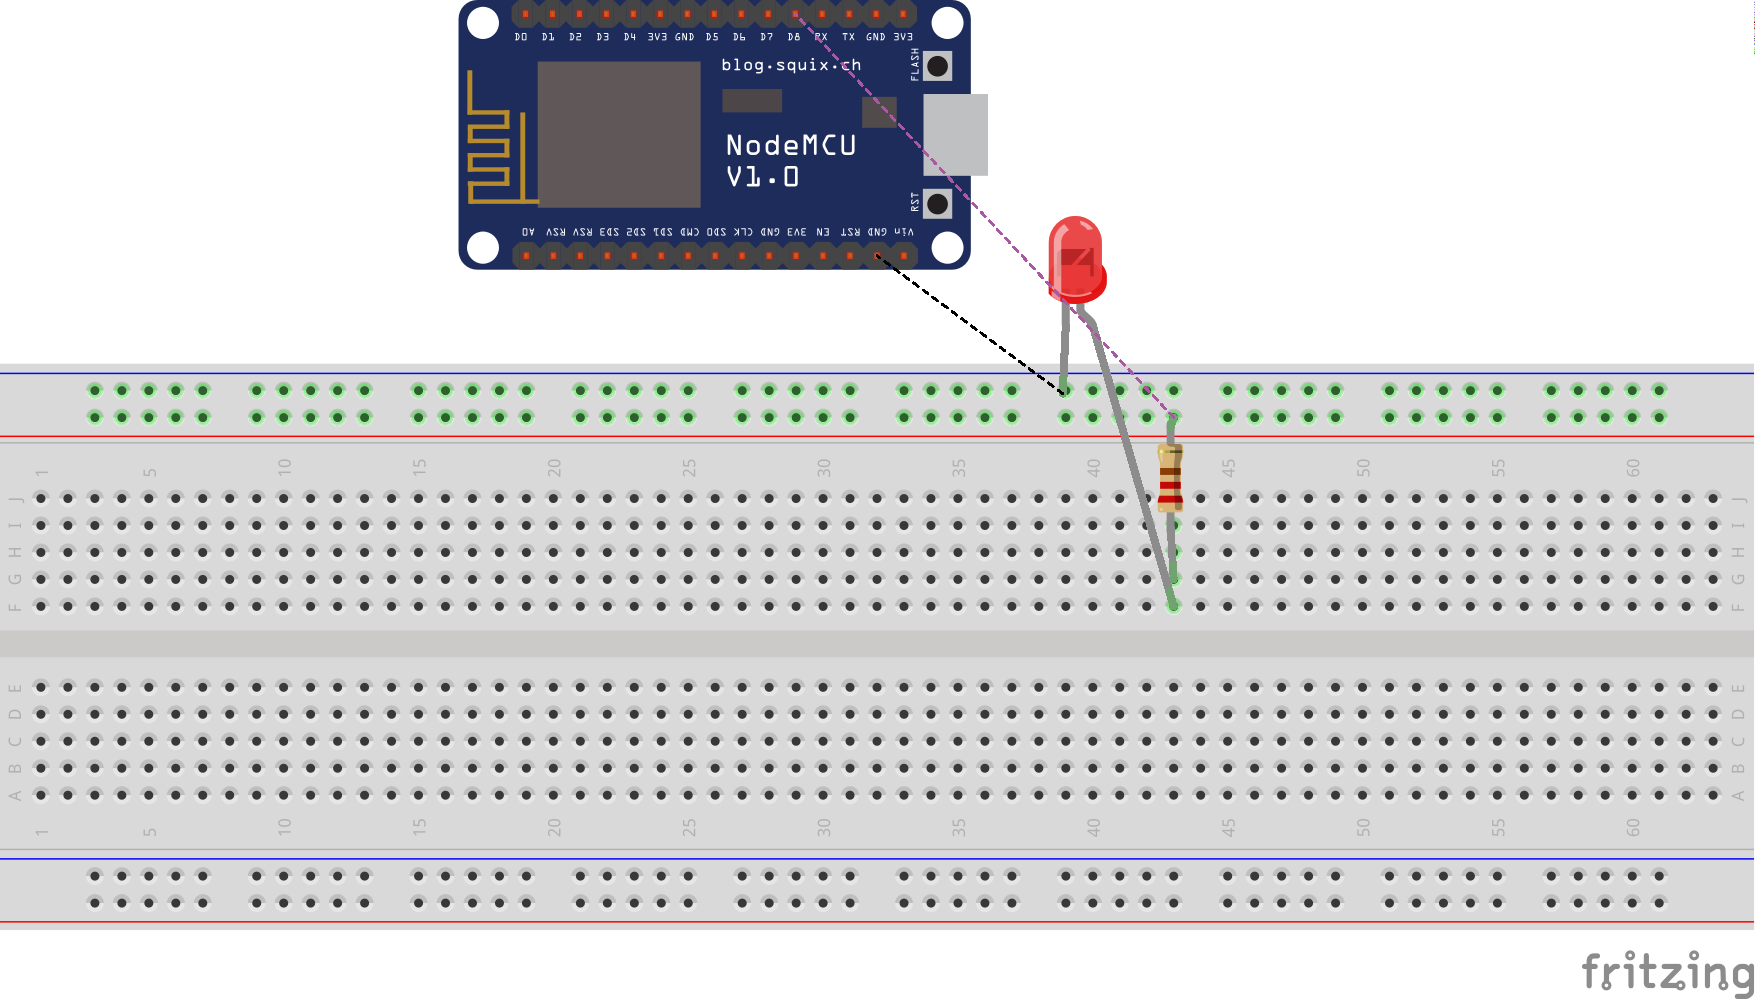
\includegraphics{../images/led-esp8266_bb.png}
\caption{breadboard}
\end{figure}

\begin{figure}
\centering
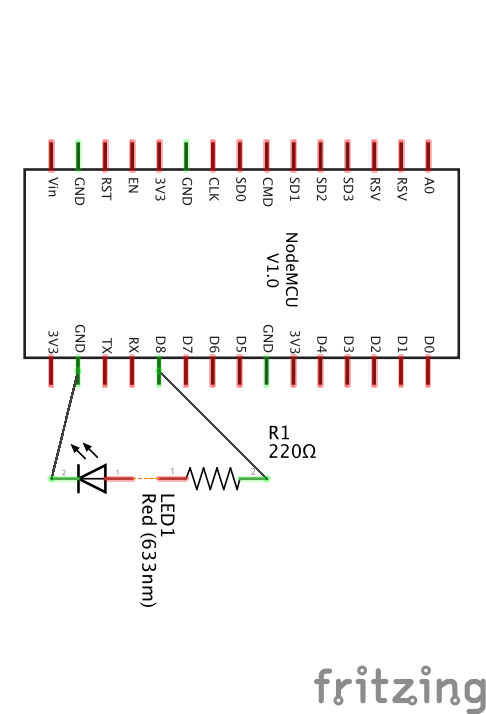
\includegraphics{../images/led-esp8266_schem.png}
\caption{schema}
\end{figure}

\paragraph{Real Time Clock}\label{real-time-clock}

Get the library urtc.py:

\begin{verbatim}
    wget https://raw.githubusercontent.com/adafruit/Adafruit-uRTC/master/urtc.py
    
\end{verbatim}

Place it on the esp8266

\begin{verbatim}
    cms robot put urtc.py
\end{verbatim}

Connect the board the following pins

\begin{verbatim}
SDA to pin 5 = D1
SCL to pin 4 = D2
\end{verbatim}

Login to the board

\begin{verbatim}
    cms robot login
    
\end{verbatim}

Execute the following code

\begin{verbatim}
    import machine
    i2c = machine.I2C(sda=machine.Pin(5), scl=machine.Pin(4))
    i2c.scan()
\end{verbatim}

\begin{quote}
\begin{verbatim}
  [87, 104]
\end{verbatim}
\end{quote}

\begin{verbatim}
    from urtc import DS3231
    t = DS3231(i2c)

    t.datetime()
\end{verbatim}

\begin{quote}
\begin{verbatim}
          DateTimeTuple(year=2000, month=1, day=1, 
                                           weekday=1, hour=0, minute=15,
                                           second=53, millisecond=None)
\end{verbatim}
\end{quote}

Assignment: Create an object orinted class and fill out the details
while using code from \texttt{urtc.py}

\begin{verbatim}
class Clock (object):
    def __init__(self, sda=5, scl=4)
    def get(self)
    def __str__(self)
    
c = Clock()
print (c.get())
print (c)
\end{verbatim}

\subsection{Resources}\label{resources}

\begin{verbatim}
    https://github.com/adafruit/Adafruit-uRTC/blob/master/urtc.py
    git clone https://github.com/adafruit/Adafruit-uRTC.git
\end{verbatim}

\subsection{Alternative boords}\label{alternative-boords}

\subsubsection{HUZZAH Feather esp8266}\label{huzzah-feather-esp8266}

Many different 8266 based alterantive boards exist. One of these boards
is the HUZZAH Feather. IT behaves the same as the other boards, but ay
be using differnt drivers and USB ports. The \emph{cms robot} command
line tool is clever enough to identify automatically if it is attached
and uses the appropriate settings. More documentation about this board
can be found at

\begin{itemize}
\tightlist
\item
  \href{https://learn.adafruit.com/adafruit-feather-huzzah-esp8266/using-nodemcu-lua}{doc}
\end{itemize}

This site has also many other examples and you can search for them with
keywords such as feather, esp8266, micropython.

An example on how to use the LED on the \emph{feather} is documented at

\begin{itemize}
\tightlist
\item
  \href{https://learn.adafruit.com/micropython-basics-blink-a-led/blink-led}{Feather
  HUZZAH ESP8266}
\end{itemize}

To place micropython on the feather you can plug in the to th eusb port.
The good thing about this board is that you do not need to press any
buttons as it detects the upload nicely. If not make sure to reset it or
for flasshing press both buttons. You can do the following:

Probe the board with:

\begin{verbatim}
cms robot probe
\end{verbatim}

Erasing the feather is simple as it has a bild in mechanism to detect if
it is going to be erased. Hence no reset button needs to be pressed:

\begin{verbatim}
cms robot flash erase
\end{verbatim}

Get the python image:

\begin{verbatim}
cms robot fetch python
\end{verbatim}

Flashing is conducted with 460800 baud, it will take about 15 seconds.
After flashing you should try to login:

\begin{verbatim}
cms robot login
\end{verbatim}

Set the boudrate to 115200:

\begin{verbatim}
CTRL-A CTRL-B>

*** baud: 
\end{verbatim}

type in:

\begin{verbatim}
115200 <ENTER>
\end{verbatim}

Make sure that echo is switched to OFF:

\begin{verbatim}
CTRL-A CTRL-C
\end{verbatim}

toogles it. Now you should see:

\begin{verbatim}
>>>
\end{verbatim}

Try typing in:

\begin{verbatim}
print("Hello")
\end{verbatim}

\subsection{Appendix}\label{appendix}

\subsection{Installing ESP8266 USB
drivers}\label{installing-esp8266-usb-drivers}

We provide here a section to explain which drivers we have tested on
various esp8266. Please note that if you have different versions you may
need different drivers. On OSX we found that we get good results with
the following commands

\begin{verbatim}
brew tap mengbo/ch340g-ch34g-ch34x-mac-os-x-driver https://github.com/mengbo/ch340g-ch34g-ch34x-mac-os-x-driver
brew cask install wch-ch34x-usb-serial-driver
\end{verbatim}

Start a new terminal after the driver has finished installing.

\begin{verbatim}
wget http://www.silabs.com/Support%20Documents/Software/Mac_OSX_VCP_Driver.zip
unzip Mac_OSX_VCP_Driver.zip
\end{verbatim}

Click on the driver install file contained inside the zip file and the
driver should start installing. Once the driver has finished installing,
make sure to start a new terminal.

Please remember that you need to close all terminals, as well as reboot
the computer to use the drivers. They will typically not work if you
have not rebooted.

For other boards that also use the CH340G chip the following page may
help:

\begin{itemize}
\tightlist
\item
  \url{http://kig.re/2014/12/31/how-to-use-arduino-nano-mini-pro-with-CH340G-on-mac-osx-yosemite.html}
\end{itemize}

\begin{fileremark}\url{https://github.com/cloudmesh/classes/blob/master/docs/source/lesson/iot/pi/pi.md}\end{fileremark}
\section{Raspberry PI 3}\label{raspberry-pi-3}

\subsection{Raspbery PI for IOT
(Gregor)}\label{raspbery-pi-for-iot-gregor}

\subsection{Hardware}\label{hardware}

see hardware page we have

\subsection{Installation}\label{installation}

\subsubsection{Erasing the SD Card}\label{erasing-the-sd-card}

Before you can install an OS on your sd card, you must erase it and put
it in the proper format.

\begin{enumerate}
\def\labelenumi{\arabic{enumi}.}
\tightlist
\item
  Insert your sd card into your micro-sd adapter and open Disk Utility
  with a spotlight search.
\item
  In the Disk Utility, right click the name of the sd card and select
  erase.
\item
  Name the sd card and format it as MS-DOS (FAT). Then click erase.
  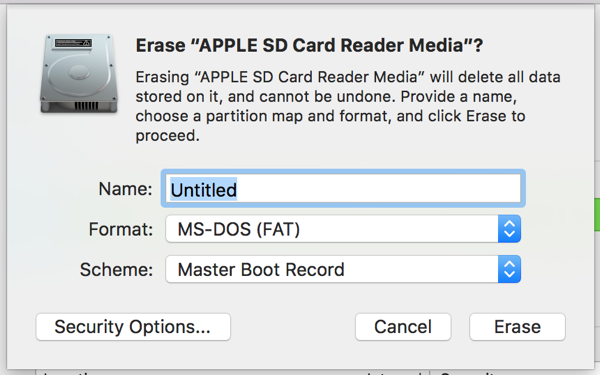
\includegraphics{../images/diskutil.png}
\item
  If it does not erase the first time, try again. It sometimes takes
  multiple tries to work.
\end{enumerate}

\subsubsection{Installation of NOOBS}\label{installation-of-noobs}

NOOBS is an OS that includes Raspian. The official descrition of
Raspbian can be found
\href{https://www.raspberrypi.org/downloads/raspbian/}{here}. It comes
pre-packaged with many useful programming tools, and is easy to use.

\begin{enumerate}
\def\labelenumi{\arabic{enumi}.}
\tightlist
\item
  Download Noobs
  \href{https://www.raspberrypi.org/downloads/noobs/}{here}. This will
  take around 30 minutes.
\item
  Go to your Finder and in Downloads, search for NOOBS.
\item
  Open the NOOBS folder and drag its contents into the sd card in the
  devices section. There should be 20 files and folders in the NOOBS
  folder. The download should take about 3 minutes.
\item
  Once installed, eject the sd card and put it in your raspberry pi.
\item
  Power up your raspberry and you will see a menu like this
\end{enumerate}

\begin{figure}
\centering
\includegraphics{../images/noobs.jpg}
\caption{}
\end{figure}

\begin{enumerate}
\def\labelenumi{\arabic{enumi}.}
\setcounter{enumi}{5}
\tightlist
\item
  Select Raspbian and click \texttt{Install\ (i)}
\end{enumerate}

\subsubsection{Installation of Dexter}\label{installation-of-dexter}

The version of Dexter that you want to flash onto your sd card is called
Raspbian for Robots. This is a Raspbian based os that is compatible with
the GrovePi board. It also comes with pre-installed Dexter Industries
software.

\begin{enumerate}
\def\labelenumi{\arabic{enumi}.}
\tightlist
\item
  First, download the most recent Dexter\_Industries\_jessie.zip file
  from
  \href{https://sourceforge.net/projects/dexterindustriesraspbianflavor/}{here}.
\item
  Once the file has downloaded, uncompress it and insert your sd card
  into the micro-sd adapter.
\item
  Open etcher and flash the uncompressed jessie image onto the sd card.
\end{enumerate}

\begin{figure}
\centering
\includegraphics{../images/etcher.png}
\caption{}
\end{figure}

\begin{enumerate}
\def\labelenumi{\arabic{enumi}.}
\setcounter{enumi}{3}
\tightlist
\item
  Eject your sd card and insert it into your raspberry pi.
\end{enumerate}

\subsection{Configure}\label{configure}

\subsubsection{Prepare OS}\label{prepare-os}

\subsection{Update}\label{update}

The following are essential updates:

\begin{verbatim}
sudo apt-get update
sudo apt-get upgrade
sudo apt-get install emacs
dpkg -l > ~/Desktop/packages.list
pip freeze > ~/Desktop/pip-freeze-initial.list
\end{verbatim}

The following are necessary for the scientific libraries, but they
require lots of space. Our sd cards do not have enough space for them.

\begin{verbatim}
sudo apt-get install build-essential python-dev python-distlib python-setuptools python-pip python-wheel libzmq-dev libgdal-dev
sudo apt-get install xsel xclip libxml2-dev libxslt-dev python-lxml python-h5py python-numexpr python-dateutil python-six python-tz python-bs4 python-html5lib python-openpyxl python-tables python-xlrd python-xlwt cython python-sqlalchemy python-xlsxwriter python-jinja2 python-boto python-gflags python-googleapi python-httplib2 python-zmq libspatialindex-dev
sudo pip install bottleneck rtree
\end{verbatim}

add to .bashrc

\begin{verbatim}
cd
git clone git://github.com/yyuu/pyenv.git .pyenv
echo 'export PYENV_ROOT="$HOME/.pyenv"' >> ~/.bashrc
echo 'export PATH="$PYENV_ROOT/bin:$PATH"' >> ~/.bashrc
echo 'eval "$(pyenv init -)"' >> ~/.bashrc
source ~/.bashrc

export PATH="/home/pi/.pyenv/bin:$PATH"
eval "$(pyenv init -)"
eval "$(pyenv virtualenv-init -)"

curl -L https://raw.githubusercontent.com/pyenv/pyenv-installer/master/bin/pyenv-installer | bash
\end{verbatim}

source

\subsubsection{Update to Python 3.6.1}\label{update-to-python-3.6.1}

\subsection{change python version}\label{change-python-version}

\begin{itemize}
\tightlist
\item
  {[}https://linuxconfig.org/how-to-change-from-default-to-alternative-python-version-on-debian-linux{]}
  (https://linuxconfig.org/how-to-change-from-default-to-alternative-python-version-on-debian-linux)
\end{itemize}

Upgrade setuptools for pip install with

\begin{verbatim}
    $ pip3 install --upgrade setuptools
    
\end{verbatim}

Test your python version with

\begin{verbatim}
    $ python --version
    
\end{verbatim}

Check your python version alternatives

\begin{verbatim}
    $ update-alternatives --list python
    
\end{verbatim}

If python2.7 is not in your alternatives, add it with

\begin{verbatim}
    $ sudo update-alternatives --install /usr/bin/python python /usr/bin/python2.7 1
    
\end{verbatim}

If python3.4 is not in your alternatives, add it with

\begin{verbatim}
    $ sudo update-alternatives --install /usr/bin/python python /usr/bin/python3.4 2
    
\end{verbatim}

Now make python3.4 to your default with

\begin{verbatim}
    update-alternatives --config python
\end{verbatim}

Select python3.4

\subsection{install 3.6.1}\label{install-3.6.1}

To install python 3.6.1, follow steps 1 and 2. This is unnecessary for
our purposes.

\begin{itemize}
\tightlist
\item
  \href{https://gist.github.com/dschep/24aa61672a2092246eaca2824400d37f}{better
  get 3.6.1}
\end{itemize}

\subsection{install cloudmesh.pi}\label{install-cloudmesh.pi}

pip install cloudmesh.pi

pip install cloudmesh.pi with

\begin{verbatim}
    $ git clone https://github.com/cloudmesh/cloudmesh.pi.git
    $ cd cloudmesh.pi
    $ sudo pip3 install .
\end{verbatim}

see how we do this in osx/linux can this be done on raspbery? if not
document update from source with altinstall

\subsubsection{Install scientific
Libraries}\label{install-scientific-libraries}

check if they are already installed we don't have enough space to
install all of these.

\begin{verbatim}
sudo apt-get install python-numpy python-matplotlib python-scipy python-sklearn python-pandas
\end{verbatim}

numpy\\
matplotlib\\
scipy\\
scikitlearn

\subsubsection{cloudmesh.pi (Jon)}\label{cloudmesh.pi-jon}

cloudmesh.pi is a repository for our GrovePi module classes. These
classes require Dexter software, so you need to either have Raspian for
Robots or download the software separately.

If you have Raspian for Robots, run the following in your terminal:

\begin{verbatim}
cd
mkdir github
cd github
git clone https://github.com/cloudmesh/cloudmesh.pi.git
cd cloudmesh.pi
sudo pip install .
\end{verbatim}

\subsubsection{Install VNC}\label{install-vnc}

describe how to install and configure VNC

\subsection{Sensors (Jon)}\label{sensors-jon}

\subsubsection{Grove Sensors (Jon)}\label{grove-sensors-jon}

we already have draft

\subsubsection{Non Grove Sensors (Jon)}\label{non-grove-sensors-jon}

Elegoo as example

\subsection{Notes To integrates}\label{notes-to-integrates}

\subsubsection{Connecting}\label{connecting}

Hostnames:

\begin{itemize}
\tightlist
\item
  raspberrypi.local
\item
  raspberrypi.
\end{itemize}

change

recovery.cmdline

forgot what these were:

\begin{verbatim}
runinstaller quiet ramdisk_size=32768 root=/dev/ram0 init=/init vt.cur_default=1 elevator=deadline
silentinstall runinstaller quiet ramdisk_size=32768 root=/dev/ram0 init=/init vt.cur_default=1 elevator=deadline
\end{verbatim}

Connect the cable

You will see the activity LEDs flash while the OS installs. Depending on
your SD-Card this can take up to 40-60 minutes.

\subsection{VLC on OSX}\label{vlc-on-osx}

\begin{itemize}
\item
  \url{http://www.videolan.org/vlc/index.en_GB.html}
\item
  \url{http://get.videolan.org/vlc/2.2.6/macosx/vlc-2.2.6.dmg}
\item
  \url{http://www.mybigideas.co.uk/RPi/RPiCamera/}
\item ~
  \subsection{Camera on Pi}\label{camera-on-pi}

  sudo apt-get install vlc
\item
  \url{https://www.raspberrypi.org/learning/getting-started-with-picamera/worksheet/}
\item
  \url{https://www.hackster.io/bestd25/pi-car-016e66}
\end{itemize}

\subsection{Streaming video}\label{streaming-video}

\begin{itemize}
\tightlist
\item
  \url{https://blog.miguelgrinberg.com/post/stream-video-from-the-raspberry-pi-camera-to-web-browsers-even-on-ios-and-android}
\end{itemize}

\subsection{Linux Commandline}\label{linux-commandline}

\begin{itemize}
\tightlist
\item
  \url{http://www.computerworld.com/article/2598082/linux/linux-linux-command-line-cheat-sheet.html}
\end{itemize}

\subsection{Enable SPI}\label{enable-spi}

go to the configuration interfaces and enable

\subsection{RTIMUlib2}\label{rtimulib2}

git clone https://github.com/RTIMULib/RTIMULib2.git cd RTIMULib

Add the following two lines to /etc/modules

\begin{verbatim}
i2c-bcm2708
i2c-dev
\end{verbatim}

reboot

\begin{verbatim}
ls /dev/i2c-*
sudo apt-get install i2c-tools

sudo i2cdetect -y 1
         0  1  2  3  4  5  6  7  8  9  a  b  c  d  e  f
00:          -- -- -- -- -- -- -- -- -- -- -- -- -- 
10: -- -- -- -- -- -- -- -- -- -- -- -- -- -- -- -- 
20: -- -- -- -- -- -- -- -- -- -- -- -- -- -- -- -- 
30: -- -- -- -- -- -- -- -- -- -- -- -- -- -- -- -- 
40: -- -- -- -- -- -- -- -- -- -- -- -- -- -- -- -- 
50: -- -- -- -- -- -- -- -- -- -- -- -- -- -- -- -- 
60: -- -- -- -- -- -- -- -- 68 -- -- -- -- -- -- -- 
70: -- -- -- -- -- -- -- --
\end{verbatim}

\begin{figure}
\centering
\includegraphics{images/rasp3.png}
\caption{Pinout}
\end{figure}

create a file /etc/udev/rules.d/90-i2c.rules and add the line:

\begin{verbatim}
KERNEL=="i2c-[0-7]",MODE="0666"
\end{verbatim}

note: does not work

instead we do

\begin{verbatim}
sudo chmod 666 /dev/i2c-1 
\end{verbatim}

Set the I2C bus speed to 400KHz by adding to /boot/config.txt:

\begin{verbatim}
dtparam=i2c1_baudrate=400000
\end{verbatim}

reboot. In terminal change directories to

\begin{verbatim}
cd /home/pi/github/RTIMULib2/RTIMULib/IMUDrivers
\end{verbatim}

and open

\begin{verbatim}
emacs RTIMUDefs.h
\end{verbatim}

In RTIMUDefs.h change

\begin{verbatim}
#define MPU9250_ID 0x71
\end{verbatim}

To

\begin{verbatim}
#define MPU9250_ID 0x73



cd /home/pi/github/RTIMULib2/RTIMULib
\end{verbatim}

In terminal

\begin{verbatim}
mkdir build
cd build
cmake ..
make -j4
sudo make install
sudo ldconfig
\end{verbatim}

\subsection{Compile RTIMULib Apps}\label{compile-rtimulib-apps}

\begin{verbatim}
cd /home/pi/github/RTIMULib2/Linux/RTIMULibCal
make clean; make -j4
sudo make install
cd /home/pi/github/RTIMULib2/Linux/RTIMULibDrive
make clean; make -j4
sudo make install
cd /home/pi/github/RTIMULib2/Linux/RTIMULibDrive10
make clean; make -j4
sudo make install
cd /home/pi/github/RTIMULib2/Linux/RTIMULibDrive11
make clean; make -j4
sudo make install


cd /home/pi/github/RTIMULib2/Linux/RTIMULibDemo    
qmake clean
make clean
qmake
make -j4
sudo make install
cd /home/pi/github/RTIMULib2/Linux/RTIMULibDemoGL
qmake clean
make clean
qmake
make -j4
sudo make install
\end{verbatim}

\subsection{Camera}\label{camera}

\begin{itemize}
\tightlist
\item
  \href{https://www.raspberrypi.org/learning/getting-started-with-picamera/worksheet/}{Camera
  Tutorial}
\end{itemize}

.

\begin{verbatim}
sudo apt-get install libjpeg-dev libtiff5-dev libjasper-dev libpng12-dev
sudo apt-get install libavcodec-dev libavformat-dev libswscale-dev libv4l-dev

sudo apt-get install libxvidcore-dev libx264-dev

sudo pip install virtualenv virtualenvwrapper
sudo rm -rf ~/.cache/pip
\end{verbatim}

copy into \textasciitilde{}/.profile:

\begin{verbatim}
 echo -e "\n# virtualenv and virtualenvwrapper" >> ~/.profile
 echo "export WORKON_HOME=$HOME/.virtualenvs" >> ~/.profile
 echo "source /usr/local/bin/virtualenvwrapper.sh" >> ~/.profile
\end{verbatim}

source \textasciitilde{}/.profile

\begin{verbatim}
mkvirtualenv cv -p python3
\end{verbatim}

workon cv

comandline has (cv) in front

\begin{verbatim}
pip install numpy

wget -O opencv.zip https://github.com/Itseez/opencv/archive/3.1.0.zip
wget -O opencv_contrib.zip https://github.com/Itseez/opencv_contrib/archive/3.1.0.zip
unzip opencv.zip
unzip opencv_contrib.zip
\end{verbatim}

\subsection{Lessons and Projects}\label{lessons-and-projects}

\begin{itemize}
\tightlist
\item
  \href{https://www.raspberrypi.org/learning/getting-started-with-guis/worksheet/}{Gui}\\
\item
  \href{https://www.raspberrypi.org/learning/getting-started-with-guis/}{Solder}\\
\item
  \href{https://www.raspberrypi.org/blog/an-image-processing-robot-for-robocup-junior/}{PI
  Camera Line Follower}\\
\item
  \href{https://circuitdigest.com/microcontroller-projects/web-controlled-raspberry-pi-surveillance-robot}{Pi
  car flask}
\end{itemize}

\subsection{OTHER TO BE INTEGRATED}\label{other-to-be-integrated}

\subsubsection{PI emulator on Windows}\label{pi-emulator-on-windows}

We have not yet tried it, but we like to hear back from you on
experiences with

\begin{itemize}
\tightlist
\item
  https://sourceforge.net/projects/rpiqemuwindows/
\end{itemize}

\subsubsection{Scratch}\label{scratch}

\begin{itemize}
\tightlist
\item
  \href{https://github.com/DexterInd/GrovePi/tree/master/Software/Scratch}{scratch}
\end{itemize}

\subsection{Web Server}\label{web-server}

\begin{itemize}
\tightlist
\item
  \href{https://www.raspberrypi.org/learning/python-web-server-with-flask/worksheet/}{Web
  Server Flask}
\end{itemize}

\begin{fileremark}\url{https://github.com/cloudmesh/classes/blob/master/docs/source/lesson/iot/pi/dexter.md}\end{fileremark}
\section{Dexter}\label{dexter}

\subsection{Creating an SD Card}\label{creating-an-sd-card}

\subsubsection{OSX}\label{osx}

First, install Etcher from \href{https://etcher.io/}{etcher.io} which
allows you to flash images onto the SD card. When flashing make sure you
only attach one USB SD card reader/wroiter or use the build in SD card
slot provided in some Mac's.

The version of etcher we used is

\begin{itemize}
\tightlist
\item
  \href{https://github.com/resin-io/etcher/releases/download/v1.1.1/Etcher-1.1.1-darwin-x64.dmg}{Etcher-1.1.1-darwin-x64.dmg}
\end{itemize}

Make sure to check if there is a newer version

\subsubsection{Dexter Rasbian}\label{dexter-rasbian}

Dexter provides a special image that contains the drivers and sample
programs for the GrovePi shield. We had some issues installing it on a
plain Raspbian OS, thus we recommend that you use dexters version if you
use the GrovePi shield. It is available from

\begin{itemize}
\tightlist
\item
  \href{http://sourceforge.net/projects/dexterindustriesraspbianflavor/}{Google
  Drive}
\item
  \href{http://sourceforge.net/projects/dexterindustriesraspbianflavor/}{Sourceforge}
\end{itemize}

Detailed information on how to generate an SD card while using your OS
is provided at

\begin{itemize}
\tightlist
\item
  \url{https://www.dexterindustries.com/howto/install-raspbian-for-robots-image-on-an-sd-card/}
\end{itemize}

\subsubsection{Github}\label{github}

Dexter maintains a github repository that includes their code for the
shield and many other projects at

\begin{itemize}
\tightlist
\item
  \url{https://github.com/DexterInd}
\end{itemize}

\subsubsection{Cloning Grove PI}\label{cloning-grove-pi}

To clone the GrovePI library on other computers you can use the command

\begin{verbatim}
git clone https://github.com/DexterInd/GrovePi.git
\end{verbatim}

\subsubsection{Dexter Sample programs}\label{dexter-sample-programs}

Dexter maintains all GrovePi related programs at

\begin{itemize}
\tightlist
\item
  \url{https://github.com/DexterInd/GrovePi}
\end{itemize}

The python related programs are in a subdirectory at

\begin{itemize}
\tightlist
\item
  \url{https://github.com/DexterInd/GrovePi/tree/master/Software/Python}
\end{itemize}

Here you find many programs and for a complete list visit that link.
Dependent on the sensors and actuators you have, inspect some programs.
Some of them may inspire you to purchase some sensors.

We have developed a partial library of GrovePi module classes at

\begin{itemize}
\tightlist
\item
  \url{https://github.com/cloudmesh/cloudmesh.pi/tree/master/cloudmesh/pi}
\end{itemize}

\begin{fileremark}\url{https://github.com/cloudmesh/classes/blob/master/docs/source/lesson/iot/pi/grovepi.md}\end{fileremark}
\section{GrovePi Modules}\label{grovepi-modules}

\subsection{Intro}\label{intro}

\begin{itemize}
\tightlist
\item
  \href{http://www.instructables.com/id/Basic-Electronics}{Electronics}:
  An introduction to the basic principals of electronics.
\item
  \href{https://learn.sparkfun.com/tutorials/voltage-current-resistance-and-ohms-law}{Volatage}:
  An introduction to the physics of electricity.
\item
  \href{https://info-ee.eps.surrey.ac.uk/Teaching/Unix/index.html}{Unix}:
  An introduction to the Unix os.
\item
  \href{https://github.com/DexterInd/GrovePi/tree/master/Software/Python}{grove
  examples}: A list of Dexter Industries example code for GrovePi
  modules.
\item
  \href{https://github.com/cloudmesh/cloudmesh.pi/tree/master/cloudmesh/pi}{GrovePi
  module classes}: A repository for the GrovePi module classes.
\end{itemize}

\subsection{LED}\label{led}

An LED is the simplest possible module for a raspberry pi, as it is
responsive only to the provided power. For an LED to emit light, it must
be exposed to a voltage greater than a certain threshold value. Above
this voltage, the conductivity of the diode increases exponentially and
its brightness increases likewise. If the current through the LED
becomes too high, the LED will burn out. The following link leads to a
tutorial from Dexter Industries for the LED module.

\begin{itemize}
\tightlist
\item
  \href{https://www.dexterindustries.com/GrovePi/projects-for-the-raspberry-pi/raspberry-pi-led-tutorial/}{Dexter
  LED tutorial}
\end{itemize}

Connect the LED To a digital port. The following code describes an LED
class. Since it is connected to a digital output, the voltage has only
two states, on and off. The default port for the LED class is D3. The
code for the \texttt{LED} class can be found here:

\begin{itemize}
\tightlist
\item
  \href{https://github.com/cloudmesh/cloudmesh.pi/blob/master/cloudmesh/pi/led.py}{LED
  Class}
\end{itemize}

\begin{figure}
\centering
\includegraphics{../images/grovepi/led.jpg}
\caption{LED}
\end{figure}

\subsection{Buzzer}\label{buzzer}

Connect the buzzer to a digital port. The default port for the Buzzer
class is D3. You will notice that the Buzzer class and the LED class are
interchangeable. This is because they work on the same digital
principal. Their two values are on and off. The code for the
\texttt{Buzzer} class can be found here:

\begin{itemize}
\tightlist
\item
  \href{https://github.com/cloudmesh/cloudmesh.pi/blob/master/cloudmesh/pi/buzzer.py}{Buzzer
  Class}
\end{itemize}

\begin{figure}
\centering
\includegraphics{../images/grovepi/buzzer.jpg}
\caption{Buzzer}
\end{figure}

\subsection{Relay}\label{relay}

The relay acts as a switch in a circuit. When the value on the relay is
1, it allows current to flow through it. When the value is 0, the relay
breaks the circuit and the current stops. Connect the relay to a digital
port. The default digital port is D4. The \texttt{Relay} class can be
found here:

\begin{itemize}
\tightlist
\item
  \href{https://github.com/cloudmesh/cloudmesh.pi/blob/master/cloudmesh/pi/relay.py}{Relay
  Class}
\end{itemize}

\begin{figure}
\centering
\includegraphics{../images/grovepi/relay.jpg}
\caption{Relay}
\end{figure}

\subsection{Light Sensor}\label{light-sensor}

The light sensor measures ligh intensity and returns a value between 0
and 1023. Connect the light sensor to an analog port. The default port
is A0. The analog port allows the light sensor to return a range of
values. The \texttt{LightSensor} class can be found here:

\begin{itemize}
\tightlist
\item
  \href{https://github.com/cloudmesh/cloudmesh.pi/blob/master/cloudmesh/pi/light.py}{LightSensor
  Class}
\end{itemize}

\begin{figure}
\centering
\includegraphics{../images/grovepi/light.jpg}
\caption{Light Sensor}
\end{figure}

\subsection{Rotary Angle Sensor}\label{rotary-angle-sensor}

The rotary angle sensor measures the angle to which it is turned.
Connect the sensor to an analog port. Port A0 is the default. The
\texttt{RotarySensor} class can be found here:

\begin{itemize}
\tightlist
\item
  \href{https://github.com/cloudmesh/cloudmesh.pi/blob/master/cloudmesh/pi/rotary.py}{RotarySensor
  Class}
\end{itemize}

\begin{figure}
\centering
\includegraphics{../images/grovepi/rotary.jpg}
\caption{Rotary Angle Sensor}
\end{figure}

\subsection{Barometer}\label{barometer}

Connect the barometer to an I2C port. In addition to pressure, the
GrovePi barometer measures temperature in Fahrenheit and Celcius. The
\texttt{Barometer} class can be found here.

\begin{itemize}
\tightlist
\item
  \href{https://github.com/cloudmesh/cloudmesh.pi/blob/master/cloudmesh/pi/barometer.py}{Barometer
  Class}
\end{itemize}

\begin{figure}
\centering
\includegraphics{../images/grovepi/barometer.jpg}
\caption{Barometer}
\end{figure}

\subsection{Distance Sensor}\label{distance-sensor}

Connect the distance sensor to a digital port. The grovepi module has a
built-in function to read the distance from the distance sensor, but it
is improperly calibrated, so this DistanceSensor class has a calibration
based on experimental data. The \texttt{DistanceSensor} class can be
found here:

\begin{itemize}
\tightlist
\item
  \href{https://github.com/cloudmesh/cloudmesh.pi/blob/master/cloudmesh/pi/distance.py}{DistanceSensor
  Class}
\end{itemize}

\begin{figure}
\centering
\includegraphics{../images/grovepi/distance.jpg}
\caption{Distance Sensor}
\end{figure}

\subsection{Temperature Sensor}\label{temperature-sensor}

The temperature sensor measures both temperature and humidity. Connect
the temperature sensor to a digital port. D7 is the default port. The
\texttt{TemperatureSensor} class can be found here:

\begin{itemize}
\tightlist
\item
  \href{https://github.com/cloudmesh/cloudmesh.pi/blob/master/cloudmesh/pi/temperature.py}{TemperatureSensor
  Class}
\end{itemize}

\begin{figure}
\centering
\includegraphics{../images/grovepi/temperature.jpg}
\caption{Temperature Sensor}
\end{figure}

\subsection{Heartbeat Sensor}\label{heartbeat-sensor}

Connect the heartbeat sensor to an I2C port. The heartbeat sensor
returns the heart rate of the wearer. The \texttt{HeartbeatSensor} class
can be found here:

\begin{itemize}
\tightlist
\item
  \href{https://github.com/cloudmesh/cloudmesh.pi/blob/master/cloudmesh/pi/heartbeat.py}{HearbeatSensor
  Class}
\end{itemize}

\begin{figure}
\centering
\includegraphics{../images/grovepi/heartbeat.jpg}
\caption{image}
\end{figure}

\subsection{Joystick}\label{joystick}

Connect the joystick to an analog port. A0 is the default port. The
joystick has an x, y, and click status based on the current state of the
module. The \texttt{Joystick} class can be found here:

\begin{itemize}
\tightlist
\item
  \href{https://github.com/cloudmesh/cloudmesh.pi/blob/master/cloudmesh/pi/joystick.py}{Joystick
  Class}
\end{itemize}

\begin{figure}
\centering
\includegraphics{../images/grovepi/joystick.jpg}
\caption{image}
\end{figure}

\subsection{LCD Screen}\label{lcd-screen}

The LCD screen can be used to display text and colors. In order to use
it, plug it into one of the I2C ports. The \texttt{LCD} class can be
found here:

\begin{itemize}
\tightlist
\item
  \href{https://github.com/cloudmesh/cloudmesh.pi/blob/master/cloudmesh/pi/lcd.py}{LCD
  Class}
\end{itemize}

\begin{figure}
\centering
\includegraphics{../images/grovepi/lcd.jpg}
\caption{LCD Screen}
\end{figure}

\subsection{Moisture Sensor}\label{moisture-sensor}

Connect the moisture sensor to an analog port. The default port is A0.
The \texttt{MoistureSensor} class can be found here:

\begin{itemize}
\tightlist
\item
  \href{https://github.com/cloudmesh/cloudmesh.pi/blob/master/cloudmesh/pi/moisture.py}{MoistureSensor
  Class}
\end{itemize}

\begin{figure}
\centering
\includegraphics{../images/grovepi/moisture.jpg}
\caption{Moisture Sensor}
\end{figure}

An example of the implimentation of the moisture sensor from Dexter
Industries can be found
\href{https://github.com/DexterInd/GrovePi/blob/master/Projects/plant_monitor/plant_project.py}{here}.
The program is meant to measure the environmental conditions that affect
plant growth.

\subsection{Water Sensor}\label{water-sensor}

The water sensor measures the amount of water in the environment of the
sensor. Connect the sensor to a digital point. D2 is the default port.
The \texttt{WaterSensor} class can be found here:

\begin{itemize}
\tightlist
\item
  \href{https://github.com/cloudmesh/cloudmesh.pi/blob/master/cloudmesh/pi/water.py}{WaterSensor
  Class}
\end{itemize}

\begin{figure}
\centering
\includegraphics{../images/grovepi/water.jpg}
\caption{Water Sensor}
\end{figure}

\begin{fileremark}\url{https://github.com/cloudmesh/classes/blob/master/docs/source/lesson/iot/pi/sensors.md}\end{fileremark}
\section{Sensors}\label{sensors}

This section is to be completed by the students of the class.

Task is to develop an object oriented class for one of the sensors. An
example for such a class can be found at:

\begin{itemize}
\tightlist
\item
  \url{https://github.com/cloudmesh/cloudmesh.pi/blob/master/cloudmesh/pi/led.py}
\end{itemize}

\subsection{Compass}\label{compass}

TODO: which compas sensor

The default pins are defined in variants/nodemcu/pins\_arduino.h as GPIO

\begin{verbatim}
SDA=4 
SCL=5
D1=5 
D2=4.
\end{verbatim}

You can also choose the pins yourself using the I2C constructor
Wire.begin(int sda, int scl);

\FILENAME

\section{VNC}\label{vnc}

\textbf{Note:} \emph{If you like to connect to your Raspberry from your
laptop, we recommend to use VNC. If you rather like to connect a monitor
and keyboard as well as a mouse to the Raspberry, you can skip the steps
with the VNC update.}

\subsection{Setting up VNC}\label{setting-up-vnc}

We had some issues with the installed version of VNC that is customized
for connecting a Laptop via the ethernet cable to the PI. However as we
connect wirelessly, our setup is slightly diffrent. The easiset way that
we found is to update the Raspbian OS as follows. In a terminal type

\begin{verbatim}
sudo apt-get update
sudo apt-get install realvnc-vnc-server 
sudo apt-get install realvnc-vnc-viewer
\end{verbatim}

Next you enable the VNC server in the configuration panel via the
Rasbian GUI by selecting

\begin{verbatim}
 Menu > 
    Preferences > 
       Raspberry Pi Configuration > 
          Interfaces.
\end{verbatim}

Here you toggle the VNC service to enabled. As we are already at it in
our setup we enabled all other services, especially those that deal with
Grove sensor related bins and wires.

Next reboot and double check if the settings are preseved after the
reboot

\subsubsection{Install VNC on OSX}\label{install-vnc-on-osx}

To install a vnc server of your liking on your Mac. You find one at

\begin{itemize}
\tightlist
\item
  \href{http://www.realvnc.com/download/vnc/latest/\%5D}{http://www.realvnc.com/download/vnc/latest/}
\end{itemize}

Be sure to download the version of the VNC Viewer for the computer you
are going to use to virtually control the Pi (there is a version listed
for Raspberry Pi-- don't download this one. For us this is the Mac
version.)

\subsubsection{Run VNC Viewer on OSX}\label{run-vnc-viewer-on-osx}

Once you have downloaded the VNC viewer installed it you can open the
program. Next you can start vnc viewer and enter the ip address of your
raspberry. Make sure you are on the same network. You can find the
address by using ifconfig.

\begin{fileremark}\url{https://github.com/cloudmesh/classes/blob/master/docs/source/lesson/iot/turtle.md}\end{fileremark}
\section{Turtle Graphics}\label{turtle-graphics}

\subsection{Demo}\label{demo}

Python comes with a nice demonstartion program that allows you to learn
some simple programming concepts while moving a turtle on the screen. It
can be started with

\begin{verbatim}
python -m turtledemo
\end{verbatim}

\subsection{Program example}\label{program-example}

You can also create programs with your favorite editor and run it. Let
us put the following code into the program \texttt{turtle\_demo.py}.
Never save a file with the name \texttt{turtle.py} because python will
import it instead of the built-in turtle import that you need.

\begin{verbatim}
import turtle

window = turtle.Screen() 
robot = turtle.Turtle() 

robot.forward(50)   # Moves forward 50 pixels
robot.right(90)     # Rotate clockwise by 90 degrees

robot.forward(50)
robot.right(90)

robot.forward(50)
robot.right(90)

robot.forward(50)
robot.right(90)

turtle.done()

window.mainloop()
\end{verbatim}

After saving it you can run it from a terminal with

\begin{verbatim}
$ python turtle_demo.py
\end{verbatim}

\subsection{Shape}\label{shape}

\begin{verbatim}
shapes: “arrow”, “turtle”, “circle”, “square”, “triangle”, “classic”
\end{verbatim}

You can change the shape of your turtle to any of these shapes with the
Turtle method \texttt{shape(name)}. For example, if you have an instance
of the Turtle class called \texttt{robot}, you can make it appear as a
turtle by calling \texttt{robot.shape("turtle")}.

You can add your own shapes with the following functions:

\begin{verbatim}
turtle.register_shape(name, shape=None)

turtle.addshape(name, shape=None)
\end{verbatim}

There are three different ways to call this function:

name is the name of a gif-file and shape is None: Install the
corresponding image shape.

\begin{verbatim}
window.register_shape("turtle.gif")
\end{verbatim}

Note: Image shapes do not rotate when turning the turtle, so they do not
display the heading of the turtle!

name is an arbitrary string and shape is a tuple of pairs of
coordinates: Install the corresponding polygon shape.

\begin{verbatim}
window.register_shape("triangle", ((5,-3), (0,5), (-5,-3)))
\end{verbatim}

name is an arbitrary string and shape is a (compound) Shape object:
Install the corresponding compound shape.

Add a turtle shape to TurtleScreen's shapelist. Only thusly registered
shapes can be used by issuing the command shape(shapename).

\subsection{Links}\label{links}

\begin{itemize}
\tightlist
\item
  http://openbookproject.net/thinkcs/python/english3e/hello\_little\_turtles.html
\item
  \url{https://docs.python.org/3/library/turtle.html}
\end{itemize}

\section{Robot Dance Simulator}\label{robot-dance-simulator}

\begin{verbatim}
cms robot dance dance.txt
\end{verbatim}

\section{Scratch}\label{scratch}

\begin{itemize}
\tightlist
\item
  \href{https://scratch.mit.edu/scratchr2/static/sa/Scratch-456.0.2.dmg}{Scratch}
\end{itemize}

\section{MBlock}\label{mblock}

\begin{itemize}
\tightlist
\item
  \href{http://www.mblock.cc/download/}{MBlock}
\end{itemize}

\FILENAME

\section{Tools}\label{tools}

\begin{itemize}
\item
  \textbf{Terminal}: On OSX, when you navigate to the search
  magnification glass, you can type in \emph{terminal} to start it. A
  terminal allows you to execute a number of commands to interact with
  the computer from a commandline interface, e.g.~the terminal.
\item
  \href{https://linuxconfig.org/bash-scripting-tutorial}{Bash} it the
  command language used in terminal.
\item
  \href{https://cloudmesh.github.io/classes/lesson/prg/pyenv.html?highlight=xcode\#install-pyenv-on-osxhttps://cloudmesh.github.io/classes/lesson/prg/pyenv.html?highlight=xcode\#install-pyenv-on-osx}{Pyenv}
  allows to manage multiple versions of python easily.
  \href{https://github.com/pyenv/pyenv\#how-it-works}{Pyenv link}
\item
  \href{https://cloudmesh.github.io/classes/lesson/prg/pyenv.html?highlight=xcode\#install-pyenv-on-osxhttps://cloudmesh.github.io/classes/lesson/prg/pyenv.html?highlight=xcode\#install-pyenv-on-osx}{XCode}
  is an integrated development environment for macOS containing a suite
  of software development tools developed by Apple for developing
  software for macOS, iOS, watchOS and tvOS.
\item
  \href{https://brew.sh}{Homebrew} is a \emph{package manager} for OS X
  which lets the user \emph{install software} from \emph{UNIX} and
  \emph{open source software} that is not included in OSX.
\item
  \href{https://www.jetbrains.com/pycharm/download/download-thanks.html?platform=mac\&code=PCC}{pyCharm}:
  is an Integrated Development Environment for Python.
\item
  \emph{Matplotlib}: Matplotlib is a libarry that allows us to create
  nice graphs in python. As we typically install python with virtualenv,
  we need to configure matplotlib properly to use it. The easiest way to
  do this is to execute the following commands. After you run them you
  can use matplotlib.

\begin{verbatim}
$ pip install numpy
$ pip install matplotlib
$ echo "backend : TkAgg" > ~/.matplotlib/matplotlibrc
\end{verbatim}
\item
  \href{https://macdown.uranusjr.com/}{Macdown} a macdown editor for OSX
\item
  \href{https://blog.ghost.org/markdown/}{Markdown} (from Markdown)
\item
  \href{http://oracc.museum.upenn.edu/doc/help/usingemacs/aquamacs/}{AquaEmacs}
  (from Aquaemacs)
\item
  \href{http://marvelmind.com/}{Marvelmind} (from Marvelmind if you have
  marvelmind positioning sensors which are optional)
\item
  \href{https://www.arduino.cc/en/guide/macOSX}{Arduino} (from Arduino
  if you like to use their interface to access the esp8266 boards)
\item
  \href{https://computers.tutsplus.com/tutorials/40-terminal-tips-and-tricks-you-never-thought-you-needed--mac-51192}{40
  OSX Terminal Tricks}
\end{itemize}

\subsection{Markdown}\label{markdown}

MarkDown is a format convention that produces nicely formated text with
simple ASCII text. Markdown has very good support for editors that
render the final output in a view window next to the editor pane. Two
such editors are

\begin{itemize}
\tightlist
\item
  \href{https://macdown.uranusjr.com/}{Macdown}: MacDown provides a nice
  integrated editor that works well.
\item
  \href{https://www.jetbrains.com/pycharm/download/download-thanks.html?platform=mac\&code=PCC}{pyCharm}:
  We have successfully used Vladimir Schhneiders
  \href{https://plugins.jetbrains.com/plugin/7896-markdown-navigator}{Markdown
  Navigator plugin}. Once installes you click on a .md file pycharm will
  automatically ask to install the plugins from Markdown for you.
\end{itemize}

A detailed set of syntax rules can be found at: \textbf{BUG: LINK TO
MARKDOWN SYNTAX MISSING}

The following are some basic examples

\begin{itemize}
\tightlist
\item
  To \emph{empazise} a text you use \texttt{*empasize*}
\item
  To make text \textbf{bold} use \texttt{**bold**}
\item
  To make text \textbf{\emph{bold-and-emphasize}} use
  \texttt{***bold-and-emphasize***}
\item
  To create a hyperlink use \texttt{{[}Google{]}(https://google.com)}
  which will result in \href{https://google.com}{Google}
\item
  To include an image use \texttt{!{[}Bracketed\ Text{]}(link)}
\end{itemize}

A list can be created by item starting with ``*``, a''-``, or a''+" or a
number

\begin{verbatim}
1. one
2. two
\end{verbatim}

\begin{enumerate}
\def\labelenumi{\arabic{enumi}.}
\item
  one
\item
  two

\begin{verbatim}
* one
* two
\end{verbatim}
\end{enumerate}

\begin{itemize}
\tightlist
\item
  one
\item
  two
\end{itemize}

If you need to indent items underneath already bulleted items, precede
the indent items with four spaces and they will be nested under the item
above them.

To qoute textc precede it with a ``\textgreater{}''.

\begin{verbatim}
> Quote
\end{verbatim}

\begin{quote}
Quote
\end{quote}

Other syntax options can be found in the Format drop-down at the top of
the screen between View and Plug-ins of macdown.

\subsection{Aquamacs}\label{aquamacs}

There are many different versions of emacs available on OSX. Aquamacs is
often used as it integrates nicely with the OSX GUI interface.

\begin{itemize}
\tightlist
\item
  \href{http://aquamacs.org/download.shtml}{AquaEmacs}
\end{itemize}

\emph{Aquamacs} is a program for Mac devices which allows the user to
edit text, HTML, LaTeX, C++, Java, Python, R, Perl, Ruby, PHP, and more.
Aquaemacs integrates well with OSX and provides many functions through a
menu. You will mostly be using the File, Edit, menus or toolbar icons.

Emacs provides convenient keyboard shortcuts, most of which are
combinations with the Control or Meta key (The Meta key is the ESC key).
If you accidentally end up doing something wrong simply press
\texttt{CTRL-g} to get out without issue. Other Keyboard Shortcuts
include:

\begin{itemize}
\item
  \texttt{CTRL-x\ u} or File\textgreater{}Undo will cancel any command
  that you did not want done. (CHECK)
\item
  \texttt{ESC-g} will cancel any command you are in the middle of.
\item
  You can break paragraph lines with \texttt{Ctrl-x\ w}, where
  \texttt{w} will wrap text around word boundaries.
\item
  To delete text to the end of the current word, press \texttt{ESC-d}.
\item
  to delete the whole line from the position of the cursor to the end,
  press \texttt{CTRL-k}.
\end{itemize}

\subsection{Bash}\label{bash}

Bash is preinstalled in OSX. A \emph{bash} script contains
\emph{commands} in plain text. In order to create a bash script please
decide for a convenient name. Ltes assume we name our script
\emph{myscript}. Than you can create and edit such a script with

\begin{verbatim}
$ touch myscript.sh
$ emacs myscripts.sh
\end{verbatim}

Next you need to add the following line to the top ogf the script:

\begin{verbatim}
!# /bin/bash
\end{verbatim}

To demonstrate how to continue writing a script we will be using the
bash \texttt{echo} command that allows you to print text. Lets make the
second line

\begin{verbatim}
echo "Hello World"
\end{verbatim}

You can now save and start executing your script. Click ``File'' and
then ``Save''. Open Terminal and type in \texttt{cd} followed by the
name of the folder you put the document in. Now we need to execute the
script.

\emph{Executing} a Bash script is rather easy. In order to execute a
script, we need to first execute the \emph{permission set}. In order to
give Terminal permission to read/execute a Bash script, you have to type

\begin{verbatim}
chmod u+x myscript.sh
\end{verbatim}

After the script has been granted permission to be executed, you can
test it by typing

\begin{verbatim}
./myscript.sh
\end{verbatim}

into the terminal. You will see it prints

\begin{verbatim}
Hello World
\end{verbatim}

\subsection{Arduino}\label{arduino}

This instalation is optional. In the event that there is a TTY error,
you will need to install Arduino, since your Mac may be missing some
drivers that are included in Arduino. Simply go to
\href{https://www.arduino.cc/en/guide/macOSX}{Arduino} and follow the
instalation instructions.

\subsection{OSX Terminal}\label{osx-terminal}

\href{https://learn.sparkfun.com/tutorials/terminal-basics/coolterm-windows-mac-linux}{CoolTerm}

download \url{http://freeware.the-meiers.org/CoolTermMac.zip}



%----------------------------------------------------------------------------------------
%	CLOUD
%----------------------------------------------------------------------------------------

\part{i5xx Cloud}

\chapterimage{chapter_head_2.png} % Chapter heading image

\chapter{Cloud}

\chapter{Fundamentals}

\begin{fileremark}\url{https://github.com/cloudmesh/classes/blob/master/docs/source/icloud/2017/course/fundamentals.rst}\end{fileremark}
\section{Cloud Computing
Fundamentals}\label{cloud-computing-fundamentals}

\begin{itemize}
\tightlist
\item
  6 Video lectures (48 minutes 20 seconds)
\end{itemize}

\subsection{Course Info}\label{course-info}

Prof. Judy Qiu covers basic information about Unit 1, including lecture
schedule and homework submissions. Key cloud computing topics are
highlighted. A selection of recommended and required textbooks is given,
followed by an overview of the course structure.

\begin{itemize}
\tightlist
\item
  Video: \href{https://www.youtube.com/watch?v=Kde5YVUwDTQ}{Youtube}
  (13:13)
\end{itemize}

\begin{itemize}
\tightlist
\item
  Slide:
  \href{https://drive.google.com/open?id=0B88HKpainTSfYjU4QzdDSms0Nk0}{PDF}
\end{itemize}

\subsection{Introduction}\label{introduction}

Changes in computing technology for the past five decades are discussed.
The rise of Big Data is shown in terms of its growth and significance. A
prediction is made that the paradigm which has held `til now of
individual researchers with personal computers will give way to
communities of researchers organizing through clouds. A more in-depth
look at Unit 1 follows, focusing on the chapters from Distributed and
Cloud Computing: From Parallel Processing to the Internet of Things.

\begin{itemize}
\tightlist
\item
  Video: \href{https://www.youtube.com/watch?v=5lKj8_nqj9k}{Youtube}
  (8:31)
\end{itemize}

\subsection{Data Center Model}\label{data-center-model}

A look at what truly defines a `cloud'. Advantages like scalability and
cost-effectiveness have promulgated commercial cloud offerings such as
Amazon EC2. Cloud architecture as divided into three layers:
Infrastructure as a Service, Platform as a Service, and Software as a
Service. AzureBlast is used as an example of how to utilize the cloud
setup. Certain misconceptions about clouds are then presented for
further discussion.

\begin{itemize}
\tightlist
\item
  Video: \href{https://www.youtube.com/watch?v=6Hq_LuLB-RU}{Youtube}
  (8:08)
\end{itemize}

\subsection{Data Intensive Sciences}\label{data-intensive-sciences}

Some time is spent analyzing the current age of vast data growth, where
business, science, and consumer activity has seen an explosion of stored
data measured in exobytes. In response to this, the way we conduct
scientific research has also undergone an upgrade. However, the average
scientist would rather focus on their own research rather than spend
time trying to learn different methods of cloud and supercomputing.

\begin{itemize}
\tightlist
\item
  Video: \href{https://www.youtube.com/watch?v=Ptoj3BME_z4}{Youtube}
  (2:44)
\end{itemize}

\subsection{IaaS, PaaS and SaaS}\label{iaas-paas-and-saas}

Definitions and examples are given for Infrastructure as a Service,
Platform as a Service, and Software as a Service. A chart is shown
illustrating how use of clouds trades cost and control for efficiency.
Following this is an exploration of the MapReduce program, and an
illustration of its concepts through WordCount. Finally, four distinct
approaches to MapReduce are compared.

\begin{itemize}
\tightlist
\item
  Video: \href{https://www.youtube.com/watch?v=_irz3v1gT-A}{Youtube}
  (10:17)
\end{itemize}

\subsection{Challenges}\label{challenges}

The demands of Big Data calls for advances in areas like distributed
computing, systems management, internet technology, and hardware. Clouds
have become more prominent in the last few decades, so much so that many
people today take advantage of them without even knowing it. Of course,
this has also led to increased concerns about security, price, tech
support, etc. In spite of this, clouds still have clear advantages over
traditional computing models. A quiz is offered at the end asking
students to correctly place software in a hierarchy of computing.

\begin{itemize}
\tightlist
\item
  Video: \href{https://www.youtube.com/watch?v=VpDRGcBe4s8}{Youtube}
  (5:27)
\end{itemize}


\chapter{Participation}

\begin{fileremark}\url{https://github.com/cloudmesh/classes/blob/master/docs/source/icloud/2017/participation/index.rst}\end{fileremark}
\section{Participation}\label{participation}

\begin{description}
\item[All files are ONLY accessible by instructors. Public access should
be]
given based on a class schedule.
\end{description}

\begin{itemize}
\tightlist
\item
  10\% Participation
\end{itemize}

\subsection{Lab 0}\label{lab-0}

\begin{itemize}
\tightlist
\item
  Environment Setup: VirtualBox Installation
\item
  \href{https://drive.google.com/open?id=0B88HKpainTSfRFgwX0IxaWM5TFE}{PDF}
\item
  CloudMooc Class Website
\item
  \href{https://drive.google.com/open?id=0B88HKpainTSfS3hNb2tVSW9GcE0}{PDF}
\end{itemize}

\subsection{Lab 1}\label{lab-1}

\begin{itemize}
\tightlist
\item
  Piazza and Hadoop Configuration and Word Count
\item
  \href{https://drive.google.com/open?id=0B88HKpainTSfMzVSa1pYM0tfMzg}{PDF}
\item
  FutureSystems and OpenStack
\item
  \href{https://drive.google.com/open?id=0B88HKpainTSfNEhmeHBveXRSSUk}{PDF}
\end{itemize}

\subsection{Lab 2}\label{lab-2}

\begin{itemize}
\tightlist
\item
  Hadoop PageRank
\item
  \href{https://drive.google.com/open?id=0B88HKpainTSfTWhTaEs0R05RRkE}{PDF}
\end{itemize}

\subsection{Lab 3}\label{lab-3}

\begin{itemize}
\tightlist
\item
  Hadoop BLAST
\item
  \href{https://drive.google.com/open?id=0B88HKpainTSfdUhVOWRyNnZBT0E}{PDF}
\end{itemize}

\subsection{Lab 4}\label{lab-4}

\begin{itemize}
\tightlist
\item
  HBase Word Count
\item
  \href{https://drive.google.com/open?id=0B88HKpainTSfZEE5N2JnN2ZMZGc}{PDF}
\end{itemize}

\subsection{Lab 5}\label{lab-5}

\begin{itemize}
\tightlist
\item
  HBase Inverted Index
\item
  \href{https://drive.google.com/open?id=0B88HKpainTSfM010TVZuTlJnSVE}{PDF}
\item
  Task:
  \href{https://drive.google.com/open?id=0B88HKpainTSfWjEySFdhcjFpZU0}{PDF}
\end{itemize}

\subsection{Lab 6}\label{lab-6}

\begin{itemize}
\tightlist
\item
  Search Engine
\item
  \href{https://drive.google.com/open?id=0B88HKpainTSfWXVuRGlCcFJZSUU}{PDF}
\item
  Task:
  \href{https://drive.google.com/open?id=0B88HKpainTSfLWN1V2Vib19DdTA}{PDF}
\end{itemize}

\subsection{Lab 7}\label{lab-7}

\begin{itemize}
\tightlist
\item
  Harp PageRank
\item
  \href{https://drive.google.com/open?id=0B88HKpainTSfaDNBTzdsTk1PQ1k}{PDF}
\end{itemize}

\subsection{Lab 8}\label{lab-8}

\begin{itemize}
\tightlist
\item
  Web Scale Clustering
\item
  \href{https://drive.google.com/open?id=0B88HKpainTSfaVN6SUxhOGFPQUk}{PDF}
\end{itemize}


\chapter{Assignment}

\begin{fileremark}\url{https://github.com/cloudmesh/classes/blob/master/docs/source/icloud/2017/assignment/index.rst}\end{fileremark}
\section{Assignments}\label{assignments}

\subsection{Assignment 0}\label{assignment-0}

Assignment 0 will require you to identify the different software
tools/technologies included in the given attachment and then group them
into the correct layer of categories as indicated on the left-hand side
of the slide.

This homework is worth 5 points.

\begin{itemize}
\tightlist
\item
  pptx \textless{}files/assignment\_0.pptx\textgreater{}
\end{itemize}

\subsection{Project 1}\label{project-1}

You will need to complete the source code and write a report. Zip your
work into a file with the name username\_project1.zip (replace
`username' with your Group Contact member's username) and submit the
following:

\begin{itemize}
\item
  Complete source code
\item
  \begin{description}
  \item[A document with the following details:]
  \begin{itemize}
  \tightlist
  \item
    Transformation of data during the computations, i.e. data type of
    key, value
  \item
    The data structure used to transfer between Map and Reduce phases
  \item
    How the data flow happens through disk and memory during the
    computation
  \end{itemize}
  \end{description}
\end{itemize}

Only one submission per group is required for Project 1. It is due time
at 11:59 pm on Feburary 5.

\begin{itemize}
\tightlist
\item
  Project 1 \textless{}files/project1.pdf\textgreater{}
\item
  Input Data \textless{}files/project1\_input\_data.txt\textgreater{}
\end{itemize}

\subsection{Project 2}\label{project-2}

You are required to turn in the following items in a zip file
(username\_HadoopPageRank.zip) in this assignment:

\begin{itemize}
\item
  The source code of Hadoop PageRank you implemented.
\item
  \begin{description}
  \item[Technical report (username\_HadoopPageRank\_report.docx) that
  contains:]
  \begin{itemize}
  \tightlist
  \item
    The description of the main steps and data flow in your program.
  \item
    The output file (username\_HadoopPageRank\_output.txt) which
    contains the first 10 urls along with their ranks.
  \end{itemize}
  \end{description}
\item
  Project 2 \textless{}files/project2.pdf\textgreater{}
\end{itemize}

\subsection{Project 3}\label{project-3}

Project 3 asks you to implement a bioinformatics application using
Hadoop (Map only) MapReduce framework and write a report about the data
flow and your observations of the program.

You are required to turn in the following items in a zip file
(username\_HadoopBlast.zip) in this assignment:

\begin{itemize}
\tightlist
\item
  The source code of Hadoop Blast you implemented.
\item
  Technical report (username \_HadoopBlast\_report.docx) that answers
  the following questions. - What is Hadoop Distributed Cache and how is
  it used in this program? - Write the two lines that put and get values
  from Distributed cache. Also include the method and class information.
  - In previous projects we used Hadoop's TextInputFormat to feed in the
  file splits line by line to map tasks. In this program, however, we
  want to feed in a whole file to a single map task. What is the
  technique used to achieve this? Also, briefly explain what are the key
  and value pairs you receive as input to a map task and what methods
  are responsible for producing these pairs? - Do you think this
  particular implementation will work if the input files are larger than
  the default HDFS block size? Briefly explain why. {[}Hint: you can
  test what will happen by concatenating the same input file multiple
  times to create a larger input file in the resources/blast\_input
  folder{]} - If you wanted to extend this program such that all output
  files will be concatenated into a single file, what key and value
  pairs would you need to emit from the map task? Also, how would you
  use these in the reduce that you would need to add?
\item
  The 4 output FASTA files -- celllines\_1.fa to celllines\_4.fa.
\end{itemize}

Points will be reduced (maximum 0.5 points) if the filename or directory
structure are different from instructed above.

The point total for this project is 3, where the distribution is as
follows:

\begin{itemize}
\tightlist
\item
  Completeness of your code and output (1 points)
\item
  Correctness of written report (2 points)
\item
  Project 3 \textless{}files/project3.pdf\textgreater{}
\end{itemize}

\subsection{Project 4}\label{project-4}

Zip your source code and report in a file named username\_project4.zip

The point total for this project is 1.5, where the distribution is as
follows:

\begin{itemize}
\tightlist
\item
  Correctness of your code and output (1 points)
\item
  Completeness of written report (0.5 points)
\end{itemize}

Before you start this project, you need to complete the
Project4 Prerequisite\textless{}files/project4\_pre.pdf\textgreater{}
first. The submission folder for it will be published before the lab
session.

\begin{itemize}
\tightlist
\item
  Project 4 \textless{}files/project4.pdf\textgreater{}
\item
  Project 4 Prerequisite \textless{}files/project4\_pre.pdf\textgreater{}
\end{itemize}

\subsection{Project 5}\label{project-5}

Write an HBase FreqIndexBuilder program to build an inverted index table
which has the unique term's occurrences in all documents from the
clueWeb09 dataset. Zip your source code, results and report in a file
named username\_project5.zip. Submit this file to the Canvas submission
page.

\begin{itemize}
\tightlist
\item
  Complete source code
\item
  A written report describing the main steps
\end{itemize}

The point total for this project is 3, where the distribution is as
follows:

\begin{itemize}
\tightlist
\item
  Completeness of your code and output (2 points)
\item
  Correctness of written report (1 points)
\item
  Project 5 \textless{}files/project5.pdf\textgreater{}
\end{itemize}

\subsection{Project 6}\label{project-6}

After having familiarized yourself with the ``HBase Building an Inverted
Index'' homework and ``PageRank algorithms'' homework, you are ready to
use these applications to test the search engine function from the
packaged executable.

\subsubsection{Deliverables}\label{deliverables}

Zip your source code, library, and results in a file named
\href{mailto:username@test-search-engine.zip}{\nolinkurl{username@test-search-engine.zip}}.
Please submit this file to the Canvas Assignments page.

\subsubsection{Evaluation}\label{evaluation}

The point total for this project is 6, where the distribution is as
follows:

\begin{itemize}
\tightlist
\item
  Completeness of your code (5 points)
\item
  Correct output (1 points)
\item
  Project 6 \textless{}files/project6.pdf\textgreater{}
\end{itemize}

\subsection{Project 7}\label{project-7}

The goal of this project is to familiarize yourself with the concept of
map-collective applications. Harp is similar to MapReduce in terms of
programming with the exception that it provides collective communication
support across map tasks.

Zip your source code and output as username\_harp-pagerank.zip. Please
submit this file to the Assignments page.

The point total for this project is 6, where the distribution is as
follows:

\begin{itemize}
\tightlist
\item
  Completeness of your code (5 points)
\item
  Correct output (1 point)
\end{itemize}

We prepared a new VM for project7 and project8. Please download it from
\href{https://drive.google.com/file/d/0B2iFsq4CY1DteHhJUEk5cDNJajQ/view}{here}.

\begin{itemize}
\tightlist
\item
  Project 7 \textless{}files/project7.pdf\textgreater{}
\item
  \href{https://drive.google.com/file/d/0B2iFsq4CY1DteHhJUEk5cDNJajQ/view}{VirtualBox
  VM Download}
\end{itemize}

\begin{description}
\item[Do not copy and paste commands from pdf files. Please type them]
manually. Special characters cause problems in executing commands in a
terminal.
\end{description}

\subsection{Project 8}\label{project-8}

Zip your source code and report as username\_mbkmeans.zip.

The point total for this project is 6, where the distribution is as
follows: - Completeness of your code (5 points) - In the report,
describe your implementation and the output. (1 points)

You can get up to 4 bonus points based on your extra efforts.

\begin{itemize}
\tightlist
\item
  Project 8 \textless{}files/project8.pdf\textgreater{}
\end{itemize}


\chapter{Evaluation}

\begin{fileremark}\url{https://github.com/cloudmesh/classes/blob/master/docs/source/icloud/2017/evaluation/index.rst}\end{fileremark}
\section{Evaluation}\label{evaluation}

\begin{description}
\item[All files are ONLY readable by instructors who have access to
Google]
Drive B534.
\end{description}

\subsection{Midterm}\label{midterm}

\begin{itemize}
\tightlist
\item
  Review:
  \href{https://drive.google.com/open?id=0B88HKpainTSfWGM1T1g1Tk1mYmM}{PDF}
\item
  Exam:
  \href{https://drive.google.com/open?id=0B88HKpainTSfS0syc1NEVDJjZDA}{PDF}
\item
  Exam:
  \href{https://drive.google.com/open?id=0B88HKpainTSfbXhROGptVi1iN1k}{MS
  Word}
\end{itemize}

\subsection{Final}\label{final}

\begin{itemize}
\tightlist
\item
  Review:
  \href{https://drive.google.com/open?id=0B88HKpainTSfRnV2WXZWbTNtLWc}{PDF}
\item
  Exam Set 1:
  \href{https://drive.google.com/open?id=0B88HKpainTSfWnVjVHpJTUFFYlU}{PDF}
\item
  Exam Set 1:
  \href{https://drive.google.com/open?id=0B88HKpainTSfNU1ldmItN3RIcUU}{MS
  Word}
\item
  Exam Set 2:
  \href{https://drive.google.com/open?id=0B88HKpainTSfTVZxMTZ4MC1sNFU}{PDF}
\item
  Exam Set 2:
  \href{https://drive.google.com/open?id=0B88HKpainTSfMGRzWDgtT1VDbEk}{MS
  Word}
\end{itemize}

\subsection{Quiz 1}\label{quiz-1}

It is a closed book quiz. Duration is 10 minutes with 2 points total.

\begin{itemize}
\tightlist
\item
  Schedule: Week 3 Lab Session
\item
  Duration: 10 Minutes
\item
  Point: 2
\item
  \href{https://drive.google.com/open?id=0B88HKpainTSfTXJBU0RuYkV5c2s}{MS
  Word}
\item
  \href{https://drive.google.com/open?id=0B88HKpainTSfTDNrNjJIZ3VvQUE}{PDF}
\end{itemize}

\subsection{Quiz 2}\label{quiz-2}

It is a closed book quiz. Duration is 10 minutes with 1 point total.

\begin{itemize}
\tightlist
\item
  Schedule: Week 5 Lab Session
\item
  Duration: 10 minutes
\item
  Point: 1
\end{itemize}

Set 1

\begin{itemize}
\tightlist
\item
  \href{https://drive.google.com/open?id=0B88HKpainTSfRUNCdnVxLXY2Tjg}{MS
  Word}
\item
  \href{https://drive.google.com/open?id=0B88HKpainTSfekJpWTJBZ0J4RFU}{PDF}
\end{itemize}

Set 2

\begin{itemize}
\tightlist
\item
  \href{https://drive.google.com/open?id=0B88HKpainTSfeWpUQUJsTUdFSVE}{MS
  Word}
\item
  \href{https://drive.google.com/open?id=0B88HKpainTSfMjRLTHdmSjJVelE}{PDF}
\end{itemize}

\subsection{Quiz 3}\label{quiz-3}

\begin{itemize}
\tightlist
\item
  Schedule: Week 9 Lab Session
\item
  Duration: 10 minutes
\item
  Point: 1
\item
  \href{https://drive.google.com/open?id=0B88HKpainTSfejluSnRkQW5Oakk}{MS
  Word}
\item
  \href{https://drive.google.com/open?id=0B88HKpainTSfNmR5b2M0Um1NV28}{PDF}
\end{itemize}

\subsection{Quiz 4}\label{quiz-4}

\begin{itemize}
\tightlist
\item
  Schedule: Week 12 Lab Session
\item
  Duration: 10 minutes
\item
  Point: 1
\item
  \href{https://drive.google.com/open?id=0B88HKpainTSfYzJuN29pY1JoSFU}{MS
  Word}
\item
  \href{https://drive.google.com/open?id=0B88HKpainTSfNGhPMlBadXJURm8}{PDF}
\end{itemize}

\subsection{Quiz 5}\label{quiz-5}

\begin{itemize}
\tightlist
\item
  Schedule: Week 13 Lab Session
\item
  Duration: 10 minutes
\item
  Point: 1
\item
  \href{https://drive.google.com/open?id=0B88HKpainTSfdUl5QktlUGx1dFU}{MS
  Word}
\item
  \href{https://drive.google.com/open?id=0B88HKpainTSfZFU4dE9acktNMG8}{PDF}
\end{itemize}

\subsection{Quiz 6}\label{quiz-6}

In Quiz 6, we ask you to complete IU Online Course Questionnaires (OCQ)
for this course.

You can find the OCQ portal by going to
\url{https://coursequestionnaire.iu.edu/}

Please sign off by turning in a note of Quiz 6 indicating that you have
completed the survey (e.g. ``Complete'').

\begin{itemize}
\tightlist
\item
  Schedule: Week 15 Lab Session
\item
  Point: 1
\end{itemize}



\end{comment}

%----------------------------------------------------------------------------------------
%	FORMAT
%----------------------------------------------------------------------------------------

%%---------------------------------------------------------------------------------
%	COMMENT
%---------------------------------------------------------------------------------


\part{Book Format}

%---------------------------------------------------------------------------------
%	CHAPTER 1
%---------------------------------------------------------------------------------

\chapterimage{water.png} % Chapter heading image

This document is prepared using a special enhanced \LaTeX book format to allow
easy integration for section and index references, as well as
citations and other straight forward enhancements that makes it easy
for students to obtain a document with much of the Lecture material
included. We provide some examples so that if you like to contribute
you can do so easily and can use the correct way of doing so.

\chapter{Format}

\FILENAME

\section{Paragraphs of Text}\index{Paragraphs of Text}

\lipsum[1] % Dummy text

%------------------------------------------------

\section{Citation}\index{Citation}

This statement requires citation \cite{article_key}; this one is more specific \cite[162]{book_key}.

%------------------------------------------------

\section{Lists}\index{Lists}

Lists are useful to present information in a concise and/or ordered way\footnote{Footnote example...}.

\subsection{Numbered List}\index{Lists!Numbered List}

\begin{tcblisting}{colback=blue!5!white,colframe=gray!50!blue,listing side text,
  title=Numbered List,fonttitle=\bfseries}
\begin{enumerate}
\item The first item
\item The second item
\item The third item
\end{enumerate}
\end{tcblisting}

\subsection{Bullet Points}\index{Lists!Bullet Points}

\begin{tcblisting}{colback=blue!5!white,colframe=gray!50!blue,listing side text,
  title=Bullet Points,fonttitle=\bfseries}
\begin{itemize}
\item The first item
\item The second item
\item The third item
\end{itemize}
\end{tcblisting}

\subsection{Descriptions and Definitions}\index{Lists!Descriptions and Definitions}

\begin{tcblisting}{colback=blue!5!white,colframe=gray!50!blue,listing side text,
  title=Enumerations,fonttitle=\bfseries}
\begin{description}
\item[Name] Description
\item[Word] Definition
\item[Comment] Elaboration
\end{description}
\end{tcblisting}

%-------------------------------------------------------------------------------
%	CHAPTER 2
%-------------------------------------------------------------------------------


\section{Theorems}\index{Theorems}

This is an example of theorems.

\subsection{Several equations}\index{Theorems!Several Equations}
This is a theorem consisting of several equations.

\begin{verbatim}
\begin{theorem}[Name of the theorem]
In $E=\mathbb{R}^n$ all norms are equivalent. It has the properties:
\begin{align}
& \big| ||\mathbf{x}|| - ||\mathbf{y}|| \big|\leq || \mathbf{x}- \mathbf{y}||\\
&  ||\sum_{i=1}^n\mathbf{x}_i||\leq \sum_{i=1}^n||\mathbf{x}_i||\quad\text{where $n$ is a finite integer}
\end{align}
\end{theorem}
\end{verbatim}

\begin{theorem}[Name of the theorem]
In $E=\mathbb{R}^n$ all norms are equivalent. It has the properties:
\begin{align}
& \big| ||\mathbf{x}|| - ||\mathbf{y}|| \big|\leq || \mathbf{x}- \mathbf{y}||\\
&  ||\sum_{i=1}^n\mathbf{x}_i||\leq \sum_{i=1}^n||\mathbf{x}_i||\quad\text{where $n$ is a finite integer}
\end{align}
\end{theorem}

\subsection{Single Line}\index{Theorems!Single Line}
This is a theorem consisting of just one line.

\begin{verbatim}
\begin{theorem}
A set $\mathcal{D}(G)$ in dense in $L^2(G)$, $|\cdot|_0$. 
\end{theorem}
\end{verbatim}

\begin{theorem}
A set $\mathcal{D}(G)$ in dense in $L^2(G)$, $|\cdot|_0$. 
\end{theorem}

%------------------------------------------------

\section{Definitions}\index{Definitions}

This is an example of a definition. A definition could be mathematical or it could define a concept.

\begin{definition}[Definition name]
Given a vector space $E$, a norm on $E$ is an application, denoted $||\cdot||$, $E$ in $\mathbb{R}^+=[0,+\infty[$ such that:
\begin{align}
& ||\mathbf{x}||=0\ \Rightarrow\ \mathbf{x}=\mathbf{0}\\
& ||\lambda \mathbf{x}||=|\lambda|\cdot ||\mathbf{x}||\\
& ||\mathbf{x}+\mathbf{y}||\leq ||\mathbf{x}||+||\mathbf{y}||
\end{align}
\end{definition}

%------------------------------------------------

\section{Notations}\index{Notations}

\begin{notation}
Given an open subset $G$ of $\mathbb{R}^n$, the set of functions $\varphi$ are:
\begin{enumerate}
\item Bounded support $G$;
\item Infinitely differentiable;
\end{enumerate}
a vector space is denoted by $\mathcal{D}(G)$. 
\end{notation}

%------------------------------------------------

\section{Remarks}\index{Remarks}

This is an example of a remark.

\begin{remark}
The concepts presented here are now in conventional employment in mathematics. Vector spaces are taken over the field $\mathbb{K}=\mathbb{R}$, however, established properties are easily extended to $\mathbb{K}=\mathbb{C}$.
\end{remark}

%------------------------------------------------

\section{Corollaries}\index{Corollaries}

This is an example of a corollary.

\begin{corollary}[Corollary name]
The concepts presented here are now in conventional employment in mathematics. Vector spaces are taken over the field $\mathbb{K}=\mathbb{R}$, however, established properties are easily extended to $\mathbb{K}=\mathbb{C}$.
\end{corollary}

%------------------------------------------------

\section{Propositions}\index{Propositions}

This is an example of propositions.

\subsection{Several equations}\index{Propositions!Several Equations}

\begin{proposition}[Proposition name]
It has the properties:
\begin{align}
& \big| ||\mathbf{x}|| - ||\mathbf{y}|| \big|\leq || \mathbf{x}- \mathbf{y}||\\
&  ||\sum_{i=1}^n\mathbf{x}_i||\leq \sum_{i=1}^n||\mathbf{x}_i||\quad\text{where $n$ is a finite integer}
\end{align}
\end{proposition}

\subsection{Single Line}\index{Propositions!Single Line}

\begin{proposition} 
Let $f,g\in L^2(G)$; if $\forall \varphi\in\mathcal{D}(G)$, $(f,\varphi)_0=(g,\varphi)_0$ then $f = g$. 
\end{proposition}

%------------------------------------------------

\section{Examples}\index{Examples}

This is an example of examples.

\subsection{Equation and Text}\index{Examples!Equation and Text}

\begin{example}
Let $G=\{x\in\mathbb{R}^2:|x|<3\}$ and denoted by: $x^0=(1,1)$; consider the function:
\begin{equation}
f(x)=\left\{\begin{aligned} & \mathrm{e}^{|x|} & & \text{si $|x-x^0|\leq 1/2$}\\
& 0 & & \text{si $|x-x^0|> 1/2$}\end{aligned}\right.
\end{equation}
The function $f$ has bounded support, we can take $A=\{x\in\mathbb{R}^2:|x-x^0|\leq 1/2+\epsilon\}$ for all $\epsilon\in\intoo{0}{5/2-\sqrt{2}}$.
\end{example}

\subsection{Paragraph of Text}\index{Examples!Paragraph of Text}

\begin{example}[Example name]
\lipsum[2]
\end{example}

%------------------------------------------------

\section{Exercises}\index{Exercises}

This is an example of an exercise.

\begin{exercise}
This is a good place to ask a question to test learning progress or further cement ideas into students' minds.
\end{exercise}

%------------------------------------------------

\section{Problems}\index{Problems}

\begin{problem}
What is the average airspeed velocity of an unladen swallow?
\end{problem}

%------------------------------------------------

\section{Vocabulary}\index{Vocabulary}

Define a word to improve a students' vocabulary.

\begin{vocabulary}[Word]
Definition of word.
\end{vocabulary}

\section{Table}\index{Table}

\begin{table}[h]
\centering
\begin{tabular}{l l l}
\toprule
\textbf{Treatments} & \textbf{Response 1} & \textbf{Response 2}\\
\midrule
Treatment 1 & 0.0003262 & 0.562 \\
Treatment 2 & 0.0015681 & 0.910 \\
Treatment 3 & 0.0009271 & 0.296 \\
\bottomrule
\end{tabular}
\caption{Table caption}
\end{table}

%------------------------------------------------

\section{Figure}\index{Figure}

\begin{figure}[h]
\centering\includegraphics[scale=0.5]{placeholder}
\caption{Figure caption}
\end{figure}

\subsection{Colored Boxes}

The package \verb|tcolorbox| provides sophisticated support to include
color boxes. Together with the new environment we can create nice add
ons to for example include notes.

\URL{http://osl.ugr.es/CTAN/macros/latex/contrib/tcolorbox/tcolorbox.pdf}

We have provided in this document notes as follows


\begin{tcblisting}{colback=blue!5!white,colframe=gray!50!blue,listing side text,  title=Note,fonttitle=\bfseries}
\begin{NOTE}
This is a note
\end{NOTE}
\end{tcblisting}

\begin{tcblisting}{colback=blue!5!white,colframe=gray!50!blue,listing side text,  title=Warning,fonttitle=\bfseries}
\begin{WARNING}
This is a note
\end{WARNING}
\end{tcblisting}

\begin{tcblisting}{colback=blue!5!white,colframe=gray!50!blue,listing side text,  title=Warning,fonttitle=\bfseries}
\begin{IU}
This is a note
\end{IU}
\end{tcblisting}

\subsection{Section References}

Section references with the Where command are used to refer to a
section by label, but be presented with the section number, the title,
and the page number. It can be augmented with a text, such as in which
week the section is best to be studied. This is useful for creating a
customized Syllabus

\begin{tcblisting}{colback=blue!5!white,colframe=gray!50!blue,
    listing side text, title=Warning,fonttitle=\bfseries}
\WHERE{C:linux}{Week 2}
\end{tcblisting}



\begin{comment}
%----------------------------------------------------------------------------------------
%	Appendix
%----------------------------------------------------------------------------------------

\part{Appendix}

\cite{book_key}
\cite{article_key}

\chapter*{Bibliography}
\addcontentsline{toc}{chapter}{\textcolor{ocre}{Bibliography}}

%------------------------------------------------

\section*{Articles}
\addcontentsline{toc}{section}{Articles}
\printbibliography[heading=bibempty,type=article]

%------------------------------------------------

\section*{Books}
\addcontentsline{toc}{section}{Books}
\printbibliography[heading=bibempty,type=book]

\end{comment}

%----------------------------------------------------------------------------------------
%	INDEX
%----------------------------------------------------------------------------------------

\cleardoublepage
\phantomsection
\setlength{\columnsep}{0.75cm}
\addcontentsline{toc}{chapter}{\textcolor{ocre}{Index}}
\printindex

%----------------------------------------------------------------------------------------

\end{document}
